% !TEX TS-program = pdflatex
\documentclass[notoc,notitlepage]{tufte-book}
% \nonstopmode % uncomment to enable nonstopmode

\usepackage{classnotetitle}

\title{PMATH450 --- Lebesgue Integration and Fourier Analysis}
\author{Johnson Ng}
\subtitle{Classnotes for Spring 2019}
\credentials{BMath (Hons), Pure Mathematics major, Actuarial Science Minor}
\institution{University of Waterloo}

\setcounter{secnumdepth}{3}
\setcounter{tocdepth}{3}

\renewcommand{\baselinestretch}{1.1}
\usepackage{geometry}
\geometry{letterpaper}
\usepackage[parfill]{parskip}
\usepackage{graphicx}

% Essential Packages
\usepackage{makeidx}
\makeindex
\usepackage{enumitem}
\usepackage[T1]{fontenc}
\usepackage{natbib}
\bibliographystyle{apalike}
\usepackage{ragged2e}
\usepackage{etoolbox}
\usepackage{amssymb}
\usepackage{fontawesome}
\usepackage{amsmath}
\usepackage{mathrsfs}
\usepackage{mathtools}
\usepackage{xparse}
\usepackage{tkz-euclide}
\usetkzobj{all}
\usepackage[utf8]{inputenc}
\usepackage{csquotes}
\usepackage[english]{babel}
\usepackage{marvosym}
\usepackage{pgf,tikz}
\usepackage{pgfplots}
\usepackage{fancyhdr}
\usepackage{array}
\usepackage{faktor}
\usepackage{float}
\usepackage{xcolor}
\usepackage{centernot}
\usepackage{silence}
  \WarningFilter*{latex}{Marginpar on page \thepage\space moved}
\usepackage{tcolorbox}
\tcbuselibrary{skins,breakable}
\usepackage{longtable}
\usepackage[amsmath,hyperref]{ntheorem}
\usepackage{hyperref}
\usepackage[noabbrev,capitalize,nameinlink]{cleveref}

% xcolor (scheme: base16 eighties)
\definecolor{base16-eighties-dark}{HTML}{2D2D2D}
\definecolor{base16-eighties-light}{HTML}{D3D0C8}
\definecolor{base16-eighties-magenta}{HTML}{CD98CD}
\definecolor{base16-eighties-red}{HTML}{F47678}
\definecolor{base16-eighties-yellow}{HTML}{E2B552}
\definecolor{base16-eighties-green}{HTML}{98CD97}
\definecolor{base16-eighties-lightblue}{HTML}{61CCCD}
\definecolor{base16-eighties-blue}{HTML}{6498CE}
\definecolor{base16-eighties-brown}{HTML}{D47B4E}
\definecolor{base16-eighties-gray}{HTML}{747369}

% hyperref Package Settings
\hypersetup{
    bookmarks=true,         % show bookmarks bar?
    unicode=true,          % non-Latin characters in Acrobat’s bookmarks
    pdftoolbar=false,        % show Acrobat’s toolbar?
    pdfmenubar=false,        % show Acrobat’s menu?
    pdffitwindow=true,     % window fit to page when opened
    colorlinks=true,
    allcolors=base16-eighties-magenta,
}

% tikz
\usepgfplotslibrary{polar}
\usepgflibrary{shapes.geometric}
\usetikzlibrary{angles,patterns,calc,decorations.markings}
\tikzset{midarrow/.style 2 args={
        decoration={markings,
            mark= at position #2 with {\arrow{#1}} ,
        },
        postaction={decorate}
    },
    midarrow/.default={latex}{0.5}
}
\def\centerarc[#1](#2)(#3:#4:#5)% Syntax: [draw options] (center) (initial angle:final angle:radius)
    { \draw[#1] ($(#2)+({#5*cos(#3)},{#5*sin(#3)})$) arc (#3:#4:#5); }

% enumitems
\newlist{inlinelist}{enumerate*}{1}
\setlist*[inlinelist,1]{%
  label=(\roman*),
}

% Theorem Style Customization
\setlength\theorempreskipamount{2ex}
\setlength\theorempostskipamount{3ex}

\makeatletter
\let\nobreakitem\item
\let\@nobreakitem\@item
\patchcmd{\nobreakitem}{\@item}{\@nobreakitem}{}{}
\patchcmd{\nobreakitem}{\@item}{\@nobreakitem}{}{}
\patchcmd{\@nobreakitem}{\@itempenalty}{\@M}{}{}
\patchcmd{\@xthm}{\ignorespaces}{\nobreak\ignorespaces}{}{}
\patchcmd{\@ythm}{\ignorespaces}{\nobreak\ignorespaces}{}{}

\renewtheoremstyle{break}%
  {\item{\theorem@headerfont
          ##1\ ##2\theorem@separator}\hskip\labelsep\relax\nobreakitem}%
  {\item{\theorem@headerfont
          ##1\ ##2\ (##3)\theorem@separator}\hskip\labelsep\relax\nobreakitem}
\makeatother

% ntheorem + framed
\makeatletter

% ntheorem Declarations
\theorempreskip{10pt}
\theorempostskip{5pt}
\theoremstyle{break}

\newtheorem*{solution}{\faPencil $\enspace$ Solution}
\newtheorem*{remark}{Remark}
\newtheorem{eg}{Example}[section]
\newtheorem{ex}{Exercise}[section]

    % definition env
\theoremprework{\textcolor{base16-eighties-blue}{\hrule height 2pt}}
\theoremheaderfont{\color{base16-eighties-blue}\normalfont\bfseries}
\theorempostwork{\textcolor{base16-eighties-blue}{\hrule height 2pt}}
\theoremindent10pt
\newtheorem{defn}{\faBook \enspace Definition}

    % definition env no num
\theoremprework{\textcolor{base16-eighties-blue}{\hrule height 2pt}}
\theoremheaderfont{\color{base16-eighties-blue}\normalfont\bfseries}
\theorempostwork{\textcolor{base16-eighties-blue}{\hrule height 2pt}}
\theoremindent10pt
\newtheorem*{defnnonum}{\faBook \enspace Definition}

    % theorem envs
\theoremprework{\textcolor{base16-eighties-magenta}{\hrule height 2pt}}
\theoremheaderfont{\color{base16-eighties-magenta}\normalfont\bfseries}
\theorempostwork{\textcolor{base16-eighties-magenta}{\hrule height 2pt}}
\theoremindent10pt
\newtheorem{thm}{\faCoffee \enspace Theorem}

\theoremprework{\textcolor{base16-eighties-magenta}{\hrule height 2pt}}
\theorempostwork{\textcolor{base16-eighties-magenta}{\hrule height 2pt}}
\theoremindent10pt
\newtheorem{propo}[thm]{\faTint \enspace Proposition}

\theoremprework{\textcolor{base16-eighties-magenta}{\hrule height 2pt}}
\theorempostwork{\textcolor{base16-eighties-magenta}{\hrule height 2pt}}
\theoremindent10pt
\newtheorem{crly}[thm]{\faSpaceShuttle \enspace Corollary}

\theoremprework{\textcolor{base16-eighties-magenta}{\hrule height 2pt}}
\theorempostwork{\textcolor{base16-eighties-magenta}{\hrule height 2pt}}
\theoremindent10pt
\newtheorem{lemma}[thm]{\faTree \enspace Lemma}

\theoremprework{\textcolor{base16-eighties-magenta}{\hrule height 2pt}}
\theorempostwork{\textcolor{base16-eighties-magenta}{\hrule height 2pt}}
\theoremindent10pt
\newtheorem{axiom}[thm]{\faShield \enspace Axiom}

    % theorem envs without counter
\theoremprework{\textcolor{base16-eighties-magenta}{\hrule height 2pt}}
\theoremheaderfont{\color{base16-eighties-magenta}\normalfont\bfseries}
\theorempostwork{\textcolor{base16-eighties-magenta}{\hrule height 2pt}}
\theoremindent10pt
\newtheorem*{thmnonum}{\faCoffee \enspace Theorem}

\theoremprework{\textcolor{base16-eighties-magenta}{\hrule height 2pt}}
\theorempostwork{\textcolor{base16-eighties-magenta}{\hrule height 2pt}}
\theoremindent10pt
\newtheorem*{propononum}{\faTint \enspace Proposition}

\theoremprework{\textcolor{base16-eighties-magenta}{\hrule height 2pt}}
\theorempostwork{\textcolor{base16-eighties-magenta}{\hrule height 2pt}}
\theoremindent10pt
\newtheorem*{crlynonum}{\faSpaceShuttle \enspace Corollary}

\theoremprework{\textcolor{base16-eighties-magenta}{\hrule height 2pt}}
\theorempostwork{\textcolor{base16-eighties-magenta}{\hrule height 2pt}}
\theoremindent10pt
\newtheorem*{lemmanonum}{\faTree \enspace Lemma}

\theoremprework{\textcolor{base16-eighties-magenta}{\hrule height 2pt}}
\theorempostwork{\textcolor{base16-eighties-magenta}{\hrule height 2pt}}
\theoremindent10pt
\newtheorem*{axiomnonum}{\faShield \enspace Axiom}

    % proof env
\theoremprework{\textcolor{base16-eighties-brown}{\hrule height 2pt}}
\theoremheaderfont{\color{base16-eighties-brown}\normalfont\bfseries}
\theorempostwork{\textcolor{base16-eighties-brown}{\hrule height 2pt}}
\newtheorem*{proof}{\faPencil \enspace Proof}

    % note and notation env
\theoremprework{\textcolor{base16-eighties-yellow}{\hrule height 2pt}}
\theoremheaderfont{\color{base16-eighties-yellow}\normalfont\bfseries}
\theorempostwork{\textcolor{base16-eighties-yellow}{\hrule height 2pt}}
\newtheorem*{note}{\faQuoteLeft \enspace Note}

\theoremprework{\textcolor{base16-eighties-yellow}{\hrule height 2pt}}
\theorempostwork{\textcolor{base16-eighties-yellow}{\hrule height 2pt}}
\newtheorem*{notation}{\faPaw \enspace Notation}

    % warning env
\theoremprework{\textcolor{base16-eighties-red}{\hrule height 2pt}}
\theoremheaderfont{\color{base16-eighties-red}\normalfont\bfseries}
\theorempostwork{\textcolor{base16-eighties-red}{\hrule height 2pt}}
\theoremindent10pt
\newtheorem*{warning}{\faBug \enspace Warning}

% more environments
\newtcolorbox{redquote}{
  blanker,enhanced,breakable,standard jigsaw,
  opacityback=0,
  coltext=base16-eighties-light,
  left=5mm,right=5mm,top=2mm,bottom=2mm,
  colframe=base16-eighties-red,
  boxrule=0pt,leftrule=3pt,
  fontupper=\itshape
}
\newtcolorbox{bluequote}{
  blanker,enhanced,breakable,standard jigsaw,
  opacityback=0,
  coltext=base16-eighties-light,
  left=5mm,right=5mm,top=2mm,bottom=2mm,
  colframe=base16-eighties-blue,
  boxrule=0pt,leftrule=3pt,
  fontupper=\itshape
}
\newtcolorbox{greenquote}{
  blanker,enhanced,breakable,standard jigsaw,
  opacityback=0,
  coltext=base16-eighties-light,
  left=5mm,right=5mm,top=2mm,bottom=2mm,
  colframe=base16-eighties-green,
  boxrule=0pt,leftrule=3pt,
  fontupper=\itshape
}
\newtcolorbox{yellowquote}{
  blanker,enhanced,breakable,standard jigsaw,
  opacityback=0,
  coltext=base16-eighties-light,
  left=5mm,right=5mm,top=2mm,bottom=2mm,
  colframe=base16-eighties-yellow,
  boxrule=0pt,leftrule=3pt,
  fontupper=\itshape
}
\newtcolorbox{magentaquote}{
  blanker,enhanced,breakable,standard jigsaw,
  opacityback=0,
  coltext=base16-eighties-light,
  left=5mm,right=5mm,top=2mm,bottom=2mm,
  colframe=base16-eighties-magenta,
  boxrule=0pt,leftrule=3pt,
  fontupper=\itshape
}

% ntheorem listtheorem style
\makeatother
\newlength\widesttheorem
\AtBeginDocument{
  \settowidth{\widesttheorem}{Proposition A.1.1.1\quad}
}

\makeatletter
\def\thm@@thmline@name#1#2#3#4{%
        \@dottedtocline{-2}{0em}{2.3em}%
                   {\makebox[\widesttheorem][l]{#1 \protect\numberline{#2}}#3}%
                   {#4}}
\@ifpackageloaded{hyperref}{
\def\thm@@thmline@name#1#2#3#4#5{%
    \ifx\#5\%
        \@dottedtocline{-2}{0em}{2.3em}%
            {\makebox[\widesttheorem][l]{#1 \protect\numberline{#2}}#3}%
            {#4}
    \else
        \ifHy@linktocpage\relax\relax
            \@dottedtocline{-2}{0em}{2.3em}%
                {\makebox[\widesttheorem][l]{#1 \protect\numberline{#2}}#3}%
                {\hyper@linkstart{link}{#5}{#4}\hyper@linkend}%
        \else
            \@dottedtocline{-2}{0em}{2.3em}%
                {\hyper@linkstart{link}{#5}%
                  {\makebox[\widesttheorem][l]{#1 \protect\numberline{#2}}#3}\hyper@linkend}%
                    {#4}%
        \fi
    \fi}
}

\makeatletter
\def\thm@@thmline@noname#1#2#3#4{%
        \@dottedtocline{-2}{0em}{5em}%
                   {{\protect\numberline{#2}}#3}%
                   {#4}}
\@ifpackageloaded{hyperref}{
\def\thm@@thmline@noname#1#2#3#4#5{%
    \ifx\#5\%
        \@dottedtocline{-2}{0em}{5em}%
            {{\protect\numberline{#2}}#3}%
            {#4}
    \else
        \ifHy@linktocpage\relax\relax
            \@dottedtocline{-2}{0em}{5em}%
                {{\protect\numberline{#2}}#3}%
                {\hyper@linkstart{link}{#5}{#4}\hyper@linkend}%
        \else
            \@dottedtocline{-2}{0em}{5em}%
                {\hyper@linkstart{link}{#5}%
                  {{\protect\numberline{#2}}#3}\hyper@linkend}%
                    {#4}%
        \fi
    \fi}
}

\theoremlisttype{allname}

\AtBeginDocument{\renewcommand\contentsname{Table of Contents}}

% Heading formattings
% chapter format
\titleformat{\chapter}%
  {\huge\rmfamily\itshape\color{base16-eighties-magenta}}% format applied to label+text
  {\llap{\colorbox{base16-eighties-magenta}{\parbox{1.5cm}{\hfill\itshape\huge\textcolor{base16-eighties-dark}{\thechapter}}}}}% label
  {5pt}% horizontal separation between label and title body
  {}% before the title body
  []% after the title body

% section format
\titleformat{\section}%
  {\normalfont\Large\rmfamily\itshape\color{base16-eighties-blue}}% format applied to label+text
  {\llap{\colorbox{base16-eighties-blue}{\parbox{1.5cm}{\hfill\itshape\textcolor{base16-eighties-dark}{\thesection}}}}}% label
  {5pt}% horizontal separation between label and title body
  {}% before the title body
  []% after the title body

% subsection format
\titleformat{\subsection}%
  {\normalfont\large\itshape\color{base16-eighties-green}}% format applied to label+text
  {\llap{\colorbox{base16-eighties-green}{\parbox{1.5cm}{\hfill\textcolor{base16-eighties-dark}{\thesubsection}}}}}% label
  {1em}% horizontal separation between label and title body
  {}% before the title body
  []% after the title body

% Sidenote enhancements
\def\mathmarginnote#1{%
  \tag*{\rlap{\hspace\marginparsep\smash{\parbox[t]{\marginparwidth}{%
  \footnotesize#1}}}}
}

% Custom table columning
\newcolumntype{L}[1]{>{\raggedright\let\newline\\\arraybackslash\hspace{0pt}}m{#1}}
\newcolumntype{C}[1]{>{\centering\let\newline\\\arraybackslash\hspace{0pt}}m{#1}}
\newcolumntype{R}[1]{>{\raggedleft\let\newline\\\arraybackslash\hspace{0pt}}m{#1}}

% Custom math operator
% \DeclareMathOperator{\rem}{rem}
\DeclareMathOperator*{\argmax}{arg\,max}
\DeclareMathOperator*{\argmin}{arg\,min}
\DeclareMathOperator{\re}{Re}
\DeclareMathOperator{\im}{Im}
\DeclareMathOperator{\caparg}{Arg}
\DeclareMathOperator{\Ind}{Ind}
\DeclareMathOperator{\Res}{Res}

% Graph styles
\pgfplotsset{compat=1.15}
\usepgfplotslibrary{fillbetween}
\pgfplotsset{four quads/.append style={axis x line=middle, axis y line=
middle, xlabel={$x$}, ylabel={$y$}, axis equal }}
\pgfplotsset{four quad complex/.append style={axis x line=middle, axis y line=
middle, xlabel={$\re$}, ylabel={$\im$}, axis equal }}

% Shortcuts
\newcommand{\floor}[1]{\lfloor #1 \rfloor}      % simplifying the writing of a floor function
\newcommand{\ceiling}[1]{\lceil #1 \rceil}      % simplifying the writing of a ceiling function
\newcommand{\dotp}{\, \cdotp}			        % dot product to distinguish from \cdot
\newcommand{\qed}{\hfill\ensuremath{\square}}   % Q.E.D sign
\newcommand{\abs}[1]{\left|#1\right|}						% absolute value
\newcommand{\lra}[1]{\langle \; #1 \; \rangle}
\newcommand{\at}[2]{\Big|_{#1}^{#2}}
\newcommand{\Arg}[1]{\caparg #1}
\renewcommand{\bar}[1]{\mkern 1.5mu \overline{\mkern -1.5mu #1 \mkern -1.5mu} \mkern 1.5mu}
\newcommand{\quotient}[2]{\faktor{#1}{#2}}
\newcommand{\cyclic}[1]{\left\langle #1 \right\rangle}
	% highlighting shortcuts
\newcommand{\hlimpo}[1]{\textcolor{base16-eighties-red}{\textbf{#1}}}
\newcommand{\hlwarn}[1]{\textcolor{base16-eighties-yellow}{\textbf{#1}}}
\newcommand{\hldefn}[1]{\textcolor{base16-eighties-blue}{\index{#1}\textbf{#1}}}
\newcommand{\hlnotea}[1]{\textcolor{base16-eighties-green}{\textbf{#1}}}
\newcommand{\hlnoteb}[1]{\textcolor{base16-eighties-lightblue}{\textbf{#1}}}
\newcommand{\hlnotec}[1]{\textcolor{base16-eighties-brown}{\textbf{#1}}}
\newcommand{\WTP}{\textcolor{base16-eighties-brown}{WTP} }
\newcommand{\WTS}{\textcolor{base16-eighties-brown}{WTS} }
\newcommand{\ind}[2]{\Ind_{#2}\left( #1 \right)}
\newcommand{\notimply}{\centernot\implies}
\newcommand{\res}[2]{\underset{#2}{\Res} #1 }
\newcommand{\tworow}[3]{\begin{tabular}{@{}#1@{}} #2 \\ #3 \end{tabular}}
\renewcommand{\epsilon}{\varepsilon}
\newcommand{\lrarrow}{\leftrightarrow}
\newcommand{\larrow}{\leftarrow}
\newcommand{\rarrow}{\rightarrow}
\renewcommand{\atop}[2]{\genfrac{}{}{0pt}{}{#1}{#2}}
\newcommand*\dif{\mathop{}\!d}

  % inspiration from: https://tex.stackexchange.com/questions/8720/overbrace-underbrace-but-with-an-arrow-instead#37758
\newcommand{\overarrow}[2]{
  \overset{\makebox[0pt]{\begin{tabular}{@{}c@{}}#2\\[0pt]\ensuremath{\uparrow}\end{tabular}}}{#1}
}
\newcommand{\underarrow}[2]{
  \underset{\makebox[0pt]{\begin{tabular}{@{}c@{}}\downarrow\\[0pt]\ensuremath{#2}\end{tabular}}}{#1}
}

% Document header formatting
\renewcommand{\chaptermark}[1]{\markboth{#1}{}}
\renewcommand{\sectionmark}[1]{\markright{#1}}
\makeatletter
\pagestyle{fancy}
\fancyhead{}
\fancyhead[RO]{\textsl{\@title} \enspace \thepage}
\fancyhead[LE]{\thepage \enspace \textsl{\leftmark \enspace - \enspace \rightmark}}
\makeatother

% Comment the two lines below if you want to print the document
\pagecolor{base16-eighties-dark}
\color{base16-eighties-light}


\theoremprework{\textcolor{cyan}{\hrule height 2pt width \textwidth}}
\theoremheaderfont{\color{cyan}\normalfont\bfseries}
\theorempostwork{\textcolor{cyan}{\hrule height 2pt width \textwidth}}
\theoremindent10pt
\newtheorem*{culture}{\faWineGlass Culture}

\newcommand{\Bor}{\mathfrak{Bor}}
\DeclareMathOperator{\SIMP}{SIMP}
\DeclareMathOperator{\STEP}{STEP}
\DeclareMathOperator{\Span}{span}
\DeclareMathOperator{\dist}{dist}
\DeclareMathOperator{\Trig}{Trig}
\DeclareMathOperator{\dm}{dm}

% disjoint union
\makeatletter
\providerobustcmd*{\bigcupdot}{%
   \mathop{%
     \mathpalette\bigop@dot\bigcup
   }%
}
\newrobustcmd*{\bigop@dot}[2]{%
   \setbox0=\hbox{$\m@th#1#2$}%
   \vbox{%
     \lineskiplimit=\maxdimen
     \lineskip=-0.7\dimexpr\ht0+\dp0\relax
     \ialign{%
       \hfil##\hfil\cr
       $\m@th\cdot$\cr
       \box0\cr
     }%
   }%
}
\makeatother

\begin{document}
\hypersetup{pageanchor=false}
\maketitle
\hypersetup{pageanchor=true}
\begin{fullwidth}
\tableofcontents
\end{fullwidth}

\newpage
\begin{fullwidth}
  \renewcommand{\listtheoremname}{\faBook\ \slshape List of Definitions}
  \listoftheorems[ignoreall,show={defn}]
  \addcontentsline{toc}{chapter}{List of Definitions}
\end{fullwidth}

\newpage 
\begin{fullwidth}
  \renewcommand{\listtheoremname}{\faCoffee\ \slshape List of Theorems}
  \listoftheorems[ignoreall,
    show={axiom,lemma,thm,crly,propo,marginthm,marginpropo,marginlemma,marginaxiom,margincrly}
  ]
  \addcontentsline{toc}{chapter}{List of Theorems}
\end{fullwidth}


\chapter*{Preface}%
\label{chp:preface}
\addcontentsline{toc}{chapter}{Preface}
% chapter preface

The pre-requisite to this course is Real Analysis. We will use a lot of the
concepts introduced in Real Analysis, at times without explicitly stating it.
Refer to \href{https://tex.japorized.ink/PMATH351F18/classnotes.pdf}{notes on
PMATH351}.

This course is spiritually broken into 2 pieces:
\begin{itemize}
  \item Lebesgue Integration; and
  \item Fourier Analysis,
\end{itemize}
which is as the name of the course.

In this set of notes, we use a special topic environment called
\hlnotea{culture} to discuss interesting contents related to the course, but
will not be throughly studied and not tested on exams.

% chapter preface (end)

\chapter{Lecture 1 May 07th 2019}%
\label{chp:lecture_1_may_07th_2019}
% chapter lecture_1_may_07th_2019

Since many of our results work for both $\mathbb{C}$ and $\mathbb{R}$, we shall
use $\mathbb{K}$ throughout this course to represent either $\mathbb{C}$ or
$\mathbb{R}$.

\section{Riemannian Integration}%
\label{sec:riemannian_integration}
% section riemannian_integration

\begin{defn}[Norm and Semi-Norm]\index{Norm}\index{Semi-Norm}\label{defn:semi_norm}
  Let $V$ be a vector space over $\mathbb{K}$. We define a
  \hlnoteb{semi-norm} on $V$ as a function
  \begin{equation*}
    \nu : V \to \mathbb{R}
  \end{equation*}
  that satisfies
  \begin{enumerate}
    \item (\hlnotea{Positive Semi-Definite}) $v(x) \geq 0$ for all $x \in V$;
      \label{item:cond1_semi_norm}
    \item $\nu(\kappa x) = \abs{\kappa} \nu(x)$ for any $\kappa \in \mathbb{K}$ 
      and $x \in V$; and \label{item:cond2_semi_norm}
    \item (\hlnotea{Triangle Inequality}) $\nu(x + y) \leq \nu(x) + \nu(y)$ for
      all $x, y \in V$. \label{item:cond3_semi_norm}
  \end{enumerate}
  If $\nu(x) = 0 \implies x = 0$, then we say that $\nu$ is a \hlnoteb{norm}. In
  this case, we usually write $\norm{\cdot}$ to denote the norm, instead of
  $\nu$.
\end{defn}

\begin{note}
  \begin{itemize}
    \item We sometimes call a semi-norm a \hldefn{pseudo-length}.
  \end{itemize}
\end{note}

\begin{remark}
  Notice that we wrote $\nu(x) = 0 \implies x = 0$ instead of $\nu(x) = 0 \iff x
  = 0$. This is because if $z = 0 \in V$, then
  \begin{equation*}
    v(z) = v(0 z) = 0.
  \end{equation*}
\end{remark}

\begin{ex}
  Show that if $\nu$ is a semi-norm on a vector space $V$, then $\forall x, y
  \in V$,
  \begin{equation*}
    \abs{\nu(x) - \nu(y)} \leq \nu(x - y).
  \end{equation*}
\end{ex}

\begin{proof}
  Notice that by condition (\ref{item:cond2_semi_norm}) and
  (\ref{item:cond3_semi_norm}), we have
  \begin{equation*}
    \nu(x - y) \leq \nu(x) + \nu(-y) = \nu(x) - \nu(y),
  \end{equation*}
  and
  \begin{equation*}
    \nu(x - y) = -\nu(y - x) \geq - (\nu(y) - \nu(x)) = \nu(x) - \nu(y).
  \end{equation*}
  It follows that indeed
  \begin{equation*}
    \abs{\nu(x) - \nu(y)} \leq \nu(x - y).
  \end{equation*}
\end{proof}

\begin{eg}
  The absolute value $\abs{\cdot}$ is a \hlnotea{norm} on $\mathbb{K}$.
\end{eg}

\begin{eg}[$p$-norms]\label{eg:p_norms}
  Consider $N \geq 1$ an integer. We define a family of norms on 
  \begin{equation*}
    \mathbb{K}^N = \underbrace{K \times K \times \hdots \times K}_{N \text{
    times }}.
  \end{equation*}
  \hlbnoteb{$1$-norm}
  \begin{equation*}
    \norm{(x_n)_{n=1}^{N}}_{1} \coloneqq \sum_{n=1}^{N} \abs{x_n}.
  \end{equation*}
  \hlbnoteb{Infinity-norm, $\infty$-norm}
  \begin{equation*}
    \norm{(x_n)_{n=1}^{N}}_{\infty} \coloneqq \max_{1 \leq n \leq N} \abs{x_n}.
  \end{equation*}
  \hlbnoteb{Euclidean-norm, $2$-norm}
  \begin{equation*}
    \norm{(x_n)_{n=1}^{N}}_2 \coloneqq \left( \sum_{n=1}^{N} \abs{x_n}^2
    \right)^{\frac{1}{2}}
  \end{equation*}
  It is relatively easy to check that the above norms are indeed norms, except
  for the $2$-form. In particular, the \hlnotea{triangle inequality} is not as
  easy to show \sidenote{See
  \href{https://tex.japorized.ink/PMATH351F18/classnotes.pdf\#thm.29}{Minkowski's
  Inequality}.}.

  Less obviously so, but true nonetheless, we can define the following $p$-norms
  on $\mathbb{K}^N$ :
  \begin{equation*}
    \norm{(x_n)_{n=1}^N}_p \coloneqq \left( \sum_{n=1}^{N} \abs{x_n}^p
    \right)^{\frac{1}{p}},
  \end{equation*}
  for $1 \leq p < \infty$.
\end{eg}

\begin{culture}
  Consider $V = \mathbb{M}_n(\mathbb{C})$, \sidenote{Note that
  $\mathbb{M}_n(\mathbb{C})$ is the set of $n \times n$ matrices over
  $\mathbb{C}$.} where $n \in \mathbb{N}$ is fixed.
  For $T \in \mathbb{M}_n(\mathbb{C})$, we define the \hlnotea{singular numbers}
  of $T$ to be
  \begin{equation*}
    s_1(T) \geq s_2(T) \geq \hdots \geq s_n(T) \geq 0,
  \end{equation*}
  where $\sigma(T^* T) = \{ s_1(T)^2, s_2(T)^2, \ldots, s_n(T)^2 \}$, including
  multiplicity. Then we can define
  \begin{equation*}
    \norm{T}_p \coloneqq \left( \sum_{i=1}^{n} s_i(T)^p \right)^{\frac{1}{p}}
  \end{equation*}
  for $1 \leq p < \infty$, which is called the $p$-norm of $T$ on
  $\mathbb{M}_n(\mathbb{C})$.
\end{culture}

\begin{eg}
  Let
  \begin{equation*}
    V = \mathcal{C}([0, 1], \mathbb{K}) = \{ f : [0, 1] \to \mathbb{K} \mid f
    \text{ is continuous } \}.
  \end{equation*}
  Then
  \begin{equation*}
    \norm{f}_{\sup} \coloneqq \sup \{ \abs{f(x)} \mid x \in [0, 1] \}
  \end{equation*}
  \sidenote{Some authors use $\norm{f}_\infty$, but we will have the notation
  $\norm{[f]}_\infty$ later on, and so we shall use $\norm{f}_{\sup}$ for
  clarity.} defines a norm on $\mathcal{C}([0, 1], \mathbb{K})$.

  A sequence $(f_n)_{n=1)^{\infty}}$ in $V$ converges in this norm to some $f
  \in V$, i.e.
  \begin{equation*}
    \lim_{n \to \infty} \norm{f_n - f}_{\sup} = 0,
  \end{equation*}
  which means that $(f_n)_{n=1}^{\infty}$ converges uniformly to $f$ on $[0,
  1]$.
\end{eg}

\begin{defn}[Normed Linear Space]\index{Normed Linear Space}\label{defn:normed_linear_space}
  A \hlnoteb{normed linear space (NLS)} is a pair $(V, \norm{\cdot})$ where $V$
  is a vector space over $\mathbb{K}$ and $\norm\cdot$ is a norm on $V$.
\end{defn}

\begin{defn}[Metric]\index{Metric}\label{defn:metric}
  Given an NLS $(V, \norm{\cdot})$, we can define a \hldefn{metric} $d$ on $V$ (called the
  \hlnotea{metric induced by the norm}) as follows:
  \begin{equation*}
    d : V \times V \to \mathbb{R} \quad d(x, y) = \norm{x - y},
  \end{equation*}
  such that
  \begin{itemize}
    \item $d(x, y) \geq 0$ for all $x, y \in V$ and $d(x, y) = 0 \iff x = y$;
    \item $d(x, y) = d(y, x)$; and
    \item $d(x, y) \leq d(x, z) + d(y, z)$.
  \end{itemize}
\end{defn}

\begin{note}
  Norms are all metrics, and so any space that has a norm will induce a metric
  on the space.
\end{note}

\begin{defn}[Banach Space]\index{Banach Space}\label{defn:banach_space}
  We say that an NLS $(V, \norm{\cdot})$ is \hldefn{complete} or is a
  \hlnoteb{Banach Space} if the corresponding $(V, d)$, where $d$ is the metric
  induced by the norm, is complete \sidenote{Completeness of a metric space is
  such that any of its Cauchy sequences converges in the space.}.
\end{defn}

\begin{eg}
  $(\mathcal{C}([0, 1], \mathbb{K}), \norm{\cdot}_{\sup})$ is a Banach space.
\end{eg}

\begin{eg}
  We can define a $1$-norm $\norm{\cdot}_1$ on $\mathcal{C}([0, 1], \mathbb{K})$ 
  via
  \begin{equation*}
    \norm{f}_1 \coloneqq \int_{0}^{1} \abs{f}.
  \end{equation*}
  Then $(\mathcal{C}([0, 1], \mathbb{K}), \norm{\cdot}_1)$ is an NLS.
\end{eg}

\begin{ex}
  Show that $(\mathcal{C}([0, 1], \mathbb{K}), \norm{\cdot}_1)$ is not
  complete, which will then give us an example of a \hlimpo{normed linear space
  that is not Banach}.
\end{ex}

\begin{proof}
  Consider the sequence $(f_n)_{n=1}^{\infty}$ of continuous functions given by
  \begin{marginfigure}
    \centering
    \begin{tikzpicture}
      \draw[->] (-0.5, 0) -- (4, 0) node[right] {$x$};
      \draw[->] (0, -0.5) -- (0, 2) node[above] {$y$};
      \draw[line width=1.5pt,color=blue] (0, 0) -- (0.5, 0) -- (3.5, 1) -- (4, 1);
      \draw[line width=1.5pt,color=red] (0, 0) -- (0.5, 0) -- (1.5, 1) -- (4, 1);
      \node[circle,fill,inner sep=1pt,label={270:{$\frac{1}{2}$}}] at (0.5, 0) {};
      \node[circle,fill,inner sep=1pt,label={270:{$\frac{1}{2} + \frac{1}{m}$}}]
        at (1.5, 0) {};
      \node[circle,fill,inner sep=1pt,label={270:{$\frac{1}{2} + \frac{1}{n}$}}]
        at (3.5, 0) {};
    \end{tikzpicture}
    \caption{Sequence of functions $(f_n)_{n=1}^{\infty}$. We show for two indices $n < m$.}\label{fig:sequence_of_functions_f_n___n_1_infty_we_show_for_two_indices_n_m_}
  \end{marginfigure}
  \begin{equation*}
    f_n(x) = \begin{cases}
      0 & 0 \leq x < \frac{1}{2} \\
      n \left( x + \frac{1}{2} \right) & \frac{1}{2} \leq x \leq \frac{1}{2} +
      \frac{1}{n} \\
      1 & \text{ otherwise }
    \end{cases}
  \end{equation*}
  Note that the sequence $(f_n)_{n=1}^{\infty}$ is indeed \hlnotea{Cauchy}: let
  $\epsilon > 0$ and $\abs{n - m} < \frac{\epsilon}{\abs{x - \frac{1}{2}}}$, and
  then we have
  \begin{align*}
    \abs{f_n(x) - f_m(x)}
    &= \abs{n \left( x - \frac{1}{2} \right) - m \left( x - \frac{1}{2}\right)}
    \\
    &= \abs{(n - m) \left( x - \frac{1}{2} \right)}
    = \abs{n-m}\abs{x - \frac{1}{2}} < \epsilon.
  \end{align*}
  However, it is clear that the sequence $(f_n)_{n=1}^{\infty}$ converges to the
  piecewise function (in particular, a non-continuous function)
  \begin{equation*}
    f(x) = \begin{cases}
      0 & 0 \leq x < \frac{1}{2} \\
      1 & x \geq \frac{1}{2}
    \end{cases}.
  \end{equation*}
\end{proof}

\begin{eg}
  If $(\mathfrak{X}, \norm{\cdot}_{\mathfrak{X}})$ and $(\mathfrak{Y},
  \norm{\cdot}_{\mathfrak{Y}})$ are NLS's, and if $T : \mathfrak{X} \to
  \mathfrak{Y}$ is a linear map, we define the \hldefn{operator norm} of $T$ to
  be
  \begin{equation*}
    \norm{T} \coloneqq \sup \{ \norm{T(x)}_{\mathfrak{Y}} \mid
    \norm{x}_{\mathfrak{X}} \leq 1 \}.
  \end{equation*}
  We set
  \begin{equation*}
    B(\mathfrak{X}, \mathfrak{Y}) \coloneqq
    \{ T : \mathfrak{X} \to \mathfrak{Y} \mid T \text{ is linear }, \, \norm{T}
    < \infty \}.
  \end{equation*}
  Note that for any such linear map $T$, $\norm{T} < \infty \iff T$ is
  continuous. Thus $B(\mathfrak{X}, \mathfrak{Y})$ is the set of all continuous
  functions from $\mathfrak{X}$ into $\mathfrak{Y}$.

  Then $(B(\mathfrak{X}, \mathfrak{Y}), \norm{\cdot})$ is an NLS.
\end{eg}

\marginnote{It is likely that we have seen this in Real Analysis.}
\begin{ex}
  Show that $(B(\mathfrak{X}, \mathfrak{Y}), \norm{\cdot})$ is complete iff
  $(\mathfrak{Y}, \norm{\cdot}_{\mathfrak{Y}})$ is complete.
\end{ex}

\begin{note}
  One example of the last example is when $(\mathfrak{Y},
  \norm{\cdot}_{\mathfrak{Y}}) = (\mathbb{K}, \abs{\cdot})$. In this case,
  $B(\mathfrak{X}, \mathbb{K})$ is known as the \hlnotea{dual space} of
  $\mathfrak{X}$, or simple the \hlnotea{dual} of $\mathfrak{X}$.
\end{note}

We are interested in integrating over Banach spaces.

\begin{defn}[Partition of a Set]\index{Partition}\label{defn:partition}
  Let $(\mathfrak{X}, \norm{\cdot}_{\mathfrak{X}})$ be a
  \hyperref[defn:banach_space]{Banach space} and $f:[a, b] \to \mathfrak{X}$ a
  function, where $a < b \in \mathbb{R}$. A \hlnoteb{partition} $P$ of $[a, b]$ 
  is a finite set
  \begin{equation*}
    P = \{ a = p_0 < p_1 < \hdots < p_N = b \}
  \end{equation*}
  for some $N \geq 1$. The set of all partitions of $[a, b]$ is denoted by
  $\mathcal{P}[a, b]$.
\end{defn}

\begin{defn}[Test Values]\index{Test Values}\label{defn:test_values}
  Let $(\mathfrak{X}, \norm{\cdot}_{\mathfrak{X}})$ be a
  \hyperref[defn:banach_space]{Banach space} and $f:[a, b] \to \mathfrak{X}$ a
  function, where $a < b \in \mathbb{R}$. Let $P \in \mathcal{P}[a, b]$. A set
  \begin{equation*}
    P^* \coloneqq \{ p_k^* \}_{k = 1}^{N}
  \end{equation*}
  satisfying
  \begin{equation*}
    p_{k-1} \leq p_k^* \leq p_k, \text{ for } 1 \leq k \leq n
  \end{equation*}
  is called a set of \hlnoteb{test values} for $P$.
\end{defn}

\begin{defn}[Riemann Sum]\index{Riemann Sum}\label{defn:riemann_sum}
  Let $(\mathfrak{X}, \norm{\cdot}_{\mathfrak{X}})$ be a
  \hyperref[defn:banach_space]{Banach space} and $f:[a, b] \to \mathfrak{X}$ a
  function, where $a < b \in \mathbb{R}$. Let $P \in \mathcal{P}[a, b]$ and
  $P^*$ its corresponding set of test values. We define the \hlnoteb{Riemann
  sum} as
  \begin{equation*}
    S(f, P, P^*) = \sum_{k=1}^{N} f(p_k^*)(p_k - p_{k-1}).
  \end{equation*}
\end{defn}

\begin{remark}
  \begin{enumerate}
    \item Note that because \cref{defn:partition}, $p_k - p_{k-1} > 0$.
    \item When $(\mathfrak{X}, \norm{\cdot}) = (\mathbb{R}, \abs{\cdot})$, then
      this is the usual Riemann sum from first-year calculus.
    \item In general, note that
      \begin{equation*}
        \frac{1}{b - a} S(f, P, P^*) = \sum_{k=1}^{N} \lambda_k f(p_k^*),
      \end{equation*}
      where $0 < \lambda_k = \frac{p_k - p_{k-1}}{b - a} < 1$ and \sidenote{via
      the fact that the $\lambda_k$'s form a telescoping sum}
      \begin{equation*}
        \sum_{k=1}^{N} \lambda_k = 1.
      \end{equation*}
      So $\frac{1}{b - a} S(f, P, P^*)$ is an \hlnotea{averaging} of $f$ over
      $[a, b]$. We call $\frac{1}{b - a} S(f, P, P^*)$ the \hldefn{convex
      combination} of the $f(p_{k}^*)$'s.
  \end{enumerate}
\end{remark}

\begin{eg}[Silly example]
  Let $(\mathfrak{X} = \mathcal{C}([-\pi, \pi], \mathbb{K}),
  \norm{\cdot}_{\sup})$. Let
  \begin{equation*}
    f : [0, 1] \to \mathfrak{X} \text{ such that } x \mapsto e^{2\pi x} \sin
    7 \theta + \cos x \cos (12 \theta),
  \end{equation*}
  where $\theta \in [-\pi, \pi]$. Now if we consider the partition
  \begin{equation*}
    P = \left\{ - \pi, \frac{1}{10}, \frac{1}{2}, \pi \right\}
  \end{equation*}
  and its corresponding test value
  \begin{equation*}
    P^* = \left\{ 0, \frac{1}{3}, 2 \right\},
  \end{equation*}
  then
  \begin{align*}
    S(f, P, P^*)
    &= f(0) \left( \frac{1}{10} + \pi \right)
      + f \left( \frac{1}{3} \right) \left( \frac{1}{2} - \frac{1}{10} \right)
      + f(2) \left( \pi - \frac{1}{2} \right) \\
    &= (\sin 7 \theta + \cos 12 \theta) \left( \pi + \frac{1}{10} \right) \\
    &\quad + \left( e^{\frac{2\pi}{3}} \sin 7\theta +
      \cos\frac{1}{3} \cos 12\theta \right) \left( \frac{2}{5} \right) \\
    &\quad + ( e^{4 \pi} \sin 7\theta + \cos 2 \cos 12\theta ) \left( \pi -
      \frac{1}{2} \right)
  \end{align*}
\end{eg}

\begin{defn}[Refinement of a Partition]\index{Refinement}\label{defn:refinement_of_a_partition}
  Let $a < b \in \mathbb{R}$, and $P \in \mathcal{P}[a, b]$. We say $Q$ is a
  \hlnoteb{refinement} of $P$ is $Q \in \mathcal{P}[a, b]$ and $P \subseteq Q$.
\end{defn}

\begin{note}
  In simpler words, $Q$ is a ``finer'' partition that is based on $P$.
\end{note}

\begin{defn}[Riemann Integrable]\index{Riemann Integrable}\label{defn:riemann_integrable}
  Let $a < b \in \mathbb{R}$, $(\mathfrak{X}, \norm{\cdot}_{\mathfrak{X}})$ be a
  Banach space and $f : [a, b] \to \mathfrak{X}$ be a function. We say that $f$ 
  is \hlnoteb{Riemann integrable} over $[a, b]$ if $\exists x_0 \in
  \mathfrak{X}$ such that
  \begin{equation*}
    \forall \epsilon > 0 \quad \exists P \in \mathcal{P}[a, b],
  \end{equation*}
  such that if $Q$ is any refinement of $P$, and $Q^*$ is any set of test values
  of $Q$, then
  \begin{equation*}
    \norm{x_0 - S(f, Q, Q^*)}_{\mathfrak{X}} < \epsilon.
  \end{equation*}
  In this case, we write
  \begin{equation*}
    \int_{a}^{b} f = x_0.
  \end{equation*}
\end{defn}

\begin{propo}[Uniqueness of the Riemann Integral]\label{propo:uniqueness_of_the_riemann_integral}
  If $f$ is Riemann integrable over $[a, b]$, then the value of $\int_{a}^{b} f$ 
  is unique.
\end{propo}

\begin{proof}
  Suppose not, i.e.
  \begin{equation*}
    \int_{a}^{b} f = x_0 \text{ and } \int_{a}^{b} f = y_0
  \end{equation*}
  for some $x_0 \neq y_0$. Then, let
  \begin{equation*}
    \epsilon = \frac{\norm{x_0 - y_0}}{2},
  \end{equation*}
  which is $> 0$ since $\norm{x_0 - y_0} > 0$. Let $P_{x_0}, P_{y_0} \in
  \mathcal{P}[a, b]$ be partitions corresponding to $x_0$ and $y_0$ as in the
  definition of Riemann integrability.

  Then, let $R = P_{x_0} \cup P_{y_0}$, so that $R$ is a \hldefn{common
  refinement} of $P_{x_0}$ and $P_{y_0}$. If $Q$ is any refinement of $R$, then
  $Q$ is also a common refinement of $P_{x_0}$ and $P_{y_0}$. Then for any test
  values $Q^*$ of $Q$, we have
  \begin{align*}
    2 \epsilon &= \norm{x_0 - y_0} \\
               &\leq \norm{x_0 - S(f, Q, Q^*)} + \norm{S(f, Q, Q^*) - y_0} <
               \epsilon + \epsilon = 2 \epsilon,
  \end{align*}
  which is a contradiction.

  Thus $x_0 = y_0$ as required.
\end{proof}

\begin{thm}[Cauchy Criterion of Riemann Integrability]\index{Cauchy Criterion of Riemann Integrability}\label{thm:cauchy_criterion_of_riemann_integrability}
  Let $(\mathfrak{X}, \norm{\cdot}_{\mathfrak{X}})$ be a Banach space, $a < b
  \in \mathbb{R}$ and $f : [a, b] \to \mathfrak{X}$ be a function. TFAE:
  \begin{enumerate}
    \item $f$ is Riemann integrable over $[a, b]$;
    \item $\forall \epsilon > 0, \, R \in \mathcal{P}[a, b]$, if $P, Q$ is any
      refinement of $R$, and $P^*$ (respectively $Q^*$) is any test values of
      $P$ (respectively $Q$), then
      \begin{equation*}
        \norm{S(f, P, P^*) - S(f, Q, Q^*)}_{\mathfrak{X}} < \epsilon.
      \end{equation*}
  \end{enumerate}
\end{thm}

\begin{proof}
  \hlbnoted{$\implies$} This is a rather straightforward proof. Suppose $P, Q
  \in \mathcal{P}[a, b]$ is some refinement of the given partition $R \in
  \mathcal{P}[a, b]$, and $P^*, Q^*$ any test values for $P, Q$, respectively.
  Then by assumption and \cref{propo:uniqueness_of_the_riemann_integral},
  $\exists x_0 \in \mathfrak{X}$ such that
  \begin{equation*}
    \norm{x_0 - S(f, P, P^*)}_{\mathfrak{X}} < \frac{\epsilon}{2} \text{ and }
    \norm{x_0 - S(f, Q, Q^*)}_{\mathfrak{X}} < \frac{\epsilon}{2}.
  \end{equation*}
  It follows that
  \begin{align*}
    &\norm{S(f,P,P^*) - S(f,Q,Q^*)}_{\mathfrak{X}} \\
    &\leq \norm{x_0 - S(f,P,P^*)}_{\mathfrak{X}} + \norm{x_0 -
      S(f,Q,Q^*)}_{\mathfrak{X} } \\
    &< \frac{\epsilon}{2} + \frac{\epsilon}{2} = \epsilon.
  \end{align*}

  \noindent
  \hlbnoted{$\impliedby$} By hypothesis, wma $\epsilon = \frac{1}{n}$ for some
  $n \geq 1$, such that if $P, Q$ are any refinements of the partition $R_n \in
  \mathcal{P}[a, b]$, and $P^*, Q^*$ are the respective arbitrary test values,
  then
  \begin{equation*}
    \norm{S(f,P,P^*) - S(f,Q,Q^*)}_{\mathfrak{X}} < \frac{1}{n}
  \end{equation*}
  
  Now for each $n \geq 1$, define
  \begin{equation*}
    W_n \coloneqq \bigcup_{k=1}^{n} R_k \in \mathcal{P}[a, b],
  \end{equation*}
  so that $W_n$ is a common refinement for $R_1, R_2, \ldots, R_n$. For each $n
  \geq 1$, let $W_n^*$ be an arbitrary set of test values for $W_n$. For
  simplicity, let us write
  \begin{equation*}
    x_n = S(f, \, W_n, \, W_n^*), \text{ for each } n \geq 1.
  \end{equation*}
  \sidenote{Note that it would be nice if for the finer and finer partitions
  that we have constructed, i.e. the $W_n$'s, give us a convergent sequence of
  Riemann sums, since it makes sense that this convergence will give us the final
  value that we want.}

  \noindent
  \hlbnotec{Claim: $(x_n)_{n=1}^{\infty}$ is a Cauchy sequence}
  If $n_1 \geq n_2 > N \in \mathbb{N}$, then
  \begin{align*}
    \norm{x_{n_1} - x_{n_2}}_{\mathfrak{X}} &= \norm{S(f,W_{n_1},W_{n_1}^*) -
    S(f,W_{n_2},W_{n_2}^*)} < \frac{1}{N}
  \end{align*}
  by our assumption, since $W_{n_1}, W_{n_2}$ are refinements of $R_N$. Then by
  picking $N = \frac{1}{\epsilon}$ for any $\epsilon > 0$, we have that
  $(x_n)_{n=1}^{\infty}$ is indeed a Cauchy sequence in $\mathfrak{X}$.

  Since $\mathfrak{X}$ is a Banach space, it is complete, and so $\exists x_0
  \coloneqq \lim\limits_{n \to \infty} x_n \in \mathfrak{X}$. It remains to show
  that, indeed,
  \begin{equation*}
    x_0 = \int_{a}^{b} f.
  \end{equation*}

  Let $\epsilon > 0$, and choose $N \geq 1$ such that
  \begin{itemize}
    \item $\frac{1}{N} < \frac{\epsilon}{2}$ ; and
    \item $k \geq N$ implies that $\norm{x_k - x_0} < \frac{\epsilon}{2}$.
  \end{itemize}
  Then suppose that $V$ is any refinement of $W_N$, and $V^*$ is an arbitrary
  set of test values of $V$. Then we have
  \begin{align*}
    \norm{x_0 - S(f,V,V^*)}_{\mathfrak{X}}
    &\leq \norm{x_0 - x_N}_{\mathfrak{X}} + \norm{x_N -
      S(f,V,V^*)}_{\mathfrak{X}} \\
    &< \frac{\epsilon}{2} + \norm{S(f,W_N,W_N^*) - S(f,V,V^*)}_{\mathfrak{X}} \\
    &<\frac{\epsilon}{2} + \frac{1}{N} \leq \frac{\epsilon}{2} +
    \frac{\epsilon}{2} = \epsilon.
  \end{align*}
  It follows that
  \begin{equation*}
    \int_{a}^{b} f = x_0,
  \end{equation*}
  as desired.
\end{proof}

In first-year calculus, all continuous functions over $\mathbb{R}$ are
integrable. A similar result holds in Banach spaces as well.
In the next lecture, we shall prove the following theorem.

\begin{thmnonum}[Continuous Functions are Riemann Integrable]
  Let $(\mathfrak{X}, \norm{\cdot})$ be a Banach space and $a < b \in
  \mathbb{R}$. If $f : [a, b] \to \mathfrak{X}$ is continuous, then $f$ is
  Riemann integrable over $[a, b]$.
\end{thmnonum}

% section riemannian_integration (end)

% chapter lecture_1_may_07th_2019 (end)

\chapter{Lecture 2 May 9th 2019}%
\label{chp:lecture_2_may_9th_2019}
% chapter lecture_2_may_9th_2019

\section{Riemannian Integration (Continued)}%
\label{sec:riemannian_integration_continued}
% section riemannian_integration_continued

We shall now prove the last theorem stated in class.

\begin{thm}[Continuous Functions are Riemann Integrable]\label{thm:continuous_functions_are_riemann_integrable}
  Let $(\mathfrak{X}, \norm{\cdot})$ be a Banach space and $a < b \in
  \mathbb{R}$. If $f : [a, b] \to \mathfrak{X}$ is continuous, then $f$ is
  Riemann integrable over $[a, b]$.
\end{thm}

\begin{strategy}
  This is rather routine should one have gone through a few courses on analysis,
  and especially on introductory courses that involves Riemannian integration.

  We shall show that if $P_N \in \mathcal{P}[a, b]$ is a partition of $[a, b]$ 
  into $2^N$ subintervals of equal length $\frac{b - a}{2^N}$, and if we use
  $P_N^* = P_n \setminus \{ a \}$ as the set of test values for $P_N$, which
  consists of the right-endpoints of each the subintervals in $P_N$, then the
  sequence $(S(f, P_N, P_N^*))_{N = 1}^{\infty}$ converges in $\mathfrak{X}$ to
  $\int_{a}^{b} f$.

  Note that this choice of partition is a valid move, since any of these
  $P_N$'s, for different $N$'s, is a refinement of some other partition of $[a,
  b]$, and if we choose a different set of test values, then we may as well
  consider an even finer partition.
\end{strategy}

\begin{proof}
  First, note that since $[a, b]$ is closed and bounded in $\mathbb{R}$, it is
  compact. Also, we have that $X$ is a metric space (via the metric induced by
  the norm). This means that \hlimpo{any continuous function $f$ on $[a, b]$ is
  uniformly continuous on $[a, b]$}. In other words,
  \begin{gather*}
    \forall \epsilon > 0 \enspace \exists \delta > 0 \enspace \forall x, y \in [a, b] \\
    \abs{x - y} < \delta \implies \norm{f(x) - f(y)} < \frac{\epsilon}{2(b - a)}.
  \end{gather*}

  \noindent
  \hlbnoted{Claim: $(S(f, P_N, P_N^*))_{N=1}^{\infty}$ is Cauchy} 
  Now by picking $P_N \in \mathcal{P}[a, b]$ and set of test values $P_N^*$ as
  described in the strategy above, we proceed by picking $M > 0$ such that
  $\frac{b - a}{2^M} < \delta$. Then for any $K \geq L \geq M$, since each of
  the subintervals have length $\frac{b - a}{2^L}$ and $\frac{b - a}{2^K}$ for
  $P_L$ and $P_K$ respectively, if we write
  \begin{equation*}
    P_L = \{ a = p_0 < p_1 < \hdots < p_{2^L} = b \}
  \end{equation*}
  and
  \begin{equation*}
    P_K = \{ a = q_0 \leq q_1 < \hdots < q_{2^K} = b \},
  \end{equation*}
  then $p_j = q_j 2^{K-L}$  \sidenote{This is not immediately clear on first
  read. Think of $a$ as $0$.} for all $0 \leq j \leq 2^L$. By uniform
  continuity, for $1 \leq j \leq 2^L$, wma
  \begin{equation*}
    \norm{f(p_j^*) - f(q_s^*)} < \frac{\epsilon}{2(b - a)}, \text{ where } (j-1)
    2^{K-L} < s \leq j 2^{K-L}.
  \end{equation*}

  We can see that
  \begin{align*}
    &\norm{S(f, P_L, P_L^*) - S(f, P_K, P_K^*)} \\
    &= \norm{\sum_{j=1}^{2^L} \sum_{s=(j-1)2^{K-L} + 1}^{j 2^{K-L}} 
      (f(p_j) - f(q_s))(q_s - q_{s-1})} \\
    &\leq \sum_{j=1}^{2^L} \sum_{s=(j-1) 2^{K-L} + 1}^{j 2^{K-L}}
      \norm{f(p_j) - f(q_s)} (q_s - q_{s-1}) \\
    &\leq \sum_{j=1}^{2^L} \sum_{s=(j-1) 2^{K-L} + 1}^{j 2^{K-L}}
      \frac{\epsilon}{b - a} (q_s - q_{s-1}) \\
    &= \frac{\epsilon}{b - a} \sum_{s=1}^{2^K} (q_s - q_{s-1}) \\
    &= \frac{\epsilon}{2(b - a)} (b - a) = \frac{\epsilon}{2}.
  \end{align*}
  This proves our claim.

  Since $\mathfrak{X}$ is a Banach space, and hence complete, we have that the
  sequence $(S(f, P_N, P_N^*))_{N=1}^{\infty}$ has a limit $x_0 \in \mathfrak{X}$.

  It remains to show that $\int_{a}^{b} f = x_0$. \sidenote{The rest of this
  proof is similar to the above proof.}

  Let $\epsilon > 0$, and choose $T \geq 1$ such that $\frac{b - a}{2^T} <
  \delta$ \sidenote{Note that this is still the same $\delta$ as in the first
  $\delta$ in this entire proof.}, so that we have
  \begin{equation*}
    \norm{x_0 - S(f, P_T, P_T^*)} < \frac{\epsilon}{2}.
  \end{equation*}

  Now let $R = \{a = r_0 < r_1 < \hdots < r_J = b \} \in \mathcal{P}[a, b]$ such
  that $P_T \subseteq R$. Then there exists a sequence
  \begin{equation*}
    0 = j_0 < j_1 < \hdots < j_{2^T} = J
  \end{equation*}
  such that
  \begin{equation*}
    r_{j_k} = p_k, \text{ where } 0 \leq k \leq 2^T.
  \end{equation*}
  Let $R^*$ be any set of test values of $R$. Note that for $j_{k-1} \leq s \leq
  j_k$, it is clear that
  \begin{equation*}
    \abs{p_k^* - r_s^*} \leq \abs{p_k - p_{k-1}} = \frac{b-a}{2^T} < \delta.
  \end{equation*}
  Thus
  \begin{align*}
    &\norm{S(f, P_T, P_T^*) - S(f, R, R^*)} \\
    &\leq \sum_{k=1}^{2^T} \sum_{s_{j_{k-1}+1}}^{j_k} \norm{f(p_k^*) -
      f(r_s^*)}(r_s - r_{s - 1}) \\
    &< \frac{\epsilon}{2(b-a)} \sum_{k=1}^{2^T} \sum_{s_{j_{k-1}+1}}^{j_k}
      (r_s - r_{s-1}) \\
    &= \frac{\epsilon}{2(b - a)}(b - a) = \frac{\epsilon}{2}.
  \end{align*}

  Putting everything together, we have
  \begin{align*}
    &\norm{x_0 - S(f, R, R^*)} \\
    &\leq \norm{x_0 - S(f, P_T, P_T^*)} + \norm{S(f, P_T, P_T^*) - S(f, R, R^*)}
      \\
    &< \frac{\epsilon}{2} + \frac{\epsilon}{2} = \epsilon.
  \end{align*}

  We can also find another refinement of $P_T$, say $Q$, that works similarly
  as in the case of $R$. It follows from
  \cref{thm:cauchy_criterion_of_riemann_integrability} that
  \begin{equation*}
    x_0 = \int_{a}^{b} f,
  \end{equation*}
  i.e. that $f$ is indeed Riemann integrable over $[a, b]$.
\end{proof}

The following is a corollary whose proof shall be left as an exercise.

\begin{crly}[Piecewise Functions are Riemann Integrable]\label{crly:piecewise_functions_are_riemann_integrable}
  A \hlnotea{piecewise continuous} function is also Riemann
  integrable: if $f : [a, b] \to \mathfrak{X}$ is piecewise continuous, then $f$ 
  is Riemann integrable.
\end{crly}

\begin{ex}
  Prove \cref{crly:piecewise_functions_are_riemann_integrable}.
\end{ex}

\newthought{Let us} exhibit a function that is not Riemann integrable.

\begin{defn}[Characteristic Function]\index{Characteristic Function}\label{defn:characteristic_function}
  Given a subset $E$ of a set $\mathbb{R}$, we define the \hlnoteb{characteristic
  function} of $E$ as a function $\chi_E : \mathbb{R} \to \mathbb{R}$ given by
  \begin{equation*}
    \chi_E(x) = \begin{cases}
      1 & x \in E \\
      0 & x \notin E
    \end{cases}.
  \end{equation*}
\end{defn}

\begin{eg}
  Consider the set $E = \mathbb{Q} \cap [0, 1] \subseteq \mathbb{R}$. Let $P \in
  \mathcal{P}[0, 1]$ such that
  \begin{equation*}
  P = \{ 0 = p_0 < p_1 < \hdots < p_N = 1 \},
  \end{equation*}
  and let
  \begin{equation*}
    P^* = \{ p_k^* \}_{k=1}^{N} \text{ and } P^{**} = \{ p_k^{**} \}_{k=1}^{N}
  \end{equation*}
  be 2 sets of test values for $P$, such that we have
  \begin{equation*}
    p_k^* \in \mathbb{Q} \text{ and } p_k^{**} \in \mathbb{R} \setminus
    \mathbb{Q}.
  \end{equation*}
  Then we have
  \begin{align*}
    S(\chi_E, P, P^*) &= \sum_{k=1}^{N} \chi_E(p_k^*)(p_k - p_{k-1}) \\
                      &= \sum_{k=1}^{N} 1 \cdot (p_k - p_{k-1}) \\
                      &= p_N - p_0 = 1 - 0 = 1,
  \end{align*}
  and
  \begin{align*}
    S(\chi_E, P, P^{**}) &= \sum_{k=1}^{N} \chi_E(p_k^{**})(p_k - p_{k-1}) \\
                       &= \sum_{k=1}^{N} 0 \cdot (p_k - p_{k-1}) \\
                       &= 0.
  \end{align*}
  It is clear that the
  \hyperref[thm:cauchy_criterion_of_riemann_integrability]{Cauchy criterion}
  fails for $\chi_E$. This shows that $\chi_E$ is not Riemann integrable.
\end{eg}

\begin{remark}
  Let us once again consider $E = \mathbb{Q} \cap [0, 1]$. Note that $E$ is
  \hldefn{denumerable} \sidenote{This means that $E$ is countably infinite.}. We
  may thus write
  \begin{equation*}
    E = \{ q_n \}_{n=1}^{\infty}.
  \end{equation*}
  Now, for $k \geq 1$, define
  \begin{equation*}
    f_k(x) = \sum_{n=1}^{k} \chi_{\{q_n\}}(x).
  \end{equation*}
  In other words, $f_k = \chi_{\{q_1, \ldots, q_k\}}$. Furthermore, we have that
  \begin{equation*}
    f_1 \leq f_2 \leq f_3 \hdots \leq \chi_E.
  \end{equation*}
  Moreover, we have that $\forall x \in [0, 1]$,
  \begin{equation*}
    \chi_E(x) = \lim_{k \to \infty} f_k(x),
  \end{equation*}
  and
  \begin{equation*}
    \int_{0}^{1} f_k = 0 \text{ for all } k \geq 1.
  \end{equation*}

  And yet, we have that $\int_{0}^{1} \chi_E$ does not exist!
\end{remark}

\newthought{We want to} develop a different integral that will `cover' for this
`pathological' behavior of where the Riemann integral fails.

The \hlbnotec{rough idea} is as follows.

In Riemann integration, when integrating over an interval $[a, b]$, we
partitioned $[a, b]$ into subintervals. This happens on the $x$-axis.

\begin{figure*}[ht]
  \centering
  \begin{tikzpicture}[x=0.75pt,y=0.75pt,yscale=-1,xscale=1]
    \draw  (50,259.62) -- (603.5,259.62)(105.35,13.92) -- (105.35,286.92) (596.5,254.62) -- (603.5,259.62) -- (596.5,264.62) (100.35,20.92) -- (105.35,13.92) -- (110.35,20.92)  ;
    \draw    (170.33,259.67) -- (500.33,259.67) (224.33,255.67) -- (224.33,263.67)(278.33,255.67) -- (278.33,263.67)(332.33,255.67) -- (332.33,263.67)(386.33,255.67) -- (386.33,263.67)(440.33,255.67) -- (440.33,263.67)(494.33,255.67) -- (494.33,263.67) ;
    \draw    (157.33,187.67) .. controls (179.33,108.67) and (470.33,182.67) .. (543.33,74.67) ;
    \draw   (224.53,148.98) -- (278.53,148.98) -- (278.53,259.38) -- (224.53,259.38) -- cycle ;
    \draw   (278.53,142.98) -- (332.53,142.98) -- (332.53,259.98) -- (278.53,259.98) -- cycle ;
    \draw   (440.53,127.48) -- (494.53,127.48) -- (494.53,259.48) -- (440.53,259.48) -- cycle ;
    \draw (224,274) node  [align=left] {$\displaystyle a$};
    \draw (494,277) node  [align=left] {$\displaystyle b$};
    \draw (278,273) node  [align=left] {$\displaystyle p_{1}$};
    \draw (331,274) node  [align=left] {$\displaystyle p_{2}$};
    \draw (441,274) node  [align=left] {$\displaystyle p_{N-1}$};
    \draw (385,270) node  [align=left] {$\displaystyle \dotsc $};
    \draw (241,147) node  [align=left] {$\times$};
    \draw (322,142) node  [align=left] {$\times$};
    \draw (450,126) node  [align=left] {$\times$};
    \draw (242,126.92) node  [align=left] {$\displaystyle p^{*}_{0}$};
    \draw (322,122.92) node  [align=left] {$\displaystyle p^{*}_{1}$};
    \draw (450,105.92) node  [align=left] {$\displaystyle p^{*}_{N-1}$};
  \end{tikzpicture}
  \caption{Rough illustration of how Riemann's integration works}
  \label{fig:rough_illustration_of_how_riemann_s_integration_works}
\end{figure*}

In each of the subintervals of the partition, we pick out a \hlnotea{test
value} $p_i^*$, and basically draw a rectangle with base at $[p_i, p_{i+1}]$ and
height from $0$ to $p_i^*$.

What we shall do now is that we \hlwarn{partition the range of $f$ on the
$y$-axis}, instead of the $x$-axis as we do in Riemannian integration.

In particular, given a function $f : [a, b] \to \mathbb{R}$, we first partition
the range of $f$ into subintervals $[y_{k-1}, y_k]$, where $1 \leq k \leq N$.
Then, we set
\begin{equation*}
  E_k = \{ x \in [a, b] : f(x) \in [y_{k-1}, y_k] \} \text{ for } 1 \leq k \leq N.
\end{equation*}

\begin{figure*}[ht]
  \centering
  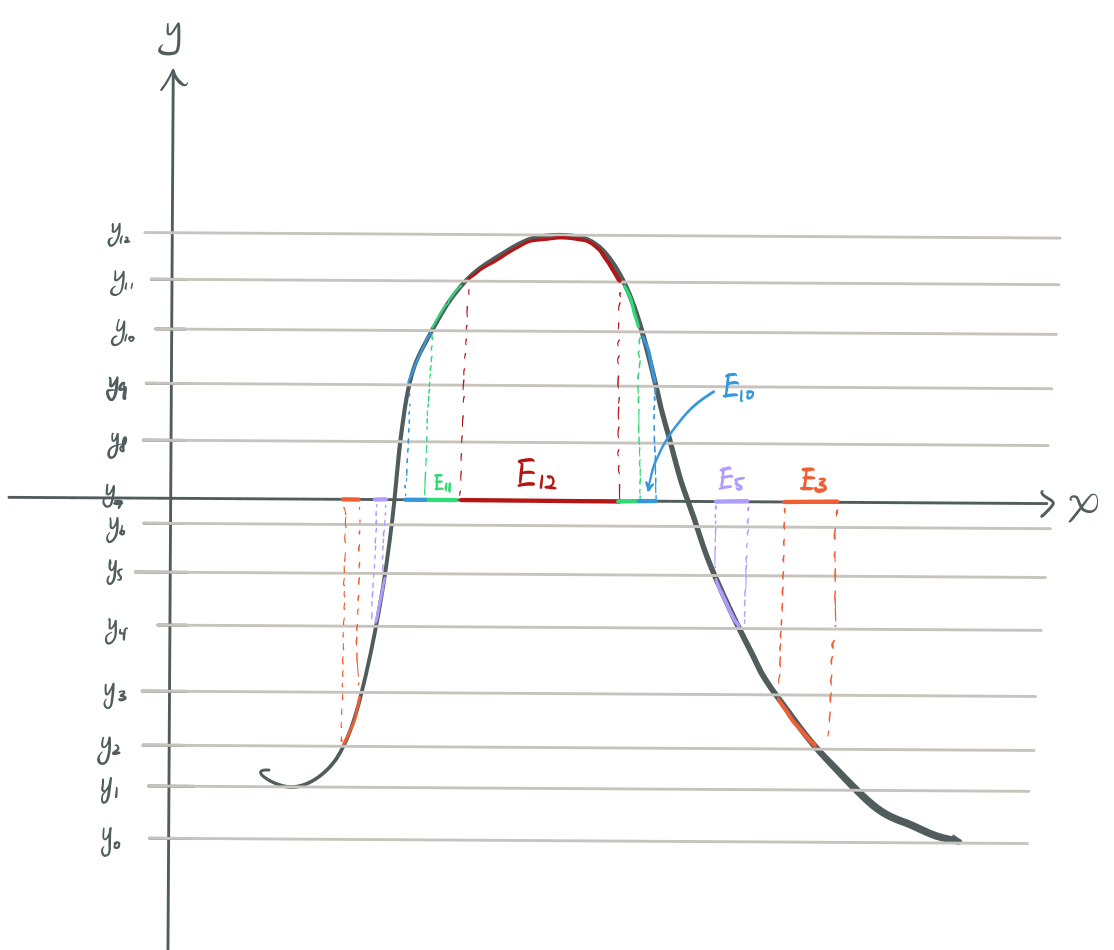
\includegraphics[width=0.5\linewidth]{images/heuristic_into_lesbesgue_integration.png}
  \caption{A sketch of what's happening with the construction of the $E_k$'s}
  \label{fig:a_sketch_of_what_s_happening_with_the_construction_of_the_e_k_s}
\end{figure*}

This will then allow us to estimate the integral of $f$ over $[a, b]$ by the
expression
\begin{equation*}
  \sum_{k=1}^{N} y_k m E_k,
\end{equation*}
where each of the $y_k m E_k$ are called \hlnotea{simple functions}. In the
expression, $mE_k$ denotes a ``measure'' \sidenote{Note that a measure is simply
a generalization of the notion of `length'.} of $E_k$.

\begin{figure*}[ht]
  \centering
  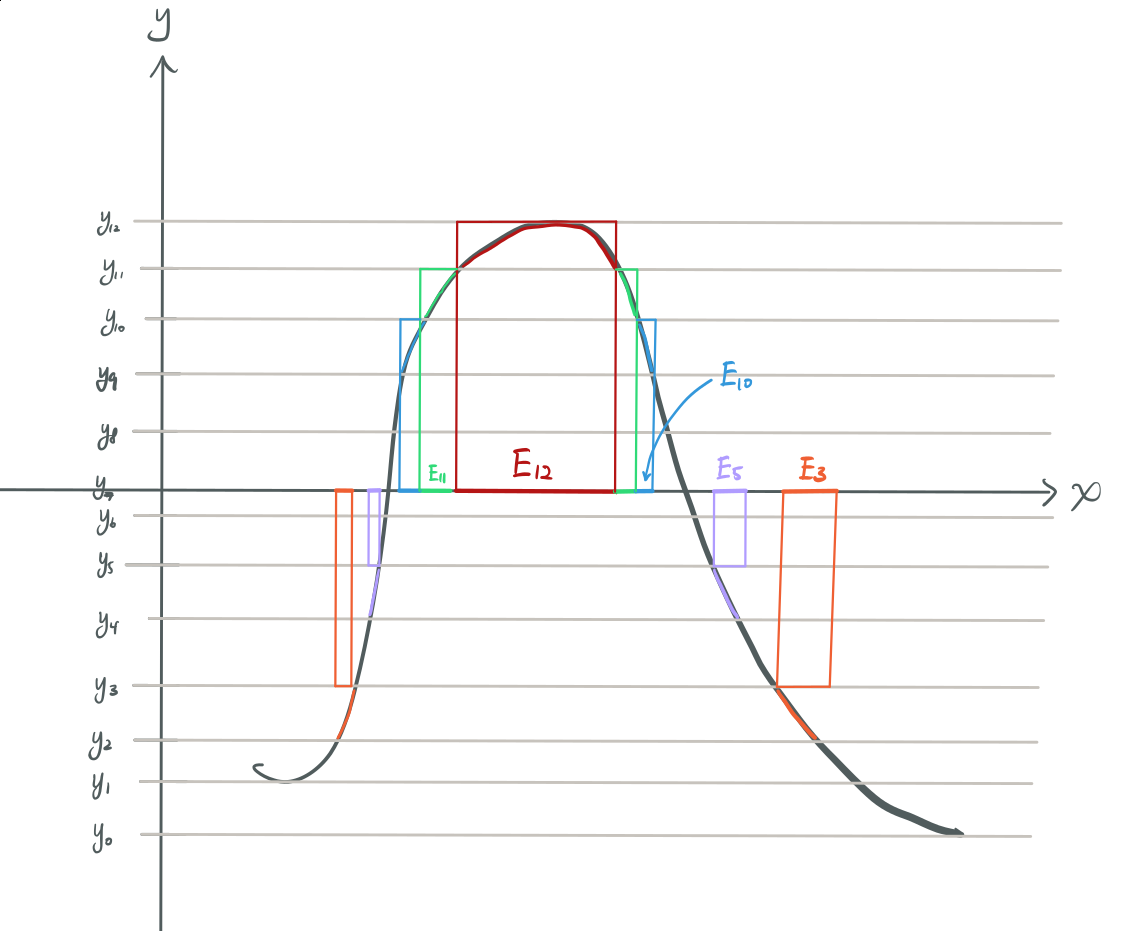
\includegraphics[width=0.5\linewidth]{images/heuristic_into_lesbesgue_integration_heaps.png}
  \caption{Drawing out the rectangles of $y_k mE_k$ from
  \cref{fig:a_sketch_of_what_s_happening_with_the_construction_of_the_e_k_s}.}
  \label{fig:drawing_out_the_rectangles_of_y_k_me_k_from_fig_}
\end{figure*}

We observe that $E_k$ need not be a particularly well-behaved set. However, note
that we may rearrange the possibly scattered pieces of each $E_k$ together, so
as to form a `continuous' base for the rectangle. We need our definition of a
measure to be able to capture this.

The following is an analogy from Lebesgue himself on comparing Lebesgue
integration and Riemann integration \cite{siegmund2008}:

\begin{quotebox}{magenta}{foreground}
  I have to pay a certain sum, which I have collected in my pocket. I take the
  bills and coins out of my pocket and give them to the creditor in the order I
  find them until I have reached the total sum. This is the Riemann integral.

  But I can proceed differently. After I have taken all the money out of my
  pocket I order the bills and coins according to identical values and then I
  pay the several heaps one after the other to the creditor. This is my
  integral.
\end{quotebox}

The insight here is that one can \hlbnotea{freely arrange} the values of the
functions, all the while \hlbnotea{preserving} the value of the integral.
\begin{itemize}
  \item This requires us to have a better understanding of what a measure is.
  \item This process of rearrangement converts certain functions which are
    extremely difficult to deal with, or outright impossible, with the Riemann
    integral, into easily digestible pieces using Lebesgue integral.
\end{itemize}

% section riemannian_integration_continued (end)

\section{Lebesgue Outer Measure}%
\label{sec:lebesgue_outer_measure}
% section lebesgue_outer_measure

\paragraph{Goals of the section}

\begin{enumerate}
  \item Define a ``measure of length'' on as many subsets of $\mathbb{R}$ as
    possible.
  \item The definition should agree with our intuition of what a `length' is.
\end{enumerate}

\begin{defn}[Length]\index{Length}\label{defn:length}
  For $a \leq b \in \mathbb{R}$, we define the \hlnoteb{length} of the interval
  $(a, b)$ to be $b - a$, and we write
  \begin{equation*}
    \ell((a, b)) \coloneqq b - a.
  \end{equation*}
  We also define
  \begin{itemize}
    \item $\ell(\emptyset) = 0$; and
    \item $\ell((a, \infty)) = \ell((-\infty, b)) = \ell((-\infty, \infty)) =
      \infty$.
  \end{itemize}
\end{defn}

\begin{defn}[Cover by Open Intervals]\index{Cover by Open Intervals}\label{defn:cover_by_open_intervals}
  Let $E \subseteq \mathbb{R}$. A countable collection $\{ I_n
  \}_{n=1}^{\infty}$ of open intervals is said to be a \hlnoteb{cover of $E$ by
  open intervals} if $E \subseteq \bigcup_{n=1}^{\infty} I_n$.
\end{defn}

\begin{note}
  In this course, the only covers that we shall use are \hlbnotec{open
  intervals}, and so we shall henceforth refer to the above simply as covers of
  $E$.
\end{note}

Before giving what immediately follows from the above, I shall present the
following notion of an outer measure.

\begin{defn}[Outer Measure]\index{Outer Measure}\label{defn:outer_measure}
  Let $\emptyset \neq X$ be a set. An \hlnoteb{outer measure} $\mu$ on $X$ is a
  function
  \begin{equation*}
    \mu : \mathcal{P}(X) \to [0, \infty] \coloneqq [0, \infty) \cup \{ \infty \}
  \end{equation*}
  which satisfies
  \begin{marginfigure}
    \centering
    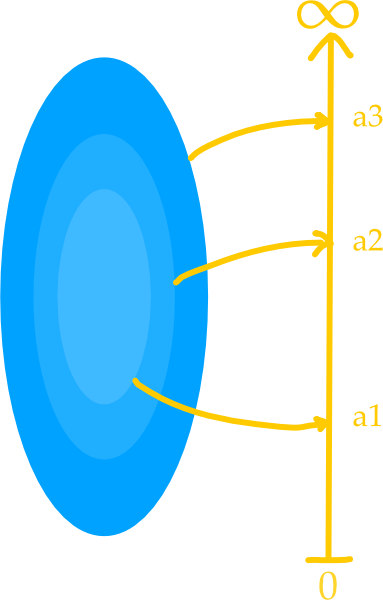
\includegraphics[width=0.8\marginparwidth]{images/outermeasure.png}
    \caption{Idea of the outer measure}\label{fig:idea_of_the_outer_measure}
  \end{marginfigure}
  \begin{enumerate}
    \item $\mu \emptyset = 0$;
    \item (\hldefn{monotone increment} or \hldefn{monotonicity}) $E \subseteq F
      \subseteq X \implies \mu E \leq \mu F$; and
    \item (\hldefn{countable subadditivity} or
      \hldefn{$\sigma$-subadditivity}) $\{ E_n \}_{n=1}^{\infty} \subseteq
      \mathcal{P}(X)$
       \begin{equation*}
        \mu \left( \bigcup_{n=1}^{\infty} E_n \right) \leq \sum_{n=1}^{\infty}
        \mu E_n.
      \end{equation*}
  \end{enumerate}
\end{defn}

\begin{note}
  Note that by the monotonicity, the $\sigma$-subadditivity condition is
  equivalent to: given $\{ E_n \}_{n=1}^{\infty} \subseteq \mathcal{P}(X)$ and
  $F \subseteq \bigcup_{n=1}^{\infty} E_n$, we have that
  \begin{equation*}
    \mu(F) \leq \sum_{n=1}^{\infty} \mu(E_n).
  \end{equation*}
\end{note}

\begin{defn}[Lebesgue Outer Measure]\index{Lebesgue Outer Measure}\label{defn:lebesgue_outer_measure}
  We define the \hlnoteb{Lebesgue outer measure} as a function $m^* :
  \mathcal{P}(X) \to \mathbb{R}$ such that
  \begin{equation*}
    m^* E \coloneqq \inf \left\{ \sum_{n=1}^{\infty} \ell(I_n) : E \subseteq
    \bigcup_{n=1}^{\infty} I_n \right\}.
  \end{equation*}
\end{defn}

We cheated a little bit by calling the above an outer measure, so let us now
justify our cheating.

\begin{propo}[Validity of the Lebesgue Outer Measure]\label{propo:validity_of_the_lebesgue_outer_measure}
  $m^*$ is indeed an outer measure.
\end{propo}

\begin{proof}
  \hlbnoted{$\mu \emptyset = 0$} We consider a sequence of sets $\{ I_n
  \}_{n=1}^{\infty}$ such that $I_n = \emptyset$ for each $n = 1, \ldots,
  \infty$. It is clear that $\emptyset \subseteq \bigcup_{n=1}^{\infty} I_n$.
  Also, we have that $\ell(I_n) = 0$ for all $n = 1, \ldots, \infty$. It follows
  that
  \begin{equation*}
    0 \leq m^*(\emptyset) \leq \sum_{n=1}^{\infty} m^* (I_n) =
    \sum_{n=1}^{\infty} 0 = 0,
  \end{equation*}
  where the inequality is simply by the definition of $m^*$ being an infimum,
  \hlimpo{not to be confused with $\sigma$-subadditivity}. We thus have that
  \begin{equation*}
    m^*(\emptyset) = 0.
  \end{equation*}

  \noindent
  \hlbnoted{Monotonicity} Suppose $E \subseteq F \subseteq
  \mathbb{R}$, and $\{ I_n \}_{n=1}^{\infty}$ a cover of $F$. Then
  \begin{equation*}
    E \subseteq F \subseteq \bigcup_{n=1}^{\infty} I_n.
  \end{equation*}
  In particular, all covers of $F$ are also covers of $E$, i.e.
  \begin{equation*}
    \left\{ \{ J_m \}_{m=1}^{\infty} : E \subseteq \bigcup_{m=1}^{\infty} J_m \right\}
    \subseteq
    \left\{ \{ I_n \}_{n=1}^{\infty} : F \subseteq \bigcup_{n=1}^{\infty} I_n \right\}.
  \end{equation*}
  It follows that
  \begin{equation*}
    m^* E \leq m^* F.
  \end{equation*}

  \noindent
  \hlbnoted{$\sigma$-subaddivitity} Consider $\{ E_n \}_{n=1}^{\infty} \subseteq
  \mathcal{P}(X)$ such that $E \subseteq \bigcup_{n=1}^{\infty} E_n$. WTS
  \begin{equation*}
    m^* E \leq \sum_{n=1}^{\infty} m^* E_n.
  \end{equation*}

  Now if the sum of the RHS is infinite, i.e. if any of the $m^* E_n$ is
  infinite, then the inequality comes for free. Thus WMA $\sum_{n=1}^{\infty}
  E_n < \infty$, and in particular that $m^* E_n < \infty$ for all $n = 1,
  \ldots, \infty$.

  To do this, let $\epsilon > 0$. Since $m^* E_n < \infty$ for all $n$, we can
  find covers $\left\{ I_k^{(n)} \right\}_{k=1}^{\infty}$ for each of the
  $E_n$'s such that
  \begin{equation*}
    \sum_{k=1}^{\infty} \ell\left(I_k^{(n)}\right) < m^* E_n +
    \frac{\epsilon}{2^n}.
  \end{equation*}
  Then, we have that
  \begin{equation*}
    E \subseteq \bigcup_{n=1}^{\infty} E_n \subseteq \bigcup_{n=1}^{\infty}
    \bigcup_{k=1}^{\infty}  I_k^{(n)}.
  \end{equation*}
  Then by $m^* E$ being the infimum of the sum of lengths of the covering
  intervals, we have that
  \begin{align*}
    m^* E &\leq \sum_{n=1}^{\infty} \sum_{k=1}^{\infty} \ell \left( I_k^{(n)}
            \right) \\
          &\leq \sum_{n=1}^{\infty} \left( m^* E_n + \frac{\epsilon}{2^n}
            \right) \\
          &= \sum_{n=1}^{\infty} m^* E_n + \sum_{n=1}^{\infty}
            \frac{\epsilon}{2^n} \\
          &= \sum_{n=1}^{\infty} m^* E_n + \epsilon.
  \end{align*}
  Since $\epsilon$ was arbitrary, we have that
  \begin{equation*}
    m^* E_n \leq \sum_{n=1}^{\infty} m^* E_n,
  \end{equation*}
  as desired.
\end{proof}

\begin{crly}[Lebesgue Outer Measure of Countable Sets is Zero]\label{crly:lebesgue_outer_measure_of_countable_sets_is_zero}
  If $E \subseteq \mathbb{R}$ is countable, then $m^* E = 0$.
\end{crly}

\begin{proof}
  We shall prove for when $E$ is denumerable, for the finite case follows a
  similar proof. Let us write $E = \{ x_n \}_{n=1}^{\infty}$. Let $\epsilon > 0$ 
  and
  \begin{equation*}
    I_n = \left( x_n - \frac{\epsilon}{2^{n+1}},\, x_n + \frac{\epsilon}{2^{n+1}}
    \right).
  \end{equation*}
  Then it is clear that $\{ I_n \}_{n=1}^{\infty}$ is a cover of $E$.
  
  It follows that
  \begin{equation*}
    0 \leq m^* E \leq \sum_{n=1}^{\infty} \ell (I_n) = \sum_{n=1}^{\infty}
    \frac{\epsilon}{2^n} = \epsilon.
  \end{equation*}
  Thus as $\epsilon \to 0$, we have that
  \begin{equation*}
    m^* E = 0,
  \end{equation*}
  as expected.
\end{proof}

\begin{crly}[Lebesgue Outer Measure of $\mathbb{Q}$ is Zero]\label{crly:lebesgue_outer_measure_of_q_is_zero}
  We have that $m^* \mathbb{Q} = 0$.
\end{crly}

\newthought{In the proofs} above that we have looked into, and based on the
intuitive notion of the length of an open interval, it is compelling to simply
conclude that
\begin{equation*}
  m^* (a, b) = \ell(a, b) = b - a.
\end{equation*}
However, looking back at \cref{defn:lebesgue_outer_measure}, we know that that
is not how $m^* (a, b)$ is defined.

This leaves us with an interesting question:
\begin{quotebox}{green}{foreground}
  how does our notion of measure $m^*(a, b)$ of an interval compare with the
  notion of the length of an interval?
\end{quotebox}

By taking $I_1 = (a, b)$ and $I_n = \emptyset$ for $n \geq 2$, it is rather
clear that $\{ I_n \}_{n=1}^{\infty}$ is a cover of $(a, b)$, and so we have
\begin{equation}\label{eq:lebesgue_outer_measure_leq_length}
  m^* (a, b) \leq \ell(a, b) = b - a.
\end{equation}
However, the other side of the game is not as easy to confirm: we would have to
consider \hlimpo{all} possible covers of $(a, b)$, which is a lot.

Another question that we can ask ourselves seeing
\cref{eq:lebesgue_outer_measure_leq_length} is why can't $m^*(a, b)$ be
something that is strictly less than the length to give us an even more
`precise' measurement?

To answer these questions, it is useful to first consider the outer measure of a
closed and bounded interval, e.g. $[a, b]$, since these intervals are
\hlnotea{compact} under the \hlnotea{Heine-Borel Theorem}. This will give us a
finite subcover for every infinite cover of the compact interval, which is easy
to deal with.

We shall see that with the realization of the outer measure of a compact
interval, we will also be able to find the outer measure of intervals that are
neither open nor closed.

We shall prove the following proposition in the next lecture. Note that for the
sake of presentation, I shall abbreviate the Lebesgue Outer Measure as LOM.

\begin{propononum}[LOM of Arbitrary Intervals]
  Suppose $a < b \in \mathbb{R}$. Then
  \begin{enumerate}
    \item $m^*([a, b]) = b - a$; and therefore
    \item $m^*((a, b]) = m^*([a, b)) = m^*((a, b)) = b - a$.
  \end{enumerate}
\end{propononum}

% section lebesgue_outer_measure (end)

% chapter lecture_2_may_9th_2019 (end)

\chapter{Lecture 3 May 14th 2019}%
\label{chp:lecture_3_may_14th_2019}
% chapter lecture_3_may_14th_2019

\section{Lebesgue Outer Measure Continued}%
\label{sec:lebesgue_outer_measure_continued}
% section lebesgue_outer_measure_continued

\begin{propo}[LOM of Arbitrary Intervals]\label{propo:lom_of_arbitrary_intervals}
  Suppose $a < b \in \mathbb{R}$. Then
  \begin{enumerate}
    \item $m^*([a, b]) = b - a$; and therefore
    \item $m^*((a, b]) = m^*([a, b)) = m^*((a, b)) = b - a$.
  \end{enumerate}
\end{propo}

\begin{proof}
  \begin{enumerate}
    \item Consider $a < b \in \mathbb{R}$. Let $\epsilon > 0$, and let
      \begin{equation*}
        I_1 = \left( a - \frac{\epsilon}{2}, \, b + \frac{\epsilon}{2} \right)
      \end{equation*}
      and $I_n = \emptyset$ for $n \geq 2$. Then $\{ I_n \}_{n=1}^{\infty}$ is a
      cover of $[a, b]$. This means that
      \begin{equation*}
        m^*([a, b]) \leq \sum_{n=1}^{\infty} \ell(I_n) = b - a + \epsilon.
      \end{equation*}
      So for all $\epsilon \to 0$, we have that
      \begin{equation*}
        m^*([a, b]) \leq b - a.
      \end{equation*}

      \sidenote{For the converse, we know that $m^*([a, b]) = \inf \faStar$,
      where $\faStar$ is just a placeholder for you-know-what. So $m^*([a,
      b])$ is one of the sums. So if we can show that for an arbitrary sum,
      $\geq$ holds, our work is done.} Conversely, if $[a, b]$ is covered by open
      intervals $\{ I_n \}_{n=1}^{\infty}$, then by compactness of $[a, b]$ (via
      the \hlnotea{Heine-Borel Theorem}), we know that we can cover $[a, b]$ by
      finitely many of these intervals, and let us denote these as $\{ I_n
      \}_{n=1}^{N}$, for some $1 \leq N < \infty$.

      WTS
      \begin{equation*}
        \sum_{n=1}^{N} \ell(I_n) \geq b - a.
      \end{equation*}
      If LHS $= \infty$, then our work is done. Thus wlog, WMA each $I_n = (a_n,
      b_n)$ is a finite interval. Note that we have
      \begin{equation*}
        [a, b] \subseteq \bigcup_{n=1}^{N} (a_n, b_n).
      \end{equation*}
      In particular, $a \in \bigcup_{n=1}^{N} I_n$. Thus, $\exists 1 \leq n_2
      \leq N$ such that $a \in I_{n_1}$. Now if $b_{n_1} > b$, we shall stop
      this process for our work is done, since then $[a, b] \subseteq I_{n_1}$.
      Otherwise, if $b_{n_1} \leq b$, then $b_{n_1} \in [a, b] \subseteq
      \bigcup_{n=1}^{N} I_n$, which means that $\exists 1 \leq n_2 \leq N$ such
      that $b_{n_1} \in I_{n_2}$.
      \begin{figure*}[ht]
        \centering
        \begin{tikzpicture}
          \draw (-7, 0) -- (7, 0);
          \draw (-4, 0.2) -- (-4, -0.2) node[below] {$a$};
          \draw (4, 0.2) -- (4, -0.2) node[below] {$b$};
          \draw[
            {Arc Barb[length=5pt,width=15pt]}-{Arc Barb[length=5pt,width=15pt]},red
            ] (-5,0) node[above=10pt] {$a_{n_1}$} -- (-2,0) node[above=10pt]
            {$b_{n_1}$};
          \draw[
            {Arc Barb[length=5pt,width=15pt]}-{Arc Barb[length=5pt,width=15pt]},cyan
            ] (-3,0) node[above=10pt] {$a_{n_2}$} -- (0,0) node[above=10pt]
            {$b_{n_2}$};
          \node at (1, 0.6) {$\hdots$};
          \draw[
            {Arc Barb[length=5pt,width=15pt]}-{Arc Barb[length=5pt,width=15pt]},magenta
            ] (2,0) node[above=10pt] {$a_{n_k}$} -- (5,0) node[above=10pt]
            {$b_{n_k}$};
        \end{tikzpicture}
        \caption{Our continual picking of $I_{n_1}, I_{n_2}, \ldots, I_{n_k}$}
        \label{fig:our_continual_picking_of_i__n_1_i__n_2_ldots_i__n_k_}
      \end{figure*}
      Notice that $n_1 \neq n_2$, since $b_{n_1} \notin I_{n_1}$ but $b_{n_1}
      \in I_{n_2}$.

      Now once again, if $b_{n_2} > b$, then we shall stop this process since
      our work is done. Otherwise, we have $a < b_{n_2} \leq b$, and so $\exists
      1 \leq n_3 \leq N$, $n_3 \neq n_1, n_2$, such that $b_{n_2} \in I_3$...

      We continue with the above process for as long as $b_{n_k} \leq b$. We can
      thus find, for each $k$, $I_{n_{k+1}}$, where $n_{k+1} \in \{ 1, \ldots, N
      \} \setminus \{ n_1, n_2, \ldots, n_k \}$, such that $b_{n_k} \in
      I_{n_{k+1}}$.

      However, since each of the $I_{n_k}$'s are different, and since we only
      have $N$ such intervals, there must exists a $K \leq N$ such that
      \begin{equation*}
        b_{n_{K-1}} \leq b \text{ and } b_{n_K} > b.
      \end{equation*}

      It now suffices for us to show that
      \begin{equation*}
        \sum_{j=1}^{K} \ell(I_{n_j}) \geq b - a.
      \end{equation*}

      Observe that
      \begin{align*}
        \sum_{j=1}^{K} \ell(I_{n_j})
        &= (b_{n_K} - a_{n_K}) + (b_{n_{K-1}} - a_{n_{K-1}}) + \hdots \\
        &\quad + (b_{n_2} - a_{n_2}) + (b_{n_1} - a_{n_1}) \\
        &= b_{n_K} + \underset{\geq 0}{(b_{n_{K-1}} - a_{n_K})} + \underset{\geq
          0}{(b_{n_{K-2}} - a_{n_{K-1}})} + \hdots \\
        &\quad + \underset{\geq 0}{(b_{n_1} - a_{n_2})} - a_{n_1} \\
        &\geq b_{n_K} - a_{n_1} \geq b - a.
      \end{align*}
      Thus
      \begin{equation*}
        \sum_{n=1}^{\infty} \ell(I_n) \geq \sum_{n=1}^{N} \ell(I_n) \geq
        \sum_{j=1}^{K} \ell(I_{n_j}) \geq b - a,
      \end{equation*}
      whence
      \begin{equation*}
        m^*([a, b]) \geq b - a.
      \end{equation*}

      It follows that, indeed,
      \begin{equation*}
        m^*([a, b]) = b - a.
      \end{equation*}

    \item First, note that
      \begin{equation*}
        m^*((a, b)) \leq m^*([a, b]) \leq b - a.
      \end{equation*}
      On the other hand, notice that $\forall 0 < \epsilon < \frac{b - a}{2}$,
      we have that
      \begin{equation*}
        [a + \epsilon, b - \epsilon] \subseteq (a, b),
      \end{equation*}
      and so by monotonicity,
      \begin{equation*}
        (b - a) - 2 \epsilon = m^*([a + \epsilon, b - \epsilon]) \leq m^*((a,
        b)).
      \end{equation*}
      As $\epsilon \to 0$, we have that
      \begin{equation*}
        b - a \leq m^*((a, b)) \leq b - a.
      \end{equation*}
      So
      \begin{equation*}
        m^*((a, b)) = b - a
      \end{equation*}
      as desired.

      Finally, we have that
      \begin{equation*}
        b - a = m^*((a, b)) \leq m^*((a, b]) \leq m^*([a, b]) = b - a,
      \end{equation*}
      and similarly
      \begin{equation*}
        b - a = m^*((a, b)) \leq m^*([a, b)) \leq m^*([a, b]) = b - a.
      \end{equation*}
      Thus
      \begin{equation*}
        m^*((a, b)) = m^*((a, b]) = m^*([a, b)) = b - a
      \end{equation*}
      as required.
  \end{enumerate}
\end{proof}

\begin{propo}[LOM of Infinite Intervals]\label{propo:lom_of_infinite_intervals}
  We have that $\forall a, b \in \mathbb{R}$,
  \begin{align*}
    m^*((a, \infty)) &= m^*([a, \infty)) \\
                     &= m^*((-\infty, b)) = m^*((-\infty, b]) \\
                     &= m^* \mathbb{R} = \infty.
  \end{align*}
\end{propo}

\begin{proof}
  Observe that
  \begin{equation*}
    (a, a + n) \subseteq (a, \infty)
  \end{equation*}
  for all $n \geq 1$. Thus
  \begin{equation*}
    n = m^*((a, a + n)) \leq m^*((a, \infty))
  \end{equation*}
  for all $n \geq 1$. Hence
  \begin{equation*}
    m^*((a, \infty)) = \infty
  \end{equation*}
  by definition.

  All other cases follow similarly.
\end{proof}

\begin{crly}[Uncountability of $\mathbb{R}$]\label{crly:uncountability_of_r}
  $\mathbb{R}$ is uncountable.
\end{crly}

\begin{proof}
  We have that
  \begin{equation*}
    m^* \mathbb{R} = \infty \neq 0,
  \end{equation*}
  and so it follows from
  \cref{crly:lebesgue_outer_measure_of_countable_sets_is_zero}, we must have
  that $\mathbb{R}$ is uncountable.
\end{proof}

\begin{defn}[Translation Invariant]\index{Translation Invariant}\label{defn:translation_invariant}
  Let $\mu$ be an \hyperref[defn:outer_measure]{outer measure} on $\mathbb{R}$.
  We say that $\mu$ is \hlnoteb{translation invariant} if $\forall E \subseteq
  \mathbb{R}$,
  \begin{equation*}
    \mu(E) = \mu(E + \kappa)
  \end{equation*}
  for all $\kappa \in \mathbb{R}$, where
  \begin{equation*}
    E + \kappa \coloneqq \{ x + \kappa : x \in E \}.
  \end{equation*}
\end{defn}

\begin{propo}[Translation Invariance of the LOM]\label{propo:translation_invariance_of_the_lom}
  The Lebesgue outer measure is translation invariant.
\end{propo}

\begin{proof}
  Let $E \subseteq \mathbb{R}$ and $\kappa \in \mathbb{R}$. Note that $E$ is
  covered by open intervals $\{ I_n \}_{n=1}^{\infty}$ iff $E + \kappa$ is
  covered by $\{ I_n + \kappa \}_{n=1}^{\infty}$.

  \noindent
  \hlbnoted{Claim: $\forall n \geq 1$, $\ell(I_n + \kappa) = \ell(I_n)$} Write
  \begin{equation*}
    I_n = (a_n, b_n).
  \end{equation*}
  Then
  \begin{equation*}
    I_n + \kappa = (a_n + \kappa, b_n + \kappa).
  \end{equation*}
  Observe that
  \begin{equation*}
    \ell(I_n + \kappa) = b_n + \kappa - (a_n - \kappa) = b_n - a_n = \ell(I_n),
  \end{equation*}
  as claimed. $\dashv$

  By the claim, it follows that
  \begin{align*}
    m^*(E) &= \inf \left\{ \sum_{n=1}^{\infty} \ell(I_n) : E \subseteq
            \bigcup_{n=1}^{\infty} \right\} \\
           &= \inf \left\{ \sum_{n=1}^{\infty} \ell(I_n + \kappa) : E + \kappa \subseteq
           \bigcup_{n=1}^{\infty} (I_n + \kappa)  \right\} \\
           &= m^*(E + \kappa).
  \end{align*}
\end{proof}

\begin{remark}
  Suppose $E \subseteq \mathbb{R}$ and $E = \bigcup_{n=1}^{\infty} E_n$,
  where
  \begin{equation*}
    E_i \cap E_j = \emptyset \text{ if } i \neq j.
  \end{equation*}
  Now by $\sigma$-subadditivity of $m^*$, we have that
  \begin{equation*}
    m^* E \leq \sum_{n=1}^{\infty} m^* E_n.
  \end{equation*}

  However, equality is not guaranteed. Consider the following case: if $E = [0,
  1]$, we may have $E_n = [0, 1]$ for all $n >= 1$, in which case $E =
  \bigcup_{n=1}^{\infty} E_n = [0, 1]$, but
  \begin{equation*}
    m^* E = m^* [0, 1] = 1 < \infty = \sum_{n=1}^{\infty} m^* E_n.
  \end{equation*}

  It would be desirable to have
  \begin{equation*}
    m^* E = \sum_{n=1}^{\infty} m^* E_n,
  \end{equation*}
  when the $E_i$'s are pairwise disjoint, i.e. $E = \bigcupdot_{n=1}^{\infty}
  E_n$. In fact, this would agree with our intuition, that if the outer measure
  is going to be our `length'. Consider the example $A = [0, 2] \cup [5, 7]$.
  Then we would expect $m^* A = 2 + 2 = 4$.

  However, this is actually impossible for an arbitrary number of collections.
\end{remark}

\begin{thm}[Non-existence of a sensible Translation Invariant Outer Measure that is also $\sigma$-additive]\label{thm:non_existence_of_a_sensible_translation_invariant_outer_measure_that_is_also_sigma_additive}
  There does not exist a translation-invariant outer measure $\mu$ on
  $\mathbb{R}$ that satisfies
  \begin{enumerate}
    \item $\mu(\mathbb{R}) > 0$;
    \item $\mu[0, 1] < \infty$; and
    \item $\mu$ is \hldefn{$\sigma$-additive}; i.e. if $\{ E_n
      \}_{n=1}^{\infty}$ is a countable collection of disjoint subsets of
      $\mathbb{R}$ that covers $E \subseteq \mathbb{R}$, then
      \begin{equation*}
        \mu E = \sum_{n=1}^{\infty} \mu E_n.
      \end{equation*}
  \end{enumerate}
  Consequently, the \hyperref[defn:lebesgue_outer_measure]{Lebesgue outer
  measure} $m^*$ is \hlimpo{not} $\sigma$-additive.
\end{thm}

\begin{proof}
  Suppose to the contrary that such a $\mu$ exists.

  \noindent
  \hlbnoteb{Step 1} Consider the relation $\sim$ on $\mathbb{R}$ such that $x
  \sim y$ if $x - y \in \mathbb{Q}$.

  \noindent
  \hlbnoted{Claim: $\sim$ is an equivalence relation}
  \begin{itemize}
    \item (\textbf{reflexivity}) We know that $0 \in \mathbb{Q}$ and $x - x = 0$.
      Thus $x \sim x$.
    \item (\textbf{symmetry}) Since $\mathbb{Q}$ is a \hlnotea{field}, it is
      closed under multiplication, and $-1 \in \mathbb{Q}$. Thus if $x \sim y$,
      then $x - y \in \mathbb{Q}$, and so $(-1)(x - y) = y - x \in \mathbb{Q}$,
      which means $y \sim x$.
    \item (\textbf{transitivity}) Again, since $\mathbb{Q}$ is a field, it is
      closed under (this time) addition. Thus
      \begin{align*}
        &x \sim y \, \land \, y \sim z \implies (x - y), \, (y - z) \in
        \mathbb{Q} \\
        &\implies (x - y) + (y - z) = x - z \in \mathbb{Q}.
      \end{align*}
      Thus $x \sim z$.
  \end{itemize}
  This proves the claim. $\dashv$

  Let
  \begin{equation*}
    [x] \coloneqq x + \mathbb{Q} \coloneqq \{ x + q : q \in \mathbb{Q} \}
  \end{equation*}
  denote the equivalence class of $x$ wrt $\sim$. Note that the set of
  equivalence classes, which we shall represent as
  \begin{equation*}
    \mathcal{F} \coloneqq \{ [x] : x \in \mathbb{R} \},
  \end{equation*}
  partitions $\mathbb{R}$, i.e.
  \begin{itemize}
    \item $[x] = [y] \iff x - y \in \mathbb{Q}$; and
    \item $[x] \cap [y] = \emptyset$ otherwise.
  \end{itemize}

  Note that since $\mathbb{Q}$ is \hlnotea{dense} in $\mathbb{R}$, we have that
  $[x] = x + \mathbb{Q}$ is also dense in $\mathbb{R}$, for all $x \in
  \mathbb{R}$. Then for each \sidenote{Notice that here, we
  have invoked the \hlbnotee{Axiom of Choice}.} $F \in \mathcal{F}$, $\exists
  x_F \in F$ such that
  \begin{equation*}
    0 \leq x_F \leq 1.
  \end{equation*}
  Now consider the set
  \begin{equation*}
    \mathbb{V} \coloneqq \{ x_F : F \in \mathcal{F} \} \subseteq [0, 1],
  \end{equation*}
  which is called \hldefn{Vitali's Set}.

  \noindent
  \hlbnoteb{Step 2} Since $\mathcal{F}$ partitions $\mathbb{R}$, we have that
  \begin{align*}
    \mathbb{R} &= \bigcupdot_{F \in \mathcal{F}} F = \bigcupdot_{F \in
                 \mathcal{F}} [x_F] \\
               &= \bigcupdot_{F \in \mathcal{F}} x_F + \mathbb{Q} \\
               &= \mathbb{V} + \mathbb{Q} \coloneqq \{ x + q : q \in \mathbb{Q},
                x \in \mathbb{V} \}.
  \end{align*}

  \noindent
  \hlbnoteb{Step 3} \hlbnoted{Claim: $p \neq q \in \mathbb{Q} \implies
  (\mathbb{V} + p) \cap (\mathbb{V} + q) = \emptyset$} Suppose not, and suppose
  $\exists y \in (\mathbb{V} + p) \cap (\mathbb{V} + q)$. Then $\exists F_1, F_2
  \in \mathcal{F}$ such that
  \begin{equation}\label{eq:nonexistence_of_transinvar_outmea_eq1}
    y = x_{F_1} + p = x_{F_2} + q.
  \end{equation}
  Then we may rearrange the above equation to get
  \begin{equation*}
    x_{F_1} - x_{F_2} = q - p \in \mathbb{Q}.
  \end{equation*}
  This implies that
  \begin{equation*}
    [x_{F_1}] = [x_{F_2}] \implies F_1 = F_2
  \end{equation*}
  since $\mathbb{V}$ consists of one unique representative from each of the
  equivalence classes. However, this would mean that
  \begin{equation*}
    x_{F_1} = x_{F_2}.
  \end{equation*}
  Since $p \neq q$, we have that
  \begin{equation*}
    x_{F_1} + p \neq x_{F_2} + q,
  \end{equation*}
  which contradicts \cref{eq:nonexistence_of_transinvar_outmea_eq1}. Thus
  \begin{equation*}
    (\mathbb{V} + p) \cap (\mathbb{V} + q) = \emptyset,
  \end{equation*}
  as claimed. $\dashv$

  This in turn means that the $\mathbb{V} + q$, for each $q \in \mathbb{Q}$,
  also partitions $\mathbb{R}$. In other words, if we write $\mathbb{Q} = \{ p_n
  \}_{n=1}^{\infty}$, then
  \begin{equation*}
    \mathbb{R} = \mathbb{V} + \mathbb{Q} = \bigcupdot_{n=1}^{\infty} \mathbb{V}
    + p_n.
  \end{equation*}

  Now, note that
  \begin{equation*}
    0 \neq \mu \mathbb{R} \overset{(1)}{=} \sum_{n=1}^{\infty} \mu(\mathbb{V} +
    p_n) \overset{(2)}{=} \sum_{n=1}^{\infty} \mu(\mathbb{V}),
  \end{equation*}
  where $(1)$ is by $\mu$ being $\sigma$-additive and $(2)$ is by $\mu$ being
  translation invariant, both directly from our assumptions. This means that
  \begin{equation*}
    \mu \mathbb{V} > 0.
  \end{equation*}

  \noindent
  \hlbnoteb{Step 4} Now consider $S = \mathbb{Q} \cap [0, 1]$ such that $S$ is
  denumerable. Write
  \begin{equation*}
    S = \{ s_n \}_{n=1}^{\infty}.
  \end{equation*}
  Note that for all $n \geq 1$,
  \begin{equation*}
    \mathbb{V} \subseteq [0, 1] \implies \mathbb{V} + s_n \subseteq [0, 2],
  \end{equation*}
  and as proven above
  \begin{equation*}
    i \neq j \implies (\mathbb{V} + s_i) \cap (\mathbb{V} + s_j) = \emptyset.
  \end{equation*}

  Thus it follows that
  \begin{equation*}
    \mu \left( \bigcupdot_{n=1}^{\infty} \mathbb{V} + s_n \right)
    = \sum_{n=1}^{\infty} \mu (\mathbb{V} + s_n) 
    = \sum_{n=1}^{\infty} \mu(\mathbb{V})
    = \infty.
  \end{equation*}
  Also,
  \begin{align*}
    \mu \left( \bigcupdot_{n=1}^{\infty} \mathbb{V} + s_n \right)
    &= \sum_{n=1}^{\infty} \mu (\mathbb{V} + s_n) \\
    &\leq \mu([0, 2]) = \mu([0, 1] \cup ([0, 1] + 1)) \\
    &\leq \mu[0, 1] + \mu([0, 1] + 1) \\
    &= 2 \mu([0, 1]) = 2 < \infty,
  \end{align*}
  contradicting what we have right above.

  Therefore, no such $\mu$ exists.
\end{proof}

With the realization of
\cref{thm:non_existence_of_a_sensible_translation_invariant_outer_measure_that_is_also_sigma_additive},
we find ourselves facing a losing dilemma: we may either
\begin{enumerate}
  \item be happy with the Lebesgue outer measure $m^*$ for \hlbnotee{all}
    subsets $E \subseteq \mathbb{R}$, which would \hlbnotec{agree with our
    intuitive notion} of length, at the price of $\sigma$-additivity; or
  \item restrict the \hlbnotee{domain} of our function $m^*$ to some family of
    subsets of $\mathbb{R}$, where $m^*$ would have $\sigma$-additivity.
\end{enumerate}

We shall adopt the second approach. We shall call the collection of sets where
$m^*$ has $\sigma$-additivity as the collection of \hlnotea{Lebesgue measurable
sets}.

% section lebesgue_outer_measure_continued (end)

\section{Lebesgue Measure}%
\label{sec:lebesgue_measure}
% section lebesgue_measure

We shall first introduce \hlnotea{Carath\'{e}odory's} definition of a Lebesgue
measurable set.

\begin{defn}[Lebesgue Measureable Set]\index{Lebesgue Measureable Set}\label{defn:lebesgue_measureable_set}
  A set $E \subseteq \mathbb{R}$ is said to be \hlnoteb{Lebesgue measurable} if,
  $\forall X \subseteq \mathbb{R}$,
  \begin{equation*}
    m^* X = m^* ( X \cap E ) + m^* (X \setminus E).
  \end{equation*}
  We denote the collection of all Lebesgue measurable sets as
  $\mathfrak{M}(\mathbb{R})$.
\end{defn}

\begin{remark}
  Since we shall almost exclusively focus on the Lebesgue measure, we shall
  hereafter refer to ``Lebesgue measurable sets'' as simply ``measurable sets''.
\end{remark}

\begin{note}
  I shall quote and paraphrase this remark from our course notes
  \cite{marcoux2019}:
  \begin{quotebox}{magenta}{foreground}
    Informally, we see that a set $E \subseteq \mathbb{R}$ is measurable
    provided that it is a ``universal slicer'', that it ``slices'' every other
    set $X$ into two \hlwarn{disjoint} sets, into where the Lebesgue outer
    measure is \hlimpo{$\sigma$-additive}.
  \end{quotebox}

  Also, note that we get the following inequality for free, simply from
  $\sigma$-subadditivity of $m^*$:
  \begin{equation*}
    m^* X \leq m^* (X \cap E) + m^* (X \setminus E).
  \end{equation*}
  Thus, it suffices for us to check if the reverse inequality holds for all sets
  $X \subseteq \mathbb{R}$.
\end{note}

Before ploughing forward to getting out hands dirty with examples, let us first
study a result on a structure of $\mathfrak{M}(\mathbb{R})$ that is rather
interesting. \sidenote{For those who has dirtied themselves in the world of
probability and statistics, especially probability theory, get ready to get
excited!}

\begin{defn}[Algebra of Sets]\index{Algebra of Sets}\index{$\sigma$-algebra of Sets}\label{defn:algebra_of_sets}\label{defn:sigma_algebra_of_sets}
  A collection $\Omega \subseteq \mathcal{P}(\mathbb{R})$ is said to be an
  \hlnoteb{algebra of sets} if
  \begin{enumerate}
    \item $\mathbb{R} \in \Omega$;
    \item (\textbf{closed under complementation}) $E \in \Omega \implies E^C \in
      \Omega$; and
    \item (\textbf{closed under finite union}) given $N \geq 1$ and $\{ E_n
      \}_{n=1}^{N} \subseteq \Omega$, then
      \begin{equation*}
        \bigcup_{n=1}^{N} E_n \in \Omega.
      \end{equation*}
  \end{enumerate}
  We say that $\Omega$ is a \hlnoteb{$\sigma$-algebra of sets} if
  \begin{enumerate}
    \item $\Omega$ is an algebra of sets; and
    \item (\textbf{closed under countable union}) if $\{ E_n \}_{n=1}^{\infty}
      \subseteq \Omega$, then
      \begin{equation*}
        \bigcup_{n=1}^{\infty} E_n \in \Omega.
      \end{equation*}
  \end{enumerate}
\end{defn}

\begin{note}
  We often call a $\sigma$-algebra of sets as simply a $\sigma$-algebra.
\end{note}

\begin{thm}[$\mathfrak{M}(\mathbb{R})$ is a $\sigma$-algebra]\label{thm:_m_r_is_a_sigma_algebra} 
  The collection $\mathfrak{M}(\mathbb{R})$ of Lebesgue measurable sets in
  $\mathbb{R}$ is a $\sigma$-algebra.
\end{thm}

Due to time constraints, we shall prove the first 2 requirements in this lecture
and prove the last requirement next time (which is also really long).

\begin{proof}
  \hlbnoted{$\mathbb{R} \in \mathfrak{M}(\mathbb{R})$} Observe that $\forall X
  \subseteq \mathbb{R}$,
  \begin{equation*}
    m^* X = m^* X + 0 = m^* X + m^* \emptyset = m^* (X \cap \mathbb{R}) + m^* (X
    \setminus \mathbb{R})
  \end{equation*}

  \noindent
  \hlbnoted{$E \in \mathfrak{M}(\mathbb{R}) \implies E^C \in
  \mathfrak{M}(\mathbb{R})$} Observe that $\forall X \subseteq \mathbb{R}$,
  since $E \in \mathfrak{M}(\mathbb{R})$, we have

  $\begin{WithArrows}
    m^* X &= m^* ( X \cap E ) + m^* ( X \setminus E ) \Arrow{$A \setminus B = A
            \cap B^C$} \\
          &= m^* ( X \cap (E^C)^C ) + m^* ( X \cap E^C ) \\
          &= m^* ( X \setminus E^C ) + m^* ( X \cap E^C ) \Arrow{rearrangement} \\
          &= m^* ( X \cap E^C ) + m^* ( X \setminus E^C )
  \end{WithArrows}$

  \noindent
  Thus $E^C \in \mathfrak{M}(\mathbb{R})$.

\end{proof}

% section lebesgue_measure (end)

% chapter lecture_3_may_14th_2019 (end)

\chapter{Lecture 4 May 16th 2019}%
\label{chp:lecture_4_may_16th_2019}
% chapter lecture_4_may_16th_2019

\section{Lebesgue Measure (Continued)}%
\label{sec:lebesgue_measure_continued}
% section lebesgue_measure_continued

Recalling the last theorem we were in the middle of proving, it remains for us
to prove that $\mathfrak{M}(\mathbb{R})$ is closed under arbitrary unions of its
elements.

But before we dive in, let's first have a little pep talk.

\begin{strategy}
  Since $m^*$ is $\sigma$-subadditive, given $\{ E_n \}_{n=1}^{\infty}$, we need
  only prove that $\forall X \subseteq \mathbb{R}$,
  \begin{equation*}
    m^* X \geq m^* \left( X \cap \bigcup_{n=1}^{\infty} E_n \right) + m^* \left(
    X \setminus \bigcup_{n=1}^{\infty} E_n \right).
  \end{equation*}
  Recall our discussion near the end of
  \cref{sec:lebesgue_outer_measure_continued}. We want $\sigma$-additivity,
  especially when we are given a set of disjoint intervals. However, our $E_n$'s
  are arbitrary, and so they are not necessarily disjoint.

  It helps if one has seen how we can slice $\mathbb{R}$ up into disjoint
  unions, and consequently we can do so for any of its subsets. We shall not
  take that for granted and immediately use it, but we shall work through this
  proof in the spirit of that. We shall see how we can slice $\mathbb{R}$ up in
  A1.

  Once we can, in some way, express $\bigcup_{n=1}^{\infty} E_n$ as a disjoint
  union of intervals, we will then show that, indeed, we have
  $\sigma$-additivity instead of $\sigma$-subadditivity on this disjoint union.
\end{strategy}

\begin{proof}
  \hlbnoted{$\mathfrak{M}(\mathbb{R})$ is closed under arbitrary unions} Suppose
  $\{ E_n \}_{n=1}^{\infty} \subseteq \mathfrak{M}(\mathbb{R})$. To show that
  $\bigcup_{n=1}^{\infty} E_n \in \mathfrak{M}(\mathbb{R})$, WTS
  \begin{equation*}
    m^* X = m^* \left( X \cap \bigcup_{n=1}^{\infty} E_n \right) + m^* \left( X
    \setminus \bigcup_{n=1}^{\infty} E_n \right).
  \end{equation*}
  Since $m^*$ is $\sigma$-subadditive, it suffices for us to show that
  \begin{equation}\label{eq:leb_mea_set_is_a_sig_alg_biggoal}
    m^* X \geq m^* \left( X \cap \bigcup_{n=1}^{\infty} E_n \right) + m^* \left(
    X \setminus \bigcup_{n=1}^{\infty} E_n \right).
  \end{equation}

  \noindent
  \hlbnoteb{Step 1} Consider
  \begin{equation*}
    H_n = \bigcup_{i=1}^{n} E_i, \quad \forall n \geq 1.
  \end{equation*}
  \hlbnotea{Claim: $H_n \in \mathfrak{M}(\mathbb{R})$, $\forall n \geq 1$} We
  shall prove this by induction on $n$.

  When $n = 1$, we have $H_1 = E_1 \in \mathfrak{M}(\mathbb{R})$ by assumption,
  and so we are done. Suppose that $H_k \in \mathfrak{M}(\mathbb{R})$ for some
  $k \in \mathbb{N}$. Consider $n = k + 1$.

  Since we will need the piece $X \cap H_{k+1}$, first, notice that
  \begin{equation*}
    X \cap H_{k + 1} = X \cap ( H_k \cup E_{k + 1} ) = (X \cap H_k) \cup ((X
    \setminus H_k) \cap E_{k + 1}),
  \end{equation*}
  and in particular that
  \begin{equation}\label{eq:leb_mea_set_is_a_sig_alg_step1_key}
    X \cap H_{k+1} = X \cap ( H_k \cup E_{k + 1} ) \subseteq (X \cap H_k) \cup
    ((X \setminus H_k) \cap E_{k + 1}).
  \end{equation}
  This may be (will be) useful later on, and we can guess that we will be using
  $\sigma$-subadditivity on this.

  By the IH, since $H_k \in \mathfrak{M}(\mathbb{R})$, we have
  \begin{equation*}
    m^* X = m^* ( X \cap H_k ) + m^* ( X \setminus H_k ).
  \end{equation*}
  Notice the similarity between the above equation and
  \cref{eq:leb_mea_set_is_a_sig_alg_step1_key}, where we are just off by that
  $\cap E_{k + 1}$.

  Since $E_{k + 1} \in \mathfrak{M}(\mathbb{R})$, we have
  \begin{equation*}
    m^* (X \setminus H_k) = m^* ( X \setminus H_k \cap E_{k+1} ) + m^* ( X
    \setminus H_k \setminus E_{k+1} ).
  \end{equation*}
  To clean the above equation up a little bit, notice that by \hlnotea{De
  Morgan's Law},
  \begin{equation*}
    X \setminus H_k \setminus E_{k+1} = X \cap \bigcup_{i=1}^{k} E_i^C \cap
    E_{k+1}^C = X \setminus H_{k + 1}.
  \end{equation*}
  So
  \begin{equation*}
    m^* (X \setminus H_k) = m^* ( X \setminus H_k \cap E_{k+1} ) + m^* ( X
    \setminus H_{k + 1} ).
  \end{equation*}

  Thus
  \begin{equation*}
    m^* X = m^* (X \cap H_k) + m^*(X \setminus H_k \cap E_{k+1}) + m^*(X
    \setminus H_{k+1}).
  \end{equation*}
  Using \cref{eq:leb_mea_set_is_a_sig_alg_step1_key} and $\sigma$-subadditivity,
  we have that
  \begin{equation*}
    m^* X \geq m^* ( X \cap H_{k + 1} ) + m^* ( X \setminus H_{k+1} ),
  \end{equation*}
  which is what we need. Thus $\forall k \geq 1$, $H_k \in
  \mathfrak{M}(\mathbb{R})$. $\dashv$

  \noindent
  \hlbnoteb{Step 2} Consider $F_1 = H_1 = E_1 \in \mathfrak{M}(\mathbb{R})$,
  and for $k \geq 2$,
  \begin{equation*}
    F_k = H_k \setminus H_{k-1} = H_k \cap H_{k-1}^{C}.
  \end{equation*}
  \sidenote{Note that we cannot assume that $\mathfrak{M}(\mathbb{R})$ is closed under
  finite intersections because that is part of what we want to prove.}
  \hlbnotea{Claim: $\forall k \geq 2$, $F_k \in \mathfrak{M}(\mathbb{R})$}
  First, notice that
  \begin{equation*}
    F_k^C = \left( H_k \cap H_{k+1}^C \right)^C = H_k^C \cup H_{k+1}.
  \end{equation*}
  By \textbf{step 1} \sidenote{\hlwarn{I need to get this clarified.}}, we have
  that $F_k^C \in \mathfrak{M}(\mathbb{R})$, and thus by closure under
  complementation, $F_k \in \mathfrak{M}(\mathbb{R})$.

  Also, note that the $F_i$'s are pairwise disjoint. Suppose not, i.e. that
  $\exists x \in F_a \cap F_b$ for some $a, b \geq 1$ and $a \neq b$. Wlog, wma
  $a < b$. Note that $H_a \subseteq H_b$, since
  \begin{equation*}
    H_a = \bigcup_{i=1}^{a} E_i \subsetneq \bigcup_{i=1}^{b} E_i = H_b.
  \end{equation*}
  Since $F_b = H_b \setminus H_{b - 1}$, 
  \begin{equation*}
    x \in F_b \implies x \notin \bigcup_{i=1}^{b-1} E_i \supseteq \bigcup_{i=1}^{a}
    E_i,
  \end{equation*}
  and so $x \notin E_i$ for $1 \leq i \leq a \leq b - 1$. But we assumed that
  \begin{equation*}
    x \in F_a = H_a \setminus H_{a - 1},
  \end{equation*}
  i.e. it must be that $x \in E_a$, a contradiction.

  \noindent
  \hlbnoteb{Step 3} We now have
  \begin{equation*}
    E = \bigcup_{i=1}^{\infty} E_i = \bigcup_{i=1}^{\infty} H_i =
    \bigcupdot_{i=1}^{\infty} F_i.
  \end{equation*}
  \cref{eq:leb_mea_set_is_a_sig_alg_biggoal} becomes \sidenote{I refrained from
  changing the second term to the disjoint union. Retrospectively (i.e. once
  you're done with the proof), it makes sense to not consider this move, since
  there is no point looking at $X$ take away a bunch of disjoint intervals.}
  \begin{equation*}
    m^* X \geq m^* \left( X \cap \left( \bigcupdot_{i=1}^{\infty} F_i \right)
    \right) + m^* \left( X \setminus E \right).
  \end{equation*}

  Since the $F_i$'s are disjoint, we expect
  \begin{equation*}
    m^* \left( X \cap \bigcupdot_{i=1}^{\infty} F_i \right) =
    \sum_{i=1}^{\infty} m^* (X \cap F_i).
  \end{equation*}
  i.e. for every $n$,
  \begin{equation*}
    m^* \left( X \cap \bigcupdot_{i=1}^{n} F_i \right) =
    \sum_{i=1}^{n} m^* (X \cap F_i).
  \end{equation*}
  Let's prove this inductively. It is clear that case $n = 1$ is trivially true.
  Suppose that this is true up to some $k \in \mathbb{N}$. Consider case $n = k
  + 1$. Since $F_{k+1} \in \mathfrak{M}(\mathbb{R})$, we have that
  \sidenote{This is quite a smart trick!}

  $\begin{WithArrows}
    &m^* \left( X \cap \bigcup\limits_{i=1}^{k+1} F_i \right) \\
    &= m^* \left( X \cap \bigcup\limits_{i=1}^{k+1} F_i \cap F_{k+1} \right)
      + m^* \left( \left( X \setminus \bigcup\limits_{i=1}^{k=1} F_i \right) \setminus
      F_{k+1} \right) \\
    &= m^* (X \cap F_{k+1}) + m^*\left(X \cap \bigcup\limits_{i=1}^{k}
      F_i\right) \Arrow{IH} \\
    &= m^* (X \cap F_{k+1}) + \sum_{i=1}^{k} m^* (X \cap F_i) \\
    &= \sum\limits_{i=1}^{k+1} m^* (X \cap F_i).
  \end{WithArrows}$

  Our claim is complete by induction.

  \noindent
  \hlbnoteb{Step 4} With \textbf{Step 3},
  \cref{eq:leb_mea_set_is_a_sig_alg_biggoal} has become
  \begin{equation*}
    m^* X \geq \sum_{i=1}^{\infty} m^* ( X \cap F_i ) + m^* ( X \setminus E ).
  \end{equation*}
  \sidenote{This is a reward for the clear-minded, cause I certainly did not
  find it an obvious step to take.} Since $H_k \in \mathfrak{M}(\mathbb{R})$ for
  each $k \geq 1$, we have
  \begin{equation}\tag{$*$}\label{eq:leb_mea_set_is_a_sig_alg_steppingstone}
    m^* X = m^* (X \cap H_k) + m^* (X \setminus H_k).
  \end{equation}
  Since
  \begin{equation*}
    H_k = \bigcup_{i=1}^{k} E_i = \bigcup_{i=1}^{\infty} E_i = E,
  \end{equation*}
  we have that
  \begin{equation*}
    X \setminus H_k \supseteq X \setminus E,
  \end{equation*}
  for each $k \geq 1$. Thus by monotonicity,
  \cref{eq:leb_mea_set_is_a_sig_alg_steppingstone} becomes
  \begin{align*}
    m^* X &\geq m^*(X \cap H_k) + m^*(X \setminus E) \\
          &= m^* \left( X \cap \left( \bigcup_{i=1}^{\infty} F_i \right) \right)
            + m^*(X \setminus E) \\
          &= \sum_{i=1}^{k} m^* (X \cap F_i) + m^* (X \setminus E),
  \end{align*}
  for each $k \geq 1$.

  By letting $k \to \infty$, we have that
  \begin{equation*}
    m^* X \geq \sum_{i=1}^{\infty} m^* (X \cap F_i) + m^*(X \setminus E).
  \end{equation*}
  Note that
  \begin{equation*}
    X \cap E = X \cap \bigcup_{i=1}^{\infty} F_i = \bigcup_{i=1}^{\infty} (X
    \cap F_i).
  \end{equation*}
  By $\sigma$-subadditivity, we have that
  \begin{equation*}
    m^* ( X \cap E ) \leq \sum_{i=1}^{\infty} m^* (X \cap F_i). 
  \end{equation*}
  Therefore
  \begin{equation*}
    m^* X \geq m^* (X \cap E) + m^*(X \setminus E),
  \end{equation*}
  which is what we want!
\end{proof}

\begin{note}[Post-mortem for proof of \cref{thm:_m_r_is_a_sigma_algebra}]
  In steps 1 - 3, we try to slice $\bigcup_{n=1}^{\infty} E_n$ into disjoint
  \hlimpo{measurable} intervals $F_i$'s. Along the process of constructing them,
  it is the showing of them being measurable that takes up most of the proof,
  since we require induction.
\end{note}

\begin{propo}[Some Lebesgue Measurable Sets]\label{propo:some_lebesgue_measurable_sets}
  \begin{enumerate}
    \item If $E \subseteq \mathbb{R}$ and $m^* E = 0$, then $E$ is Lebesgue
      measurable.
    \item $\forall b \in \mathbb{R}$, $(-\infty, b) \in
      \mathfrak{M}(\mathbb{R})$.
    \item Every open and every closed set is Lebesgue measurable.
  \end{enumerate}
\end{propo}

\begin{proof}
  \begin{enumerate}
    \item Let $X \subseteq \mathbb{R}$. Note that $X \setminus E \subseteq X$,
      and so $\sigma$-subadditivity gives
      \begin{equation}\label{eq:zero_measure_is_measureable}
        m^* X \geq m^*(X \setminus E).
      \end{equation}
      On the other hand, $X \cap E \subseteq E$, and so
      \begin{equation*}
        m^* (X \cap E) \leq m^* E = 0 \implies m^* (X \cap E) = 0.
      \end{equation*}
      Thus, from \cref{eq:zero_measure_is_measureable},
      \begin{equation*}
        m^* X \geq ml* (X \setminus E) = m^* (X \cap E) + m^* (X \setminus E).
      \end{equation*}
      Hence $E \in \mathfrak{M}(\mathbb{R})$ as required.

    \item Let $b \in \mathbb{R}$ and $X \subseteq \mathbb{R}$ be arbitrary. WTS
      \begin{equation*}
        m^* X \geq m^* ( X \cap (-\infty, b) ) + m^* ( X \setminus (-\infty, b) ).
      \end{equation*}

      \sidenote{We will look at $X \cap (\infty, b)$ and $X \setminus (-\infty,
      b)$ more closely, and then realize that since we can cover $X$, we can
      ``extend'' this cover for these disjoint pieces by taking intersections and
      set removals on each of the covering sets.}
      Let $E = (-\infty, b)$.  Note that if $m^* X  = \infty$, then there is
      nothing to show. Thus WMA $m^* X < \infty$. In this case, let $\epsilon >
      0$, and $\{ I_n \}_{n=1}^{\infty}$ a cover of $X$ by open intervals, where
      we write
      \begin{equation*}
        I_n = (a_n, b_n)
      \end{equation*}
      for each $n \geq 1$, so that \sidenote{Note that this is legitimate
      because $m^* X$ is the infimum of such sums on the LHS, and we can
      definitely find such a cover as a result. Also, there is no harm in assuming
      that each of the $I_n$'s are non-empty, since we may simply remove all the
      empty $I_n$'s from the cover.}
      \begin{equation*}
        \sum_{n=1}^{\infty} \ell(I_n) < m^* X + \epsilon.
      \end{equation*}

      For each $n \geq 1$, consider the sets
      \begin{equation*}
        J_n = I_n \cap E + I_n \cap (-\infty, b)
      \end{equation*}
      and
      \begin{equation*}
        K_n = I_n \setminus E = I_n \setminus (\infty, b) = I_n \cap [b,
        \infty).
      \end{equation*}
      The following table captures all possible $J_n$'s and $K_n$'s:
      \begin{table}[ht]
        \centering
        \caption{Possible outcomes of $J_n$ and $K_n$, for each $n \geq 1$}
        \label{table:possible_outcomes_of_j_n_and_k_n}
        \begin{tabular}{c | c c c}
          Case & 1 & 2 & 3 \\
          \hline
          $b$   & $> b_n$     & $\in I_n$  & $< a_n$ \\
          \hline
          $J_n$ & $I_n$       & $(a_n, b)$ & $\emptyset$ \\
          $K_n$ & $\emptyset$ & $[b, b_n)$ & $I_n$
        \end{tabular}
      \end{table}
      \begin{marginfigure}[100pt]
        \centering
        \begin{tikzpicture}
          \draw (-2, 1) -- (2, 1);
          \draw (0, 1.1) -- (0, 0.9) node[below] {$b$};
          \draw[
            {Arc Barb[length=5pt,width=15pt]}-{Arc Barb[length=5pt,width=15pt]},
            red]
            (-1.5,1) node[below=10pt] {$a_n$} -- (-0.5,1) node[below=10pt] {$b_n$};

          \draw (-2, 0) -- (2, 0);
          \draw (0, 0.1) -- (0, -0.1) node[below] {$b$};
          \draw[
            {Arc Barb[length=5pt,width=15pt]}-{Arc Barb[length=5pt,width=15pt]},
            red]
            (-1,0) node[below=10pt] {$a_n$} -- (1,0) node[below=10pt] {$b_n$};

          \draw (-2, -1) -- (2, -1);
          \draw (0, -0.9) -- (0, -1.1) node[below] {$b$};
          \draw[
            {Arc Barb[length=5pt,width=15pt]}-{Arc Barb[length=5pt,width=15pt]},
            red]
            (0.5,-1) node[below=10pt] {$a_n$} -- (1.5,-1) node[below=10pt] {$b_n$};
        \end{tikzpicture}
        \caption{Three possible scenarios of where $b$ stands for different
        $I_n$'s}\label{fig:three_possible_scenarios_of_where_b_stands_for_different_i_n_s}
      \end{marginfigure}

      Notice that $\{ J_n \}_{n=1}^{\infty}$ is an open cover for $X \cap E$.
      $\{ K_n \}_{n=1}^{\infty}$ is also a cover of $X \setminus E$ but it is
      not an open cover (the only covers of which we consider in this course).
      Thus, we consider a small extension $L_n$ of $K_n$ such that
      \begin{itemize}
        \item if $K_n = \emptyset$, then $L_n = \emptyset$;
        \item if $K_n = I_n$, then $L_n = I_n$; and
        \item if $K_n = [b, b_n)$, then $L_n = \left( b - \frac{\epsilon}{2^n},
          b_n \right)$.
      \end{itemize}
      Then $\{ L_n \}_{n=1}^{\infty}$ is a cover of $X \setminus E$. By
      $\sigma$-subadditivity of $m^*$, we have that
      \begin{equation*}
        m^* ( X \cap E ) \leq \sum_{n=1}^{\infty} \ell(J_n)
      \end{equation*}
      and
      \begin{equation*}
        m^* ( X \setminus E ) \leq \sum_{n=1}^{\infty} \ell(L_n).
      \end{equation*}
      Thus
      \begin{equation*}
        m^* (X \cap E) + m^* (X \setminus E) \leq \sum_{n=1}^{\infty} \left(
        \ell(J_n) + \ell(L_n) \right).
      \end{equation*}

      Now, notice that in cases 1 and 3,
      \begin{equation*}
        \ell(J_n) + \ell(L_n) = \ell(I_n).
      \end{equation*}
      In case 2, we have that
      \begin{equation*}
        (\ell(J_n) + \ell(L_n)) - \ell(I_n) < \frac{\epsilon}{2^n}
      \end{equation*}
      and so
      \begin{equation*}
        \ell(J_n) + \ell(L_n) < \ell(I_n) + \frac{\epsilon}{2^n}.
      \end{equation*}

      Therefore
      \begin{align*}
        &m^* (X \cap E) + m^* (X \setminus E) \\
        &\leq \sum_{n=1}^{\infty} \left( \ell(J_n) + \ell(L_n) \right) \\
        &\leq \sum_{n=1}^{\infty} \left(\ell(I_n) + \frac{\epsilon}{2^n}\right) \\
        &= \sum_{n=1}^{\infty} \ell(I_n) + \epsilon \\
        &< \left( m^* X + \epsilon \right) + \epsilon \\
        &= m^* X + 2 \epsilon.
      \end{align*}
      Since $\epsilon > 0$ is arbitrary, we have that
      \begin{equation*}
        m^* X \geq m^* (X \cap E) + m^* ( X \setminus E ),
      \end{equation*}
      and since $X$ is arbitrary, we have that $E = (-\infty, b) \in
      \mathfrak{M}(\mathbb{R})$.

    \item Wlog, suppose $a < b \in \mathbb{R}$. By part 2, we have that
      \begin{equation*}
        (-\infty, b) \in \mathfrak{M}(\mathbb{R}),
      \end{equation*}
      and similarly, for $n \geq 1$,
      \begin{equation*}
        \left(\infty, a + \frac{1}{n}\right) \in \mathfrak{M}(\mathbb{R}).
      \end{equation*}
      Since $\mathfrak{M}(\mathbb{R})$ is a $\sigma$-algebra, we have that
      \begin{equation*}
        \left[a + \frac{1}{n}, \infty\right) = \left(-\infty, a +
        \frac{1}{n}\right)^C \in \mathfrak{M}(\mathbb{R}),
      \end{equation*}
      for each $n \geq 1$. Consequently,
      \begin{equation*}
        (a, \infty) = \bigcup_{n=1}^{\infty} \left[ a + \frac{1}{n}, \infty
        \right) \in \mathfrak{M}(\mathbb{R}).
      \end{equation*}

      Therefore, we have that
      \begin{equation*}
        (a, b) = (-\infty, b) \cap (a, \infty) \in \mathfrak{M}(\mathbb{R}).
      \end{equation*}
      \sidenote{We shall prove this in A1.} Since every open set $G \subseteq
      \mathbb{R}$ is a countable disjoint union of open intervals in
      $\mathbb{R}$, it follows that $G \in \mathfrak{M}(\mathbb{R})$ since
      $\mathfrak{M}(\mathbb{R})$ is a $\sigma$-algebra.
      If $F \subseteq \mathbb{R}$ is closed, notice that
      \begin{equation*}
        F^C = G \in \mathfrak{M}(\mathbb{R})
      \end{equation*}
      since $G$ is open, and so by closure under complementation of
      $\sigma$-algebras, $F \in \mathfrak{M}(\mathbb{R})$.
  \end{enumerate}
\end{proof}

\begin{defn}[Lebesgue Measure]\index{Lebesgue Measure}\label{defn:lebesgue_measure}
  Let $m^*$ denote the Lebesgue outer measure on $\mathbb{R}$. We define the
  \hlnoteb{Lebesgue measure} $m$ to be
  \begin{equation*}
    m = m^* \restriction_{\mathfrak{M}(\mathbb{R})},
  \end{equation*}
  i.e. $\forall E \in \mathfrak{M}(\mathbb{R})$, we have that
  \begin{equation*}
    m E = m^* E = \inf \left\{ \sum_{n=1}^{\infty} \ell(I_n) \mid E \subseteq
    \bigcup_{n=1}^{\infty} I_n \right\}.
  \end{equation*}
\end{defn}

In A2, we shall prove that

\begin{thm}[$\sigma$-additivity of the Lebesgue Measure on Lebesgue Measurable Sets]\label{thm:_sigma_additivity_of_the_lebesgue_measure_on_lebesgue_measurable_sets}
  The Lebesgue measure is $\sigma$-additive on $\mathfrak{M}(\mathbb{R})$, i.e.
  if $\{ E_n \}_{n=1}^{\infty} \subseteq \mathfrak{M}(\mathbb{R})$ with $E_i
  \cap E_j = \emptyset$ for all $i \neq j$, then
  \begin{equation*}
    m \bigcup_{n=1}^{\infty} E_n = \sum_{n=1}^{\infty} m E_n.
  \end{equation*}
\end{thm}

\begin{crly}[Existence of Non-Measurable Sets]\label{crly:existence_of_non_measurable_sets}
  There exists non-measurable sets.
\end{crly}

\begin{proof}
  Suppose not, i.e. $\mathfrak{M}(\mathbb{R}) =
  \mathcal{P}(\mathbb{R})$. Then $m = m^*$ is a
  \hyperref[defn:translation_invariant]{translation invariant} outer measure on
  $\mathbb{R}$, with $m^* \mathbb{R} = \infty > 0$, $m^* [0, 1] = 1 < \infty$,
  and $m^*$ is $\sigma$-additive, which contradicts
  \cref{thm:non_existence_of_a_sensible_translation_invariant_outer_measure_that_is_also_sigma_additive}.
  Thus $\mathfrak{M}(\mathbb{R}) \neq \mathcal{P}(\mathbb{R})$.
\end{proof}

The following proposition is left as an exercise.

\begin{propo}[Non-measurability of the Vitali Set]\label{propo:non_measurability_of_the_vitali_set}
  The Vitali set $\mathbb{V}$, defined in
  \cref{thm:non_existence_of_a_sensible_translation_invariant_outer_measure_that_is_also_sigma_additive},
  is not measurable.
\end{propo}

\marginnote{
\begin{ex}
  Prove \cref{propo:non_measurability_of_the_vitali_set}.
\end{ex}
}

\begin{defn}[$\sigma$-algebra of Borel Sets]\index{$\sigma$-algebra of Borel Sets}\label{defn:_sigma_algebra_of_borel_sets}
  The $\sigma$-algebra of sets generated by the collection
  \begin{equation*}
    \mathfrak{G} \coloneqq \{ G \subseteq \mathbb{R} : G \text{ is open } \}
  \end{equation*}
  is called the \hlnoteb{$\sigma$-algebra of Borel sets} of $\mathbb{R}$, and is
  denoted by
  \begin{equation*}
    \Bor(\mathbb{R}).
  \end{equation*}
\end{defn}

\begin{note}
  Since $\Bor(\mathbb{R})$ is generated by open sets in $\mathbb{R}$ and all
  open subsets of $\mathbb{R}$ are Lebesgue measurable (cf.
  \cref{propo:some_lebesgue_measurable_sets}), we have that
  \begin{equation*}
    \Bor(\mathbb{R}) \subseteq \mathfrak{M}(\mathbb{R}).
  \end{equation*}
\end{note}

\begin{remark}
  Since $\Bor(\mathbb{R})$ is a $\sigma$-algebra, and it is, in particular,
  generated by open subsets of $\mathbb{R}$, it also contains all of the closed
  subsets of $\mathbb{R}$. Thus, we could have instead defined
  $\Bor(\mathbb{R})$ to be the $\sigma$-algebra of subsets of $\mathbb{R}$ 
  generated by the collection
  \begin{equation*}
    \mathfrak{F} \coloneqq \{ F \subseteq \mathbb{R} : F \text{ is closed } \},
  \end{equation*}
  and in turn conclude that $\Bor(\mathbb{R})$ contains $\mathfrak{G}$.
\end{remark}

\begin{remark}
  Let $\mathcal{A} \subseteq \mathcal{P}(\mathbb{R})$, with $\emptyset,
  \mathbb{R} \in \mathcal{A}$. Let
  \begin{gather*}
    \mathcal{A}_{\sigma} \coloneqq \left\{ \bigcup_{n=1}^{\infty} A_n : A_n \in
    \mathcal{A}, n \geq 1 \right\} \\
    \mathcal{A}_{\delta} \coloneqq \left\{ \bigcap_{n=1}^{\infty} A_n : A_n \in
    \mathcal{A}, n \geq 1 \right\}.
  \end{gather*}
  We call the elements of $\mathcal{A}_{\sigma}$ as \hldefn{$\mathcal{A}$-sigma
  sets}, and elements of $\mathcal{A}_{\delta}$ as \hldefn{$\mathcal{A}$-delta sets}.

  Recalling our definitions
  \begin{gather*}
    \mathfrak{G} = \{ G \subseteq \mathbb{R} \mid G \text{ is open } \} \\
    \mathfrak{F} = \{ F \subseteq \mathbb{R} \mid F \text{ is closed } \}
  \end{gather*}
  from above, notice that
  \begin{equation*}
    \mathfrak{G}_{\delta} = \left\{ \bigcap_{n=1}^{\infty} G_n \mid G_n \in
    \mathfrak{G}, n \geq 1 \right\},
  \end{equation*}
  which is a \hlimpo{countable intersection of open subsets} of $\mathbb{R}$, and
  \begin{equation*}
    \mathfrak{F}_{\sigma} = \left\{ \bigcup_{n=1}^{\infty} F_n \mid F_n \in
    \mathfrak{F}, n \geq 1 \right\},
  \end{equation*}
  which is a \hlimpo{countable union of closed subsets} of $\mathbb{R}$, are
  both subsets of $\Bor(\mathbb{R})$.
\end{remark}

\newthought{As mentioned before}, the definition of which we provided for a
\hyperref[defn:lebesgue_measureable_set]{Lebesgue measurable set} is from
\hlnotea{Carath\'{e}odory}, which is not the most intuitive definition. We shall
now show that it is equivalent to the original definition of which Lebesgue
himself has provided.

\begin{thm}[Carath\'{e}odory's and Lebesgue's Definition of Measurability]\label{thm:carath'_e_odory_s_and_lebesgue_s_definition_of_measurability}
  Let $E \subseteq \mathbb{R}$. TFAE:
  \begin{enumerate}
    \item $E$ is Lebesgue measurable (Carath\'{e}odory).
    \item $\forall \epsilon > 0$, there exists an open $G \supseteq E$
      such that
      \begin{equation*}
        m^* (G \setminus E) < \epsilon.
      \end{equation*}
    \item There exists a $\mathfrak{G}_{\delta}$-set $H$ such that $E \subseteq
      H$ and
      \begin{equation*}
        m^* ( H \setminus E ) = 0.
      \end{equation*}
  \end{enumerate}
\end{thm}

\begin{proof}
  \hlbnoted{$(1) \implies (2)$} If we can find such a $G$ that is open, then
  since $E$ is Lebesgue measurable, we have
  \begin{equation*}
    m G = m (G \cap E) + m (G \setminus E) = m E + m (G \setminus E),
  \end{equation*}
  and so
  \begin{equation}\label{eq:caraleb_1_imp_2_eq1}
    m (G \setminus E) = m G - m E.
  \end{equation}
  So if we can construct such a $G$, that is particularly small enough (within
  $\epsilon$-bigger) to contain $E$, our statement is good as done.

  \noindent
  \hlbnoteb{Case 1: $m E < \infty$} In this case, we may consider a cover $\{
  I_n \}_{n=1}^{\infty}$ of $E$ such that
  \begin{equation*}
    \sum_{n=1}^{\infty} \ell(I_n) < m E + \epsilon.
  \end{equation*}
  Then we may simply let $G = \bigcup_{n=1}^{\infty} I_n$. Note that since
  $\mathfrak{M}(\mathbb{R})$ is a $\sigma$-algebra, $G \in
  \mathfrak{M}(\mathbb{R})$. Thus by monotonicity,
  \begin{equation*}
    m G = m \left( \bigcup_{n=1}^{\infty} I_n \right) \leq
    \sum_{n=1}^{\infty} m I_n = \sum_{n=1}^{\infty} \ell(I_n) < m E +
    \epsilon.
  \end{equation*}
  With this, \cref{eq:caraleb_1_imp_2_eq1} becomes
  \begin{equation*}
    m (G \setminus E) < m E + \epsilon - m E = \epsilon.
  \end{equation*}

  \noindent
  \hlbnoteb{Case 2: $\forall r \in \mathbb{R}, \; m E > r$} Consider
  \begin{equation*}
    E_k = [-k, k] \cap E
  \end{equation*}
  \sidenote{\hlwarn{I should get clarification for my understanding of this
  approach.} We picked closed intervals instead of open ones so that we deal
  with the possible quirkiness of $E$.}for each $k \geq 1$.  By
  \cref{propo:some_lebesgue_measurable_sets}, closed sets are Lebesgue
  measurable, and so for each $k \geq 1$, $E_k \in \mathfrak{M}(\mathbb{R})$.
  Note that
  \begin{equation*}
    E = \bigcup_{k \geq 1} E_k.
  \end{equation*}
  \sidenote{It would be a quick job if we take the union of the $E_k$'s but note
  that the $E_k$'s are not necessarily open!} Note that $E_k \subseteq [-k, k]$,
  and so
  \begin{equation*}
    m E_k \leq m [-k, k] = 2k < \infty.
  \end{equation*}
  Using a similar approach as in \textbf{Case 1}, we can construct an open set
  $G_k$ such that $G_k \supseteq E_k$, and
  \begin{equation*}
    m (G_k \setminus E_k) < \frac{\epsilon}{2^k},
  \end{equation*}
  for each $k \geq 1$. Now let
  \begin{equation*}
    G \coloneqq \bigcup_{k \geq 1} G_k \supseteq \bigcup_{k \geq 1} E_k = E.
  \end{equation*}
  Note that if $x \in G \setminus E$, then $x \notin E_k$ for all $k \geq 1$,
  and $\exists N \geq 1$ such that $x \in G_N$. In particular, we have that
  \begin{equation*}
    x \in G_N \setminus E_N,
  \end{equation*}
  and so
  \begin{equation*}
    G \setminus E \subseteq \bigcup_{k \geq 1} G_k \setminus E_k
  \end{equation*}
  \sidenote{It is, however, true that equality holds, and it is not difficult to
  prove so.}. Therefore
  \begin{equation*}
    m (G \setminus E) \leq \sum_{k \geq 1} m(G_k \setminus E_k) \leq \sum_{k
    \geq 1} \frac{\epsilon}{2^k} = \epsilon.
  \end{equation*}

  \noindent
  \hlbnoted{$(2) \implies (3)$} By $(2)$, for each $n \geq 1$, let $G_n
  \supseteq E$ such that
  \begin{equation*}
    m (G_n \setminus E) < \frac{1}{n}.
  \end{equation*}
  Let $H \coloneqq \bigcap_{n \geq 1} G_n$, which then $H \in
  \mathfrak{G}_{\delta}$. Also, since $E \subseteq G_n$ for all $n \geq 1$, we
  have $E \subseteq H$. Also, $H \subseteq G_n$ for each $n$. Thus
  \begin{equation*}
    H \setminus E \subseteq G_n \setminus E,
  \end{equation*}
  for each $n \geq 1$. By monotonicity,
  \begin{equation*}
    m(H \setminus E) \leq m(G_n \setminus E) < \frac{1}{n}
  \end{equation*}
  for each $n \geq 1$. Therefore
  \begin{equation*}
    m(H \setminus E) = 0.
  \end{equation*}

  \noindent
  \hlbnoted{$(3) \implies (1)$} Notice that $\mathfrak{G}_{\delta} \subseteq
  \Bor(\mathbb{R}) \subseteq \mathfrak{M}(\mathbb{R})$. Suppose $G \in
  \mathfrak{G}_{\delta}$, and $E \subseteq H$ such that
  \begin{equation*}
    m(H \setminus E) = 0.
  \end{equation*}
  By \cref{propo:some_lebesgue_measurable_sets}, $H \setminus E \in
  \mathfrak{M}(\mathbb{R})$. Since $\mathfrak{M}(\mathbb{R})$ is a
  $\sigma$-algebra, notice that
  \begin{equation*}
    E = H \setminus (H \setminus E) = H \cap (H \cap E^C)^C = H \cap H^C \cup E
    \in \mathfrak{M}(\mathbb{R}).
  \end{equation*}
\end{proof}

% section lebesgue_measure_continued (end)

% chapter lecture_4_may_16th_2019 (end)

\chapter{Lecture 5 May 21st 2019}%
\label{chp:lecture_5_may_21st_2019}
% chapter lecture_5_may_21st_2019

\section{Lebesgue Measure (Continued 2)}%
\label{sec:lebesgue_measure_continued_2}
% section lebesgue_measure_continued_2

Recall from \cref{crly:lebesgue_outer_measure_of_countable_sets_is_zero} that
any countable subset $E \subseteq \mathbb{R}$ has zero Lebesgue outer measure.
From \cref{propo:some_lebesgue_measurable_sets}, we have that $E \in
\mathfrak{M}(\mathbb{R})$ and so $m E = m^* E = 0$. This shows that every
countable set is Lebesgue measurable with Lebesgue measure zero.

\begin{quotebox}{green}{foreground}
  But is the converse true? I.e., is every Lebesgue measurable set with Lebesgue
  measure zero countable?
\end{quotebox}

We shall show that this is not true by giving a counterexample. We shall now
construct an \hlnotea{uncountable set} $C$ that has measure zero.

\begin{eg}[The Cantor Set]\label{eg:cantor_set}
  Let $C_0 = [0, 1]$. Note that $C_0$ is compact and
  \begin{equation*}
    m^* C_0 = 1 < \infty.
  \end{equation*}

  \begin{figure}[h]
    \begin{center}
    \begin{tikzpicture}
      \draw[-] (-0.5,0) -- (9.5,0);
      \draw[-] (0,.5) -- (0, -.5) node[below] {$0$};
      \draw[-] (9,.5) -- (9, -.5) node[below] {$1$};

      \node at (1, -.7) {$\frac{1}{9}$};
      \node at (2, -.7) {$\frac{2}{9}$};
      \node at (3, -.7) {$\frac{1}{3}$};
      \node at (6, -.7) {$\frac{2}{3}$};
      \node at (7, -.7) {$\frac{7}{9}$};
      \node at (8, -.7) {$\frac{8}{9}$};

      \draw[{Arc Barb[length=5pt,width=15pt]}-{Arc Barb[length=5pt,width=15pt]}
        ,blue] (3,0) -- (6,0);
      \draw[{Arc Barb[length=5pt,width=15pt]}-{Arc Barb[length=5pt,width=15pt]}
        ,blue] (1,0) -- (2,0);
      \draw[{Arc Barb[length=5pt,width=15pt]}-{Arc Barb[length=5pt,width=15pt]}
        ,blue] (7,0) -- (8,0);

      \draw[{Bracket[length=5pt,width=15pt]}-{Bracket[length=5pt,width=15pt]}
        ,red] (0, 0) -- (1, 0);
      \draw[{Bracket[length=5pt,width=15pt]}-{Bracket[length=5pt,width=15pt]}
        ,red] (2, 0) -- (3, 0);
      \draw[{Bracket[length=5pt,width=15pt]}-{Bracket[length=5pt,width=15pt]}
        ,red] (6, 0) -- (7, 0);
      \draw[{Bracket[length=5pt,width=15pt]}-{Bracket[length=5pt,width=15pt]}
        ,red] (8, 0) -- (9, 0);
      
      \draw[{Arc Barb[length=5pt,width=15pt]}-{Arc Barb[length=5pt,width=15pt]}
        ,blue] (0.333333,0) -- (0.666667,0);
      \draw[{Arc Barb[length=5pt,width=15pt]}-{Arc Barb[length=5pt,width=15pt]}
        ,blue] (2.333333,0) -- (2.666667,0);
      \draw[{Arc Barb[length=5pt,width=15pt]}-{Arc Barb[length=5pt,width=15pt]}
        ,blue] (6.333333,0) -- (6.666667,0);
      \draw[{Arc Barb[length=5pt,width=15pt]}-{Arc Barb[length=5pt,width=15pt]}
        ,blue] (8.333333,0) -- (8.666667,0);
    \end{tikzpicture}
    \end{center}
    \caption{Cantor set showing up to $n = 2$, with the excluded interval in $n = 3$ shown.}
    \label{fig:cantor_set}
  \end{figure}

  Let
  \begin{equation*}
    C_1 = C_0 \setminus \left( \frac{1}{3}, \frac{2}{3} \right).
  \end{equation*}
  Then $C_1$ is closed \sidenote{$C_1$ is an intersection of 2 closed sets.} and
  $C_0 \supseteq C_1$.

  Let
  \begin{equation*}
    C_2 = C_1 \setminus \left( \left( \frac{1}{9}, \frac{2}{9} \right) \cup
    \left( \frac{7}{9}, \frac{8}{9} \right) \right).
  \end{equation*}
  Then $C_2$ is closed and $C_1 \supseteq C_2$.

  We continue this process indefinitely, and construct $C_n$ for each $n \geq
  1$, where
  \begin{equation*}
    C_n = \frac{1}{3} C_{n-1} \cup \left( \frac{2}{3} + \frac{1}{3} C_{n-1} \right).
  \end{equation*}
  Then $C_n$ will consist of $2^n$ disjoint closed intervals. Thus each $C_n$ is
  compact and measurable. Moreover,
  \begin{equation*}
    m (C_n) = \left( \frac{2}{3} \right)^n,
  \end{equation*}
  for each $n \geq 1$.

  \begin{figure*}[t]
    \centering
    \begin{tikzpicture}[decoration=Cantor set,line width=3mm]
      \draw (0,0) -- (9,0);
      \draw decorate{ (0,-.5) -- (9,-.5) };
      \draw decorate{ decorate{ (0,-1) -- (9,-1) }};
      \draw decorate{ decorate{ decorate{ (0,-1.5) -- (9,-1.5) }}};
      \draw decorate{ decorate{ decorate{
        decorate{ (0,-2) -- (9,-2) }}}};
      \draw decorate{ decorate{ decorate{
        decorate{ decorate{ (0, -2.5) -- (9, -2.5) }}}}};
    \end{tikzpicture}
    \caption[][20pt]{An illustration of the Cantor Set from \url{https://mathforum.org/mathimages/index.php/Cantor_Set}.}\label{fig:an_illustration_of_the_cantor_set_from_https_}
  \end{figure*}
  
  Also, we have that
  \begin{equation*}
    C_0 \supseteq C_1 \supseteq C_2 \supseteq \hdots
  \end{equation*}
  is a \hlnotea{descending chain of measurable sets}. Note that the sequence $\{
  C_n \}_{n=0}^{\infty}$ has the \hlnotea{finite intersection property}, and
  since $\mathbb{R}$ is compact, the set
  \begin{equation*}
    C \coloneqq \bigcap_{n=1}^{\infty} C_n,
  \end{equation*}
  which we shall call it the \hldefn{Cantor Set}, is non-empty \sidenote{See
  \href{https://tex.japorized.ink/PMATH351F18/classnotes.pdf\#thm.74}{FIP and
  Compactness} from PMATH 351}.

  Now from A2, we have that
  \begin{equation*}
    m C = \lim_{n \to \infty} m C_n = \lim_{n \to \infty} \left( \frac{2}{3}
    \right)^n = 0.
  \end{equation*}

  We shall now show that $C$ is uncountable. To do this, we shall use the
  \hlnotea{ternary representation} for each $x \in [0, 1]$. In particular, for
  each $x \in [0, 1]$, we write
  \begin{equation*}
    x = 0.x_1 x_2 x_3 \hdots,
  \end{equation*}
  where each $x_i \in \{ 0, 1, 2 \}$ for all $i \geq 1$. Note that in base 10,
  we can express
  \begin{equation*}
    x = \sum_{k=1}^{\infty} \frac{x_k}{10^k} = 0.x_1 + 0.0x_2 + 0.00x_3 + \hdots
  \end{equation*}
  \marginnote{I shall paraphrase the professor here because I like how the
  analogy brings good intuition, for me at least.

  \begin{quotebox}{magenta}{foreground}
    Suppose there's this person that had only 3 fingers and is not aware of the
    existence of the base-10 system, and in turn invented the ternary system.
    Then, instead of having 10 regular intervals on $[0, 1]$, it had 3 regular
    intervals.
  \end{quotebox}
  }
  Thus, we can similarly express
  \begin{equation*}
    x = \sum_{k=1}^{\infty} \frac{x_k}{3^k},
  \end{equation*}
  in ternary representation. However, just as
  \begin{equation*}
    0.99999 \hdots \text{ and } 1.00000 \hdots
  \end{equation*}
  are indistinguishable, in ternary representation,
  \begin{equation*}
    0.22222 \hdots \text{ and } 1.00000 \hdots
  \end{equation*}
  are indistinguishable. Fortunately, we can find out who exactly are the
  culprits that cannot be uniquely represented, which shall be left as an
  exercise.

  \begin{ex}
    Show that the ternary expansion of $x \in [0, 1)$ is unique except when
    $\exists N \geq 1$ such that
    \begin{equation*}
      x = \frac{r}{3^N},
    \end{equation*}
    for some $0 < r < 3^N$, where $3 \nmid r$.
  \end{ex}

  In the cases where we have the above $x$, we have that \sidenote{Note that the
  representation terminates somewhere, since it is a fraction, i.e. a rational
  number.}
  \begin{equation*}
    x = 0.x_1 x_2 x_3 \hdots x_N,
  \end{equation*}
  where $x_N \in \{1, 2\}$.
  \begin{itemize}
    \item If $x_N = 2$, we shall keep this expression; otherwise
    \item if $x_N = 1$, then we write
      \begin{align*}
        x &= 0.x_1 x_2 x_3 \hdots x_{N-2} x_{N-1} 1000 \hdots \\
          &= 0.x_1 x_2 x_3 \hdots x_{N_2} x_{N-1} 0222 \hdots,
      \end{align*}
      and we shall use the second expression.
  \end{itemize}
  Also, we shall also use the convention that
  \begin{equation*}
    1 = 0.22222 \hdots.
  \end{equation*}

  With this, we have obtained a \hlimpo{unique} ternary expansion for each $x
  \in [0, 1]$.

  \begin{figure*}[ht]
    \centering
    \begin{tikzpicture}
      \draw[-] (-0.5,0) -- (9.5,0);
      \draw[-] (0,.5) -- (0, -.5) node[below] {$0$};
      \draw[-] (9,.5) -- (9, -.5) node[below] {$1$};

      \node at (1, -.7) {$\frac{1}{9}$};
      \node at (2, -.7) {$\frac{2}{9}$};
      \node at (3, -.7) {$\frac{1}{3}$};
      \node at (6, -.7) {$\frac{2}{3}$};
      \node at (7, -.7) {$\frac{7}{9}$};
      \node at (8, -.7) {$\frac{8}{9}$};

      \node[pin={[pin edge={latex'-}, pin distance=20pt]90:{$0.010\hdots =
        0.0022\hdots$}}] at (1, 0.3) {};
      \node[pin={[pin edge={latex'-}, pin distance=7pt]90:{$0.020\hdots$}}] at
        (2, 0.3) {};
      \node[pin={[pin edge={latex'-}, pin distance=30pt]90:{$0.022\hdots$}}] at
        (3, 0.3) {};
      \node[pin={[pin edge={latex'-}, pin distance=7pt]90:{$0.1\hdots$}}] at
        (4.5, 0.3) {};
      \node[pin={[pin edge={latex'-}, pin distance=30pt]90:{$0.20\hdots$}}] at
        (6, 0.3) {};

      \draw[{Arc Barb[length=5pt,width=15pt]}-{Arc Barb[length=5pt,width=15pt]}
        ,blue] (3,0) -- (6,0);
      \draw[{Arc Barb[length=5pt,width=15pt]}-{Arc Barb[length=5pt,width=15pt]}
        ,blue] (1,0) -- (2,0);
      \draw[{Arc Barb[length=5pt,width=15pt]}-{Arc Barb[length=5pt,width=15pt]}
        ,blue] (7,0) -- (8,0);

      \draw[{Bracket[length=5pt,width=15pt]}-{Bracket[length=5pt,width=15pt]}
        ,red] (0, 0) -- (1, 0);
      \draw[{Bracket[length=5pt,width=15pt]}-{Bracket[length=5pt,width=15pt]}
        ,red] (2, 0) -- (3, 0);
      \draw[{Bracket[length=5pt,width=15pt]}-{Bracket[length=5pt,width=15pt]}
        ,red] (6, 0) -- (7, 0);
      \draw[{Bracket[length=5pt,width=15pt]}-{Bracket[length=5pt,width=15pt]}
        ,red] (8, 0) -- (9, 0);
      
      \draw[{Arc Barb[length=5pt,width=15pt]}-{Arc Barb[length=5pt,width=15pt]}
        ,blue] (0.333333,0) -- (0.666667,0);
      \draw[{Arc Barb[length=5pt,width=15pt]}-{Arc Barb[length=5pt,width=15pt]}
        ,blue] (2.333333,0) -- (2.666667,0);
      \draw[{Arc Barb[length=5pt,width=15pt]}-{Arc Barb[length=5pt,width=15pt]}
        ,blue] (6.333333,0) -- (6.666667,0);
      \draw[{Arc Barb[length=5pt,width=15pt]}-{Arc Barb[length=5pt,width=15pt]}
        ,blue] (8.333333,0) -- (8.666667,0);
    \end{tikzpicture}
    \caption{Some values on $[0, 1]$ in ternary representation}
    \label{fig:some_values_on_0_1_in_ternary_representation}
  \end{figure*}

  Now, observe that
  \begin{align*}
    C_1 &= [0, 1] \setminus \left( \frac{1}{3}, \frac{2}{3} \right) \\
        &= \{ x \in [0, 1] : x = 0.x_1 x_2 x_3 \hdots, x_1 \neq 1 \},
  \end{align*}
  i.e. whichever $x \in [0, 1]$ with $x_1 = 1$ sits in $\left( \frac{1}{3},
  \frac{2}{3} \right)$. Similarly,
  \begin{equation*}
    C_2 = \{ x \in [0, 1] : x = 0.x_1 x_2 x_3 \hdots, x_1 \neq 1, x_2 \neq 1 \}.
  \end{equation*}
  In general, we have that
  \begin{equation*}
    C_N = \{ x \in [0, 1] : x = 0.x_1 x_2 x_3 \hdots, x_i \neq 1,\, 1 \leq i \leq
    N \}.
  \end{equation*}
  Therefore,
  \begin{align*}
    C &= \bigcap_{n=1}^{\infty} C_n \\
      &= \{ x \in [0, 1] : x = 0.x_1 x_2 x_3 \hdots,\, x_n \neq 1, n \geq 1 \}
      \\
      &= \{ x \in [0, 1] : x = 0.x_1 x_2 x_3 \hdots,\, x_n \in \{0, 2\}, n \geq 1 \}
  \end{align*}

  Now, consider the bijection
  \begin{equation*}
    \phi : C \to [0, 1]
  \end{equation*}
  given by
  \begin{equation*}
    x = 0.x_1 x_2 x_3 \hdots \mapsto y = 0.y_1 y_2 y_3 \hdots,
  \end{equation*}
  where $x_n \in \{0, 2\}$, for $n \geq 1$, and $x$ is the ternary expansion,
  while $y_n = \frac{x_n}{2}$ for each $n \geq 1$, and so $y$ is a binary
  expansion. Then $\phi$ is a bijection between $C$ and $[0, 1]$, and therefore
  \begin{equation*}
    \abs{C} = \abs{[0, 1]} = \abs{\mathbb{R}} = c = 2^{\aleph_0}.
  \end{equation*}
\end{eg}

\begin{note}
  The lesson here is that the Lebesgue measure is not a measure on the
  cardinality of the set. Rather, it measures the \hlimpo{distribution of
  points} in the set.
\end{note}

% section lebesgue_measure_continued_2 (end)

\section{Lebesgue Measurable Functions}%
\label{sec:lebesgue_measurable_functions}
% section lebesgue_measurable_functions

\begin{note}
  We used
  \begin{equation*}
    \mathfrak{M}(\mathbb{R}) = \{ E \subseteq \mathbb{R} \mid E \text{ is
    measurable } \}
  \end{equation*}
  to denote the set of measurable subsets of $\mathbb{R}$.

  In general, for $H \subseteq \mathbb{R}$, set shall denote by
  $\mathfrak{M}(H)$ the collection of all Lebesgue measurable subsets of $H$,
  i.e.
  \begin{equation*}
    \mathfrak{M}(H) = \{ E \subseteq H \mid E \in \mathfrak{M}(\mathbb{R}) \}.
  \end{equation*}
  In particular, for $E \in \mathfrak{M}(\mathbb{R})$, we also have
  \begin{equation*}
    \mathfrak{M}(E) = \{ F \subseteq E \mid F \in \mathfrak{M}(\mathbb{R}) \}.
  \end{equation*}
\end{note}

\begin{ex}
  Prove that the above $\mathfrak{M}(E)$ is a $\sigma$-algebra of sets.
\end{ex}

\begin{defn}[Lebesgue Measurable Function]\index{Lebesgue Measurable Function}\label{defn:lebesgue_measurable_function}
  Let $E \in \mathfrak{M}(E)$ and $(X, d)$ a metric space. We say that a
  function
  \begin{equation*}
    f : E \to X
  \end{equation*}
  is \hlnoteb{Lebesgue measurable} (or simply \hlnoteb{measurable}) if
  \begin{equation*}
    f^{-1}(G) :\coloneqq \{ x \in E : f(x) \in G \} \in \mathfrak{M}(E)
  \end{equation*}
  for every open set $G \subseteq X$.

  We write
  \begin{equation*}
    \mathcal{L}(E, X) = \{ f : E \to X \mid f \text{ measurable } \}
  \end{equation*}
  for the set of measurable functions from $E$ to $X$.
\end{defn}

\begin{ex}
  Show that we can equivalently define that a function $f$ is Lebesgue
  measurable if
  \begin{equation*}
    f^{-1}(F) \in \mathfrak{M}(E)
  \end{equation*}
  for all closed subsets $F \subseteq X$.
\end{ex}

\begin{note}
  Note that we required that the domain of the function is a measurable set in
  \cref{defn:lebesgue_measurable_function}. Part of the reason is because we
  want constant functions to be measurable, and this happens iff the domain of
  the function is measurable \sidenote{\hlwarn{Why?}}.
\end{note}

\begin{propo}[Continuous Functions on a Measurable Set is Measurable]\label{propo:continuous_functions_on_a_measurable_set_is_measurable}
  Let $E \in \mathfrak{M}(\mathbb{R})$ and $(X, d)$ a metric space. If $f : E
  \to X$ is continuous, then $f \in \mathcal{L}(E, X)$.
\end{propo}

\begin{proof}
  Since $f$ is continuous in a metric space, it implies that for all open $G
  \subseteq X$, $f^{-1}(G)$ is open in $E$ \sidenote{We say that $f^{-1}(G)$ is
  \hlnotea{relatively open} in $E$.}. This means that $f^{-1}(G) = U_G \cap E$ 
  for some open $U_G \subseteq \mathbb{R}$. Since $U_G$ is open, by
  \cref{propo:some_lebesgue_measurable_sets}, $U_G \in
  \mathfrak{M}(\mathbb{R})$. Since $E \in \mathfrak{M}(\mathbb{R})$, we have
  that
  \begin{equation*}
    f^{-1}(G) = U_G \cap E \in \mathfrak{M}(E),
  \end{equation*}
  and so
  \begin{equation*}
    f \in \mathcal{L}(E, X).
  \end{equation*}
\end{proof}

\begin{eg}\label{eg:characteristic_function_is_measurable_over_a_measurable_set}
  Let $E \in \mathfrak{M}(\mathbb{R})$ and $H \subseteq E$. Consider the
  characteristic function of $H$, which is
  \begin{equation*}
    \chi_H : E \to \mathbb{R} \text{ given by } x \mapsto \begin{cases}
      1 & x \in H \\
      0 & x \notin H
    \end{cases}.
  \end{equation*}
  Let $G \subseteq \mathbb{R}$ be open. Then
  \begin{equation*}
    \chi_H^{-1}(G) = \begin{cases}
      \emptyset & G \cap \{ 0, 1 \} = \emptyset \\
      E & G \supseteq \{ 0, 1 \} \\
      E \setminus H & G \cap \{ 0, 1 \} = \{ 0 \} \\
      H & G \cap \{ 0, 1 \} = \{ 1 \}
    \end{cases},
  \end{equation*}
  in which case we observe that all the possible outcomes are measurable subsets
  of $\mathbb{R}$. Thus $\chi_H$ is measurable iff $H \in
  \mathfrak{M}(\mathbb{R})$.
\end{eg}

\begin{propo}[Composition of a Continuous Function and a Measurable Function is Measurable]\label{propo:composition_of_a_continuous_function_and_a_measurable_function_is_measurable}
  Let $E \in \mathfrak{M}(\mathbb{R})$ and $(X, d_X),\, (Y, d_Y)$ be metric
  spaces. Suppose that
  \begin{equation*}
    f : E \to X \text{ is measurable and } g : X \to Y \text{ is continuous}.
  \end{equation*}
  Then
  \begin{equation*}
    g \circ f : E \to Y \text{ is measurable}.
  \end{equation*}
\end{propo}

\marginnote{
  The idea is simple: $(gf)^{-1}(G) = f^{-1} g^{-1}(G)$ and continuity of $G$ 
  means that $g^{-1}(G)$ is open in $X$.
}
\begin{proof}
  Let $G \subseteq Y$ be open. Then since $g$ is continuous, we have that
  \begin{equation*}
    g^{-1}(G) \subseteq X \text{ is open}.
  \end{equation*}
  Then since $f$ measurable, we have that
  \begin{equation*}
    (g \circ f)^{-1}(G) = f^{-1}(g^{-1}(G)) \in \mathfrak{M}(E).
  \end{equation*}
  Thus $g \circ f \in \mathcal{L}(E, Y)$.
\end{proof}

\begin{eg}
  Let $E \in \mathfrak{M}(E)$ and $f \in \mathcal{L}(E, \mathbb{K})$. Let $g :
  \mathbb{K} \to \mathbb{R}$ be given by $z \mapsto \abs{z}$. Then $g$ is
  continuous. By
  \cref{propo:composition_of_a_continuous_function_and_a_measurable_function_is_measurable},
  we have that
  \begin{equation*}
    g \circ f = \abs{f} \text{ is measurable}.
  \end{equation*}
\end{eg}

\begin{eg}
  Note that the converse to the above is not true, i.e. that if we have that
  $\abs{f}$ is measurable, it is not necessary that $f$ is measurable.

  Consider $E = \mathbb{R} = \mathbb{K}$. If we take $H \subseteq \mathbb{R}$ 
  that is not measurable, which we know exists, and then consider the function
  \begin{equation*}
    f : E \to \mathbb{R} \text{ given by } f(x) = \begin{cases}
      1 & x \in H \\
      -1 & x \notin H
    \end{cases},
  \end{equation*}
  which is constructed by summing up two characteristic functions over $H$ and
  then minus 1. Then $\abs{f} = 1$, but
  \begin{equation*}
    f^{-1}(\{1\}) = H \notin \mathfrak{M}(\mathbb{R}).
  \end{equation*}
\end{eg}

\begin{propo}[Component-wise Measurability]\label{propo:component_wise_measurability}
  Let $E \in \mathfrak{M}(\mathbb{R})$ and $f, g : E \to \mathbb{K}$. Then TFAE:
  \begin{enumerate}
    \item $f, g \in \mathcal{L}(E, \mathbb{K})$;
    \item $h : E \to \mathbb{K}^2$ given by $x \mapsto (f(x), g(x))$ is
      measurable.
  \end{enumerate}
\end{propo}

\begin{proof}
  \hlbnoted{$(2) \implies (1)$} \sidenote{Awareness about projective maps is a
  plus here.} Let
  \begin{gather*}
    \pi_1 : \mathbb{K}^2 \to \mathbb{K} \text{ given by } (w, z) \mapsto w \\
    \pi_2 : \mathbb{K}^2 \to \mathbb{K} \text{ given by } (w, z) \mapsto z
  \end{gather*}
  so that $\pi_1, \pi_2$ are continuous. Then by
  \cref{propo:composition_of_a_continuous_function_and_a_measurable_function_is_measurable},
  we have that
  \begin{equation*}
    \pi_1 \circ h = f \text{ and } \pi_2 \circ h = g
  \end{equation*}
  are both measurable.

  \noindent
  \hlbnoted{$(1) \implies (2)$} Let $G \subseteq \mathbb{K}^2$ be open. We can
  write $G$ as a countable union of open sets \sidenote{If you are unsure about
  this, think $\epsilon-\delta$.}, i.e.
  \begin{equation*}
    G = \bigcup_{n=1}^{\infty} A_n \times B_n,
  \end{equation*}
  where $A_n, B_n \subseteq \mathbb{K}$ are open. Then
  \begin{align*}
    h^{-1}(G) &= h^{-1} \left( \bigcup_{n=1}^{\infty} A_n \times B_n \right) \\
              &= \bigcup_{n=1}^{\infty} \underbrace{f^{-1}(A_n)}_{\in
                \mathfrak{M}(\mathbb{K})} \cap \underbrace{g^{-1}(B_n)}_{\in
                \mathfrak{M}(\mathbb{K})} \in \mathfrak{M}(\mathbb{K})
  \end{align*}
  Thus $h \in \mathcal{L}(E, \mathbb{K}^2)$.
\end{proof}

\begin{propo}[$\mathcal{L}(E, \mathbb{K})$ is a Unital Algebra]\label{propo:_l_e_k_is_a_unital_algebra}
  Let $E \in \mathfrak{M}(\mathbb{R})$. Then $\mathcal{L}(E, \mathbb{K})$ is a
  \hldefn{unital algebra}, i.e. if $f, g \in \mathcal{L}(E, \mathbb{K})$, then
  \begin{enumerate}
    \item $f + g \in \mathcal{L}(E, \mathbb{K})$;
    \item $fg \in \mathcal{L}(E, \mathbb{K})$ \sidenote{Here, it's
      multiplication of two functions, not compositions};
    \item $g(x) \neq 0,\, \forall x \in E \implies \frac{f}{g} \in
      \mathcal{L}(E, \mathbb{K})$; and
    \item if $h : E \to \mathbb{K}$ is constant, then $h \in \mathcal{L}(E,
      \mathbb{K})$.
  \end{enumerate}
  In particular, $\mathcal{L}(E, \mathbb{K})$ is an \hldefn{algebra}.
\end{propo}

\begin{proof}
  We shall make use of this clever trick \sidenote{"Clever trick" = "Trick you
  should learn".}. Let $\mu : E \to \mathbb{K}^2$ given by $x \mapsto (f(x),
  g(x))$. Note that since $f, g \in \mathcal{L}(E, \mathbb{K})$, by
  \cref{propo:component_wise_measurability}, $\mu \in \mathcal{L}(E,
  \mathbb{K}^2)$.

  \begin{enumerate}
    \item Consider the function
      \begin{equation*}
        \sigma : \mathbb{K}^2 \to \mathbb{K} \text{ given by } (w, z) \mapsto w
        + z.
      \end{equation*}
      It is clear that $\sigma$ is continuous. Then
      \begin{equation*}
        \sigma \circ \mu : x \mapsto f(x) + g(x)
      \end{equation*}
      is measurable by
      \cref{propo:composition_of_a_continuous_function_and_a_measurable_function_is_measurable}.

    \item Consider the function
      \begin{equation*}
        \sigma : \mathbb{K}^2 \to \mathbb{K} \text{ given by } (w, z) \mapsto
        wz.
      \end{equation*}
      Again, we see that $\sigma$ is continuous. Then
      \begin{equation*}
        \sigma \circ \mu : x \mapsto f(x)g(x)
      \end{equation*}
      is measurable by
      \cref{propo:composition_of_a_continuous_function_and_a_measurable_function_is_measurable}.

    \item Consider the function
      \begin{equation*}
        \sigma : \mathbb{K} \times (\mathbb{K} \setminus \{0\}) \to \mathbb{K}
        \text{ given by } (w, z) \mapsto \frac{w}{z}.
      \end{equation*}
      Again, $\sigma$ is continuous. Thus
      \begin{equation*}
        \sigma \circ \mu : x \mapsto \frac{f(x)}{g(x)}
      \end{equation*}
      is measurable by
      \cref{propo:composition_of_a_continuous_function_and_a_measurable_function_is_measurable}.

    \item Suppose $h : E \to \mathbb{K}$ is a constant, and we have $h(x) = \alpha_0$ 
      for all $x \in E$. Then for any $G \subseteq \mathbb{K}$ that is open, we
      have that
      \begin{equation*}
        h^{-1}(G) = \begin{cases}
          \emptyset & a_0 \notin G \\
          E & a_0 \in G
        \end{cases},
      \end{equation*}
      both of which are measurable sets. Thus $h$ is indeed measurable.
  \end{enumerate}
\end{proof}

\begin{warning}[Composition of Measurable Functions Need Not be Measurable]\label{warning:composition_of_measurable_functions_need_not_be_measurable}
  It is important to note that compositions of measurable functions do not have
  to be measurable. Here is a counterexample \sidenote{Source:
  \citealt{mirjam_mathse_2013}}.

  Let $f : [0, 1] \to [0, 1]$ be the \hlnotea{Cantor-Lebesgue Function}
  \sidenote{Seen in A2Q5.}. Note that $f$ is a monotonic and continuous
  function, and the image $f(C)$ of the Cantor set $C$ is all of $[0, 1]$. Let
  $g(x) = x + f(x)$. It is clear that $g: [0, 1] \to [0, 2]$ is a strictly
  monotonic and continuous map. In particular, $h = g^{-1}$ is also continuous.
\end{warning}

\begin{remark}\label{remark:about_complex_val_fns}
  Note that $(\mathbb{C}, d)$, where $d(w, z) = \abs{w - z}$, is a metric space.
  Moreover, the map
  \begin{equation*}
    \gamma : \mathbb{C} \to \mathbb{R}^2 \text{ given by } x + iy \mapsto (x,
    y),
  \end{equation*}
  where $x, y \in \mathbb{R}$ is a homeomorphism, which, in particular, is
  continuous. Then given a $E \in \mathfrak{M}(\mathbb{R})$ with a measurable $f
  \in E \to \mathbb{C}$, then
  \begin{equation*}
    \gamma \circ f : E \to \mathbb{R}^2 \in \mathcal{L}(E, \mathbb{R}^2).
  \end{equation*}
  Also, notice that
  \begin{equation*}
    \gamma \circ f = (\Re f, \Im f).
  \end{equation*}
  By \cref{propo:component_wise_measurability}, $\Re f, \Im f \in \mathcal{L}(E,
  \mathbb{R})$. This also means that
  \begin{equation*}
    h : x \mapsto (\Re f(x), \Im f(x)) \in \mathcal{L}(E, \mathbb{R}^2).
  \end{equation*}

  Conversely, if $\Re f, \Im f \in \mathcal{L}(E, \mathbb{R})$, then
  \begin{equation*}
    f = \gamma^{-1} \circ h \in \mathcal{L}(E, \mathbb{C})
  \end{equation*}
  by \cref{propo:component_wise_measurability}.

  This means that a \hlimpo{complex-valued function is measurable iff its real
  and imaginary parts are both measurable}. Consequently, to study about
  complex-valued functions, it is sufficient for us to study about real-valued
  functions.
\end{remark}

\begin{propo}[Measurable Function Broken Down into an Absolute Part and a Scaling Part]\label{propo:measurable_function_broken_down_into_an_absolute_part_and_a_scaling_part}
  Let $E \in \mathfrak{M}(\mathbb{R})$ and suppose that $f : E \to \mathbb{C}$ 
  is measurable. Then there exists a measurable function $\Theta : E \to
  \mathbb{T}$, where
  \begin{equation*}
    \mathbb{T} \coloneqq \{ z \in \mathbb{C} \mid \abs{z} = 1 \},
  \end{equation*}
  such that
  \begin{equation*}
    f = \Theta \cdot \abs{f}.
  \end{equation*}
\end{propo}

\begin{proof}
  Since $\{ 0 \} \subseteq \mathbb{C}$ is closed and $f$ is measurable, we have
  that
  \begin{equation*}
    K \coloneqq f^{-1}(\{0\}) \in \mathfrak{M}(E).
  \end{equation*}
  Since $\chi_K$ is a measurable function, we have that $f + \chi_K$ is also
  measurable (cf. \cref{propo:_l_e_k_is_a_unital_algebra}).

  \noindent
  \hlbnoted{Claim: $f + \chi_K \neq 0$ over $E$.}
  \begin{itemize}
    \item If $x \in E$ such that $f(x) = 0$, then $x \in K$, and so $\chi_K(x) =
      1$.
    \item If $x \in E$ such that $\chi_K(x) = 0$, then $x \notin K$, which means
      $f(x) \neq 0$.
  \end{itemize}

  Therefore, consider the function
  \begin{equation*}
    \Theta = \frac{f + \chi_K}{\abs{f + \chi_K}} : E \to \mathbb{T}.
  \end{equation*}
  By \cref{propo:_l_e_k_is_a_unital_algebra}, $\Theta$ is measurable, and
  clearly
  \begin{equation*}
    f = \Theta \cdot \abs{f}.
  \end{equation*}
\end{proof}

\begin{remark}
  As of now, given a set $E \in \mathfrak{M}(\mathbb{R})$, to verify that a
  function $f \in \mathcal{L}(E, \mathbb{R})$, we need to check that
  \begin{equation*}
    \forall G \subseteq \mathbb{R} \text{ open },\, f^{-1}(G) \in
    \mathfrak{M}(E).
  \end{equation*}
  Since there is an obscene amount of open (respectively closed) subsets of
  $\mathbb{R}$, we want to be able to reduce our workload. This shall be the
  first thing we do in the next lecture.
\end{remark}

% section lebesgue_measurable_functions (end)

% chapter lecture_5_may_21st_2019 (end)

\chapter{Lecture 6 May 23rd 2019}%
\label{chp:lecture_6_may_23rd_2019}
% chapter lecture_6_may_23rd_2019

\section{Lebesgue Measurable Functions (Continued)}%
\label{sec:lebesgue_measurable_functions_continued}
% section lebesgue_measurable_functions_continued

\begin{propo}[Function Measurability Check]\label{propo:function_measurability_check}
  Let $E \in \mathfrak{M}(\mathbb{R})$ and $f : E \to \mathbb{R}$ be a function.
  TFAE:
  \begin{enumerate}
    \item $f$ is measurable, i.e. $\forall G \subseteq \mathbb{R}$ that is open,
      $ f^{-1}(G) \in \mathfrak{M}(E)$.
    \item $\forall a \in \mathbb{R}$, $f^{-1}((a, \infty)) \in \mathfrak{M}(E)$.
    \item $\forall b \in \mathbb{R}$, $f^{-1}((-\infty, b]) \in
      \mathfrak{M}(E)$.
    \item $\forall b \in \mathbb{R}$, $f^{-1}((-\infty, b)) \in
      \mathfrak{M}(E)$.
    \item $\forall a \in \mathbb{R}$, $f^{-1}([a, \infty)) \in \mathfrak{M}(E)$.
  \end{enumerate}
\end{propo}

\begin{proof}
  \hlbnoted{$(1) \implies (2)$} This is trivially true since $\forall a \in
  \mathbb{R}$, $(a, \infty)$ is open in $\mathbb{R}$, and so since $f$ is
  measurable, we must have that $f^{-1}((a, \infty)) \in \mathfrak{M}(E)$.

  \noindent
  \hlbnoted{$(2) \implies (3)$} Notice that $\forall b \in \mathbb{R}$,
  \begin{equation*}
    f^{-1}((-\infty, b]) = f^{-1}(\mathbb{R} \setminus (b, \infty)) = E
    \setminus f^{-1}((b, \infty))
  \end{equation*}
  and $f^{-1}((b, \infty)) \in \mathfrak{M}(E)$ by assumption. Since
  $\mathfrak{M}(E)$ is a $\sigma$-algebra, $f^{-1}((-\infty, b]) \in
  \mathfrak{M}(E)$.

  \noindent
  \hlbnoted{$(3) \implies (4)$} Notice that $\forall b \in \mathbb{R}$,
  \begin{equation*}
    f^{-1}((-\infty, b)) = \bigcup_{n=1}^{\infty} f^{-1}\left(\left(-\infty, b -
      \frac{1}{n}\right]\right),
  \end{equation*}
  and by assumption, for each $n \geq 1$, $f^{-1}\left( \left( -\infty, b -
  \frac{1}{n} \right] \right) \in \mathfrak{M}(E)$. It follows that
  $f^{-1}((-\infty, b)) \in \mathfrak{M}(E)$.

  \noindent
  \hlbnoted{$(4) \implies (5)$} Observe that $\forall a \in \mathbb{R}$, we have
  \begin{equation*}
    f^{-1}([a, \infty)) = f^{-1}(\mathbb{R}\setminus(-\infty, a)) \in
    \mathfrak{M}(E)
  \end{equation*}
  by assumption.

  \noindent
  \hlbnoted{$(5) \implies (1)$} 
  \sidenote{This uses the same idea as in
  \cref{propo:some_lebesgue_measurable_sets}.} Notice that $\forall a \in
  \mathbb{R}$,
  \begin{align*}
    f^{-1}((a, \infty)) &= \bigcup_{n=1}^{\infty} f^{-1} \left( \left[ a +
    \frac{1}{n}, \infty \right) \right) \in \mathfrak{M}(E)
  \end{align*}
  by assumption. Furthermore, we have that $\forall b \in \mathbb{R}$,
  \begin{equation*}
    f^{-1}((-\infty, b)) = E \setminus f^{-1}([b, \infty)) \in \mathfrak{M}(E),
  \end{equation*}
  also by assumption. Thus
  \begin{equation*}
    f^{-1}((a, b)) = f^{-1}((a, \infty)) \cap f^{-1}((-\infty, b)) \in
    \mathfrak{M}(E),
  \end{equation*}
  for any $a, b \in \mathbb{R}$.

  Since for any open $G \subseteq \mathbb{R}$ can be written as a countable
  union of open intervals, i.e.
  \begin{equation*}
    G = \bigcup_{n=1}^{\infty} I_n,
  \end{equation*}
  where each $I_n$ is an open interval, we have that
  \begin{equation*}
    f^{-1}(G) = \bigcup_{n=1}^{\infty} f^{-1}(I_n) \in \mathfrak{M}(E).
  \end{equation*}
  Thus $f$ is measurable.
\end{proof}

The proof of the following result is left to A2.

\begin{crly}[Measurability Check on the Borel Set]\label{crly:measurability_check_on_the_borel_set}
  If $E \in \mathfrak{M}(\mathbb{R})$ and $f : E \to \mathbb{R}$ is a function,
  then TFAE:
  \begin{enumerate}
    \item $f$ is measurable.
    \item $\forall B \in \Bor(\mathbb{R})$, $f^{-1}(B) \in \mathfrak{M}(E)$.
  \end{enumerate}
\end{crly}

\begin{remark}\label{remark:f_plus_f_minus}
  Let $E \in \mathfrak{M}(\mathbb{R})$ and $f : E \to \mathbb{R}$. Define
  \begin{gather*}
    f^+(x) = \max \{ f(x), 0 \},\, x \in E \\
    f^-(x) = \max \{ -f(x), 0\},\, x \in E
  \end{gather*}
  Then $f^+, f^- \geq 0$, and
  \begin{equation*}
    f = f^+ - f^- \text{ and } \abs{f} = f^+ + f^-.
  \end{equation*}
  Moreover,
  \begin{equation*}
    f^+ = \frac{\abs{f} + f}{2} \text{ and } f^- = \frac{\abs{f} - f}{2},
  \end{equation*}
  and so both $f^+$ and $f^-$ are measurable.

  By \cref{remark:about_complex_val_fns}, every complex-valued measurable function is a
  linear combination of 4 non-negative, real-valued measurable functions.
\end{remark}

\newthought{We shall} now examine a number of results dealing with pointwise
limits of sequences of measurable, real-valued functions. We shall include the
case where the limit of a given point is allowed to be an \hlnotea{extended real
number}; i.e. the sequence diverges either to $\infty$ or $-\infty$.

\begin{defn}[Extended Real Numbers]\index{Extended Real Numbers}\label{defn:extended_real_numbers}
  We define the \hlnoteb{extended real numbers} to be the set
  \begin{equation*}
    \overline{\mathbb{R}} \coloneqq \mathbb{R} \cup \{ -\infty, \infty \}.
  \end{equation*}
  We also write $\overline{\mathbb{R}} = [-\infty, \infty]$.

  By convention, we shall define
  \begin{itemize}
    \item $\infty + \infty = \infty$, $-\infty - \infty = -\infty$;
    \item $\forall \alpha \in \mathbb{R} \cup \{ \infty \}$, $\alpha + \infty =
      \infty = \infty + \alpha$;
    \item $\forall \alpha \in \mathbb{R}$, $\alpha + (-\infty) = -\infty =
      -\infty + \alpha$;
    \item $\forall 0 < \alpha \in \overline{\mathbb{R}}$, $a \cdot \infty =
      \infty \cdot \alpha = (-\infty) \cdot (-\alpha) = (-\alpha) \cdot
      (-\infty) = \infty$;
    \item $\forall \alpha < 0 \in \overline{\mathbb{R}}$, $a \cdot \infty =
      \infty \cdot \alpha = (-\infty) \cdot (-\alpha) = (-\alpha) \cdot
      (-\infty) = -\infty$; and
    \item $0 = 0 \cdot \infty = \infty \cdot 0 = 0 \cdot (-\infty) = (-\infty)
      \cdot 0$.
  \end{itemize}
\end{defn}

\begin{warning}
  Notice that we do not define $\infty - \infty$ and $-\infty + \infty$.
\end{warning}

\begin{note}
  While the space of extended real numbers is useful for treating
  measure-theoretic and analytic properties of sequences of functions, it has
  poor algebraic properties. In particular, it is no longer a vector space,
  since $\infty$ and $-\infty$ do not have their additive inverses.
\end{note}

\begin{defn}[Extended Real-Valued Function]\index{Extended Real-Valued Function}\label{defn:extended_real_valued_function}
  Given $H \subseteq \mathbb{R}$, the function $f : H \to \overline{\mathbb{R}}$ 
  is called an \hlnoteb{extended real-valued function}.
\end{defn}

\begin{defn}[Measurable Extended Real-Valued Function]\index{Measurable Function}\label{defn:measurable_extended_real_valued_function}
  If $E \in \mathfrak{M}(\mathbb{R})$ and $f : E \to \overline{\mathbb{R}}$ is
  an extended real-valued function, we say that $f$ is \hlnoteb{Lebesgue
  measurable} (or simply \hlnoteb{measurable}) if
  \begin{enumerate}
    \item $\forall G \subseteq \mathbb{R}$ open, $f^{-1}(G) \in
      \mathfrak{M}(E)$ ; annd
    \item $f^{-1}(\{-\infty\}), f^{-1}(\{\infty\}) \in \mathfrak{M}(E)$.
  \end{enumerate}

  We denote the set of Lebesgue measurable extended real-valued functions on $E$ 
  by
  \begin{equation*}
    \mathcal{L}(E, \overline{\mathbb{R}}) = \{ f : E \to \overline{\mathbb{R}} :
    f \text{ is measurable } \}.
  \end{equation*}
  Since we shall often refer to only the non-negative elements of
  $\mathcal{L}(E, \overline{\mathbb{R}})$, we also define the notation
  \begin{equation*}
    \mathcal{L}(E, [0, \infty]) = \{ f \in \mathcal{L}(E, \overline{\mathbb{R}})
    : \forall x \in E, \, 0 \leq f(x) \}.
  \end{equation*}
\end{defn}

\begin{note}
  Note that we can also replace the first condition of Lebesgue measurability of
  extended real-valued functions by
  \begin{equation*}
    \forall F \subseteq \mathbb{R} \text{ closed },\, f^{-1}(F) \in
    \mathfrak{M}(E).
  \end{equation*}
\end{note}

Just as in the case with regular real-valued measurable functions, we have the
following shortcuts in testing whether an extended real-valued function is
measurable.

\begin{notation}
  We write
  \begin{itemize}
    \item $(a, \infty] = (a, \infty) \cup \{ \infty \}$; and
    \item $[-\infty, b) = (-\infty, b) \cup \{ -\infty \}$,
  \end{itemize}
  for all $a, b \in \mathbb{R}$.
\end{notation}

\begin{propo}[Measurability Check for Extended Real-Valued Functions]\label{propo:measurability_check_for_extended_real_valued_functions}
  Let $E \in \mathfrak{M}(\mathbb{R})$ and suppose $f : E \to
  \overline{\mathbb{R}}$ is a function. Then TFAE:
  \begin{enumerate}
    \item $f$ is Lebesgue measurable.
    \item $\forall a \in \mathbb{R}$, $f^{-1}((a, \infty]) \in \mathfrak{M}(E)$.
    \item $\forall b \in \mathbb{R}$, $f^{-1}([-\infty, b)) \in
      \mathfrak{M}(E)$.
  \end{enumerate}
\end{propo}

\begin{ex}
  Prove \cref{propo:measurability_check_for_extended_real_valued_functions}.
\end{ex}

\begin{propo}[Measurability of Limits and Extremas]\label{propo:measurability_of_limits_and_extremas}
  Let $E \in \mathfrak{M}(\mathbb{R})$ and suppose that $(f_n)_{n=1}^{\infty}$ 
  is a sequence in $\mathcal{L}(E, \overline{\mathbb{R}})$. Then the following
  extended real-valued functions are also measurable:
  \begin{enumerate}
    \item $g_1 \coloneqq \sup_{n \geq 1} f_n$;
    \item $g_2 \coloneqq \inf_{n \geq 1} f_n$;
    \item $g_3 \coloneqq \limsup_{n \geq 1} f_n$; and
    \item $g_4 \coloneqq \liminf_{n \geq 1} f_n$.
  \end{enumerate}
\end{propo}

\begin{proof}
  \begin{enumerate}
    \item Let $a \in \mathbb{R}$. Then
      \begin{equation*}
        g_1^{-1}((a, \infty]) = \bigcup_{n \geq 1} \underbrace{f_n^{-1} ((a,
        \infty])}_{\in \mathfrak{M}(E)} \in \mathfrak{M}(E).
      \end{equation*}
      It follows from
      \cref{propo:measurability_check_for_extended_real_valued_functions} that
      $g_1 \in \mathcal{L}(E, \overline{\mathbb{R}})$.

    \item \sidenote{\hlwarn{Both notes and lecture notes used union, but should
      it not be intersection?}} For any $b \in \mathbb{R}$, we have
      \begin{equation*}
        g_2^{-1}([-\infty, b)) = \bigcap_{n \geq 1} f_n^{-1}([-\infty, b)) \in
        \mathfrak{M}(E).
      \end{equation*}
      Thus by
      \cref{propo:measurability_check_for_extended_real_valued_functions}, $g_2
      \in \mathcal{L}(E, \overline{\mathbb{R}})$.

    \item Let $h_n = \sup_{k \geq n} f_n$ for each $n \geq 1$. Then by part
      $(1)$, $h_n \in \mathcal{L}(E, \overline{\mathbb{R}})$ for each $n \geq
      1$. Also, notice that $h_1 \geq h_2 \geq h_3 \geq \hdots$, i.e. $\{ h_n
      \}_{n=1}^{\infty}$ is an increasing sequence of functions. Then by part
      $(2)$,
      \begin{equation*}
        g_3 = \lim_{n \to \infty} h_n = \inf_{n \geq 1} h_n \in \mathcal{L}(E,
        \overline{\mathbb{R}}).
      \end{equation*}

    \item Let $h_n = \inf_{k \geq n} f_n$ for each $n \geq 1$. Then by part
      $(2)$, each $h_n \in \mathcal{L}(E, \overline{\mathbb{R}})$. Also, $\{ h_n
      \}_{n=1}^{\infty}$ is a decreasing sequence of functions. Then by part
      $(1)$, we have that
      \begin{equation*}
        g_4 = \lim_{n \to \infty} h_n = \sup_{n \geq 1} h_n \in \mathcal{L}(E,
        \overline{\mathbb{R}}).
      \end{equation*}
  \end{enumerate}
\end{proof}

\begin{crly}[Extended Limit of Real-Valued Functions]\label{crly:extended_limit_of_real_valued_functions}
  Let $E \in \mathfrak{M}(\mathbb{R})$ and suppose that $(f_n)_{n=1}^{\infty}$
  is a sequence of real-valued functions such that $f(x) = \lim_{n \to \infty}
  f_n(x)$ exists as an extended real-valued number for all $x \in E$. Then
  \begin{equation*}
    f \in \mathcal{L}(E, \overline{\mathbb{R}}).
  \end{equation*}
\end{crly}

\begin{proof}
  By A2, when the said limit exists, we have that
  \begin{equation*}
    f = \limsup_{n \geq 1} f_n = \liminf_{n \geq 1} f_n,
  \end{equation*}
  and so $f \in \mathcal{L}(E, \overline{\mathbb{R}})$ by
  \cref{propo:measurability_of_limits_and_extremas}.
\end{proof}

\begin{defn}[Simple Functions]\index{Simple Functions}\label{defn:simple_functions}
  Let $E \in \mathfrak{M}(\mathbb{R})$ and $\phi : E \to \overline{\mathbb{R}}$.
  We say that $\phi$ is \hlnoteb{simple} if $\Range \phi$ is finite.
  Furthermore, we denote the set of all simple, real-valued, \hlimpo{measurable}
  functions on $E$ as
  \begin{equation*}
    \SIMP(E, \mathbb{R}).
  \end{equation*}
\end{defn}

\begin{defn}[Standard Form]\index{Standard Form}\label{defn:standard_form}
  Let $E \in \mathfrak{M}(\mathbb{R})$ and $\phi : E \to \overline{\mathbb{R}}$.
  Suppose that
  \begin{equation*}
    \Range \phi = \{ \alpha_1 < \alpha_2 < \hdots < a_N \},
  \end{equation*}
  and set
  \begin{equation*}
    E_n \coloneqq \phi^{-1}(\{\alpha_n\}), \text{ for } 1 \leq n \leq N.
  \end{equation*}
  We say that
  \begin{equation*}
    \phi = \sum_{n=1}^{N} \alpha_n \chi_{E_n}
  \end{equation*}
  is the \hlnoteb{standard form} of $\phi$.
\end{defn}

\begin{warning}[Step Functions are Simple, but the Converse is False]\label{warning:step_functions_are_simple_but_the_converse_is_false}
  Recall that a \hldefn{step function} is a function
  that can be written as a finite linear combination of indicator functions
  of intervals.
  This means that step functions are simple functions.
  However, simple functions are not necessarily step functions.
  For example, $\chi_C$, where $C$ is the \hyperref[eg:cantor_set]{Cantor set},
  is a simple function since $C$ is measurable,
  but it is clearly not a step function, as it would require infinitely many
  indicator functions of infinitely small intervals.
\end{warning}

\begin{propo}[Measurability of Simple Functions with Measurable Support]\label{propo:measurability_of_simple_functions_with_measurable_support}
  Let $E \in \mathfrak{M}(\mathbb{R})$. Suppose $\phi : E \to
  \overline{\mathbb{R}}$ is simple with
  \begin{equation*}
    \Range \phi = \{ \alpha_1 < \alpha_2 < \hdots < \alpha_N \}.
  \end{equation*}
  TFAE:
  \begin{enumerate}
    \item $\phi$ is measurable.
    \item If $\phi = \sum_{n=1}^{N} \alpha_n \chi_{E_n}$ is the standard form of
      $\phi$, then $E_n \in \mathfrak{M}(E)$, for all $n \in \{1, \ldots, N \}$.
  \end{enumerate}
\end{propo}

\begin{proof}
  \hlbnoted{$(\implies)$} Since $\phi$ is measurable, notice that for each $n
  \in \{1, \ldots, N\}$,
  \begin{itemize}
    \item if $\alpha_n \in \mathbb{R}$, then $\{ \alpha_n \}$ is closed, and so
      \begin{equation*}
        E = \phi^{-1}(\{\alpha_n\}) \in \mathfrak{M}(E); \text{ and }
      \end{equation*}
    \item if $\alpha_1 = -\infty$, and similarly if $\alpha_N = \infty$, then by
      \cref{defn:measurable_extended_real_valued_function},
      $\phi^{-1}(\{\alpha_1\}), \phi^{-1}(\{\alpha_N\}) \in \mathfrak{M}(E)$.
  \end{itemize}

  \noindent
  \hlbnoted{$(\impliedby)$} By
  \cref{eg:characteristic_function_is_measurable_over_a_measurable_set},
  $\forall n \geq 1,\, E_n \in \mathfrak{M}(E) \implies \forall n \geq 0
  \chi_{E_n} \in \mathfrak{M}(E)$. Notice that $\forall a \in \mathbb{R}$,
  \begin{equation*}
    \phi^{-1}((a, \infty]) = \bigcup \{ E_n : a < \alpha_n \},
  \end{equation*}
  and so $\phi^{-1}((a, \infty])$ is a finite (or empty) union of measurable
  sets, and is hence measurable.
\end{proof}

\newthought{The standard form} is not a unique way of expressing a simple
function as a finite linear combination of characteristic functions.

\begin{eg}
  Consider the function $\phi : \mathbb{R} \to \mathbb{R}$ given by
  \begin{equation*}
    \phi = \chi_{\mathbb{Q}} + 9 \chi_{[2, 6]}.
  \end{equation*}
  Then $\Range \phi = \{ 0, 1, 9, 10 \}$; we see that
  \begin{equation*}
    x \mapsto \begin{cases}
      0  & x \in \mathbb{Q}^C \cap [2, 6]^C \\
      1  & x \in \mathbb{Q} \cap [2, 6]^C \\
      9  & x \in \mathbb{Q}^C \cap [2, 6] \\
      10 & x \in \mathbb{Q} \cap [2, 6]
    \end{cases}.
  \end{equation*}
  Then we may write $\phi$ as
  \begin{equation*}
    \phi = 0 \chi_{\mathbb{Q}^C \cap [2, 6]^C} + 1 \chi_{\mathbb{Q} \cap [2,
    6]^C} + 9 \chi_{\mathbb{Q}^C \cap [2, 6]} + 10 \chi_{\mathbb{Q} \cap [2,
    6]}.
  \end{equation*}
\end{eg}

\begin{defn}[Real Cone]\index{Real Cone}\label{defn:real_cone}
  Let $\mathcal{V}$ be a vector space over $\mathbb{K}$. A subset $C \subseteq
  \mathcal{V}$ is said to be a \hlnoteb{(real) cone} is
  \begin{marginfigure}
    \centering
    \begin{tikzpicture}
      \draw[->] (-2, 0) -- (2, 0);
      \draw[->] (0, -2) -- (0, 2);
      \draw[fill=blue!30!background] (2, 1) -- (0, 0) -- (1, 2)
        node[right=10pt] {$C$};
      \draw[fill=blue!15!background] (-1, -2) -- (0, 0) -- (-2, -1)
        node[below=10pt] {$-C$ };
    \end{tikzpicture}
    \caption{Typical figure of a cone}\label{fig:typical_figure_of_a_cone}
  \end{marginfigure}
  \begin{enumerate}
    \item $C \cap -C = \{ 0 \}$, where $-C = \{ - w : w \in C \}$; and
    \item $y, z \in C$ and $0 \leq \kappa \in \mathbb{R}$ imply that
      \begin{equation*}
        \kappa y + z \in C.
      \end{equation*}
  \end{enumerate}
\end{defn}

\begin{eg}
  \begin{enumerate}
    \item Let $\mathcal{V} = \mathbb{R}^3$ and
      \begin{equation*}
        C = \{ (x, y, z) \in \mathbb{R}^3 : 0 \leq x, y, z \}.
      \end{equation*}
      Then $C$ is a (real) cone.
    \item Let $\mathcal{V} = \mathbb{C}$ and 
      \begin{equation*}
        C = \left\{ w \in \mathbb{C} : w = re^{i\theta},\, \frac{\pi}{6} \leq
        \theta \leq \frac{2\pi}{6},\, 0 \leq r < \infty \right\}.
      \end{equation*}
      The $C$ is a cone in $\mathbb{C}$. Note that in both the above examples,
      $C$ is not closed.
    \item Let $\mathcal{V} = \mathcal{C}([0, 1], \mathbb{C})$, and
      \begin{equation*}
        C = \left\{ f \in \mathcal{V} : 0 \leq f(x),\, \forall x \in [0, 1]
        \right\},
      \end{equation*}
      where we note that the condition means that we only look at those
      functions that return real positive values. Then $C$ is a (real) cone in
      $\mathcal{V}$.
  \end{enumerate}
\end{eg}

\begin{ex}
  Show that $\SIMP(E, \mathbb{R})$ is an
  \hyperref[defn:algebra_of_sets]{algebra}, and hence a vector space over
  $\mathbb{R}$.
\end{ex}

\begin{remark}
  \begin{enumerate}
    \item Note that
      \begin{equation*}
        \SIMP(E, \overline{\mathbb{R}}) = \{ f : E \to \overline{\mathbb{R}} : f
        \text{ is simple and measurable } \}.
      \end{equation*}
      is not a vector space. In fact, it is neither a field nor a ring.
    \item We shall adopt the following notation:
      \begin{equation*}
        \SIMP(E, [0, \infty)) \coloneqq \left\{ \phi \in \SIMP(E, \mathbb{R}) :
        0 \leq \phi(x) \text{ for all } x \in E \right\}.
      \end{equation*}
      Observe that this is a real cone in $\SIMP(E, \mathbb{R})$.
  \end{enumerate}
\end{remark}

In A3, we will show the following proposition.

\begin{propo}[Increasing Sequence of Simple Functions that Converges to a Measurable Function]\label{propo:increasing_sequence_of_simple_functions_that_converges_to_a_measurable_function}
  Let $E \in \mathfrak{M}(E)$ and $f \in \mathcal{L}(E, [0, \infty])$. Then
  there exists an increasing sequence
  \begin{equation*}
    \phi_1 \leq \phi_2 \leq \phi_3 \leq \hdots \leq f
  \end{equation*}
  of simple, real-valued functions $\phi_n$ such that
  \begin{equation*}
    f(x) = \lim_{n \to \infty} \phi_n(x)
  \end{equation*}
  for all $x \in E$.
\end{propo}

% section lebesgue_measurable_functions_continued (end)

% chapter lecture_6_may_23rd_2019 (end)

\chapter{Lecture 7 May 28th 2019}%
\label{chp:lecture_7_may_28th_2019}
% chapter lecture_7_may_28th_2019

\section{Lebesgue Integration}%
\label{sec:lebesgue_integration}
% section lebesgue_integration

We shall first begin by defining integration over simple, non-negative, extended
real-valued functions. We shall then use this definition to define the integral
of $f \in \mathcal{L}(E, [0, \infty])$, and derive several consequences of our
definition. Furthermore, we shall also build the Lebesgue integral such that it
is linear, which will require us to impose certain conditions to the range of
functions which will retain this desirable property.

\begin{defn}[Integration of Simple Functions]\label{defn:integration_of_simple_functions}
  Let $E \in \mathfrak{M}(\mathbb{R})$ and $\phi \in \SIMP(E, [0, \infty])$,
  such that its standard form is denoted as
  \begin{equation*} 
    \phi = \sum_{n=1}^{N} \alpha_n \chi_{E_n}.
  \end{equation*}
  We define
  \begin{equation*}
    \int_{E} \phi \coloneqq \sum_{n=1}^{N} \alpha_n m E_n \in [0, \infty].
  \end{equation*}
  If $F \subseteq E$ is measurable, we define
  \begin{equation*}
    \int_{F} \phi = \int_{E} \phi \cdot \chi_F = \sum_{n=1}^{N} \alpha_n m(F
    \cap E_n).
  \end{equation*}
\end{defn}

\begin{note}
  Note that since $\phi$ is measurable, so is each $E_n$ for $1 \leq n \leq N$.
\end{note}

\begin{eg}
  \begin{enumerate}
    \item Let $\phi = 0 \chi_{[4, \infty)} + 17 \chi_{\mathbb{Q} \cap [0, 4)} +
      29 \chi_{[2, 4) \setminus \mathbb{Q}}$. Then
      \begin{align*}
        \int_{[0, \infty)} \phi &= 0 m[4, \infty) + 17 m(\mathbb{Q} \cap [0, 4))
                                  + 29 m([2, 4) \setminus \mathbb{Q}) \\
                                &= 0 + 17 \cdot 0 + 29 (2) = 58.
      \end{align*}
    \item Let $C \subseteq [0, 1]$ be the Cantor set from \cref{eg:cantor_set}
      and $\phi = 1 \chi_C + 2 \chi_{[5, 9]}$. Then
      \begin{align*}
        \int_{[0, 6]} \phi
        &= 1 m(C \cap [0, 6]) + 2 m([5, 9] \cap [0, 6]) \\
        &= 1 \cdot 0 + 2 m([5, 6]) \\
        &= 2.
      \end{align*}
  \end{enumerate}
\end{eg}

Since our definition is fairly limited since it requires that our simple
function be in standard form, let us try to relax that condition.

\begin{defn}[Disjoint Representation]\index{Disjoint Representation}\label{defn:disjoint_representation}
  Let $E \in \mathfrak{M}(E)$ and $\phi \in \SIMP(E, [0, \infty])$. Suppose
  \begin{equation*}
    \phi = \sum_{n=1}^{N} \alpha_n \chi_{H_n},
  \end{equation*}
  where $H_n \subseteq E$ is \hlimpo{measurable} and $\alpha_n \in
  \overline{\mathbb{R}}$ for each $1 \leq n \leq N$. \sidenote{Note that we did
  not require that the $\alpha_n$'s be distinct, nor do we require that they be
  written in any particular order, nor do we require that $E =
  \bigcup_{n=1}^{N} H_n$, unlike in the definition of
  \hyperref[defn:simple_functions]{simple functions}.} We shall say that the
  above decomposition of $\phi$ is a \hlnoteb{disjoint representation} of
  $\phi$ if
  \begin{equation*}
    H_i \cap H_j = \emptyset, \text{ for } 1 \leq i \neq j \leq N.
  \end{equation*}
\end{defn}

\begin{lemma}[Common Disjoint Representation of Simple Functions over a Common Domain]\label{lemma:common_disjoint_representation_of_simple_functions_over_a_common_domain}
  Let $E \in \mathfrak{M}(\mathbb{R})$ and suppose that $\phi, \psi \in
  \mathcal{L}(E, \mathbb{R})$. Then there exists
  \begin{enumerate}
    \item $N \in \mathbb{N}$ ;
    \item $H_1, H_2, \ldots, H_n \in \mathfrak{M}(E)$ with $H_i \cap H_j =
      \emptyset$ for all $i \neq j$; and
    \item $\alpha_1, \ldots, \alpha_N, \beta_1, \ldots, \beta_N$ such that
      \begin{equation*}
        \phi = \sum_{n=1}^{N} \alpha_n \chi_{H_n} \quad \text{ and } \quad
        \psi = \sum_{n=1}^{N} \beta_N \chi_{H_n}
      \end{equation*}
      are disjoint representations of $\phi$ and $\psi$.
  \end{enumerate}
\end{lemma}

\begin{proof}
  Since $\phi$ and $\psi$ are simple, from \cref{defn:standard_form}, if we
  write
  \begin{equation*}
    \phi = \sum_{m=1}^{M_1} a_m \chi_{E_m} \quad \text{ and } \quad
    \psi = \sum_{m=1}^{M_2} b_m \chi_{F_m}
  \end{equation*}
  in their standard forms, we have that the $E_m$'s and $F_m$'s are respectively
  pairwise disjoint \sidenote{It is important to note here that the $E_m$'s and
  $F_m$'s are pairwise disjoint on $E$, which is why the next step is a sensible
  and correct one.}. Then
  \begin{equation*}
    \{ E_i \cap F_j : 1 \leq i \leq M_1,\, 1 \leq j \leq M_2 \}
  \end{equation*}
  is also a pairwise disjoint family of measurable sets, which we shall relabel
  them as
  \begin{equation*}
    \{ H_n \}_{n=1}^{N}, \text{ where } N = M_1 M_2.
  \end{equation*}
  Then
  \begin{equation*}
    \phi = \sum_{n=1}^{N} \alpha_n \chi_{H_n},
  \end{equation*}
  where $\alpha_n = a_i$ if $H_n = E_i \cap F_j$ for some $1 \leq j \leq M_2$,
  and
  \begin{equation*}
    \psi = \sum_{n=1}^{N} \beta_N \chi_{H_n},
  \end{equation*}
  where $\beta_n = b_j$ if $H_n = E_i \cap F_j$ for some $1 \leq i \leq M_1$.
\end{proof}

\begin{lemma}[Integral of a Simple Funciton Using Its Disjoint Representation]\label{lemma:integral_of_a_simple_funciton_using_its_disjoint_representation}
  Let $E \in \mathfrak{M}(\mathbb{R})$ and suppose $\phi \in \SIMP(E, [0,
  \infty])$. If
  \begin{equation*}
    \phi = \sum_{n=1}^{N} \alpha_n \chi_{H_n}
  \end{equation*}
  is any disjoint representation, then
  \begin{equation*}
    \int_{E} \phi = \sum_{n=1}^{n} \alpha_n mH_n.
  \end{equation*}
\end{lemma}

\begin{proof}
  \sidenote{One of the problems here is that the disjoint $H_n$'s may not cover
  the entire domain $\phi$, but we can fill it up with zeros.} If
  $\bigcup_{n=1}^{N} H_n \neq E$, then we set
  \begin{equation*}
    H_{N + 1} = E \setminus \bigcup_{n=1}^{N} H_n \text{ and } \alpha_{N+1} = 0.
  \end{equation*}
  Then
  \begin{equation*}
    \sum_{n=1}^{N} \alpha_n mH_n = \sum_{n=1}^{N+1} \alpha_n mH_n.
  \end{equation*}
  Thus, wlog, wma
  \begin{equation*}
    \bigcup_{n=1}^{N} H_n = E.
  \end{equation*}

  Now since the $H_n$'s are mutually disjoint, wma
  \begin{equation*}
    \Range \phi = \{ \alpha_1, \ldots, \alpha_N \},
  \end{equation*}
  where we note that the above set may contain repeated elements, i.e. some
  $\alpha_i = \alpha_j$. We may thus rewrite this set such that
  \begin{equation*}
    \{ \alpha_1, \ldots, \alpha_N \} = \{ \beta_1 < \beta_2 < \hdots < \beta_M
    \}
  \end{equation*}
  and set
  \begin{equation*}
    E_i = \bigcup \{ H_j : \alpha_j = \beta_i \}.
  \end{equation*}
  Note that since $H_i \cap H_j = \emptyset$ for $1 \leq i \neq j \leq N$, for
  $1 \leq k \leq M$, we have 
  \begin{equation*}
    m E_k = \sum_{\alpha_j = \beta_k} m(H_j).
  \end{equation*}
  Then by definition,
  \begin{align*}
    \int_{E} \phi
    &= \sum_{k=1}^{M} \beta_k \xi_{E_k} \\
    &= \sum_{i=1}^{M} \beta_i \sum_{\alpha_j = \beta_i} mH_j \\
    &= \sum_{n=1}^{N} \alpha_j mH_j,
  \end{align*}
  as desired.
\end{proof}

\begin{propo}[Linearity and Monotonicity of the Integral of Simple Functions]\label{propo:linearity_and_monotonicity_of_the_integral_of_simple_functions}
  Let $E \in \mathfrak{M}(\mathbb{R})$. If $\phi, \psi \in \SIMP(E, [0,
  \infty])$ and $\kappa \in [0, \infty)$, then
   \begin{enumerate}
    \item $\int_{E} \kappa \phi + \psi = \kappa \int_{E} \phi + \int_{E} \psi$; and
    \item $\phi \leq \psi$ on $E$ implies
      \begin{equation*}
        \int_{E} \phi \leq \int_{E} \psi.
      \end{equation*}
  \end{enumerate}
\end{propo}

\begin{proof}
  \begin{enumerate}
    \item By
      \cref{lemma:common_disjoint_representation_of_simple_functions_over_a_common_domain},
      we can find a common disjoint representation of $\phi$ and $\psi$, say
      \begin{equation*}
        \phi = \sum_{n=1}^{N} a_n \chi_{H_n} \quad \text{and} \quad
        \psi = \sum_{n=1}^{N} b_n \chi_{H_n},
      \end{equation*}
      where the $H_n$'s are pairwise disjoint. Then
      \begin{equation*}
        \kappa \phi + \psi = \sum_{n=1}^{N} (\kappa a_n + b_n) \chi_{H_n}.
      \end{equation*}
      Thus by
      \cref{lemma:integral_of_a_simple_funciton_using_its_disjoint_representation},
      \begin{align*}
        \int_{E} (\kappa \phi + \psi)
        &= \sum_{n=1}^{N} (\kappa a_n + b_n) m H_n \\
        &= \kappa \sum_{n=1}^{N} a_n mH_n * \sum_{n=1}^{N} b_n mH_n \\
        &= \kappa \int_{E} \phi + \int_{E} \psi.
      \end{align*}

    \item Using the disjoint representation, if $\phi \leq \psi$, then $a_n \leq
      b_n$ for all $1 \leq n \leq N$, and so by
      \cref{lemma:integral_of_a_simple_funciton_using_its_disjoint_representation},
      \begin{equation*}
        \int_{E} \phi = \sum_{n=1}^{N} a_n mH_n \leq \sum_{n=1}^{N} b_n mH_n =
        \psi.
      \end{equation*}
  \end{enumerate}
\end{proof}

We are now ready to define the Lebesgue integral for arbitrary measurable
functions.

\begin{defn}[Lebesgue Integral]\index{Lebesgue Integral}\label{defn:lebesgue_integral}
  Let $E \in \mathfrak{M}(\mathbb{R})$ and $f \in \mathcal{L}(E, [0, \infty])$.
  We define the \hlnoteb{Lebesgue integral} of $f$ as
  \begin{equation*}
    \int_{E}^{NEW} f = \sup \left\{ \int_{E} \phi : \phi \in \SIMP(e, [0,
    \infty)),\, 0 \leq \phi \leq f \right\}.
  \end{equation*}
\end{defn}

\begin{note}
  \begin{itemize}
    \item We can actually allow $\phi \in \SIMP(E, [0, \infty])$.
    \item We put ``NEW'' in the above integral because we now have ``two''
      definitions for the integral of $\phi \in \SIMP(E, [0, \infty])$. Writing
      $\phi = \sum_{n=1}^{N} \alpha_n \chi_{H_n}$ in its standard form, by
      \cref{defn:integration_of_simple_functions},
      \begin{equation*}
        \int_{E} \phi = \sum_{n=1}^{N} \alpha_n mH_n,
      \end{equation*}
      while \cref{defn:lebesgue_integral} gives us
      \begin{equation*}
        \int_{E}^{NEW} \phi = \sup \left\{ \int_{E} \psi : \psi \in \SIMP(E, [0,
        \infty)),\, 0 \leq \psi \leq \phi \right\}.
      \end{equation*}
  \end{itemize}
\end{note}

\begin{remark}
  Let us try reconciling these two definitions, which will allow us to drop the
  dumb-looking ``NEW'' notation. First, note that
  \begin{equation*}
    \phi \in \{ \psi \in  \SIMP(E, [0, \infty]) : 0 \leq \psi \leq \phi \},
  \end{equation*}
  and so by \cref{defn:lebesgue_integral}, then
  \begin{equation*}
    \int_{E} \phi \leq \int_{E}^{NEW} \phi.
  \end{equation*}
  On the other hand, by
  \cref{propo:linearity_and_monotonicity_of_the_integral_of_simple_functions},
  if $\phi \in \SIMP(E, [0, \infty])$ and $0 \leq \psi \leq \phi$, we have that
  \begin{equation*}
    \int_{E} \psi \leq \int_{E} \phi,
  \end{equation*}
  and so
  \begin{equation*}
    \int_{E}^{NEW} \phi = \sup \left\{ \int_{E} \psi : \psi \in \SIMP(E, 0,
    \infty]),\, \psi \leq \phi \right\} \leq \int_{E} \phi.
  \end{equation*}
  Thus
  \begin{equation*}
    \int_{E}^{NEW} \phi = \int_{E} \phi.
  \end{equation*}
\end{remark}

With that we shall drop the ``NEW'' notation from here on.

\begin{defn}[Almost Everywhere (a.e.)]\index{Almost Everywhere (a.e.)}\label{defn:almost_everywhere_a_e_}
  Let $E \in \mathfrak{M}(\mathbb{R})$. We say that a property $(P)$ holds
  \hlnoteb{almost everywhere (a.e.)} on $E$ if the set
  \begin{equation*}
    B \coloneqq \{ x \in E : (P) \text{ does not hold } \}
  \end{equation*}
  has Lebesgue measure zero.
\end{defn}

\begin{eg}
  Let $E \in \mathfrak{M}(\mathbb{R})$. Given $f, g \in \mathcal{L}(E,
  \overline{\mathbb{R}})$, we say that $f = g$ a.e. on $E$ if
  \begin{equation*}
    B \coloneqq \{ x \in E : f(x) \neq g(x) \}
  \end{equation*}
  has measure zero, i.e. $mB = 0$.

  An example of this is
  \begin{equation*}
    \chi_{\mathbb{Q}} = 0 = \chi_{C}
  \end{equation*}
  a.e. on $\mathbb{R}$, where $C$ is the \hyperref[eg:cantor_set]{Cantor set}.
\end{eg}

\begin{lemma}[Monotonicity of the Lebesgue Integral and Other Lemmas]\label{lemma:monotonicity_of_the_lebesgue_integral_and_other_lemmas}
  Let $E \in \mathfrak{M}(\mathbb{R})$ and let $f, g, h : E \to [0, \infty]$ be
  functions. Suppose that $g$ and $h$ are measurable.
  \begin{enumerate}
    \item Suppose further that $E = X \bigcupdot Y$, where $X, Y \in
      \mathfrak{M}(E)$. Set $f_1 \coloneqq f \restriction_{X}$ and $f_2
      \coloneqq f \restriction_{Y}$. Then $f \in \mathcal{L}(E, [0, \infty])$
      iff $f_1$ and $f_2$ are measurable. When this is the case, then
      \begin{equation*}
        \int_{E} f = \int_{X} f_1 + \int_{Y} f_2.
      \end{equation*}
    \item If $g \leq h$, then
      \begin{equation*}
        \int_{E} g \leq \int_{E} h.
      \end{equation*}
    \item If $H \in \mathfrak{M}(E)$, then
      \begin{equation*}
        \int_{H} g = \int_{E} g \cdot \chi_H \leq \int_{E} g.
      \end{equation*}
  \end{enumerate}
\end{lemma}

\begin{ex}
  Prove \cref{lemma:monotonicity_of_the_lebesgue_integral_and_other_lemmas}.
\end{ex}

\begin{proof}
  \begin{enumerate}
    \item \hlbnoted{$f$ is measurable $\iff$ $f_1$ and $f_2$ are measurable}
      \hlbnotea{($\implies$)} Note that
      \begin{equation*}
        f_1 = f \cdot \chi_X \text{ and } f_2 = f \cdot \chi_Y,
      \end{equation*}
      and since $X, Y$ are measurable, by
      \cref{propo:composition_of_a_continuous_function_and_a_measurable_function_is_measurable},
      we have that $f_1$ and $f_2$ are measurable.

      \hlbnotea{($\impliedby$)} Suppose $f_1$ and $f_2$ are measurable and $X
      \bigcupdot Y$. We have that
      \begin{equation*}
        f = f_1 + f_2.
      \end{equation*}
      I will spare the details, but it is not difficult to see that $\forall a
      \in \mathbb{R}$, breaking $(a, \infty]$ into disjoint pieces if necessary,
      $f^{-1}((a, \infty])$ is measurable, and hence $f$ is indeed measurable.

      \hlbnoted{The integral} \sidenote{This proof is iffy.} By
      \cref{defn:integration_of_simple_functions} and
      \cref{propo:linearity_and_monotonicity_of_the_integral_of_simple_functions},
      we have
      \begin{align*}
        \int_{E} f
        &= \sup \left\{ \int_{E} \phi : \phi \in \SIMP(E, [0, \infty]),\, \phi
          \leq f \right\} \\
        &= \sup \left\{ \int_{E} \phi \cdot \chi_X + \phi \cdot \chi_Y : \phi
          \in \SIMP(E, [0, \infty]),\, \phi \leq f \right\} \\
        &= \sup \left\{ \int_{X} \phi + \int_{Y} \phi : \phi \in \SIMP(E, [0,
          \infty]),\, \phi \leq f \right\} \\
        &\leq \sup \left\{ \int_{X} \phi : \phi \in \SIMP(X, [0, \infty]),\,
          \phi \leq f_1 \right\} \\
        &\qquad + \sup \left\{ \int_{Y} \psi : \psi \in \SIMP(Y, [0, \infty]),\,
          \psi \leq f_2 \right\} \\
        &= \int_{X} f_1 + \int_{Y} f_2.
      \end{align*}
      On the other hand, since $f_1 = f$ on $X$ and $f_2 = f$ on $Y$, and $X$ 
      and $Y$ are disjoint,
      \begin{align*}
        &\int_{X} f_1 + \int_{Y} f_2 \\
        &= \sup \left\{ \int_{X} \phi : \phi \in \SIMP(X, [0, \infty]),\,
          \phi \leq f_1 = f \restriction_X \right\} \\
        &\qquad + \sup \left\{ \int_{Y} \psi : \psi \in \SIMP(Y, [0, \infty]),\,
          \psi \leq f_2 = f \restriction_Y \right\} \\
        &= \sup \Bigg\{ \int_{X} \phi + \int_{Y} \psi : \phi \in \SIMP(X, [0,
          \infty]), \\
        &\qquad \psi \in \SIMP(Y, [0, \infty]),\, \phi \leq f
          \restriction_X,\, \psi \leq f \restriction_Y \Bigg\} \\
        &= \sup \Bigg\{ \int_{E} \phi \cdot \chi_X + \psi \cdot \chi_Y : \phi,
          \psi \in \SIMP(E, [0, \infty]), \\
        &\qquad \phi + \psi \leq f \restriction_X + f \restriction_Y = f \Bigg\}
        \\
        &= \int_{E} f.
      \end{align*}

    \item By
      \cref{propo:increasing_sequence_of_simple_functions_that_converges_to_a_measurable_function},
      there exists sequences $\{ \phi_n \}_n$ and $\{ \psi_n \}_n$ such that
      \begin{equation*}
        \lim_{n \to \infty} \phi_n = g \leq h = \lim_{n \to \infty} \psi_n.
      \end{equation*}
      In particular,
      \begin{equation*}
        \sup_{n \geq 1} \phi_n = g \leq h = \sup_{n \geq 1} \psi_n.
      \end{equation*}
      Since the leftmost and rightmost terms are simple functions, by
      \cref{propo:linearity_and_monotonicity_of_the_integral_of_simple_functions},
      \begin{align*}
        \int_{E} g
        &= \sup \left\{ \int_{E} \phi : \phi \in \SIMP(E, [0, \infty]),\, \phi
          \leq g \right\} \\
        &\leq \sup \left\{ \int_{E} \psi : \psi \in \SIMP(E, [0, \infty]),\,
          \psi \leq h \right\} \\
        &= \int_{E} h.
      \end{align*}

    \item \sidenote{This is also iffy.} For the first equality, by
      \cref{defn:integration_of_simple_functions}, we have that
      \begin{align*}
        \int_{H} g
        &= \sup \left\{ \int_{H} \phi : \phi \in \SIMP(H, [0, \infty]),\, \phi
          \leq g \right\} \\
        &= \sup \left\{ \int_{E} \phi \cdot \chi_H : \phi \in \SIMP(E, [0,
          \infty]),\, \phi \leq g \right\}  \\
        &= \int_{E} g \cdot \chi_H.
      \end{align*}
      Note that we have $g \cdot \chi_H \leq g$, and so by part (2),
      \begin{equation*}
        \int_{E} g \cdot \chi_H \leq \int_{E} g.
      \end{equation*}
  \end{enumerate}
\end{proof}

\begin{propo}[Integration over Domains of Measure Zero and Integration of Functions Agreeing Almost Everywhere]\label{propo:integration_over_domains_of_measure_zero_and_integration_of_functions_agreeing_almost_everywhere}
  Let $E \in \mathfrak{M}(\mathbb{R})$ and $f, g \in \mathcal{L}(E, [0,
  \infty])$.
  \begin{enumerate}
    \item If $mE = 0$, then $\int_{E} f = 0$.
    \item If $f = g$ a.e. on $E$, then $\int_{E} f = \int_{E} g$.
  \end{enumerate}
\end{propo}

\begin{proof}
  \begin{enumerate}
    \item $\forall \phi \in \SIMP(E, [0, \infty])$ written in its standard form
      \begin{equation*}
        \phi = \sum_{n=1}^{N} \alpha_n \chi_{E_n},
      \end{equation*}
      by \hyperref[defn:algebra_of_sets]{monotonicity},
      \begin{equation*}
        0 \leq \int_{E} \phi = \sum_{n=1}^{N} \alpha_n mE_n \leq \sum_{n=1}^{N}
        \alpha_n mE = 0,
      \end{equation*}
      and so
      \begin{equation*}
        \int_{E} \phi = 0.
      \end{equation*}
      Thus
      \begin{equation*}
        \int_{E} f = \sup \left\{ \int_{E} \phi : \phi \in \SIMP(E, [0,
        \infty]),\, \phi \leq f \right\} = \sup \{ 0 \} = 0.
      \end{equation*}

    \item Let $B \coloneqq \{ x \in E : f(x) \neq g(x) \}$ so that $mB = 0$.
      Then by \cref{lemma:monotonicity_of_the_lebesgue_integral_and_other_lemmas} and
      part (1), we have
      \begin{align*}
        \int_{E} f &= \int_{E \setminus B} f + \int_{B} \\
                   &= \int_{E \setminus B} f + 0 \\
                   &= \int_{E \setminus B} g + \int_{B} g \\
                   &= \int_{E} g.
      \end{align*}
  \end{enumerate}
\end{proof}

We are now in a position to prove the following important theorem, which we
shall do so next lecture.

\begin{thmnonum}[The Monotone Convergence Theorem]
  Let $E \in \mathfrak{M}(\mathbb{R})$ and $(f_n)_n$ be a sequence in
  $\mathcal{L}(E, [0, \infty])$ such that $f_n \leq f_{n+1}$ a.e. on $E$.
  Suppose further that
  \begin{equation*}
    f : E \to [0, \infty]
  \end{equation*}
  is a function such that $f(x) = \lim_{n \to \infty} f_n(x)$ a.e. on $E$. Then
  $f \in \mathcal{L}(E, [0, \infty])$ and
  \begin{equation*}
    \int_{E} f = \lim_{n \to \infty} \int_{E} f_n.
  \end{equation*}
\end{thmnonum}

% section lebesgue_integration (end)

% chapter lecture_7_may_28th_2019 (end)

\chapter{Lecture 8 May 30th 2019}%
\label{chp:lecture_8_may_30th_2019}
% chapter lecture_8_may_30th_2019

\section{Lebesgue Integration (Continued)}%
\label{sec:lebesgue_integration_continued}
% section lebesgue_integration_continued

\begin{thm}[\imponote The Monotone Convergence Theorem]\index{The Monotone Convergence Theorem}\label{thm:the_monotone_convergence_theorem}
  Let $E \in \mathfrak{M}(\mathbb{R})$ and $(f_n)_n$ be a sequence in
  $\mathcal{L}(E, [0, \infty])$ such that $f_n \leq f_{n+1}$ a.e. on $E$.
  Suppose further that
  \begin{equation*}
    f : E \to [0, \infty]
  \end{equation*}
  is a function such that $f(x) = \lim_{n \to \infty} f_n(x)$ a.e. on $E$. Then
  $f \in \mathcal{L}(E, [0, \infty])$ and
  \begin{equation*}
    \int_{E} f = \lim_{n \to \infty} \int_{E} f_n.
  \end{equation*}
\end{thm}

\begin{strategy}
  \begin{enumerate}
    \item Argue why we can proof for the case where we do not have the ``a.e.''
      assumption. There are 2 places here where have an ``a.e.'' assumption:
      \begin{enumerate}
        \item $f_n \leq f_{n+1}$ on $E$; and
        \item $f(x) = \lim_{n \to \infty} f_n(x)$ a.e. on $E$.
      \end{enumerate}
    \item Look at where good things happen and bad things happen, and we'll be
      able to show that $f$ is measurable.
    \item Having gotten rid of the place where nasty things happen and showing
      that $f$ is measurable. We will find that we need to show that
      \begin{equation*}
        \int_{H} f = \lim_{n \to \infty} \int_{H} f_n,
      \end{equation*}
      where $H$ is where our hopes and dreams live in.
    \item One direction is easy, since $f_n < f$ for all $n$, on $H$. For the
      other direction, we look at a simple function $\phi \leq f$, which is then
      arbitrary. Then since $\lim_{n \to \infty} f_n = f$ (pointwise), we want
      to be able to show something along the lines of
      \begin{equation*}
        \int_{H} f_n - \int_{H} \phi \geq 0.
      \end{equation*}
      \begin{quotebox}{red}{foreground}
        Instead of trying to do this over the entire $H$, we can look at where
        this happens on $H$ for each $n$. Since the $f_n$'s are increasing, and
        $\phi$ arbitrarily fixed, $f_n - \phi$ should give us more and more
        places where they are positive on $H$.
      \end{quotebox}
  \end{enumerate}
\end{strategy}

\begin{proof}
  \hlbnoted{Step 1} Let
  \begin{equation*}
    Z = \left\{ x \in E : f(x) \neq \lim_{n \to \infty} f_n(x) \right\}.
  \end{equation*}
  By hypothesis, $mZ = 0$ and $Z \in \mathfrak{M}(E)$.

  Now by \cref{lemma:monotonicity_of_the_lebesgue_integral_and_other_lemmas}, $f_n \in
  \mathcal{L}(E, [0, \infty])$ and so $f_n \restriction_{E \setminus Z} \in
  \mathcal{L}(E \setminus Z, [0, \infty])$. Since by hypothesis we have $\forall
  x \in E \setminus Z$,
  \begin{equation*}
    f(x) = \lim_{n \to \infty} f_n(x),
  \end{equation*}
  $f \restriction_{E \setminus Z} \in \mathcal{L}(E \setminus Z, [0,
  \infty])$ by \cref{crly:extended_limit_of_real_valued_functions}.

  \noindent
  \hlbnoted{Step 2} For each $n \geq 1$, let
  \begin{equation*}
    Y_n \coloneqq \{ x \in E : f_n(x) > f_{n+1}(x) \}.
  \end{equation*}
  Then by hypothesis, $mY_n = 0$ and $Y_n \in \mathfrak{M}(E)$. Let
  \begin{equation*}
    Y = \bigcup_{n=1}^{\infty} Y_n.
  \end{equation*}
  Then since $\mathfrak{M}(E)$ is a $\sigma$-algebra, $Y \in \mathfrak{M}(E)$
  and
  \begin{equation*}
    0 \leq mY \leq \sum_{n=1}^{\infty} mY_n = 0 \implies mY = 0.
  \end{equation*}
  \sidenote{Up till here, we have showed that we can, instead, turn our focus on
  wherever nice things happen, and that $f$ is measurable as desired.}

  At this point, by
  \cref{lemma:monotonicity_of_the_lebesgue_integral_and_other_lemmas},
  \begin{equation*}
    \int_{E} f = \int_{E \setminus (Y \cup Z)} f + \int_{Y \cup Z} f = \int_{E
    \setminus (Y \cup Z)} f
  \end{equation*}
  and for each $n \geq 1$,
  \begin{equation*}
    \int_{E} f_n = \int_{E \setminus (Y \cup Z)} f_n + \int_{Y \cup Z} f_n =
    \int_{E \setminus (Y \cup Z)} f_n.
  \end{equation*}
  Thus, it remains for us to show that
  \begin{equation*}
    \int_{E \setminus (Y \cup Z)} f = \lim_{n \to \infty} \int_{E \setminus (Y
    \cup Z)} f_n.
  \end{equation*}

  \noindent
  \hlbnoted{Step 3} Let $X = Y \cup Z$, which then $X \in \mathfrak{M}(E)$ and
  \begin{equation*}
    0 \leq mX \leq mY + mZ = 0 \implies mX = 0.
  \end{equation*}
  Let $H = E \setminus X$. Note that we then have $H \in \mathfrak{M}(E)$ and
  $\forall x \in H$,
  \begin{equation}\label{eq:mct_nice_incing_seq}
    \forall n \geq 1 \quad f_n(x) \leq f_{n+1}(x)
  \end{equation}
  and
  \begin{equation}\label{eq:mct_nice_limit}
    f(x) = \lim_{n \to \infty} f_n(x).
  \end{equation}
  For notational convenience, let
  \begin{equation*}
    g_n = f_n \restriction_{H}
  \end{equation*}
  and
  \begin{equation*}
    g = f \restriction_{H}.
  \end{equation*}
  By \cref{eq:mct_nice_incing_seq} and \cref{eq:mct_nice_limit}, we have that
  \begin{equation*}
    g_1 \leq g_2 \leq \hdots \leq g_n \leq g_{n+1} \leq \hdots \leq g.
  \end{equation*}
  By \cref{lemma:monotonicity_of_the_lebesgue_integral_and_other_lemmas}, $\forall x
  \in H$
  \begin{equation*}
    \lim_{n \to \infty} g_n(x) = \sup_{n \geq 1} g_n(x) \leq g(x),
  \end{equation*}
  and so
  \begin{equation*}
    \lim_{n \to \infty} \int_{H} g_n = \sup_{n \geq 1} \int_{H} g_n \leq
    \int_{H} g.
  \end{equation*}

  It remains to show that
  \begin{equation*}
    \int_{H} g \leq \lim_{n \to \infty} \int_{H} g_n.
  \end{equation*}
  If we can show that for any $\phi \in \SIMP(H, [0, \infty])$, we have
  \begin{equation*}
    \lim_{n \to \infty} \int_{H} g_n \geq \int_{H} \phi,
  \end{equation*}
  then our proof is done, since it would mean that 
  \begin{align*}
    \int_{H} f = \int_{H} g = \lim_{n \to \infty} \int_{H} g_n = \lim_{n \to
    \infty} \int_{H} f_n.
  \end{align*}

  \noindent
  \hlbnoted{Step 4} 
  \sidenote[][-100pt]{Here, we do something like a race-check. We know that the $g_n$'s
  grow to be arbitrarily close to $g$, and the set $\{ \phi \in SIMP(H, [0,
  \infty]) : \phi \leq g \}$ also has elements arbitrarily close to $g$. It
  would suffice to show that for every $\phi$, the limit of the integral of the
  $g_n$'s is greater than the integral of $\phi$.} Let $\phi \in \SIMP(H, [0,
  \infty])$ such that $\phi \leq g$. \sidenote{Note that we require this scaling
  factor, because we cannot allow $\phi = g$, for otherwise our increasing
  sequence of $g_n$'s will never be able to `catch up' to $\phi$, which is what we
  want.} Let $0 < r < 1$, so that either
  \begin{itemize}
    \item $r \phi = 0 \leq g$; \sidenote{In the case where $g = 0$, we have that
      $r\phi = 0$ and not something bigger.} or
    \item $r\phi < g = \lim_{n \to \infty} g_n$.
  \end{itemize}
  Then, consider
  \begin{equation*}
    H_k = (g_k - r\phi)^{-1}[0, \infty].
  \end{equation*}
  Notice that since ${g_k}_k$ is a sequence of increasing functions, we have
  \sidenote{The increasing-ness of the $g_k$'s guarantees that if $(g_k -
  r\phi)(x) \geq 0$, then $(g_{k+1} - r\phi)(x) \geq 0$. This is sort of like a
  rising water level scenario.}
  \begin{equation*}
    H_1 \subseteq H_2 \subseteq H_3 \subseteq \hdots
  \end{equation*}
  \begin{marginfigure}
    \centering
    \begin{tikzpicture}
      \draw[->] (-0.5, 0) -- (2, 0);
      \draw[->] (0, -0.5) -- (0, 2);
      \draw (0, 0.5) -- (1, 0.5);
      \draw[dashed] (1, 0.5) -- (1, 0.7);
      \draw (1, 0.7) -- (1.5, 0.7);
      \draw[dashed] (1.5, 0.7) -- (1.5, 1.6);
      \draw (1.5, 1.6) -- (2, 1.6) node[right] {$r\phi$ };

      \draw (0,0) .. controls (0.3,0.3) and (1.4,0.8) .. (2,0.8)
        node[right] {$g_k$};
      \draw (0,0.4) .. controls (0.3,0.9) and (1.4,1.2) .. (2,1.2)
        node[right] {$g_{k+1}$};
    \end{tikzpicture}
    \caption{Increasing levels of $g_k$ `covers' more and more parts of $r\phi$}\label{fig:increasing_levels_of_g_k_covers_more_and_more_parts_of_rphi_}
  \end{marginfigure}
  Also, note that
  \begin{equation*}
    H = \bigcup_{k=1}^{\infty} H_k.
  \end{equation*}
  \newpage
  \sidenote{By this construction, we have that $r\phi \leq g_k$ in $H_k$ for
  each $k$. So we already have
  \begin{equation*}
    \lim_{k \to \infty} \int_{H_k} r\phi \leq \lim_{k \to \infty} \int_{H_k} g_k 
  \end{equation*}
  in our bag. Notice that since $\phi$ is a simple function, by
  \cref{defn:integration_of_simple_functions}, we have
  \begin{equation*}
    \int_{H_k} \phi = \int_{H} \phi \cdot \chi_{H_k}.
  \end{equation*}
  Since the $H_k$'s is an `increasing sequence' of sets, and especially since $H
  = \bigcup_{k=1}^{\infty} H_k$, we expect
  \begin{equation*}
    \lim_{k \to \infty} \int_{H_k} \phi = \int_{H} \phi.
  \end{equation*}}
  WTS
  \begin{equation*}
    \int_{H} \phi = \lim_{k \to \infty} \int_{H_k} \phi.
  \end{equation*}
  Since $\phi \in \SIMP(H, [0, \infty])$, let us write
  \begin{equation*}
    \phi = \sum_{k=1}^{N} \alpha_k \chi_{J_k}
  \end{equation*}
  in its standard form, where $J_k \in \mathfrak{M}(H)$. Then
  \begin{equation*}
    \int_{H} \phi = \sum_{k=1}^{N} \alpha_k mJ_k,
  \end{equation*}
  while
  \begin{equation*}
    \int_{H_n} \phi = \sum_{k=1}^{N} \alpha_k m(J_k \cap H_n)
  \end{equation*}
  for each $n \geq 1$.

  By the \hlnotea{continuity of the Lebesgue measure} (A1), notice that
  \begin{equation*}
    \lim_{n \to \infty} m(J_k \cap H_n)
    = m\left(J_k \cap \left( \bigcup_{n=1}^{\infty} H_n \right) \right) 
    = m(J_k \cap H) = m(J_k)
  \end{equation*}
  Thus
  \begin{equation*}
    \lim_{n \to \infty} \int_{H_n} \phi = \sum_{k=1}^{N} \alpha_k m(J_n) =
    \int_{H} \phi,
  \end{equation*}
  as claimed.

  Then in particular, we have that
  \begin{equation*}
    \int_{H} r \phi = \lim_{k \to \infty} \int_{H_k} \phi \leq \lim_{k \to
    \infty} \int_{H_k} g_k \leq \lim_{k \to \infty} \int_{H} g_k,
  \end{equation*}
  where the last inequality follows from
  \cref{lemma:monotonicity_of_the_lebesgue_integral_and_other_lemmas}.

  This is exactly the final piece that we have set out to prove, and so we have
  completed the proof.
\end{proof}

\begin{eg}
  Recall our ``pathological'' sequence of Riemann integral functions earlier on,
  where $E = \mathbb{Q} \cap [0, 1] = \{ q_n \}_{n=1}^{\infty}$, and sequence of
  functions
  \begin{equation*}
    f_n = \chi_{\{q_1, \ldots, q_n\}}, \text{ for } n \geq 1,
  \end{equation*}
  and their limit
  \begin{equation*}
    f = c_{\mathbb{Q} \cap [0, 1]}.
  \end{equation*}
  We have that
  \begin{equation*}
    0 \leq f_1 \leq f_2 \leq \hdots \leq f,
  \end{equation*}
  and each \sidenote{
  \begin{ex}
    Show that $f_n \in \mathcal{L}([0, 1], [0, \infty))$.
  \end{ex}
  }
  \begin{equation*}
    f_n \in \mathcal{L}([0, 1], [0, \infty)).
  \end{equation*}
  By the \hyperref[thm:the_monotone_convergence_theorem]{Monotone Convergence
  Theorem (MCT)}, $f$ is measurable and
  \begin{equation*}
    \int_{[0, 1]} f = \lim_{n \to \infty} \int_{[0, 1]} f_n = \lim_{n \to
    \infty} 0 = 0.
  \end{equation*}
  This agrees with what we saw much earlier on, i.e.
  \begin{equation*}
    0 \leq \int_{[0, 1]} f = \int_{[0, 1]} \chi_E = mE \leq m\mathbb{Q} = 0.
  \end{equation*}
  Note that $f_n$ is Riemann integrable, but $f$ is not, but it is Lebesgue
  integrable. In other words, this function $f$ is an example of a Lebesgue
  integrable function that is not Riemann integrable.
\end{eg}

\begin{crly}[Linearity of the Lebesgue Integral and Other Results]\label{crly:linearity_of_the_lebesgue_integral_and_other_results}
  Let $E \in \mathfrak{M}(\mathbb{R})$.
  \begin{enumerate}
    \item If $f, g \in \mathcal{L}(E, [0, \infty])$ and $\kappa \geq 0$, then
      \begin{equation*}
        \int_{E} \kappa f + g = \kappa \int_{E} f + \int_{E} g. 
      \end{equation*}
    \item If $(h_n)_{n=1}^{\infty}$ is a sequence in $\mathcal{L}(E, [0,
      \infty])$ and
      \begin{equation*}
        h(x) \coloneqq \lim_{N \to \infty} \sum_{n=1}^{N} h_n(x), \quad \forall
        x \in E,
      \end{equation*}
      then $h \in \mathcal{L}(E, [0, \infty])$ and
      \begin{equation*}
        \int_{E} h = \sum_{n=1}^{\infty} \int_{E} h_n.
      \end{equation*}
    \item Let $f \in \mathcal{L}(E, [0, \infty])$. If $(H_n)_{n=1}^{\infty}$ is
      a sequence $\mathfrak{M}(E)$ with $H_i \cap H_j = \emptyset$ when $1 \leq
      i \neq j \leq \infty$ and $H = \bigcupdot_{n=1}^{\infty} H_n$, then
      \begin{equation*}
        \int_{H} f = \sum_{n=1}^{\infty} \int_{H_n} f.
      \end{equation*}
  \end{enumerate}
\end{crly}

\begin{proof}
  \begin{enumerate}
    \item By A3, there exists a sequence of simple, measurable functions
      $(\phi_n)_n, (\psi_n)_n$ in $\mathcal{L}(E, [0, \infty])$ such that
      \begin{gather*}
        0 \leq \phi_1 \leq \phi_2 \leq \hdots \leq f \\
        0 \leq \psi_1 \leq \psi_2 \leq \hdots \leq g
      \end{gather*}
      such that $\forall x \in E$,
      \begin{gather*}
        \lim_{n \to \infty} \phi_n(x) = f(x) \\
        \lim_{n \to \infty} \psi_n(x) = g(x)
      \end{gather*}
      By
      \cref{propo:linearity_and_monotonicity_of_the_integral_of_simple_functions},
      we have that for each $n$, for any $\kappa \in E$, we have
      \begin{equation*}
        \int_{E} \kappa \phi_n + \psi_n = \kappa \int_{E} \phi_n + \int_{E}
        \psi_n.
      \end{equation*}
      Furthermore, note that
      \begin{equation*}
        \lim_{n \to \infty} (\kappa \phi + \psi)(x) = (\kappa f + g)(x),
      \end{equation*}
      and $(\kappa \phi_n + \psi_n)_n$ is an increasing \sidenote{If you are
      second-guessing yourself like I did, notice that that $n$ is fixed for
      both of them, not just one of them.} sequence of non-negative, simple,
      measurable functions converging pointwise to the function $\kappa f + g$.

      Thus, by the MCT, we see that
      \begin{align*}
        \int_{E} (\kappa f + g)
        &= \lim_{N \to \infty} (\kappa \phi_N + \psi_N) \\
        &= \lim_{N \to \infty} \kappa \int_{E} \phi_N + \int_{E} \psi_N
        = \kappa \int_{E} f + \int_{E} g.
      \end{align*}

    \item \sidenote{Since $\Range h_n \subseteq [0, \infty]$, the partial sums
      form an increasing sequence of functions. Then, we can make use of the
      MCT.} Let
      \begin{equation*}
        g_N = \sum_{n=1}^{N} h_n
      \end{equation*}
      for each $N \geq 1$.

      \noindent
      \hlbnoted{Showing that $g_N \in \mathcal{L}(E, [0, \infty])$} Let $(a,
      \infty]$, for any $\alpha \in [0, \infty)$. Then since $g_N$ is a finite
      sum of functions, we have that
      \begin{equation*}
        g_N((a, \infty]) = h_1((a, \infty]) \cup h_2((a, \infty]) \cup \hdots
        \cup h_N((a, \infty]),
      \end{equation*}
      which is a countable union of measurable sets, and is hence measurable.

      Then
      \begin{equation*}
        0 \leq g_1 \leq g_2 \leq \hdots \leq h
      \end{equation*}
      and $\forall x \in E$
      \begin{equation*}
        \lim_{N \to \infty} g_N(x) = h(x),
      \end{equation*}
      both of which are from our assumptions.

      By the MCT and part (1), we have that
      \begin{align*}
        \int_{E} h &= \lim_{N \to \infty} \int_{E} g_N \\
                   &= \lim_{N \to \infty} \int_{E} \sum_{n=1}^{N} h_n \\
                   &= \lim_{N \to \infty} \sum_{n=1}^{N} \int_{E} h_n \\
                   &= \sum_{n=1}^{\infty} \int_{E} h_n
      \end{align*}
      as required.

    \item \sidenote{Since the RHS of the goal integrates over $H_n \subseteq H$,
      and the $H_i$'s are disjoint, we can break $f$ down by where $H_n$ is
      defined.} Let
      \begin{equation*}
        h_n = f \cdot \chi_{H_n}
      \end{equation*}
      for each $n \geq 1$. Since each $H_n \in \mathfrak{M}(E)$, each
      $\chi_{H_n}$, and $f$ being measurable implies that each $h_n$ is
      measurable. Since $H_i \cap H_j = \emptyset$ for all $1 \leq i \neq j \leq
      \infty$, we have that
      \begin{equation*}
        f = \sum_{n=1}^{\infty} h_n.
      \end{equation*}
      By part (2), we have that
      \begin{equation*}
        \int_{E} f = \sum_{n=1}^{\infty} \int_{E} h_n = \sum_{n=1}^{\infty}
        \int_{E} f \cdot \chi_{H_n} = \sum_{n=1}^{\infty} \int_{H_n} f.
      \end{equation*}
  \end{enumerate}
\end{proof}

\begin{defn}[Lebesgue Integrable]\index{Lebesgue Integrable}\label{defn:lebesgue_integrable}
  Let $E \in \mathfrak{M}(\mathbb{R})$  and $f \in \mathcal{L}(E,
  \overline{\mathbb{R}})$. We say that $f$ is \hlnoteb{Lebesgue integrable} on
  $E$ if \sidenote{Recall \cref{remark:f_plus_f_minus}.}
  \begin{equation*}
    \int_{E} f^+ < \infty \quad \text{and} \quad \int_{E} f^- < \infty,
  \end{equation*}
  in which case we set
  \begin{equation*}
    \int_{E} f \coloneqq \int_{E} f^+ - \int_{E} f^-.
  \end{equation*}
  We denote by $\mathcal{L}_1(E, \overline{\mathbb{R}})$ the set of all Lebesgue
  integrable functions from $E$ to $\overline{\mathbb{R}}$, and
  $\mathcal{L}_1(E, \mathbb{R})$ all Lebesgue integrable functions from $E$ to
  $\mathbb{R}$.
\end{defn}

\begin{remark}
  Let $E \in \mathfrak{M}(\mathbb{R})$.
  \begin{enumerate}
    \item By definition, every Lebesgue integrable function on $E$ is Lebesgue
      measurable.
    \item A \hlnotea{measurable function} $f$ is Lebesgue integrable iff
      $\abs{f}$ is Lebesgue integrable. Notice that
      \begin{equation*}
        \int_{E} f = \int_{E} f^+ - \int_{E} f^-
      \end{equation*}
      while
      \begin{equation*}
        \int_{E} \abs{f} = \int_{E} f^+ + f^- = \int_{E} f^+ + \int_{E} f^-,
      \end{equation*}
      and so if either of these are integrable, then
      \begin{equation*}
        \int_{E} f^+ < \infty \quad \text{and} \quad \int_{E} f^- < \infty,
      \end{equation*}
      which then the other must also be integrable.

      It is important to note that this is a distinguishing feature of Lebesgue
      integration, in comparison to Riemann integration. For instance, if we
      consider the function
      \begin{equation*}
        f(x) = \frac{\sin x}{x}, \text{ for } x \geq 1,
      \end{equation*}
      improper Riemann integration gives us that $\int_{1}^{\infty} f(x) \dif{x}
      = \frac{\pi}{2}$. But from the POV of Lebesgue integration, notice that
      \begin{align*}
        &\int_{\left[\pi, (N+1)\pi\right]} \abs{\frac{(\sin x)^+}{x}} \\
        &= \sum_{k=1}^{N} \int_{[\pi k, \pi(k+1)]} \abs{\frac{(\sin x)^+}{x}} \\
        &= \sum_{k=1}^{N} \int_{[0, \pi]} \frac{\abs{\sin(t + k\pi)}}{t + k\pi}
        \\
        &= \sum_{k=1}^{N} \int_{[0, \pi]} \frac{\abs{\sin t}}{t + k\pi} \\
        &\geq \sum_{k=1}^{N} \frac{1}{(k+1)\pi} \int_{[0, \pi]} \sin t.
      \end{align*}
      Assuming we know some of the upcoming results, in particular, assuming
      that we know that for bounded functions the Lebesgue integral is the same
      as the Riemann integral, we see that the above is
      \begin{equation*}
        = \frac{2}{\pi} \sum_{k=1}^{N} \frac{1}{k+1},
      \end{equation*}
      which is a harmonic series and hence divergent.
    \item If $f \in \mathcal{L}_1(E, \overline{\mathbb{R}})$, then
      \begin{equation*}
        mf^{-1}(\{-\infty\}) = 0 = mf^{-1}(\{\infty\}).
      \end{equation*}
      \begin{ex}
        Prove that the above is indeed the case.
      \end{ex}
    \item Following the above, if we set
      \begin{equation*}
        H = f^{-1}(\{- \infty, \infty\}),
      \end{equation*}
      then $H \in \mathfrak{M}(E)$ and $mH = 0$. Letting
      \begin{equation*}
        g = f \cdot \chi_{E \setminus H}.
      \end{equation*}
      Then
      \begin{equation*}
        g = f \text{ a.e. and } g \in \mathcal{L}_1(E, \mathbb{R}).
      \end{equation*}

      This will prove itself more useful than it seems, especially since
      $\mathcal{L}_1(E, \overline{\mathbb{R}})$ is that it is \hlimpo{not a
      vector space}!!!
    \item Suppose that $g : E \to \mathbb{C}$ is measurable. Let us write
      \begin{equation*}
        g = (g_1 - g_2) + i(g_3 - g_4),
      \end{equation*}
      where $g_1 = (\Re g)^+$, $g_2 = (\Re g)^-$, $g_3 = (\Im g)^+)$ and $g_4 =
      (\Im g)^-$. Then we say that $g$ is \hlnotea{Lebesgue integrable}, and
      write
      \begin{equation*}
        g \in \mathcal{L}_1(E, \mathbb{C}),
      \end{equation*}
      if
      \begin{equation*}
        \int_{E} g_k < \infty \quad \forall 1 \leq k \leq 4,
      \end{equation*}
      and we write
      \begin{equation*}
        \int_{E} g = \left(\int_{E} g_1 - \int_{E} g_2 \right) + i \left(
        \int_{E} g_3 + \int_{E} g_4 \right).
      \end{equation*}
  \end{enumerate}
\end{remark}

\begin{propo}[Linearity of Lebesgue Integral for Lebesgue Integrable Functions]\label{propo:linearity_of_lebesgue_integral_for_lebesgue_integrable_functions}
  let $E \in \mathfrak{M}(\mathbb{R})$. Suppose that $f, g \in \mathcal{L}_1(E,
  \mathbb{R})$ and $\kappa \in \mathbb{R}$.
  \begin{enumerate}
    \item $\kappa f \in \mathcal{L}_1(E, \mathbb{R})$ and $\int_{E} \kappa f =
      \kappa \int_{E} f$.
    \item $f + g \in \mathcal{L}_1(E, \mathbb{R})$ and $\int_{E} (f + g) =
      \int_{E} f + \int_{E} g$.
    \item Finally,
      \begin{equation*}
        \abs{ \int_{E} f } \leq \int_{E} \abs{f}.
      \end{equation*}
  \end{enumerate}
\end{propo}

\begin{proof}
  Note that \cref{crly:linearity_of_the_lebesgue_integral_and_other_results}
  covers for the cases where $f, g \in \mathcal{L}(E, [0, \infty])$ and $\kappa
  \geq 0$ for (1) and (2). This is, unfortunately, insufficient for the entire
  proposition
  \begin{enumerate}
    \item Let $f = f^+ - f^-$.

      \noindent
      \hlbnoted{Case 1: $\kappa = 0$} We have that
      \begin{equation*}
        \int_{E} \kappa f = \int_{E} 0 = 0 = \kappa \int_{E} f.
      \end{equation*}

      \noindent
      \hlbnoted{Case 2: $k > 0$} We have
      \begin{equation*}
        \kappa f = (\kappa f)^+ - (\kappa f)^-.
      \end{equation*}
      Note
      \begin{equation*}
        (\kappa f)^+ = \kappa f^+ \text{ and } (\kappa f)^- = \kappa f^-.
      \end{equation*}
      So, since $f^+, -f^- \in \mathcal{L}(E, [0, \infty])$, by
      \cref{crly:linearity_of_the_lebesgue_integral_and_other_results},
      \begin{align*}
        \int_{E} \kappa f
        &= \int_{E} \kappa f^+ - \int_{E} \kappa f^- \\
        &= \kappa \int_{E} f^+ - \kappa \int_{E} f^- \\
        &= \kappa \left( \int_{E} f^+ - f^- \right) \\
        &= \kappa \int_{E} f.
      \end{align*}

      \noindent
      \hlbnoted{Case 3: $\kappa < 0$} Similar to the above, we first observe
      that
      \begin{equation*}
        (\kappa f)^+ = -\kappa f^- \text{ and } (\kappa f)^- = -\kappa f^+.
      \end{equation*}
      Then by the same reason as in the last case, we have
      \begin{align*}
        \int_{E} \kappa f
        &= \int_{E} -\kappa f^- - \int_{E} -\kappa f^+ \\
        &= - \kappa \left( \int_{E} f^- - \int_{E} f^+ \right) \\
        &= - \kappa \left( - \int_{E} f \right) \\
        &= \kappa \int_{E} f.
      \end{align*}

    \item \hlbnoted{$f + g \in \mathcal{L}_1(E, \mathbb{R})$} For convenience,
      let
      \begin{equation*}
        h = f + g = f^+ - f^- + g^+ - g^-.
      \end{equation*}
      Notice that
      \begin{equation*}
        h^+, h^- \leq \abs{h} = \abs{f + g}
        \leq \abs{f} + \abs{g} = f^+ + f^- + g^+ + g^-.
      \end{equation*}
      Thus by \cref{crly:linearity_of_the_lebesgue_integral_and_other_results},
      \begin{align*}
        \int_{E} h^+ &\leq \int_{E} f^+ + f^- + g^+ + g^- \\
                     &= \int_{E} f^+ + \int_{E} f^- + \int_{E} g^+ + \int_{E}
                     g^- < \infty.
      \end{align*}
      Similarly, $\int_{E} h^- < \infty$.

      \noindent
      \hlbnoted{$\int_{E} (f + g) = \int_{E} f + \int_{E} g$} Notice that
      \begin{equation*}
        h^+ - h^- = h = f + g = f^+ - f^- + g^+ - g^-,
      \end{equation*}
      and so
      \begin{equation*}
        h^+ + f^- + g^- = h^- + f^+ + g^+.
      \end{equation*}
      Then by \cref{crly:linearity_of_the_lebesgue_integral_and_other_results},
      \begin{equation*}
        \int_{E} h^+ + \int_{E} f^- + \int_{E} g^-
        = \int_{E} h^- + \int_{E} f^+ + \int_{E} g^+,
      \end{equation*}
      and so
      \begin{align*}
        \int_{E} (f + g) &= \int_{E} h = \int_{E} h^+ - \int_{E} h^- \\
                         &= \int_{E} f^+ - \int_{E} f^- + \int_{E} g^+ -
                         \int_{E} g^- \\
                         &= \int_{E} f + \int_{E} g.
      \end{align*}

    \item First, notice that $f \in \mathcal{L}_1(E, \mathbb{R})$, by our
      previous remark, $\abs{f} \in \mathcal{L}_1(E, \mathbb{R})$. Now since
      $\abs{f} = f^+ + f^-$, and $\abs{\int_{E} f^+}, \abs{\int_{E} f^-} \geq
      0$,
      \begin{align*}
        \abs{\int_{E} f}
        &= \abs{ \int_{E} f^+ - \int_{E} f^- } \\
        &\leq \abs{\int_{E} f^+} + \abs{\int_{E} f^-} \\
        &= \int_{E} f^+ + \int_{E} f^- \\
        &= \int_{E} \abs{f}.
      \end{align*}
  \end{enumerate}
\end{proof}

% section lebesgue_integration_continued (end)

% chapter lecture_8_may_30th_2019 (end)

\chapter{Lecture 9 Jun 04 2019}%
\label{chp:lecture_9_jun_04_2019}
% chapter lecture_9_jun_04_2019

\section{Lebesgue Integration (Continued 2)}%
\label{sec:lebesgue_integration_continued_2}
% section lebesgue_integration_continued_2

Thus far, we've only integrated simple functions, and never even did so for,
say, $f(x) = x$. Trying to do that will lead to intense swearing, rising of
blood pressure, heavy signs of nausea and mental pain. Why? Well just try doing
it.

\begin{ex}[How a slime became one heck of a monster to deal with]
  Calculate $\int_{[0, 1]} x$.
\end{ex}

We hate pain, and now we want to crawl back to Riemann integration and ask for
forgiveness. Fortunately, the nice world of Riemann integration is kind enough
to give us a bridge. We shall now study this bridge. In particular, we shall see
that for \hlimpo{bounded} functions on \hlimpo{closed, bounded} intervals,
Riemann integrability implies Lebesgue integrability, and, in fact, they
coincide on these functions. In particular, this opens up the
\hlnotea{Fundamental Theorem of Calculus} (for Riemann integration) to us.

\begin{lemma}[Riemann Integrability and Lebesgue Integrability of Step Functions]\label{lemma:riemann_integrability_and_lebesgue_integrability_of_step_functions}
  Let $a < b \in \mathbb{R}$ and $\phi : [a, b] \to \mathbb{R}$ be a step
  function. Then $\phi$ is both Riemann integrable and Lebesgue integrable, and
  \begin{equation*}
    \int_{[a, b]} \phi = \int_{a}^{b} \phi.
  \end{equation*}
\end{lemma}

\begin{proof}
  Let $P = \{ a = p_0 < p_1 < p_2 < \hdots p_N = b \} \in \mathcal{P}([a, b])$,
  where the $p_n$'s are chosen such that $[p_{n-1}, p_n)$ do not contain a
  `jump'. Since $\phi$ is a step function, let
  \begin{equation*}
    \phi = \sum_{n=1}^{N} \alpha_n \chi_{[p_{n-1}, p_n)},
  \end{equation*}
  where $\alpha_n = \phi(x)$ for all $x \in [p_{n-1}, p_n)$, $1 \leq n \leq N$.

  Then
  \begin{align*}
    \int_{[a, b]} \phi
    &= \sum_{n=1}^{N} \alpha_n m[p_{n-1}, p_n) \\
    &= \sum_{n=1}^{N} \alpha_n (p_n - p_{n-1}) \\
    &= \sum_{n=1}^{N} \int_{p_{n-1}}^{p_n} \alpha_n \\
    &= \int_{a}^{b} \sum_{n=1}^{N} \alpha_n \chi_[p_{n-1}, p_n) \\
    &= \int_{a}^{b} \phi.
  \end{align*}
\end{proof}

\begin{thm}[Bounded Riemann-Integrable Functions are Lebesgue Integrable]\label{thm:bounded_riemann_integrable_functions_are_lebesgue_integrable}
  Let $a < b \in \mathbb{R}$ and $f : [a, b] \to \mathbb{R}$ be a bounded,
  Riemann-integrable function. Then $f \in \mathcal{L}_1([a, b], \mathbb{R})$ 
  and
  \begin{equation*}
    \int_{[a, b]} f = \int_{a}^{b} f,
  \end{equation*}
  i.e. the Lebesgue and Riemann integrals of $f$ over $[a, b]$ coincide.
\end{thm}

\begin{strategy}
  Here is my understanding of the idea that motivates this proof.
  \begin{enumerate}
    \item It is important that the function is bounded both on its domain and
      its range. A bound on the domain allows us to do finite sums, and a bound
      on the range puts a cap on how high our rectangles can be.
    \item We need to reduce the problem to deal only with step functions, using
      step functions as close to $f$ as possible, and then use our earlier
      results and intuition to forge forward.
  \end{enumerate}
\end{strategy}

\begin{proof}
  First, since $f$ is bounded, wma $\abs{f} < M \in \mathbb{R}$. Let $g =
  M\chi_{[a, b]}$, which is a step-function and is hence integrable by
  \cref{lemma:riemann_integrability_and_lebesgue_integrability_of_step_functions}.
  Then, notice that $f + g$ is Riemann integrable. Furthermore, observe that
  \begin{equation*}
    \int_{a}^{b} (f + g) = \int_{a}^{b} f + M(b - a).
  \end{equation*}
  So $f + g \in \mathcal{L}_1([a, b], \mathbb{R})$ iff $f \in \mathcal{L}_1([a,
  b], \mathbb{R})$.

  Now, by \cref{thm:cauchy_criterion_of_riemann_integrability}, for each $n \geq
  1$, $\exists R_n \in \mathcal{P}[a, b]$ partition such that $\forall X, Y
  \supseteq R_n$ refinements, $\forall X^*, Y^*$ test values of $X$ and $Y$ 
  respectively, we have
  \begin{equation*}
    \abs{S(f, X, X^*) - S(f, Y, Y^*)} < \frac{1}{N}.
  \end{equation*}

  \sidenote{Get finer and finer refinements.} Now, let $Q_N = \bigcup_{n=1}^{N}
  R_n$, so that it is a \hlimpo{common refinement} of $R_1, R_2, \ldots, R_N$.
  Write
  \begin{equation*}
    Q_N = \left\{ a = q_{0,N} < q_{1, N} < \hdots < q_{m_N,N} \right\}.
  \end{equation*}
  \sidenote{Look at each subinterval of each refinement.} Let
  \begin{equation*}
    H_{k,N} = [q_{k,N}, q_{k+1, N}] \text{ for } 1 \leq k \leq m_N - 1,
  \end{equation*}
  and
  \begin{equation*}
    H_{m_N,N} = [q_{m_N-1, N}, q_{m_N,N}].
  \end{equation*}
  \sidenote{Get the sup and inf of each interval under $f$.} Define for each $1
  \leq k \leq m_N$,
  \begin{gather*}
    \alpha_{k, N} \coloneqq \inf \{ f(t) : t \in H_{k, N} \} \leq -M \\
    \beta_{k,N} \coloneqq \sup \{ f(t) : t \in H_{k, N} \} \leq M.
  \end{gather*}
  \sidenote{Use the above $\alpha$'s and $\beta$'s to construct simple
  functions, which are step-like functions.} For each $N \geq 1$, let
  \begin{gather*}
    \phi_{N} \coloneqq \sum_{k=1}^{m_N} \alpha_{k, N} \chi_{H_{k, N}} \\
    \psi_{N} = \sum_{k=1}^{m_N} \beta_{k,N} \chi_{H_{k,N}}.
  \end{gather*}
  Since each $\phi_N, \psi_N$ is simple, they are all measurable and Lebesgue
  integrable (cf.
  \cref{lemma:riemann_integrability_and_lebesgue_integrability_of_step_functions}).

  Now, notice that
  \begin{equation*}
    Q_1 \subseteq Q_2 \subseteq \hdots \subseteq Q_N \subseteq Q_{N+1} \subseteq
    \hdots
  \end{equation*}
  since it is a sequence of finer and finer refinements, we have
  \begin{equation}\label{eq:inc_dec_of_simp_fns_to_f_riem_intg}
    \phi_1 \leq \phi_2 \leq \phi_3 \leq \hdots \leq f \leq \hdots \leq \psi_3
    \leq \psi_2 \leq \psi_1.
  \end{equation}
  Thus, by
  \cref{lemma:riemann_integrability_and_lebesgue_integrability_of_step_functions}
  and \cref{lemma:monotonicity_of_the_lebesgue_integral_and_other_lemmas}, we have
  \begin{equation*}
    \int_{[a, b]} \phi_N = \int_{a}^{b} \phi_N \leq \int_{a}^{b} f \leq
    \int_{a}^{b} \psi_N = \int_{[a, b]} \psi_N
  \end{equation*}
  for each $N$. Since $Q_N$ is a refinement of $R_N$, we have that
  \begin{equation*}
    \abs{S(f, Q_N, Q_N^*) - S(f, Q_N, Q_N^{**})} < \frac{1}{N},
  \end{equation*}
  which implies
  \begin{equation*}
    \abs{\int_{[a, b]} \phi_N - \int_{[a, b]} \psi_N} < \frac{1}{N},
  \end{equation*}
  for $N \geq 1$.

  Due to \cref{eq:inc_dec_of_simp_fns_to_f_riem_intg}, let
  \begin{equation*}
    \phi \coloneqq \lim_{N \geq 1} \phi_N \text{ and } \psi \coloneqq \lim_{N
    \geq 1} \psi_N.
  \end{equation*}
  Then by the \hyperref[thm:the_monotone_convergence_theorem]{MCT}, we have that
  \begin{align*}
    &\int_{[a, b]} \phi = \lim_{N \to \infty} \int_{[a, b]} \phi_N = \lim_{N \to
    \infty} \int_{a}^{b} \phi_N \\
    &= \int_{a}^{b} f \\
    &= \lim_{N \to \infty} \int_{a}^{b} \psi_N = \lim_{N \to \infty} \psi_N =
    \int_{[a, b]} \psi.
  \end{align*}
  Then $\int_{[a, b]} \phi - \psi = 0$. Since $\phi \leq \psi$, we must thus
  have $\phi = \psi$ a.e. on $[a, b]$. Since $\phi \leq f \leq \psi$, we have
  that $\phi = f = \psi$ a.e. on $[a, b]$. Since $\phi, \psi$ are measurable, so
  is $f$, and thus
  \begin{equation*}
    \int_{[a, b]} f = \int_{[a, b]} \phi = \int_{a}^{b} f < \infty.
  \end{equation*}
\end{proof}

\begin{crly}[Bounded Riemann-Integrable Functions are Lebesgue Integrable --
  Complex Version]\label{crly:bounded_riemann_integrable_functions_are_lebesgue_integrable_complex_version}
  Let $a < b \in \mathbb{R}$ and $f : [a, b] \to \mathbb{C}$ be a bounded,
  Riemann-integrable function.
  Then $g \in \mathcal{L}_1([a, b], \mathbb{C})$ and
  \begin{equation*}
    \int_{[a, b]} f = \int_{a}^{b} f.
  \end{equation*}
\end{crly}

Our earlier demon-level slime has been reduced back to being a, well,
slime-level monster.

\begin{eg}
  Let $f(x) = x$ and $x \in [0, 1]$. Then by the \hlnotea{Fundamental Theorem of
  Calculus},
  \begin{equation*}
    \int_{[0, 1]} f = \int_{0}^{1} f = \frac{x^2}{2} \at{0}{1} = \frac{1}{2} - 0
    = \frac{1}{2}.
  \end{equation*}
\end{eg}

\begin{eg}
  Let $f(x) = \frac{1}{x^2}$ where $x \in E \coloneqq [1, \infty)$. We want to
  calculate $\int_{[1, \infty)} f$. For each $n \geq 1$, set $f_n \coloneqq f
  \cdot \chi_{[1, n]}$. Then $f$ is measurable, since it is
  continuous except at one point on $E$, and
  \begin{equation*}
    0 \leq f_1 \leq f_2 \leq \hdots,
  \end{equation*}
  with
  \begin{equation*}
    \lim_{n \to \infty} f_n(x) = f(x) \quad \forall x \geq 1.
  \end{equation*}
  By \cref{thm:bounded_riemann_integrable_functions_are_lebesgue_integrable},
  for all $n \geq 1$,
  \begin{equation*}
    \int_{[1, n]} f_n = \int_{1}^{n} f_n = \int_{1}^{n} \frac{1}{x^n} =
    -\frac{1}{x} \at{1}{n} = 1 - \frac{1}{n}.
  \end{equation*}
  By the \hyperref[thm:the_monotone_convergence_theorem]{MVT},
  \begin{align*}
    \int_{[1, \infty)} f
    &= \lim_{n \to \infty} \int_{[1, n]} f_n \\
    &= \lim_{n \to \infty} \left( 1 - \frac{1}{n} \right) = 1.
  \end{align*}
\end{eg}

\begin{note}
  In the above example, the Lebesgue integral of $f$ returns the value of the
  improper Riemann integral of $f$ over $[1, \infty)$, which is not what
  happened in another function that we looked at earlier. There are 2 things to
  note here:
  \begin{itemize}
    \item it is possible for an improper Riemann integral of a measurable
      function $f : [1, \infty) \to \mathbb{R}$ to exist, even though the
      Lebesgue integral $\int_{[1, \infty)} f$ \hlimpo{does not exist}!
    \item There is no notion of an ``improper'' Lebesgue integral. The domain of
      $f$, $[1, \infty)$, is just another measurable set.
  \end{itemize}
\end{note}

\newthought{In the} \hyperref[thm:the_monotone_convergence_theorem]{Monotone
Convergence Theorem},  if the ``increasing'' assumption is dropped, then the
result may not hold.

\begin{eg}[The MCT needs an increasing/decreasing sequence of functions]
  Consider the sequence $(f_n)_n$ given by
  \begin{equation*}
    f_n : [1, \infty) \to \mathbb{R}
  \end{equation*}
  where
  \begin{equation*}
    x \mapsto \begin{cases}
      \frac{1}{nx} & 1 \leq x \leq e^n \\
      0            & x > e^n
    \end{cases}.
  \end{equation*}
  Then $(f_n)_n$ converges \hlnotea{uniformly} to $f = 0$ on $[1, \infty)$. Note
  that for all $n \geq 1$, $f_n$ is Riemann integrable, and bounded on $[1,
  e^n]$, and so
  \begin{align*}
    \int_{[1, \infty)} f_n &= \int_{[1, e^n]} \frac{1}{nx} \\
                           &= \int_{1}^{e^n} \frac{1}{nx} \\
                           &= \frac{1}{n} \ln x \at{1}{e^n} \\
                           &= \frac{1}{n} (n-0) = 1,
  \end{align*}
  for each $n \geq 1$. However,
  \begin{equation*}
    \int_{[1, \infty)} f = \int_{[1, \infty)} f = 0.
  \end{equation*}
\end{eg}

% section lebesgue_integration_continued_2 (end)

% chapter lecture_9_jun_04_2019 (end)

\chapter{Lecture 10 Jun 06th 2019}%
\label{chp:lecture_10_jun_06th_2019}
% chapter lecture_10_jun_06th_2019

\section{Lebesgue Integration (Continued 3)}%
\label{sec:lebesgue_integration_continued_3}
% section lebesgue_integration_continued_3

\begin{thm}[Fatou's Lemma]\index{Fatou's Lemma}\label{thm:fatou_s_lemma}
  Let $E \in \mathfrak{M}(\mathbb{R})$ and $f_n \in \mathcal{L}(E, [0,
  \infty])$, for $n \geq 1$. Then
  \begin{equation*}
    \int_{E} \liminf_{n \geq 1} f_n \leq \liminf_{n \geq 1} \int_{E} f_n.
  \end{equation*}
\end{thm}

\begin{proof}
  For each $N \geq 1$, set $g_N = \inf \{ f_n : n \geq N \}$. Then by
  \cref{propo:measurability_of_limits_and_extremas}, each $g_N$ is measurable,
  and clearly
  \begin{equation*}
    g_1 \leq g_2 \leq g_3 \leq \hdots.
  \end{equation*}
  Then by the \hyperref[thm:the_monotone_convergence_theorem]{MCT}, we have
  \begin{equation*}
    \int_{E} \liminf_{n \geq 1} f_n = \int_{E} \lim_{N \to \infty} g_N = \lim_{N
    \to \infty} \int_{E} g_N.
  \end{equation*}
  Since $g_N \leq f_n$ for all $n \geq N$ (by construction), we have
  \begin{equation*}
    \int_{E} g_N \leq \int_{E} f_n
  \end{equation*}
  for all $n \geq N$, whence
  \begin{equation*}
    \int_{E} g_N \leq \liminf_{n \geq 1} \int_{E} f_n.
  \end{equation*}
  Since this holds for all $N \geq 1$, we have that
  \begin{equation*}
    \int_{E} \liminf_{n \geq 1} f_n = \lim_{N \to \infty} \int_{E} g_N \leq
    \liminf_{n \geq 1} \int_{E} f_n.
  \end{equation*}
\end{proof}

An example where the inequality in Fatou's Lemma is strict is the following.

\begin{eg}
  Consider a sequence of functions $f_n = n\chi_{\left(0, \frac{1}{n}\right]}$,
  $n \geq 1$. It's clear that for any $x \in [0, 1]$, $\lim_{n \to \infty}
  f_n(x) = 0$. Thus
  \begin{equation*}
    \int_{[0, 1]} \liminf_{n \geq 1} f_n = \int_{[0, 1]} 0 = 0.
  \end{equation*}
  On the other hand
  \begin{equation*}
    \int_{[0, 1]} f_n = n m \left( \left( 0, \frac{1}{n} \right] \right) = 1
  \end{equation*}
  for all $n \geq 1$, and so $\liminf_{n \geq 1} \int_{[0, 1]} f_n = 1$.
\end{eg}

\begin{eg}
  Suppose $E \in \mathfrak{M}(\mathbb{R})$, $f \in \mathcal{L}(E,
  \overline{\mathbb{R}})$. Recall that $f \in \mathcal{L}_1(E,
  \overline{\mathbb{R}}) \iff \abs{f} \in \mathcal{L}_1(E,
  \overline{\mathbb{R}})$.

  Suppose $g \in \mathcal{L}_1(E, \overline{\mathbb{R}})$, $f \in
  \mathcal{L}(E, \overline{\mathbb{R}})$ and suppose $0 \leq \abs{f} \leq g$ 
  a.e. on $E$, and that $\int_{E} g < \infty$. Then $\int_{E} \abs{f} \leq
  \int_{E} g < \infty$, which thus $f \in \mathcal{L}_1(E,
  \overline{\mathbb{R}})$.
\end{eg}

\begin{thm}[Lebesgue Dominated Convergence Theorem]\index{Lebesgue Dominated Convergence Theorem}\label{thm:lebesgue_dominated_convergence_theorem}
  Let $E \in \mathfrak{M}(\mathbb{R})$ and $(f_n)_n$ in $\mathcal{L}_1(E,
  \overline{\mathbb{R}})$. Suppose that there exists $g \in \mathcal{L}_1(E.
  \overline{\mathbb{R}})$ such that $\abs{f_n} \leq g$ a.e. on $E$, for $n \geq
  1$. Suppose furthermore that $f : E \to \overline{\mathbb{R}}$ is a function,
  and that
  \begin{equation*}
    f(x) = \lim_{n \to \infty} f_n(x), \text{ a.e. on } E.
  \end{equation*}
  Then $f \in \mathcal{L}_1(E, \overline{\mathbb{R}})$ and
  \begin{equation*}
    \int_{E} f = \lim_{n \to \infty} \int_{E} f_n.
  \end{equation*}
\end{thm}

\begin{proof}
  \hlbnoted{Isolating ``bad'' points} 
  Consider, for each $n \geq 1$, the set
  \begin{equation*}
    Y_n \coloneqq \{ x \in E : \abs{f_n(x)} > g(x) \}.
  \end{equation*}
  By assumption, $mY_n = 0$ for each $n \geq 1$. Letting
  \begin{equation*}
    Y \coloneqq \bigcup_{n=1}^{\infty} Y_n = \{ x \in E : \abs{f_n(x)} > g(x), n
    \geq 1 \},
  \end{equation*}
  we have that
  \begin{equation*}
    0 \leq mY \leq \sum_{n=1}^{\infty} mY_n = 0,
  \end{equation*}
  and so $mY = 0$.

  Furthermore, consider
  \begin{equation*}
    Z \coloneqq \{ x \in E : f(x) \neq \lim_{n \to \infty} f_n(x) \}.
  \end{equation*}
  By assumption, $mZ = 0$.

  Let
  \begin{equation*}
    B \coloneqq Y \cup Z.
  \end{equation*}
  Then $\forall x \in B$, we have
  \begin{equation*}
    f(x) \neq \lim_{n \to \infty} f_n(x) \text{ and }
    \abs{f_n(x)} > g(x) \text{ for each } n \geq 1.
  \end{equation*}
  Most importantly, we have that
  \begin{equation*}
    0 \leq mB \leq mY + mZ = 0,
  \end{equation*}
  and so $mB = 0$.

  Let $H = E \setminus B$. Then $\forall x \in H$,
  \begin{equation*}
    f(x) = \lim_{n \to \infty} f_n(x) \text{ and }
    \abs{f_n(x)} \leq g(x) \text{ for each } n \geq 1.
  \end{equation*}
  It follows that if we can prove the statement for
  \begin{equation*}
    f_n \restriction_{H} \text{ and } f \restriction_H,
  \end{equation*}
  then we obtain the result that we desire. Thus, wlog, we may replace $E$ with
  $H$.

  \noindent
  \hlbnoted{Proving the statement} 
  Since $f(x) = \lim_{n \to \infty} f_n(x)$, by A2, we have that
  \begin{equation*}
    \limsup_{n \geq 1} f_n (x) = \liminf_{n \geq 1} f_n(x) = \lim_{n \to \infty}
    f_n(x) = f(x),
  \end{equation*}
  and so in particular we have
  \begin{equation*}
    \int_{E} f = \int_{E} \liminf_{n \geq 1} f_n(x).
  \end{equation*}
  From \hyperref[thm:fatou_s_lemma]{Fatou's Lemma} and A2, we have that
  \begin{equation*}
    \int_{E} f \leq \liminf_{n \geq 1} \int_{E} f_n \leq \limsup_{n \geq 1}
    \int_{E} f_n.
  \end{equation*}
  Now, notice that $g - f_n \geq 0$ \sidenote{This is required to invoke Fatou's
  Lemma}, and we have
  \begin{align*}
    \int_E (g - f) &= \int_{E} (g - \limsup_{n \geq 1} f_n) \\
                   &= \int_E \liminf_{n \geq 1} (g - f_n) \\
                   &\leq \liminf_{n \geq 1} \int_{E} (g - f_n) \quad \because
                   \hyperref[thm:fatou_s_lemma]{Fatou's} \\
                   &= \int_{E} g - \limsup_{n \geq 1} \int_{E} f_n.
  \end{align*}
  Thus
  \begin{equation*}
    \int_{E} f \geq \limsup_{n \geq 1} \int_{E} f_n.
  \end{equation*}
  Therefore
  \begin{equation*}
    \limsup_{n \geq 1} \int_{E} f_n \leq \int_{E} f \leq \liminf_{n \geq 1}
    \int_{E} f_n \leq \limsup_{n \geq 1} \int_{E} f_n.
  \end{equation*}
  By the \hlnotea{Squeeze Theorem}, we obtain
  \begin{equation*}
    \int_{E} f = \lim_{n \to \infty} \int_{E} f_n.
  \end{equation*}
\end{proof}

% section lebesgue_integration_continued_3 (end)

\section{\texorpdfstring{$L_p$}{Lp} Spaces}%
\label{sec:_l_p_spaces}
% section _l_p_spaces

Functional analysis is the study of normed linear spaces and the continuous
linear maps between them. Amongst the most important examples are the so-called
$L_p$-spaces, and we will now turn our attention towards them. \marginnote{You
may wish to refresh your memory on the definition of a
\hyperref[defn:semi_norm]{semi-norm}.}.

\begin{eg}
  Let $E \in \mathfrak{M}(\mathbb{K})$ and $mE > 0$. Recall that
  \begin{equation*}
    \mathcal{L}_1(E, \mathbb{K}) = \left\{ f \in \mathcal{L}(E, \mathbb{K}) :
    \int_{E} \abs{f} < \infty \right\}.
  \end{equation*}
  Define the map
  \begin{align*}
    \nu_1 : \mathcal{L}_1(E, \mathbb{K}) &\to \mathbb{K} \\
    f & \mapsto \int_{E} \abs{f}.
  \end{align*}
  Observe that
  \begin{itemize}
    \item $\nu_1(f) \geq 0$ for all $f \in \mathcal{L}_1(E, \mathbb{K})$;
    \item $\nu_1(0) = \int_{E} \abs{0} = 0$;
    \item $\kappa \in \mathbb{K} \implies$ 
      \begin{equation*}
        \nu_1(\kappa f) = \int_{E} \abs{\kappa f} = \abs{\kappa} \int_{E}
        \abs{f} = \abs{\kappa} \nu_1(f);
      \end{equation*}
      and
    \item $\forall f, g \in \mathcal{L}_1(E, \mathbb{K})$ 
      \begin{equation*}
        \nu_1(f + g) = \int_{E} \abs{f + g} \leq \int_{E} \abs{f} + \int_{E}
        \abs{g} = \nu_1(f) + \nu_1(g).
      \end{equation*}
  \end{itemize}
  However, it is important to notice that for any $x_0 \in E$,
  \begin{equation*}
    \nu_1(\chi_{\{x_0\}}) = \int_{\{ x_0 \}} 1 = 0.
  \end{equation*}
  Thus $\nu_1$ is \hlimpo{not a norm} since $\chi_{\{x_0\}} \neq \emptyset$.
\end{eg}

\begin{propo}[Kernel of a Vector Space is a Linear Manifold]\label{propo:kernel_of_a_vector_space_is_a_linear_manifold}
  Let $\mathcal{W}$ be a vector space over the field $\mathbb{K}$, and suppose
  that $\nu$ is a seminorm on $\mathcal{W}$. Let
  \begin{equation*}
    \mathcal{N} \coloneqq \{ w \in W : \nu(w) = 0 \}.
  \end{equation*}
  Then $\mathcal{N}$ is a \hldefn{linear manifold} \sidenote{A subspace $M$ of a
  Hilbert space, which is a vector space with an inner product such that
  its \hlnotec{induced} norm, which in turn induces a metric on the space,
  makes the space a complete metric space, is called a
  linear manifold if it is \hlnotec{closed under addition and scalar multiplication}.
  (Source: \citet{mathworld_linearmanifold})

  Here, we can safely talk about Hilbert spaces because $\mathbb{K}$ is endowed
  with an inner product. Furthermore, the check is to simply show that $M$ is a
  subspace of the original space.} in
  $\mathcal{W}$ and so $\mathcal{W} / \mathcal{N}$ is a vector space over
  $\mathbb{K}$, whose elements we denote by
  \begin{equation*}
    [x] \coloneqq x + \mathcal{N}.
  \end{equation*}
  Furthermore, the map
  \begin{align*}
    \norm{\cdot} : \mathcal{W} / \mathcal{N} &\to \mathbb{K} \\
    [x] &\mapsto \nu(x)
  \end{align*}
  is well-defined, and defines a norm on $\mathcal{W} / \mathcal{N}$.
\end{propo}

\begin{proof}
  \hlbnoted{$\mathcal{N}$ is a linear manifold} Firstly, note that $\nu(0) = 0
  \implies 0 \in \mathcal{N}$. Thus $\mathcal{N} \neq \emptyset$. Let $x, y \in
  \mathcal{N}$ and $\kappa \in \mathbb{K}$. Then
  \begin{equation*}
    0 \leq \nu(\kappa x + y) \leq \abs{\kappa} \nu(x) + \nu(y) = 0 ,
  \end{equation*}
  which implies
  \begin{equation*}
    \nu(\kappa x + y) = 0.
  \end{equation*}
  Thus $\kappa x + y \in \mathcal{N}$.

  \noindent
  \hlbnoted{$\mathcal{W} / \mathcal{N}$ is a vector space over $\mathbb{K}$}
  This is a result from elementary linear algebra theory, but let's do it for
  revision. It is clear that $\mathcal{N} \in \mathcal{W} / \mathcal{N}$, so
  $\mathcal{W} / \mathcal{N} \neq \emptyset$. Notice that for any $[x], [y] \in
  \mathcal{W} / \mathcal{N}$ and $\kappa \in \mathbb{K}$, we define the
  operations
  \begin{equation*}
    [\kappa x + y] = \kappa [x] + [y].
  \end{equation*}
  By the commutativity of addition,
  \begin{equation*}
    [x + y] = x + y + \mathcal{N} = y + x + \mathcal{N} = [y + x].
  \end{equation*}
  The additive identity is $[0] = 0 + \mathcal{N}$, multiplicative identity is
  $[1] = 1 + \mathcal{N}$, and additive inverse of $[x]$ is $[-x]$.

  We note that $\mathcal{W} / \mathcal{N}$ is normally referred to as the
  \hldefn{quotient space} of $\mathcal{W}$ by $\mathcal{N}$.

  \noindent
  \hlbnoted{$\norm{\cdot}$ is well-defined} Let $[x_1] = [x_2] \in
  \mathcal{W} / \mathcal{N}$. Then $[x_1 - x_2] = [0]$ and so $x_1 - x_2 \in
  \mathcal{N}$. Then
  \begin{equation*}
    \nu(x_1 - x_2) = 0,
  \end{equation*}
  which then since
  \begin{equation*}
    0 \leq \abs{\nu(x_1) - \nu(x_2)} \leq \nu(x_1 - x_2) = 0,
  \end{equation*}
  we have that $\nu(x_1) = \nu(x_2)$. Hence
  \begin{equation*}
    \norm{[x_1]} = \norm{[x_2]},
  \end{equation*}
  and so $\nu(\cdot)$ is well-defined.

  \noindent
  \hlbnoted{$\norm{\cdot}$ is a norm} Let $[x], [y] \in \mathcal{W} /
  \mathcal{N}$ and $\kappa \in \mathbb{K}$. Then
  \begin{itemize}
    \item $\norm{[x]} = \nu(x) \geq 0$; 
    \item $\norm{\kappa[x]} = \norm{[\kappa x]} = \nu(\kappa x) = \abs{\kappa}
      \nu(x) = \abs{\kappa} \norm{[x]}$;
    \item $\norm{[x] + [y]} = \norm{[x + y]} = \nu(x + y) \leq \nu(x) + \nu(y) =
      \norm{[x]} + \norm{[y]}$; and
    \item $\norm{[x]} = 0 \implies \nu(x) = 0 \implies x \in \mathcal{N} \iff
      [x] = [0] \in \mathcal{W} / \mathcal{N}$.
  \end{itemize}
  Thus $\norm{\cdot}$ is indeed a norm.

  Hence, $\mathcal{W} / \mathcal{N}$ is a normed linear space.
\end{proof}

\begin{eg}
  In our last example, we determined that $\nu_1(\cdot)$ is a seminorm on
  $\mathcal{L}_1(E, \mathbb{K})$. Suppose
  \begin{equation*}
    g \in \mathcal{N}_1(E, \mathbb{K}) \coloneqq \{ f \in \mathcal{L}_1(E,
    \mathbb{K}) : \nu_1(f) = 0 \}.
  \end{equation*}
  Then $\int_{E} \abs{g} = 0$. Since $mE > 0$, this happens if and only if $g =
  0$ a.e. on $E$.

  Since $g = 0$ a.e. on $E$ iff $\int_{E} \abs{g} = 0$, we can also define
  \begin{equation*}
    \mathcal{N}_1(E, \mathbb{K}) = \{ g \in \mathcal{L}_1(E, \mathbb{K}) : g = 0
    \text{ a.e. on } E \}.
  \end{equation*}
  Setting
  \begin{equation*}
    L_1(E, \mathbb{K}) = \mathcal{L}_1(E, \mathbb{K}) / \mathcal{N}_1(E,
    \mathbb{K}),
  \end{equation*}
  we have that $[f] = [g]$ iff $f - g \in \mathcal{N}_1(E, \mathbb{K})$, i.e. $f
  = g$ a.e. on $E$.
\end{eg}

\begin{defn}[$L_1$-space]\index{$L_1$-space}\label{defn:_l_1_space}
  Let $E \in \mathfrak{M}(\mathbb{K})$ with $mE > 0$. We define the $L_1$-space
  as
  \begin{equation*}
    L_1(E, \mathbb{K}) := \mathcal{L}_1(E, \mathbb{K}) / \mathcal{N}_1(E,
    \mathbb{K}),
  \end{equation*}
  with the norm
  \begin{align*}
    \norm{\cdot} : L_1(E, \mathbb{K}) &\to \mathbb{R} \\
    \norm{[f]} &\coloneqq \int_{E} f. 
  \end{align*}
\end{defn}

\begin{defn}[$\mathcal{L}_p(E, \mathbb{K})$]\index{$\mathcal{L}_p(E, \mathbb{K})$}\label{defn:_l_p_e_k_}
  Let $E \in \mathfrak{M}(\mathbb{K})$ with $mE > 0$. If $1 < p < \infty$ in
  $\mathbb{R}$, we define
  \begin{align*} 
    \mathcal{L}_p(E, \mathbb{K})
    &\coloneqq \{ f \in \mathcal{L}(E, \mathbb{K}) :
      \int_{E} \abs{f}^p < \infty \} \\
    &= \{ f \in \mathcal{L}(E, \mathbb{K}) : \abs{f}^p \in \mathcal{L}_1(E,
      \mathbb{K}) \}.
  \end{align*}
\end{defn}

We need to show that $\mathcal{L}_p(E, \mathbb{K})$ is a vector space for all $1
< p < \infty$, and that
\begin{equation*}
  \nu_p(f) \coloneqq \left( \int_{E} \abs{f}^p \right)^{\frac{1}{p}}
\end{equation*}
defines a semi-norm on $\mathcal{L}_p(E, \mathbb{K})$. If we can establish these
results, we can then appeal to
\cref{propo:kernel_of_a_vector_space_is_a_linear_manifold} and take the quotient
space wrt to a similar kernel.

However, the proof of the triangle inequality of $\nu_p$ is a non-trivial
exercise.

\begin{defn}[Lebesgue Conjugate]\index{Lebesgue Conjugate}\label{defn:lebesgue_conjugate}
  Let $1 \leq p \leq \infty$. We associate to $p$ the number $1 \leq q \leq
  \infty$ as follows:
  \begin{itemize}
    \item if $p = 1$, then $q = \infty$ ;
    \item if $p = \infty$, then $q = 1$ ; and finally
    \item $1 < p < \infty \implies$ 
      \begin{equation*}
        q = \left( 1 - \frac{1}{p} \right)^{-1}.
      \end{equation*}
  \end{itemize}
  We say that $q$ is the \hlnoteb{Lebesgue conjugate} of $p$. With the
  convention that $\frac{1}{\infty} \coloneqq 0$, and we see that in all cases,
  \begin{equation*}
    \frac{1}{p} + \frac{1}{q} = 1.
  \end{equation*}
\end{defn}

\begin{note}
  When $1 < p < \infty$, we see that the above equation is equivalent to each of
  the equations:
  \begin{itemize}
    \item $p(q - 1) = q$ and
    \item $(p - 1)q = p$.
  \end{itemize}
\end{note}

\begin{lemma}[Young's Inequality]\index{Young's Inequality}\label{lemma:young_s_inequality}
  If $1 < p < \infty$ and $q$ is the Lebesgue conjugate of $p$, then for $0 < a,
  b \in \mathbb{R}$,
  \begin{enumerate}
    \item $ab \leq \frac{a^p}{p} + \frac{b^q}{q}$; and
    \item equality in the above holds iff $a^p = b^q$.
  \end{enumerate}
\end{lemma}

\marginnote{There's another proof that I prefer over this construction here that
feels like we just lucked out. See
\href{https://tex.japorized.ink/PMATH351F18/classnotes.pdf\#lemma.27}{PMATH351}.}

\begin{proof}
  Let $g : (0, \infty) \to \mathbb{R}$ be such that
  \begin{equation*}
    x \mapsto \frac{1}{p} xp ^+ \frac{1}{q} - x.
  \end{equation*}
  Notice that $g$ is differentiable on $(0, \infty)$, and we have
  \begin{equation*}
    g'(x) = x^{p-1} - 1.
  \end{equation*}
  Furthermore,
  \begin{itemize}
    \item $g'(x) < 0$ for $x \in (0, 1)$;
    \item $g'(1) = 0$; and
    \item $g'(x) > 0$ for $x \in (1, \infty)$.
  \end{itemize}
  Also, note that $g(1) = \frac{1}{p} + \frac{1}{q} - 1 = 0$. Thus by the above
  observation, we know that $g$ attains its minimum at $1$. Let $x_0 =
  \frac{a}{b^{q-1}} > 0$. Then we have
  \begin{align*}
    0 \leq g(x_0)
    &= \frac{1}{p} \left( \frac{a^p}{b^{(q-1)p}} \right) + \frac{1}{q} -
      \frac{a}{b^{q-1}} \\
    &= \frac{1}{p} \frac{a^p}{b^q} + \frac{1}{q} - \frac{a}{b^{q-1}}.
  \end{align*} 
  Thus
  \begin{equation*}
    \frac{a}{b^{q-1}} \leq \frac{1}{p} \frac{a^p}{b^q} + \frac{1}{q}.
  \end{equation*}
  Multiplying both sides by $b^q$, we get
  \begin{equation*}
    ab \leq \frac{1}{p} a^p + \frac{1}{q} b^q.
  \end{equation*}

  Furthermore, we notice that
  \begin{equation*}
    g(x_0) = 0 \iff x_0 = 1 \iff a = b^{q-1} \iff a^p = b^{p(q-1)} = b^q.
  \end{equation*}
\end{proof}

% section _l_p_spaces (end)

% chapter lecture_10_jun_06th_2019 (end)

\chapter{Lecture 11 Jun 11th 2019}%
\label{chp:lecture_11_jun_11th_2019}
% chapter lecture_11_jun_11th_2019

\section{\texorpdfstring{$L_p$}{Lp} Spaces Continued}%
\label{sec:_l_p_spaces_continued}
% section _l_p_spaces_continued

\begin{thm}[H\"{o}lder's Inequality]\index{H\"{o}lder's Inequality}\label{thm:holders_inequality}
  Let $E \in \mathfrak{M}(\mathbb{R})$, $1 < p < \infty$ in $\mathbb{R}$, and
  let $q$ be the Lebesgue conjugate of $p$. Then
  \begin{enumerate}
    \item If $f \in \mathcal{L}_p(E, \mathbb{K})$ and $g \in \mathcal{L}_q(E,
      \mathbb{K})$, then $fg \in \mathcal{L}_1(E, \mathbb{K})$ and
      \begin{equation*}
        \nu_1(fg) \leq \nu_p(f) \nu_q(g),
      \end{equation*}
      where
      \begin{equation*}
        \nu_p(f) = \left( \int_{E} \abs{f}^p \right)^{\frac{1}{p}} \text{ and }
        \nu_q(g) = \left( \int_{E} \abs{g}^q \right)^{\frac{1}{q}}
      \end{equation*}

    \item Suppose that $H \coloneqq \{ x \in E : f(x) \neq 0 \}$ has positive
      measure. If
      \begin{equation*}
        f^* \coloneqq \nu_p(f)^{1-p} \overline{\Theta} \abs{f}^{p-1},
      \end{equation*}
      which is called the \hldefn{Lebesgue conjugate function}, then $f^* \in
      \mathcal{L}_q(E, \mathbb{K})$, $\nu_q(f) = 1$, and
      \begin{equation*}
        \nu_1(ff^*) = \int_{E} ff^* = \nu_p(f).
      \end{equation*}
  \end{enumerate}
\end{thm}

\begin{proof}
  \begin{enumerate}
    \item If $f = 0$ or $g = 0$ a.e. on $E$, then the inequality is trivially
      true. So wma $f \neq 0 \neq g$ a.e. on $E$. Now, for any $\alpha, \beta
      \in \mathbb{K}$, $\alpha f \in \mathcal{L}_p(E, \mathbb{K})$ and $\beta g
      \in \mathcal{L}_q(E, \mathbb{K})$ since
      \begin{equation*}
        \int_{E} \alpha f = \alpha \int_{E} f < \infty
      \end{equation*}
      and
      \begin{equation*}
        \int_{E} \beta g = \beta \int_{E} g < \infty.
      \end{equation*}
      Supposing that we can find $\alpha_0 \neq 0 \neq \beta_0$ such that
      \begin{equation*}
        \int_{E} \abs{(\alpha_0 f)(\beta_0 g)} \leq \nu_p(\alpha_0 f)
        \nu_q(\beta_0 g),
      \end{equation*}
      we see that we can factor out $\alpha_0$ and $\beta_0$ so that
      \begin{equation*}
        \abs{\alpha_0 \beta_0} \int_{E} \abs{fg} \leq \abs{\alpha_0 \beta_0}
        \nu_p(f) \nu_q(g),
      \end{equation*}
      which then
      \begin{equation*}
        \int_{E} \abs{fg} \leq \nu_p(f) \nu_q(g).
      \end{equation*}
      Thus, choosing $\alpha_0 = \nu_p(f)^{-1}$ and $\beta_0 = \nu_q(g)^{-1}$,
      wma wlog $\nu_p(f) = 1 = \nu_q(g)$.

      Now, by \cref{lemma:young_s_inequality}, we obtain
      \begin{equation*}
        \abs{fg} \leq \frac{\abs{f}^p}{p} + \frac{\abs{g}^q}{q}.
      \end{equation*}
      Thus
      \begin{align*}
        \nu_1(fg) &= \int_{E} \abs{fg}
                   \leq \frac{1}{p} \int_{E} \abs{f}^p + \frac{1}{q} \int_{E}
                   \abs{g}^q \\
                  &= \frac{1}{p} \nu_p(f)^p + \frac{1}{q} \nu_q(g)^q \\
                  &= \frac{1}{p} \cdot 1 + \frac{q}{1} \cdot 1 \\
                  &= 1 = \nu_p(f) \nu_q(g).
      \end{align*}

    \item First, note that $f^*$ is measurable, since $f, \abs{f}$ and $\Theta$ 
      are all measurable (cf.
      \cref{propo:measurable_function_broken_down_into_an_absolute_part_and_a_scaling_part}
      and \cref{propo:_l_e_k_is_a_unital_algebra}). Since $(p-1)q = p$, we have
      \sidenote{\hlwarn{How did $\Theta$ disappear?}}
      \begin{align*}
        \nu_q(f^*)^q &= \int_{E} \abs{f^*}^q = \int_{E} \left( \nu_p(f)^{1-p}
                      \abs{f}^{p-1} \right)^q \\
                     &= \nu_p(f)^{-(p-1)q} \int_{E} \abs{f}^{(p-1)q} \\
                     &= \nu_p(f)^{-p} \nu_p(f)^{p} = 1.
      \end{align*}
      Finally,
      \begin{align*}
        \nu_1(ff^*) &= \int_{E} \abs{ff^*}
                     = \int_{E} \nu_p(f)^{1-p} \abs{f}^{p-1} \abs{f} \\
                    &= \nu_p(f)^{1-p} \int_{E} \abs{f}^p \\
                    &= \nu_p(f)^{1-p} \nu_p(f)^{p} \\
                    &= \nu_p(f).
      \end{align*}
  \end{enumerate}
\end{proof}

\begin{thm}[Minkowski's Inequality]\index{Minkowski's Inequality}\label{thm:minkowski_s_inequality}
  Let $E \in \mathfrak{M}(\mathbb{R})$, $1 < p < \infty$. If $f, g \in
  \mathcal{L}_p(E, \mathbb{K})$, then $f + g \in \mathcal{L}_p(E, \mathbb{K})$ 
  and
  \begin{equation*}
    \nu_p(f + g) \leq \nu_p(f) + \nu_p(g).
  \end{equation*}
\end{thm}

\begin{proof}
  $f + g$ is measurable by \cref{propo:_l_e_k_is_a_unital_algebra}. Notice that
  for $0 \leq a, b$, we have
  \begin{equation*}
    (a + b)^p \leq \left( 2 \max \{ a, b \} \right)^p \leq 2^p (a^p + b^p).
  \end{equation*}
  Thus
  \begin{equation*}
    \abs{f + g}^p \leq \left( \abs{f} + \abs{g} \right)^p \leq 2^p \left(
    \abs{f}^p + \abs{g}^p \right).
  \end{equation*}
  It follows that
  \begin{equation*}
    \nu_p(f + g) = \int_{E} \abs{f + g}^p \leq 2^p \left( \nu_p(f)^p +
    \nu_p(g)^p \right) < \infty.
  \end{equation*}
  Thus $f + g \in \mathcal{L}_p(E, \mathbb{K})$.

  Now let $h = f + g$, and $h^*$ the Lebesgue conjugate function of $h$. Then
  $h^* \in \mathcal{L}_q(E, \mathbb{K})$. By the last theorem, $\nu_q(h) = 1$ 
  and $\nu_1(hh^*) = \nu_p(h)$. With this, and
  \hyperref[thm:holders_inequality]{H\"{o}lder's Inequality}, we have
  \begin{align*}
    \nu_p(f + g) &= \nu_p(h) = \nu_1(hh^*) \\
                 &= \nu_1((f + g)h^*) \\
                 &\leq \nu_1(f h^*) + \nu_1(g h^*) \\
                 &\overset{(*)}{\leq} \nu_p(f) \nu_q(h^*) + \nu_p(g) \nu_q(h^*)
                 \\
                 &= \nu_p(f) + \nu_p(g),
  \end{align*}
  where $(*)$ is where we use H\"{o}lder's Inequality.
\end{proof}

We are finally ready to show that $\mathcal{L}_p (E, \mathbb{K})$ is a vector
space and $\nu_p$ is a semi-norm as claimed.

\begin{crly}[$\nu_p$ is a Semi-Norm]\label{crly:_nu_p_is_a_semi_norm}
  Let $E \in \mathfrak{M}(\mathbb{R})$ and $1 < p < \infty$. Then
  $\mathcal{L}_p(E, \mathbb{K})$ is a vector space over $\mathbb{K}$ and
  $\nu_p$ defines a semi-norm on $\mathcal{L}_p(E, \mathbb{K})$.
\end{crly}

\begin{proof}
  \hlbnoted{$\mathcal{L}_p(E, \mathbb{K})$ is a vector space} Since $\mathbb{K}$ 
  is a vector space, we need only check that $\mathcal{L}_p(E, \mathbb{K})$ is
  nonempty, and closed under addition and scalar multiplication.

  \noindent
  \hlbnotec{$\mathcal{L}_p(E, \mathbb{K}) \neq \emptyset$} It is clear that the
  constant function, $f(x) = 0$ for all $x \in E$, is in $\mathcal{L}_p(E,
  \mathbb{K})$ since
  \begin{equation*}
    \int_{E} f = \int_{E} 0 = 0 < \infty.
  \end{equation*}

  \noindent
  \hlbnotec{$\mathcal{L}_p(E, \mathbb{K})$ is closed under addition and scalar
  multiplication} Let $f, g \in \mathcal{L}_p(E, \mathbb{K})$ and $\kappa \in
  \mathbb{K}$. Then by Minkowski's Inequality,
  \begin{equation*}
    \nu_p(\kappa f + g) \leq \nu_p(\kappa f) + \nu_p(g) = \abs{\kappa} \nu_p(f)
    + \nu_p(g) < \infty.
  \end{equation*}

  \noindent
  \hlbnoted{$\nu_p$ is a semi-norm} We showed for the first two conditions and
  MinkMinkowski's Inequality covers the Triangle Inequality.
\end{proof}

\begin{defn}[$L_p$-Space and $L_p$-Norm]\index{$L_p$-Space}\index{$L_p$-Norm}\label{defn:_l_p_space}\label{defn:_l_p_norm}
  Let $E \in \mathfrak{M}(\mathbb{R})$ and $1 < p < \infty$. We define the
  \hlnoteb{$L_p$-space}
  \begin{equation*}
    L_p(E, \mathbb{K}) \coloneqq \mathcal{L}_p(E, \mathbb{K}) / \mathcal{N}_p(E,
    \mathbb{K}),
  \end{equation*}
  where \sidenote{Note that $\mathcal{N}_p(E, \mathbb{K})$ is where functions
  are $0$ a.e.}
  \begin{equation*}
    \mathcal{N}_p(E, \mathbb{K}) = \{ f \in \mathcal{L}_p(E, \mathbb{K}) :
    \nu_p(f) = 0 \}.
  \end{equation*}
  The \hlnoteb{$L_p$-norm} on $L_p(E, \mathbb{K})$ is the norm defined by
  \begin{align*}
    \norm{\cdot}_p : L_p(E, \mathbb{K}) &\to \mathbb{R} \\
                     [f] &\mapsto \nu_p(f).
  \end{align*}
\end{defn}

For the sake of completeness, we shall restate H\"{o}lder's and Minkowski's
Inequalities for $L_p(E, \mathbb{K})$.

\begin{thm}[H\"{o}lder's Inequality]\index{H\"{o}lder's Inequality}\label{thm:holders_inequality_lp_spaces}
  Let $E \in \mathfrak{M}(\mathbb{R})$ and $1 < p < \infty$. Let $q$ denote the
  Lebesgue conjugate of $p$.
  \begin{enumerate}
    \item If $[f] \in L_p(E, \mathbb{K})$ and $[g] \in L_q(E, \mathbb{K})$, then
      $[f][g] \coloneqq [fg] \in L_1(E, \mathbb{K})$ is well-defined and
      \begin{equation*}
        \norm{[fg]}_1 \leq \norm{[f]}_p \norm{[g]}_q.
      \end{equation*}
    \item If $0 \neq [f] \in L_p(E, \mathbb{K})$ and $f^*$ is the conjugate
      function of $f$, then $[f^*] \in L_q(E, \mathbb{K})$, $\norm{[f^*]}_q =
      1$, and
      \begin{equation*}
        \norm{[f][f^*]} = \norm{[f]}_p.
      \end{equation*}
  \end{enumerate}
\end{thm}

\begin{proof}
  The only part that does not follow immediately from
  \cref{thm:holders_inequality} is the well-definedness of $[f][g] = [fg]$.
\end{proof}

\begin{thm}[Minkowski's Inequality]\index{Minkowski's Inequality}\label{thm:minkowski_s_inequality_lp_spaces}
  Let $E \in \mathfrak{M}(\mathbb{R})$ and $1 < p < \infty$. If $[f], [g] \in
  L_p(E, \mathbb{K})$, then $[f + g] \in L_p(E, \mathbb{K})$ and
  \begin{equation*}
    \norm{[f + g]}_p = \norm{[f] + [g]}_p \leq \norm{[f]}_p + \norm{[g]}_p.
  \end{equation*}
\end{thm}

We can now show that $L_p(E, \mathbb{K})$ is a Banach space for all $1 \leq p <
\infty$, whose proof shall be left for next lecture.

% section _l_p_spaces_continued (end)

% chapter lecture_11_jun_11th_2019 (end)

\chapter{Lecture 12 Jun 18th 2019}%
\label{chp:lecture_12_jun_18th_2019}
% chapter lecture_12_jun_18th_2019

\section{\texorpdfstring{$L_p$}{Lp} Spaces (Continued 2)}%
\label{sec:_l_p_spaces_continued_2}
% section _l_p_spaces_continued_2

\begin{thm}[$(L_p(E, \mathbb{K}), \norm{\cdot}_p)$ is Banach Space]\label{thm:lp_spaces_are_banach}
  Let $E \in \mathfrak{M}(\mathbb{R})$ and $1 \leq p < \infty$. Then $L_p(E<
  \mathbb{K})$ is complete and hence Banach.
\end{thm}

\begin{strategy}
  By \cref{propo:kernel_of_a_vector_space_is_a_linear_manifold}, $(L_p(E,
  \mathbb{K}), \norm{\cdot}_p)$ is a normed linear space. It thus suffices for
  us to show that it is complete.

  This is a preferred approach by the professor, that he has defaulted to
  proving completeness from the equivalent result of having every absolutely
  summable series being summable in the space. We prove this equivalence in A4.

  So given an absolutely summable sequence $\{ [f_n] \}_{n=1}^{\infty}$, since
  we want
  \begin{equation*}
    \sum_{n=1}^{\infty} [f_n] < \infty \text{ a.e. on } E,
  \end{equation*}
  in particular this should be reflected by any of its representatives, i.e. if
  we take, wlog, $f_n$ as the representative of $[f_n]$, then we want
  \begin{equation*}
    h = \sum_{n=1}^{\infty} f_n < \infty \text{ a.e. on } E.
  \end{equation*}

  To show that the sum is finite a.e. on $E$, we will first make use of the fact
  that this would be equivalent to
  \begin{equation*}
    \abs{h} = \abs{ \sum_{n=1}^{\infty} f_n } < \infty \text{ a.e. on } E.
  \end{equation*}
  To that end, the partial sums should always be finite. By the triangle
  inequality, we see that
  \begin{equation*}
    \abs{ \sum_{n=1}^{N} f_n } \leq \sum_{n=1}^{N} \abs{f_n}.
  \end{equation*}
  This is where our `clean' proof begins.
\end{strategy}

\begin{proof}
  Suppose $\{ [f_n] \}_{n=1}^{\infty}$ is a sequence of equivalence classes in
  $L_p(E, \mathbb{K})$ that is absolutely summable. We note that the following
  value will be useful, and so we give it a variable.
  \begin{equation*}
    \gamma \coloneqq \sum_{i=1}^{\infty} \norm{[f_n]}_p.
  \end{equation*}

  \noindent
  \hlbnoted{Showing that $\sum_{n=1}^{\infty} f_n(x)$ converges a.e. on $E$} For
  each $N \geq 1$, let $g_N = \sum_{n=1}^{N} \abs{f_n}$. Note that since $f_n
  \in \mathcal{L}_p(E, \mathbb{K})$, by \cref{crly:_nu_p_is_a_semi_norm}, we
  have that $g_N \in \mathcal{L}_p(E, [0, \infty])$. Furthermore, since $g_N$ is
  a sum of absolute values, we have that
  \begin{equation*}
    0 \leq g_1 \leq g_2 \leq g_3 \leq \hdots.
  \end{equation*}
  Let $g_\infty \coloneqq \lim_{N \to \infty} g_N = \sup_{N \geq 1} g_N$. By
  \cref{propo:measurability_of_limits_and_extremas}, $g_\infty \in
  \mathcal{L}(E, [0, \infty])$. \sidenote{Now, we want to show that even
  $g_\infty < \infty$ a.e. on $E$. Following this is a non-trivial step
  forward.} Note that $g_\infty^p = \sup_{N \geq 1} g_N^p$. By the
  \hyperref[thm:the_monotone_convergence_theorem]{Monotone Convergence Theorem},
  we observe that
  \begin{align*}
    \int_{E} g_\infty^p &= \lim_{N \to \infty} \int_{E} g_N^p \\
                        &= \lim_{N \to \infty} \int_{E} \left(\sum_{n=1}^{N}
                          \abs{f_n}\right)^p \\
                        &= \lim_{N \to \infty} \int_{E} \\
                        &= \lim_{N \to \infty} \nu_p \left( \sum_{n=1}^{N}
                          \abs{f_n} \right)^p \\
                        &\leq \lim_{N \to \infty} \left(\sum_{n=1}^{N}
                          \nu_p(\abs{f_n})\right)^p \\
                        &\leq \left( \sum_{n=1}^{\infty} \norm{[f_n]}_p
                          \right)^p = \gamma^p < \infty
  \end{align*}
  by assumption. Thus $g_\infty \in \mathcal{L}_p(E, \mathbb{K})$, which means
  that $g_\infty < \infty$ a.e. on $E$. From here, we observe that
  \begin{equation*}
    \abs{ \sum_{n=1}^{\infty} f_n } \leq \sum_{n=1}^{\infty} \abs{f_n} \leq
    g_\infty \leq \gamma < \infty.
  \end{equation*}
  Then since $\mathbb{K}$ is complete, $\sum_{n=1}^{\infty} f_n(x)$ converges to
  some value in $\mathbb{K}$ for every $x \in E$. 

  \noindent
  \hlbnoted{Constructing $h = \sum_{n=1}^{\infty} f_n$ a.e. on $E$} In
  particular, we want the above sum to converge to some function $h =
  \sum_{n=1}^{\infty} f_n$ a.e. on $E$. We want to explicitly isolate the points
  where the sum goes bad. Letting
  \begin{equation*}
    B \coloneqq \{ x \in E : g_\infty(x) = \infty \} \subseteq E,
  \end{equation*}
  we have that $mB = 0$. Consider $H = E \setminus B \in \mathfrak{M}(E)$.
  \sidenote{We will build $h$ on this nicer set.} Here, let $g = \chi_H \cdot
  g_\infty$. Note that since $H \in \mathfrak{M}(E)$, $\chi_H$ is measurable,
  and so by \cref{propo:_l_e_k_is_a_unital_algebra}, $g \in \mathcal{L}(E,
  [0, \infty))$, and $g = g_\infty$ a.e. on $E$. Furthermore,
  \begin{equation*}
    \int_{E} g^p = \int_{E} g_\infty^p \leq \gamma^p,
  \end{equation*}
  and so $g \in \mathcal{L}_p(E, [0, \infty)) \subseteq L_p(E, \mathbb{K})$,
  i.e. $[g] \in L_p(E, \mathbb{K})$ and $\norm{[g]}_p \leq \gamma$.
  
  For each $N \geq 1$, let $h_N \coloneqq \chi_H \cdot
  \left( \sum_{n=1}^{N} f_n \right)$. By the same reasoning as for $g$, we have
  that $h_N \in \mathcal{L}_p(E, \mathbb{K}) \subseteq \mathcal{L}(E,
  \mathbb{K})$. Moreover, it is clear from construction that $[h_N] =
  \sum_{n=1}^{N} [f_n]$, since $h_N = \sum_{n=1}^{N} f_n$ a.e. on $E$, in
  particular, they agree on $H$. It is also important to note that for $x \in
  H$,
  \begin{equation*}
    \abs{h_N(x)} \leq \sum_{n=1}^{N} \abs{f_n(x)} \leq g(x),
  \end{equation*}
  and for $x \in B$, $\abs{h_N(x)} = 0 = g(x)$. Thus $\abs{h_N} < g$, and so
  $\abs{h_N}^p \leq g^p$. So for each $N \geq 1$, we have
  \begin{equation*}
    \int_{E} \abs{h_N}^p \leq \int_{E} g^p \leq \gamma^p.
  \end{equation*}
  Since the partials are all well-defined, we can define
  \begin{equation*}
    h(x) \coloneqq \lim_{N \to \infty} h_N(x) \in \mathbb{K} \text{ for } x \in
    E.
  \end{equation*}
  Again, by \cref{propo:measurability_of_limits_and_extremas}, $h \in
  \mathcal{L}(E, \mathbb{K})$. Furthermore, since each $\abs{h_N} \leq g$, we
  have that $\abs{h} \leq g$ and $\abs{h}^p \leq g^p$, which then
  \begin{equation*}
    \int_{E} \abs{h}^p \leq \int_{E} g^p \leq \gamma^p < \infty.
  \end{equation*}
  It follows that $h \in \mathcal{L}_p(E, \mathbb{K})$ and $[h] \in L_p(E,
  \mathbb{K})$.

  \noindent
  \hlbnoted{$[h] = \lim_{N \to \infty} [h_N]$} It remains for us to show that
  this equation is true. In other words, we want to show that
  \begin{equation*}
    \lim_{N \to \infty} \norm{[h] - [h_N]}_p = \lim_{N \to \infty} \norm{[h] -
    \sum_{n=1}^{N} [f_n]}_p = 0.
  \end{equation*}
  Note that $\abs{h_M - h_N}^p \leq \left( \abs{h_M} + \abs{h_N} \right)^p \leq
  (g + g)^p$ for any $M, N$, and $\int_{E} (2 \abs{g})^p < \infty$. Then,
  satisfying the condition for the
  \hyperref[thm:lebesgue_dominated_convergence_theorem]{Lebesgue Dominated
  Convergence Theorem}, we have
  \begin{align*}
    \norm{[h] - [h_N]}_p
    &= \nu_p(h - h_N) \\
    &= \left( \int_{E} \abs{h - h_N}^p \right)^{\frac{1}{p}} \\
    &= \left( \int_{E} \lim_{M \to \infty} \abs{h_M - h_N}^p
      \right)^{\frac{1}{p}} \\
    &= \left( \lim_{M \to \infty} \int_{E} \abs{h_M - h_N}^p
      \right)^{\frac{1}{p}} \\
    &= \lim_{M \to \infty} \left( \int_{E} \abs{h_M - h_N}^p
      \right)^{\frac{1}{p}} \\
    &= \lim_{M \to \infty} \norm{[h_M] - [h_N]}_p \\
    &= \lim_{M \to \infty} \norm{\sum_{n = N + 1}^{M} [f_n]}_p \\
    &\leq \lim_{M \to \infty} \sum_{n=N+1}^{M} \norm{[f_n]}_p \\
    &= \sum_{n=N+1}^{\infty} \norm{[f_n]}_p
  \end{align*}
  Since $\sum_{n=1}^{\infty} \norm{[f_n]}_p = \gamma^p < \infty$ by assumption,
  we have that
  \begin{equation*}
    \lim_{N \to \infty} \norm{[h] - [h_N]}_p = \lim_{N \to \infty}
    \sum_{n=N+1}^{\infty} \norm{[f_n]}_p = 0.
  \end{equation*}
  This completes the proof.
\end{proof}

Notice that in \cref{thm:lp_spaces_are_banach} we talked about $1 \leq p <
\infty$ but not $p = \infty$ itself. We shall explore this in the following
subsection.

\subsection{Completeness of \texorpdfstring{$L_\infty(E, \mathbb{K})$}{Linfty(E, K)}}%
\label{sub:completeness_of_l_infty_e_k_}
% subsection completeness_of_l_infty_e_k_

We need to first clarify what the norm in $L_\infty(E, \mathbb{K})$ is. It would
be sensible to immediately let the norm be the supremum of the function, but we
want to exclude the places where $f$ hit its `suprema' only up to a set of
measure zero.

\begin{defn}[Essential Supremum]\index{Essential Supremum}\label{defn:essential_supremum}
  Let $E \in \mathfrak{M}(\mathbb{R})$ and $f \in \mathcal{L}(E, \mathbb{K})$.
  We define the \hlnoteb{essential supremum} of $f$ on $E$ as
  \begin{equation*}
    \nu_\infty(f) \coloneqq \inf \left\{ \gamma > 0 : m \left( \{ x \in E :
    \abs{f(x)} > \gamma \} \right) = 0 \right\}.
  \end{equation*}
\end{defn}

\begin{note}
  \begin{enumerate}
    \item Let us try to describe the essential supremum in words: we pick out
      the smallest $\gamma$ (specifically, we pick the inf) such that the places
      on $E$ where $f > \gamma$ is measure zero. Graphically, we set lower and
      lower $\gamma$ until we finally hit some value where $f > \gamma$ but the
      places where this happens is no longer of measure zero.
    \item Simply by definition, we have that $\nu_\infty(f) \geq 0$ for any $f
      \in \mathcal{L}(E, \mathbb{K})$.
  \end{enumerate}
\end{note}

\begin{defn}[$\mathcal{L}_\infty(E, \mathbb{K})$]\index{$\mathcal{L}_\infty(E, \mathbb{K})$}\label{defn:_call_infty_e_k_}
  With the essential supremum, we can define
  \begin{equation*}
    \mathcal{L}_\infty(E, \mathbb{K}) = \{ f \in \mathcal{L}(E, \mathbb{K}),
    \nu_\infty(f) < \infty \}.
  \end{equation*}
\end{defn}

\begin{eg}\label{eg:continuous_functions_are_in_L_infty}
  \begin{enumerate}
    \item Let $E = \mathbb{R}$ and $f = \chi_{\mathbb{Q}}$. Observe that for any
      $\gamma > 0$, since
      \begin{equation*}
        \{ x \in \mathbb{R} : \abs{ \chi_{\mathbb{Q}} } > \gamma \} \subseteq
        \mathbb{Q},
      \end{equation*}
      we have
      \begin{equation*}
        0 \leq m \{ x \in \mathbb{R} : \abs{ \chi_{\mathbb{Q}} } > \gamma \}
        \leq m \mathbb{Q} = 0.
      \end{equation*}
      Thus $\nu_\infty(\chi_\mathbb{Q}) = 0$.

      Note that there was nothing special about the choice of $\mathbb{Q}$ 
      except that it is a set of measure zero.

    \item Suppose $a < b \in \mathbb{R}$ and $f \in \mathcal{C}([a, b] ,
      \mathbb{K})$.

      \hlbnotec{Claim: $f \in \mathcal{L}_\infty([a, b], \mathbb{K})$ and
      $\nu_\infty(f) = \norm{f}_{\sup} \coloneqq \sup_{x \in [a, b]
    \abs{f(x)}}$}
    We know that every continuous function on a measurable set is
    measurable
    \sidenote{cf.
    \cref{propo:continuous_functions_on_a_measurable_set_is_measurable}},
    so $f \in \mathcal{L}([a, b], \mathbb{K})$.

    Note that for $\gamma > \norm{f}_{\sup}$, we have that
    \begin{equation*}
      m \left( \left\{ x \in [a, b] : \abs{f(x)} > \gamma \right\} \right) =
      m(\emptyset) = 0.
    \end{equation*}
    So $\nu_\infty(f) \leq \gamma$. Since this holds for all $\gamma$, it
    follows that $\nu_\infty(f) \leq \abs{f}_{\sup}$.

    On the other hand, for $\gamma \leq \norm{f}_{\sup} = \abs{f(x_0)}$ for some
    $x_0 \in [a, b]$. By continuity of $f$ on $[a, b]$, and in particular on
    $x_0$, $\exists \delta > 0$ such that $\forall x \in (x_0 - \delta, x_0 +
    \delta) \cap [a, b]$ implies that $\abs{f(x)} > \gamma$. Notice that
    \begin{equation*}
      m \left( (x_0 - \delta, x_0 + \delta) \cap [a, b] \right) > 0,
    \end{equation*}
    which means that
    \begin{equation*}
      \nu_\infty(f) \geq \gamma.
    \end{equation*}
    This holds for all $\gamma$, and so
    \begin{equation*}
      \nu_\infty(f) \geq \norm{[f]}_{\sup}.
    \end{equation*}

    Thus
    \begin{equation*}
      \nu_\infty(f) = \norm{[f]}_{\sup},
    \end{equation*}
    which also gives us that
    \begin{equation*}
      f \in \mathcal{L}_\infty([a, b], \mathbb{K}).
    \end{equation*}
  \end{enumerate}
\end{eg}

\begin{propo}[$\mathcal{L}_\infty(E, \mathbb{K})$ is a vector space and $\nu_\infty(\cdot)$ a semi-norm]\label{propo:_l_infty_e_k_is_a_vector_space_and_nu_infty_cdot_a_semi_norm}
  Let $E \in \mathfrak{M}(\mathbb{R})$. Then $\mathcal{L}_\infty(E, \mathbb{K})$ 
  is a vector space over $\mathbb{K}$ and $\nu_\infty(\cdot)$ is a semi-norm on
  $\mathcal{L}_\infty(E, \mathbb{K})$.
\end{propo}

\begin{proof}
  Since $\mathcal{L}_\infty(E, \mathbb{K}) \subseteq \mathcal{L}(E,
  \mathbb{K})$, and that the latter is a vector space, it suffices to perform
  the subspace test on $\mathcal{L}_\infty(E, \mathbb{K})$ to show that
  $\mathcal{L}_\infty(E, \mathbb{K})$ is a vector space.

  First, note that if $\zeta = 0$ is the zero function, then $\nu_\infty(\zeta)
  = 0 < \infty$, and so $\zeta \in \mathcal{L}_\infty(E, \mathbb{K})$, i.e.
  $\mathcal{L}_\infty(E, \mathbb{K}) \neq \emptyset$. Further, as noted before,
  $\nu_\infty(f) \geq 0$ for any $f \in \mathcal{L}_\infty(E, \mathbb{K})$.

  Next, suppose that $f \in \mathcal{L}_\infty(E, \mathbb{K})$ and $0 \neq
  \kappa \in \mathbb{K}$.
  It is clear that $\kappa f \in \mathcal{L}(E, \mathbb{K})$,
  and we quickly notice that
  \begin{align*}
    \nu_\infty(\kappa f)
    &= \inf \{ \gamma > 0 : m \{ x \in E : \abs{\kappa f(x)} > \gamma \} = 0 \}
      \\
    &= \inf \{ \abs{\kappa} \delta : m \{ x \in E : \abs{\kappa}\abs{f(x)} >
      \abs{\kappa} \delta \} = 0 \} \\
    &= \abs{\kappa} \inf \{ \delta > 0 : m \{ x \in E : \abs{f(x)} > \delta \} =
      0 \} \\
    &= \abs{\kappa} \nu_\infty(f) < \infty.
  \end{align*}
  So $\kappa f \in \mathcal{L}_\infty(E, \mathbb{K})$ for all $0 \neq \kappa \in
  \mathbb{K}$.
  As noted before, if $\kappa = 0$,
  then $\kappa f = 0 \in \mathcal{L}_\infty(E, \mathbb{K})$.

  Now suppose $f, g \in \mathcal{L}_\infty(E, \mathbb{K})$.
  WTS
  \begin{equation*}
    \nu_\infty(f + g) \leq \nu_\infty(f) + \nu_\infty(g).
  \end{equation*}
  Let $\alpha > \nu_\infty(f)$ and $\beta > \nu_\infty(g)$. Let
  \begin{equation*}
    E_f = \{ x \in E : \abs{f(x)} > \alpha \} \text{ and }
    E_g = \{ x \in E : \abs{g(x)} > \beta \}.
  \end{equation*}
  Then $mE_f = 0 = mE_g$.
  Let $H = E \setminus (E_f \cup E_g)$.
  For $x \in H$, we have
  \begin{equation*}
    \abs{(f + g)(x)} \leq \abs{f(x)} + \abs{g(x)} \leq \alpha + \beta,
  \end{equation*}
  so
  \begin{equation*}
    \{ x \in E : \abs{(f + g)(x)} > \alpha + \beta \} \subseteq E_f \cup E_g.
  \end{equation*}
  Thus
  \begin{equation*}
    m \left\{ x \in E : \abs{(f + g)(x)} > \alpha + \beta \right\} \leq mE_f +
    mE_g = 0,
  \end{equation*}
  and so $\nu_\infty(f + g) \leq \alpha + \beta$.
  Since $\alpha$ and $\beta$ were arbitrary,
  it follows that
  \begin{equation*}
    \nu_\infty(f + g) \leq \nu_\infty(f) + \nu_\infty(g) < \infty.
  \end{equation*}
  Thus $\mathcal{L}_\infty(E, \mathbb{K})$ and $\nu_\infty(\cdot)$ is indeed a
  semi-norm.
\end{proof}

\begin{defn}[$L_\infty(E, \mathbb{K})$]\index{$L_\infty(E, \mathbb{K})$}\label{defn:_l_infty_e_k_}
  Let
  \begin{equation*}
    \mathcal{N}_\infty(E, \mathbb{K}) \coloneqq \{ f \in \mathcal{L}_\infty(E,
    \mathbb{K}) : \nu_\infty(f) = 0 \}.
  \end{equation*}
  Then we define
  \begin{equation*}
    L_\infty(E, \mathbb{K}) = \mathcal{L}_\infty(E, \mathbb{K}) /
    \mathcal{N}_\infty(E, \mathbb{K}),
  \end{equation*}
  and we denote by $[f]$ the coset of $f \in \mathcal{L}_\infty(E, \mathbb{K})$ 
  in $\mathcal{L}_\infty(E, \mathbb{K})$.
\end{defn}

\begin{thm}[$L_\infty(E, \mathbb{K})$ is a normed-linear space]\label{thm:_l_infty_e_k_is_a_normed_linear_space}
  Let $E \in \mathfrak{M}(\mathbb{R})$.
  Then $L_\infty(E, \mathbb{K})$ is a normed-linear space,
  where for $[f] \in L_\infty(E, \mathbb{K})$ we set
  \begin{equation*}
    \norm{[f]}_\infty \coloneqq \nu_\infty(f).
  \end{equation*}
\end{thm}

\begin{proof}
  See \cref{propo:kernel_of_a_vector_space_is_a_linear_manifold}.
\end{proof}

\begin{remark}\label{remark:cursivel_infty_supremeness_of_the_essential_sup}
  Let $f \in \mathcal{L}_\infty(E, \mathbb{K})$.
  Let us look at the places where the undesirable happens.
  For each $n \geq 1$, let
  \begin{equation*}
    B_n \coloneqq \left\{ x \in E :
      \abs{f(x)} > \nu_{\infty} (f) + \frac{1}{n} \right\}.
  \end{equation*}
  Then by \hyperref[defn:essential_supremum]{definition} of $\nu_\infty(\cdot)$,
  we have that $mB_n = 0$ for each $n \geq 1$,
  and letting
  \begin{equation*}
    B \coloneqq \bigcup_{n=1}^{\infty} B_n = \left\{ x \in E : \abs{f(x)} >
    \nu_\infty(f) \right\},
  \end{equation*}
  we have that
  \begin{equation*}
    mB \leq \sum_{n=1}^{\infty} mB_n = \sum_{n=1}^{\infty} 0 = 0.
  \end{equation*}
  In other words, for any $f \in \mathcal{L}_\infty(E, \mathbb{K})$, the set
  \begin{equation*}
    B = \left\{ x \in E : \abs{f(x)} > \nu_\infty(f) \right\}
  \end{equation*}
  has measure zero. So for any $[f] \in L_\infty(E, \mathbb{K})$,
  we can always pick a representative $g \in [f]$ such that
  \begin{equation*}
    \abs{g(x)} \leq \norm{[f]}_\infty
  \end{equation*}
  for all $x \in E$.

  In particular, the function $g \coloneqq \chi_{E \setminus B} \cdot f$
  is measurable, and differs from $f$ only on $B$, whence $[g] = [f]$,
  and we indeed have
  \begin{equation*}
    \abs{g(x)} \leq \nu_{\infty}(f) = \nu_{\infty}(g) = \norm{[g]}_{\infty}
  \end{equation*}
  for all $x \in E$.

  Moreover,we see that $\nu_{\infty}(f) = 0$ iff $f = 0$ a.e. on $E$,
  and so
  \begin{equation*}
    \mathcal{N}_{\infty}(E, \mathbb{K}) =
    \{ f \in \mathcal{L}_{\infty}(E, \mathbb{K}) : f = 0 \text{ a.e. on } E \}.
  \end{equation*}
\end{remark}

\begin{thm}[Completeness of $L_\infty(E, \mathbb{K})$]\label{thm:completeness_of_l_infty_e_k_}
  Let $E \in \mathfrak{M}(\mathbb{R})$.
  Then $L_\infty(E, \mathbb{K})$ is a Banach space.
\end{thm}

\begin{proof}
  \hlwarn{To be added}
\end{proof}

Recall that if $E \in \mathfrak{M}(\mathbb{R})$ and $1 < p < \infty$,
$f \in \mathcal{L}_p(E, \mathbb{K})$ and $g \in \mathcal{L}_q(E, \mathbb{K})$,
where $q$ is the Lebesgue conjugate of $p$,
then \hyperref[thm:holders_inequality]{H\"{o}lder's Inequality}
gives that $fg\ in \mathcal{L}_1(E, \mathbb{K})$ and
\begin{equation*}
  \nu_1(fg) \leq \nu_p(f) \nu_q(g).
\end{equation*}
Let's look at $p = 1$.

\begin{thm}[H\"{o}lder's Inequality for $\mathcal{L}_1(E, \mathbb{K})$]\index{H\"{o}lder's Inequality for $\mathcal{L}_1(E, \mathbb{K})$}\label{thm:holder_s_inequality_for_l_1_e_k_}
  Let $E \in \mathfrak{M}(\mathbb{R})$ with $mE > 0$.
  \begin{enumerate}
    \item If $f \in \mathcal{L}_1(E, \mathbb{K})$ and
      $g \in \mathcal{L}_\infty(E, \mathbb{K})$, then $fg \in \mathcal{L}_1(E,
      \mathbb{K})$ and
      \begin{equation*}
        \nu_1(fg) \leq \nu_1(f) \nu_\infty(g).
      \end{equation*}

    \item For $f \in \mathcal{L}_1(E, \mathbb{K})$,
      there exists a function $f^* \in \mathcal{L}_\infty(E, \mathbb{K})$
      such that $\nu_\infty(f^*) = 1$ and
      \begin{equation*}
        \nu_1(ff^*) = \int_{E} f \cdot f^* = \nu_1(f).
      \end{equation*}
  \end{enumerate}
\end{thm}

\begin{proof}
  \begin{enumerate}
    \item By \cref{remark:cursivel_infty_supremeness_of_the_essential_sup},
      for $[g] \in L_\infty(E, \mathbb{K})$, we can find, wlog, $g_0 \in [g]$ 
      so that $g_0 = g$ a.e. on $E$, and for all $x \in E$, we have
      $\abs{g_0(x)} \leq \nu_{\infty}(g) = \nu_{\infty}(g_0)$.
      In particular, we have that for any $f \in \mathcal{L}_1(E, \mathbb{K})$,
      $\abs{fg} = \abs{fg_0}$ a.e. on $E$, and we find that
      \begin{equation*}
        \int_{E} \abs{fg} = \int_{E} \abs{fg_0}.
      \end{equation*}
      Thus wlog wma $\abs{g(x)} \leq \nu_\infty(g)$ for all $x \in E$.
      Then
      \begin{equation*}
        \nu_1(fg) = \int_{E} \abs{fg} \leq \int_{E} \abs{f} \nu_\infty(g)
        = \nu_\infty(g) \int_{E} \abs{f} = \nu_1(f) \nu_\infty(g).
      \end{equation*}

    \item Set $\Theta : E \to \mathbb{T}$ such that
      \begin{equation*}
        f = \Theta \cdot \abs{f},
      \end{equation*}
      where
      \begin{equation*}
        \Theta(x) = \begin{cases}
          \frac{f(x)}{\abs{f(x)}} & \text{ when } f(x) \neq 0 \\
          1 & \text{ when } f(x) = 0.
        \end{cases}
      \end{equation*}
      Then with $f^* \coloneqq \overline{\Theta}$,
      we have $\nu_\infty(f^*) = 1$, $\abs{f} = ff^*$, and so
      \begin{align*}
        \nu_1(ff^*) = \int_{E} \abs{ff^*} = \int_{E} \abs{f} = \nu_1(f).
      \end{align*}
  \end{enumerate}
\end{proof}

\begin{crly}[H\"{o}lder's Inequality for $L_1(E, \mathbb{K})$]\index{H\"{o}lder's Inequality}\label{crly:holder_s_inequality_for_L_1_e_k_}
  Let $E \in \mathfrak{M}(\mathbb{R})$.
  If $[f] \in L_1(E, \mathbb{K})$ and
  $[g] \in \mathcal{L}_\infty(E, \mathbb{K})$,
  then $[f][g] \coloneqq [fg] \in \mathcal{L}1(E, \mathbb{K})$ is well-defined
  and
  \begin{equation*}
    \norm{[fg]}_1 \leq \norm{[f]}_1 \norm{[g]}_{\infty}.
  \end{equation*}
\end{crly}

\begin{crly}[H\"{o}lder's Inequality for Continuous Functions]\index{H\"{o}lder's Inequality}\label{crly:holder_s_inequality_for_continuous_functions}
  Suppose that $a < b \in \mathbb{R}$.
  Consider $h \in \mathcal{C}([a, b], \mathbb{K})$
  and $f \in \mathcal{L}_1([a, b], \mathbb{K})$.
  Then $h \cdot f \in \mathcal{L}_1([a, b], \mathbb{K})$ and
  \begin{equation*}
    \nu_1(h \cdot f) \leq \nu_1(f) \nu_\infty(h) = \nu_1(f) \norm{h}_{\sup}.
  \end{equation*}
\end{crly}

\begin{proof}
  Continuous functions are measurable, so $h$ is measurable, and
  $\mathcal{L}_\infty([a, b], \mathbb{K})$
  with $\norm{h}_{\sup} = \nu_\infty(h)$.
  Then it is simply \cref{thm:holder_s_inequality_for_l_1_e_k_}.
\end{proof}

% subsection completeness_of_l_infty_e_k_ (end)

% section _l_p_spaces_continued_2 (end)

% chapter lecture_12_jun_18th_2019 (end)

\chapter{Lecture 13 Jun 20th 2019}%
\label{chp:lecture_13_jun_20th_2019}
% chapter lecture_13_jun_20th_2019

\section{\texorpdfstring{$L_p$}{Lp} Spaces (Continued 3)}%
\label{sec:_l_p_spaces_continued_3}
% section _l_p_spaces_continued_3

\begin{remark}[Containment of $L_p$ Spaces]\label{remark:containment_of_lp_spaces}
  Let $E \in \mathfrak{M}(\mathbb{R})$ with $mE < \infty$.
  Suppose that $1 \leq p < \infty$,
  and that $[f] \in L_\infty(E, \mathbb{K})$,
  which then wlog $f \in \mathcal{L}_\infty(E, \mathbb{K})$.
  As commented before, $\abs{f(x)} \leq \norm{[f]}_{\infty}$ a.e. on $E$.
  Then
  \begin{equation*}
    \norm{[f]}_p = \int_{E} \abs{f}^p
                \leq \int_{E} \norm{[f]}_{\infty}^{p}
                = \norm{[f]}_{\infty}^p mE < \infty,
  \end{equation*}
  which means $[f] \in L_p(E, \mathbb{K})$, with
  \begin{equation*}
    \norm{[f]}_p \leq \norm{[f]}_{\infty} \left( mE \right)^{\frac{1}{p}}.
  \end{equation*}
  Thus $L_\infty(E, \mathbb{K}) \subseteq L_p(E, \mathbb{K})$,
  $1 \leq p < \infty$ when $mE < \infty$.

  Next, consider $1 \leq p < r < \infty$.
  Suppose $[g] \in L_r(E, \mathbb{K})$.
  Again, wlog $g \in \mathcal{L}_r(E, \mathbb{K})$ and
  \begin{align*}
    \norm{[g]}_p^p &= \int_{E} \abs{g}^p = \int_{E} (\abs{g}^r)^{\frac{p}{r}}
                 \leq \int_{E} \max \{ 1, \abs{g}^r \} \\
                 &\leq \int_{E} 1 + \abs{g}^r = mE + \norm{[g]}_r < \infty.
  \end{align*}
  So $[g] \in L_p(E, \mathbb{K})$. Thus we see that
  \begin{equation*}
    L_\infty(E, \mathbb{K}) \subseteq L_r (E, \mathbb{K})
              \subseteq L_p(E, \mathbb{K}) \subseteq L_1(E, \mathbb{K}).
  \end{equation*}
\end{remark}

\begin{remark}
  Suppose $a < b \in \mathbb{R}$. Then from
  \cref{eg:continuous_functions_are_in_L_infty}, we have that
  \begin{equation*}
    [\mathcal{C}([a, b], \mathbb{K})]
    \coloneqq \{ [f] : f \in \mathcal{C}([a, b], \mathbb{K}) \}
    \subseteq L_\infty([a, b]).
  \end{equation*}
  Recall that
  \begin{equation*}
    \mathcal{R}_{\infty}([a, b], \mathbb{K})
    = \{ f : [a, b] \to \mathbb{K} : f \text{ is Riemann-integrable and bdd }
    \}.
  \end{equation*}
  By
  \cref{crly:bounded_riemann_integrable_functions_are_lebesgue_integrable_complex_version}, 
  $f \in \mathcal{L}([a, b], \mathbb{K})$ and so $[f] \in L_\infty([a, b],
  \mathbb{K})$ by virtue of $f$ being bounded.
\end{remark}

\newthought{Our next goal} is to establish that the space
$[\mathcal{C}([a, b], \mathbb{K})]$ is dense in $L_p([a, b], \mathbb{K})$,
for $1 \leq p < \infty$.

\begin{defn}[Closed Span]\index{Closed Span}\label{defn:closed_span}
  We define the \hlnoteb{closed span} of a subspace
  $\mathcal{B} \subseteq (\mathcal{H}, \norm{\cdot})$ as
  \begin{equation*}
    \overline{\Span} \mathcal{B}
    \coloneqq \{ y \in \mathcal{H} :
        \forall \epsilon > 0 \quad \exists x \in \Span \mathcal{B} \quad
        \norm{x - y} < \epsilon
      \}
  \end{equation*}
\end{defn}

\marginnote{Imma use the name from the notes of Prof. \citealp{marcoux2019} for
\cref{lemma:lemma_6_31}, since there's no good expressive name for it.}

\begin{lemma}[Lemma 6.31]\label{lemma:lemma_6_31}
  Let $(\mathcal{X}, \norm{\cdot})$ be a normed linear space,
  and suppose that $\mathcal{Y}$ and $\mathcal{Z}$ are \hldefn{linear manifolds}
  \sidenote{i.e. a vector subspace, but not necessarily closed.}
  in $\mathcal{X}$. Suppose $\mathcal{B} \subseteq \mathcal{Y}$ satisfies
  \begin{equation*}
    \overline{\Span} \mathcal{B} = \mathcal{X}.
  \end{equation*}
  Then if $\mathcal{B} \subseteq \overline{\mathcal{Z}}$, 
  then $\overline{\mathcal{Z}} = \mathcal{X}$.
\end{lemma}

\begin{proof}
  Let $x \in \mathcal{X} = \overline{\Span} \mathcal{B}$ and $\epsilon > 0$.
  Then there exists $\{ b_i \}_{i=1}^{N} \subseteq \mathcal{B}$ and
  $\{ k_i \}_{i=1}^{N} \subseteq \mathbb{R}$ such that
  \begin{equation*}
    \norm{ x - \sum_{n=1}^{N} k_n b_n } < \frac{\epsilon}{2}.
  \end{equation*}
  Since $b_i \in \mathcal{B} \subseteq \overline{\mathcal{Z}}$,
  there exists $z_i \in \mathcal{Z}$ such that
  \begin{equation*}
    \norm{z_i - b_i} < \frac{\epsilon}{2N(\abs{k_i} + 1)}.
  \end{equation*}
  Let $z \coloneqq \sum_{n=1}^{N} k_n z_n \in \mathcal{Z}$,
  and this would give
  \begin{align*}
    \norm{x - z}
    &\leq \norm{ x - \sum_{n=1}^{N} k_n b_n } + \norm{ \sum_{n=1}^{N} k_n b_n -
      z} \\
    &< \frac{\epsilon}{2} + \norm{ \sum_{n=1}^{N} k_n (b_n - z_n) } \\
    &\leq \frac{\epsilon}{2} + \sum_{n=1}^{N} \abs{k_n} \norm{b_n - z_n} \\
    &\leq \frac{\epsilon}{2} + \sum_{n=1}^{N} \frac{\epsilon}{2N} \\
    &= \frac{\epsilon}{2} + \frac{\epsilon}{2} = \epsilon.
  \end{align*}
  Thus $\mathcal{Z}$ is dense in $\mathcal{X}$.
\end{proof}

\begin{notation}
  Let $E \in \mathfrak{M}(\mathbb{R})$ and $1 \leq p \leq \infty$.
  We set
  \begin{equation*}
    \SIMP_p(E, \mathbb{K})
    = \SIMP(E, \mathbb{K}) \cap \mathcal{L}_p(E, \mathbb{K}).
  \end{equation*}
\end{notation}

\begin{ex}
  Prove that if $mE < \infty$ or if $p = \infty$, then
  \begin{equation*}
    \SIMP_p(E, \mathbb{K}) = \SIMP(E, \mathbb{K}).
  \end{equation*}
\end{ex}

\begin{solution}
  \hlbnoted{Case $p = \infty$}
  By definition, a simple function $f$ has finite range, and so 
  $\nu_\infty(f) < \infty$.
  Thus $\SIMP(E, \mathbb{K}) \subseteq \mathcal{L}_\infty(E, \mathbb{K})$
  and so our result holds.

  \noindent
  \hlbnoted{Case $mE < \infty$}
  This is quite similar, especially since the range of $f$ is finite,
  and so integration of a finite function over a finite domain is going
  to be finite.
  Thus, again $\SIMP(E, \mathbb{K}) \subseteq \mathcal{L}_p(E, \mathbb{K})$.
\end{solution}

\begin{propo}[Density of Equivalence Classes of $\SIMP_p(E, \mathbb{K})$ in $(L_p(E, \mathbb{K}), \norm{\cdot}_p)$]\label{propo:density_of_equiv_classes_of_simple_functions_in_L_p}
  Let $E \in \mathfrak{M}(\mathbb{R})$ be a Lebesgue measurable set
  and $1 \leq p \leq \infty$. Then
  \begin{equation*}
    [\SIMP_p(E, \mathbb{K})]
    \coloneqq \{ [ \phi ] : \phi \in \SIMP_p(E, \mathbb{K}) \}
  \end{equation*}
  is dense in
  \begin{equation*}
    (L_p(E, \mathbb{K}), \norm{\cdot}_p).
  \end{equation*}
\end{propo}

\begin{strategy}
  Recall
  \cref{propo:increasing_sequence_of_simple_functions_that_converges_to_a_measurable_function}.
  This is the proposition that is key to showing that
  simple functions are dense, simply because we may
  get as close to any $f \in \mathcal{L}(E, [0, \infty])$
  as we want.
  \begin{enumerate}
    \item Reduce to the problem to only real-valued functions.
    \item Reduce the problem to only positive real-valued functions.
    \item It then remains to reconstruct a simple function in
      $\mathcal{L}_p(E, \mathbb{R})$ that is as close to the
      original real-valued function as we would like.
  \end{enumerate}
\end{strategy}

\begin{proof}
  \hlbnoted{Case $\mathbb{K} = \mathbb{C}$}
  If we had proved the above for the case where $\mathbb{K} = \mathbb{R}$,
  then for $[g] \in L_p(E, \mathbb{K})$ and $\epsilon > 0$,
  we may write
  \begin{equation*}
    g = \Re g + i \Im g.
  \end{equation*}
  In particular, $g \in \mathcal{L}(E, \mathbb{C})$,
  so it is necessary that $\Re g,\, \Im g \in \mathcal{L}(E, \mathbb{R})$ by
  \cref{propo:component_wise_measurability}.
  Then, by assumption that this works for $\mathbb{R}$,
  we can pick $\phi_1,\, \phi_2 \in \SIMP(E, \mathbb{R})$ such that
  \begin{gather*}
    \norm{[\Re g] - [\phi_1]}_p < \frac{\epsilon}{2} \\
    \norm{[\Im g] - [\phi_2]}_p < \frac{\epsilon}{2}.
  \end{gather*}
  Then, let
  \begin{equation*}
    \phi = \phi_1 + i \phi_2 \in \SIMP(E, \mathbb{C}),
  \end{equation*}
  which then
  \begin{equation*}
    \norm{[g] - [\phi]} \leq \norm{[\Re g] - [\phi_1]}_p + \abs{i} \norm{[\Im g] -
    [\phi_2]}_p < \frac{\epsilon}{2} + \frac{\epsilon}{2} = \epsilon.
  \end{equation*}
  Then $[\SIMP(E, \mathbb{C})]$ is dense in $(L_p(E, \mathbb{C}), \norm{\cdot}_p)$.

  \noindent
  \hlbnoted{Case $\mathbb{K} = \mathbb{R}$}
  We shall further break this into 2 cases,
  of which we have seen in our last exercise.

  \noindent
  \hlbnotec{Case 1: $1 \leq p < \infty$}
  $\forall \epsilon > 0$, let $[f] \in L_p(E, \mathbb{R})$.
  Then $f \in \mathcal{L}_p(E, \mathbb{R})$ and we may write
  \begin{equation*}
    f = f^+ - f^-,
  \end{equation*}
  where $f^+,\, f^- \in \mathcal{L}_p(E, \mathbb{R})$.
  By
  \cref{propo:increasing_sequence_of_simple_functions_that_converges_to_a_measurable_function},
  we can find simple functions
  \begin{equation*}
    0 \leq \phi_1 \leq \phi_2 \leq \phi_3 \leq \hdots \leq f^+
  \end{equation*}
  such that
  \begin{equation*}
    f^+(x) = \lim_{n \to \infty} \phi_n(x),\quad x \in E.
  \end{equation*}
  Note that
  \begin{equation*}
    \int_{E} \abs{\phi_n}^p \leq \int_{E} \abs{f^+}^p 
      \leq \int_{E} \abs{f}^p < \infty,
  \end{equation*}
  and so $\phi_n \in \SIMP_p(E, \mathbb{R})$, for $n \geq 1$.
  Thus, by the
  \hyperref[thm:lebesgue_dominated_convergence_theorem]{Lebesgue Dominated
  Convergence Theorem},
  \begin{equation*}
    \lim_{n \to \infty} \int_{E} \abs{f^+ - \phi_n}^p = \int_{E} \lim_{n \to
    \infty} \abs{f^+ - \phi_n}^p = 0
  \end{equation*}
  Thus we can find some $N_1 > 0$, such that for $n > N_1$, we have
  \begin{equation*}
    \norm{f^+ - \phi_n}_p < \frac{\epsilon}{2}.
  \end{equation*}
  Similarly, we can find simple functions
  $\psi_1, \psi_2, \ldots \in \SIMP_P(E, \mathbb{R})$, such that
  \begin{equation*}
    0 \leq \psi_1 \leq \psi_2 \leq \psi_3 \leq \hdots - f^-,
  \end{equation*}
  such that
  \begin{equation*}
    f^-(x) = \lim_{n \to \infty} \psi_n(x),\quad x \in E,
  \end{equation*}
  and so that we can find $N_2 > 0$ where $\forall n > N_2$, we have
  \begin{equation*}
    \norm{f^- - \psi_n}_p < \frac{\epsilon}{2}.
  \end{equation*}
  Then
  \begin{align*}
    \norm{f - (\phi_n + \psi_n)}_p
    &= \norm{f^+ - f^- - \phi_n - \psi_n}_p \\
    &\leq \norm{f^+ - \phi_n}_p + \norm{f^- - \psi_n}_p \\
    &< \frac{\epsilon}{2} + \frac{\epsilon}{2} = \epsilon.
  \end{align*}

  \noindent
  \hlbnotec{Case 2: $p = \infty$}
  Let $\epsilon > 0,\, [f] \in L_\infty(E, \mathbb{R})$,
  and $M = \norm{f}_\infty$.
  Then $\Range f \subseteq [-M, M] \eqqcolon I$.
  Now choose $N > 0$ such that $\frac{1}{N} < \epsilon$.
  \sidenote{Let us break $I$ into intervals of length $\frac{1}{N}$.
  Doing this will allow
  $\abs{f(x) - (-M + \frac{k}{N}) \chi_{f^{-1}(I_k)}} \leq \frac{1}{N}$.}
  Let
  \begin{equation*}
    I_k = \left[ -M + \frac{k}{N},\, -M + \frac{k+1}{N} \right)
  \end{equation*}
  for $k \in \{ 0, \ldots, 2MN - 2 \}$, and $I_{2MN} = \left[ M - \frac{1}{N}, M \right]$.

  Let $H_k \coloneqq f^{-1}(I_k)$, for $k \in \{ 0, \ldots, 2MN - 1 \}$.
  Then $H_k$ is measurable by the measurability of $f$.
  Let
  \begin{equation*}
    \phi \coloneqq \sum_{k=0}^{2MN-2} \left( -M + \frac{k}{N} \right) \chi_{H_k}.
  \end{equation*}
  It is clear that
  $\phi \in \SIMP(E, \mathbb{R}) = \SIMP_\infty(E, \mathbb{R})$.
  Furthermore,
  \begin{equation*}
    \abs{f(x) - \phi(x)} \leq \frac{1}{N} < \epsilon \quad \forall x \in E.
  \end{equation*}
  It follows that
  \begin{equation*}
    \norm{[f] - [\phi]}_\infty < \epsilon.
  \end{equation*}
  This completes the proof.
\end{proof}

\begin{propo}[Density of Equivalence Classes of Step Functions in $L_p$ Spaces]\label{propo:density_of_equivalence_classes_of_step_functions_in_l_p_spaces}
  Let $a < b \in \mathbb{R}$.
  If $1 \leq p < \infty$, then
  \begin{equation*}
    [\STEP([a, b], \mathbb{K})]
  \end{equation*}
  is dense in
  \begin{equation*}
    (L_p([a, b], \mathbb{K}), \norm{\cdot}_p).
  \end{equation*}
\end{propo}

\begin{proof}
  By a similar argument to what we provided for the case of $\mathbb{K} = \mathbb{C}$,
  it suffices for us to show that the statement is true for the case when
  $\mathbb{K} = \mathbb{R}$.

  Notice that $[a, b] \in \mathfrak{M}(\mathbb{R})$,
  and $m[a, b] = b - a < \infty$.
  Let us see for ourselves that $\mathcal{Y} \coloneqq [\SIMP([a, b], \mathbb{R})]$
  and $\mathcal{Z} \coloneqq [\STEP([a, b], \mathbb{R})]$
  are linear manifolds in $L_p([a, b], \mathbb{R})$.
  It is rather clear that
  $\mathcal{Y}, \mathcal{Z} \subseteq L_p([a, b], \mathbb{R})$.
  To show that $\mathcal{Y}$ is a linear manifold, we see that
  for $\phi, \psi \in \SIMP([a, b], \mathbb{R})$ and $c \in \mathbb{R}$,
  if we suppose wlog that $N < M$
  and define $E_n = \emptyset$ and $\alpha_n = 0$ for $N < n \leq M$, then
  \begin{align*}
    c \phi + \psi
    &= c \sum_{n=1}^{N} \alpha_n \chi_{E_n} + \sum_{m=1}^{M} \beta_m \chi_{H_m}
      \\
    &= \sum_{n=1}^{M} c (\alpha_n + \beta_n) \chi_{E_n \cup H_n}
      \in \SIMP([a, b], \mathbb{R}).
  \end{align*}
  To show that $\mathcal{Z}$ is a linear manifold, we see that
  for \\ \noindent
  $\phi, \psi \in \STEP([a, b], \mathbb{R})$ and $c \in \mathbb{R}$,
  if we suppose wlog that $N < M$ 
  and define $I_n = \emptyset$ and $\alpha_n = 0$ for $N < n \leq M$,
  and define coefficients such that
  \begin{equation*}
    c_n(x) = \begin{cases}
      a_n + b_n & x \in I_n \cap J_n \\
      a_n & x \in I_n \setminus J_n \\
      b_n & x \in J_n \setminus I_n
    \end{cases},
  \end{equation*}
  then
  \begin{align*}
    (c \phi + \psi)(x)
    &= c \sum_{n=1}^{N} \alpha_n \chi_{I_n} + \sum_{m=1}^{M} \beta_m \chi_{J_m}
      \\
    &= c \sum_{n=1}^{M} c_n(x) (\chi_{I_n \setminus J_n} +
      \chi_{I_n \cap J_n} + \chi_{J_n \setminus I_n})(x) \\
    & \quad\in \STEP([a, b], \mathbb{R}).
  \end{align*}
  From here, notice that by
  \hyperref[warning:step_functions_are_simple_but_the_converse_is_false]{our
  warning on page
  \pageref{warning:step_functions_are_simple_but_the_converse_is_false}},
  $\mathcal{Z} \subseteq \mathcal{Y}$.
  Furthermore, if we define
  \begin{equation*}
    \mathcal{B} \coloneqq \{ \chi_H : H \in \mathfrak{M}([a, b]) \},
  \end{equation*}
  then
  \begin{equation*}
    \mathcal{Y} = \Span \{ [\phi] : \phi \in \mathcal{B} \},
  \end{equation*}
  and so along with
  \cref{propo:density_of_equivalence_classes_of_step_functions_in_l_p_spaces},
  $\Span \mathcal{B}$ is dense in \\ \noindent
  $(L_p([a, b], \mathbb{R}, \norm{\cdot}_p))$.
  From \cref{lemma:lemma_6_31},
  it suffices for us to show that $\mathcal{B} \subseteq \overline{\mathcal{Z}}$.
  \sidenote[][-70pt]{We want to approximate any element $[\chi_H] \in \mathcal{B}$
  using intervals.
  Realizing that we are in $\mathbb{R}$,
  we know that any open set $G \subseteq \mathbb{R}$ can be written
  as a disjoint union of open intervals. Furthermore,
  if we pick an open set $G$ that closely encloses $H$,
  then we obtain disjoint open sets that closely approximates $H$.}
  By \cref{thm:carath'_e_odory_s_and_lebesgue_s_definition_of_measurability},
  we can find an open $H \subseteq G \subseteq \mathbb{R}$ such that
  \begin{equation*}
    m ( G \setminus H ) < \frac{\epsilon}{2}.
  \end{equation*}
  We may write
  \begin{equation*}
    G = \bigcup_{n=1}^{\infty} (a_n, b_n).
  \end{equation*}
  It is important that we note that each of the interval is finite,
  since $mH \leq m[a, b] < \infty$, and $m(G \setminus H) < \infty$,
  and thus $m(G) = m(H) + m(G \setminus H) < \infty$.
  Furthermore, some of the $(a_n, b_n)$'s may be empty sets.

  Now let
  \begin{equation*}
    G_k = \bigcup_{n=1}^{k} (a_n, b_n).
  \end{equation*}
  Clearly, $\lim_{k \to \infty} G_k = G$.
  Then we may choose $N > 0$ such that
  \begin{equation*}
    m(G \setminus G_N) = \sum_{n=N+1}^{\infty} m([a_n, b_n]) <
    \frac{\epsilon}{2}.
  \end{equation*}
  Let $\phi = \chi_{G_N \cap [a, b]}$.
  It is clear that $\phi \in \STEP([a, b], \mathbb{R})$.

  It remains to show that
  \begin{equation*}
    \nu_p(\chi_H - \phi) = \int_{[a, b]} \abs{\chi_H - \phi}^p < \epsilon.
  \end{equation*}
  Notice that
  \begin{align*}
    \abs{\chi_H(x) - \phi(x)} = \begin{cases}
      \abs{1 - 0} = 1 & x \in H \setminus G_N \\
      \abs{0 - 1} = 1 & x \in (G_N \cap [a, b]) \setminus H \\
      \abs{1 - 1} = 0 & x \in H \cap G_N \\
      \abs{0 - 0} = 0 & x \notin H \cup G_N
    \end{cases}.
  \end{align*}
  It thus follows that
  \begin{align*}
    \nu_p(\chi_H - \phi)
    &= \int_{[a, b]} \abs{\chi_H - \phi}^p \\
    &= \int_{E} \abs{\chi_H - \phi} \\
    &= m(H \setminus G_N) + m((G_N \cap [a, b]) \setminus H) \\
    &\leq m(G \setminus G_N) + m(G \setminus H) \\
    &< \frac{\epsilon}{2} + \frac{\epsilon}{2} = \epsilon.
  \end{align*}
  where $E = (H \setminus G_N) \cup ((G_N \cap [a, b]) \setminus H)$.
  It thus follows that $[\chi_H] \in \overline{\Span} \mathcal{Z}$,
  and so $\mathcal{Z} = [\STEP([a, b], \mathbb{R})]$ is dense in \\ \noindent
  $(L_p([a, b], \mathbb{R}), \norm{\cdot}_p)$.
\end{proof}

\begin{note}
  \cref{lemma:lemma_6_31} greatly simplified our proof above.
  We completely circumvented the need to pick an arbitrary element
  from $L_p([a, b], \mathbb{K})$ and try to approximate it
  using step functions.
  Instead, we need only approximate characteristic functions of measurable sets.

  We shall use the same approach as we did in the proof above
  to show that the equivalence classes of continuous functions
  on a closed interval $[a, b]$, over $\mathbb{K}$, is dense
  in $(L_p([a, b], \mathbb{K}), \norm{\cdot}_p)$.
\end{note}

\begin{thm}[Density of Equivalence Classes of Continuous Functions in $L_p$ Spaces]\label{thm:density_of_equivalence_classes_of_continuous_functions_in_l_p_spaces}
  Let $a < b \in \mathbb{R}$. If $1 \leq p < \infty$, then $[\mathcal{C}([a, b],
  \mathbb{K})]$ is dense in $(L_p([a, b], \mathbb{K}), \norm{\cdot}_p)$.
\end{thm}

\begin{proof}
  We may once again assume that $\mathbb{K} = \mathbb{R}$,
  as we did in the last 2 proofs.

  Let
  \begin{equation*}
    \mathcal{B} \coloneqq \{ [\chi_{[r, s]}] : a \leq r < s \leq b \}.
  \end{equation*}
  By
  \cref{propo:density_of_equivalence_classes_of_step_functions_in_l_p_spaces},
  $\overline{\Span} \mathcal{B} = L_p([a, b], \mathbb{R})$. Let
  \begin{equation*}
    \mathcal{Z} \coloneqq [\mathcal{C}([a, b], \mathbb{R})].
  \end{equation*}
  By \cref{lemma:lemma_6_31},
  it suffices to show that $\mathcal{B} \subseteq \overline{\mathcal{Z}}$.

  Let $\epsilon > 0$ and $\chi_{[r, s]} \in [\chi_{[r, s]}] \in \mathcal{B}$.
  Let $\frac{s-r}{2} > \delta > 0$ so that we consider the function
  \begin{equation*}
    f_{\delta}(x) = \begin{cases}
      0 & x \in x \leq r \text{ or } x \geq s \\
      \frac{1}{\delta} (x - r) & r < x \leq r + \delta \\
      1 & r + \delta < x < s - \delta \\
      -\frac{1}{\delta}(x - s) & s - \delta \leq x < s
    \end{cases}.
  \end{equation*}
  \begin{marginfigure}
    \centering
    \begin{tikzpicture}
      \draw[->] (-2, 0) -- (2, 0);
      \draw[dashed] (-2, 1) node[left] {$1$} -- (2, 1);
      \node[label={270:$r$}] at (-1.5, 0) {|};
      \node[label={270:$s$}] at (1.5, 0) {|};
      \node[label={270:$r + \delta$}] at (-1, 0) {|};
      \node[label={270:$s - \delta$}] at (1, 0) {|};
      \draw[thick,color=red]
        (-2, 0) -- (-1.5, 0) -- (-1, 1) -- (1, 1) -- (1.5, 0) -- (2, 0);
    \end{tikzpicture}
    \caption{Shape of the continuous function $f_\delta$ for approximating
    $\chi_{[r, s]}$}\label{fig:shape_of_the_continuous_function_f_delta_for_approximating_chi_r_s}
  \end{marginfigure}
  Then
  \begin{align*}
    \norm{[\chi_{[r, s]}] - [f_\delta]}_p^p
    &= \int_{[a, b]} \abs{\chi_{[r, s]} - f_{\delta}}^p \\
    &\leq \int_{[r, r + \delta] \cup [s - \delta, s]} 1^p \\
    &= m([r, r + \delta]) + m([s - \delta, s]) \\
    &= 2\delta.
  \end{align*}
  Then picking $\delta < \frac{\epsilon}{2}$ in the first place,
  our work is done.
\end{proof}

\newthought{Recall} that a topological space is said to be \hldefn{separable}
if it admits a countable dense subset.

\begin{ex}[A way of finding a countable subset in a separable metric space]\label{ex:a_way_of_finding_a_countable_subset_in_a_separable_metric_space}
  Suppose $(X, d)$ is a separable metric space, $\delta > 0$, and
  \begin{equation*}
    Y \coloneqq \{ x_\lambda : \lambda \in \Lambda \} \subseteq X \text{ satisfies }
    d(x_\alpha, x_\beta) \geq \delta
    \text{ for all } \alpha \neq \beta \in \Lambda.
  \end{equation*}
  Then $\Lambda$ is countable.
  \sidenote[][-80pt]{We may intuitively think of the flow of the proof as follows.
  If we can find such a $Y$ whose elements are always $\delta$ away 
  from one another in a separable metric space,
  then this $Y$ should end up swallowing elements in $X$ almost everywhere,
  and in particular, $Y$ would be at least countable.
  However, $Y$ is at most countable since it cannot be dense
  (elements that are within $\delta$ away from any element of $Y$ cannot be
  closely approximated).}
\end{ex}

\begin{crly}[Separability of $L_p$ Spaces]\label{crly:separability_of_l_p_spaces}
  Let $a < b \in \mathbb{R}$.
  \begin{enumerate}
    \item If $1 \leq p < \infty$, then
      $(L_p([a, b], \mathbb{R}), \norm{\cdot}_p)$ is separable.
    \item If $p = \infty$, then
      $(L_\infty([a, b], \mathbb{K}), \norm{\cdot}_\infty)$ is not separable.
  \end{enumerate}
\end{crly}

\begin{proof}
  \begin{enumerate}
    \item Fix $1 \leq p < \infty$.
      Recall from \cref{remark:containment_of_lp_spaces} that for
      $[f], [g] \in L_{\infty}([a, b], \mathbb{K}) \subseteq L_p([a, b], \mathbb{K})$,
      we have
      \begin{equation*}
        \norm{[f] - [g]}_p
        \leq \norm{[f] - [g]}_{\sup} \cdot m([a, b])^{\frac{1}{p}}
        = \norm{[f] - [g]}_{\sup} (b - a)^{\frac{1}{p}}.
      \end{equation*}

      Let $\epsilon > 0$ and $[h] \in L_p([a, b], \mathbb{K})$.
      By the
      \hyperref[thm:density_of_equivalence_classes_of_continuous_functions_in_l_p_spaces]{density
        of $[\mathcal{C}([a, b], \mathbb{K})]$ in $L_p([a, b], \mathbb{K})$},
      we can find $[g] \in [\mathcal{C}([a, b], \mathbb{K})]$ such that
      \begin{equation*}
        \norm{[h] - [g]}_p < \frac{\epsilon}{3}.
      \end{equation*}
      By the \hlnotea{Weierstrass Approximation Theorem},
      we can find a polynomial
      $p(x) = p_0 + p_1 x + \hdots + p_m x^m \in \mathbb{C}[x]$
      such that
      \begin{equation*}
        \norm{[g] - [p]}_\infty = \norm{g - p}_{\sup}
        < \frac{\epsilon}{3(b - a)^{\frac{1}{p}}}.
      \end{equation*}
      By the density of $\mathbb{Q}$ in $\mathbb{R}$, we can find a polynomial
      $q(x) = q_0 + q_1 x + \hdots + q_n x^n \in (\mathbb{Q} + i \mathbb{Q})[x]$
      such that
      \begin{equation*}
        \norm{[p] - [q]}_\infty = \norm{p - q}_{\sup}
        < \frac{\epsilon}{3 (b - a)^{\frac{1}{p}}}.
      \end{equation*}
      Observe that
      \begin{align*}
        &\norm{[h] - [q]}_p \\
        &\leq \norm{[h] - [g]}_p + \norm{[g] - [p]}_p + \norm{[p] + [q]}_p \\
        &\leq \norm{[h] - [g]}_p + \norm{[g] - [p]}_\infty (b - a)^{\frac{1}{p}}
          + \norm{[p] - [q]}_{\infty} (b - a)^{\frac{1}{p}} \\
        &< \frac{\epsilon}{3}
          + \frac{\epsilon}{3(b-a)^{\frac{1}{p}}} (b-a)^{\frac{1}{p}}
          + \frac{\epsilon}{3(b-a)^{\frac{1}{p}}} (b-a)^{\frac{1}{p}} \\
        &= \epsilon.
      \end{align*}
      Thus, this $q$ is the polynomial from a countable subset.
      Therefore, $[(\mathbb{Q} + i \mathbb{Q})[x]]$ is dense in
      $(L_p([a, b], \mathbb{K}), \norm{\cdot}_p)$.

    \item Consider $a \leq r_1 < s_1 \leq b$ and $a \leq r_2 < s_2 \leq b$,
      with $r_1 \neq r_2$ and $s_1 \neq s_2$.
      Then the \hldefn{symmetric difference}
      \begin{equation*}
        [r_1, s_1] \Delta [r_2, s_2] \coloneqq
        ([r_1, s_1] \cup [r_2, s_2]) \setminus ([r_1, s_1] \cap [r_2, s_2])
      \end{equation*}
      contains an interval, say, $[u, v] \subseteq [a, b]$.
      Notice that for any $x \in [u, v]$,
      \begin{equation*}
        \abs{ \chi_{[r_1, s_1]}(x) - \chi_{[r_2, s_2]} } = 1,
      \end{equation*}
      and so
      \begin{equation*}
        \norm{[\chi_{[r_1, s_1]}] - [\chi_{[r_2, s_2]}]}_\infty =
        \norm{[\chi_{[r_1, s_1] \Delta [r_2, s_2]}]}_\infty = 1.
      \end{equation*}
      Consider
      $\Lambda \coloneqq \{ (r, s) \in \mathbb{R}^2 : a \leq r < s \leq b \}$.
      It is clear that $\Lambda$ is uncountable.
      For any $(r_1, s_1) \neq (r_2, s_2) \in \Lambda$, by our above argument,
      we have
      \begin{equation*}
        \norm{\chi_{[r_1, s_1]} - \chi_{[r_2, s_2]}}_{\sup} = 1.
      \end{equation*}
      By
      \cref{ex:a_way_of_finding_a_countable_subset_in_a_separable_metric_space},
      we have that $L_\infty([a, b], \mathbb{K})$ be must be separable.
      \sidenote{All the elements $\chi_{[r, s]}$ are $1$-away from one another,
      and so the contrapositive of the exercise gives us this counterexample.}
  \end{enumerate}
\end{proof}

% section _l_p_spaces_continued_3 (end)

% chapter lecture_13_jun_20th_2019 (end)

\chapter{Lecture 14 Jun 25th 2019}%
\label{chp:lecture_14_jun_25th_2019}
% chapter lecture_14_jun_25th_2019

\section{Hilbert Spaces}%
\label{sec:hilbert_spaces}
% section hilbert_spaces

Given $E \in \mathfrak{M}(\mathbb{R})$,
we've seen that for $1 \leq p \leq \infty$,
$(L_p(E, \mathbb{R}), \norm{\cdot}_p)$ is a Banach space, i.e.
a complete normed linear space.
The case where $p = 2$ is a special space that merits our attention.

\begin{defn}[Inner Product]\index{Inner Product}\label{defn:inner_product}
  An \hlnoteb{inner product} on a $\mathbb{K}$-vector space
  $\mathcal{H}$ is a function
  \begin{equation*}
    \langle \cdot,\, \cdot \rangle : \mathcal{H} \times \mathcal{H} \to
    \mathbb{K}
  \end{equation*}
  that satisfies
  \begin{enumerate}
    \item (\hlnoteb{positive definiteness}) $\langle x, x \rangle \geq 0$
      for all $x \in \mathcal{H}$, and $\langle x, x \rangle = 0$ iff $x = 0$;
    \item (\hlnoteb{conjugate bilinear}) for all $w, x, y, z \in \mathcal{H}$ 
      and $\alpha, \beta \in \mathbb{K}$,
      \begin{equation*}
      \langle \alpha w + x, y + \beta z \rangle
      = \alpha \langle w, y \rangle
        + \langle x, y \rangle
        + \alpha \overline{\beta} \langle w, z \rangle
        + \overline{\beta} \langle x + z \rangle;
      \end{equation*}
    \item (\hlnoteb{conjugate symmetry}) for all $x, y \in \mathcal{H}$,
      $\langle x, y \rangle = \overline{\langle y, x \rangle}$.
  \end{enumerate}
\end{defn}

\begin{defn}[Inner Product Space]\index{Inner Product Space}\label{defn:inner_product_space}
  An \hlnoteb{inner product space (IPS)} is a vector space $\mathcal{H}$ 
  endowed with an inner product.
\end{defn}

\begin{defn}[Orthogonality]\index{Orthogonality}\label{defn:orthogonality}
  We say that $x, y$ in an IPS $\mathcal{H}$ are \hlnoteb{orthogonal}
  if
  \begin{equation*}
    \langle x, y \rangle = 0.
  \end{equation*}
\end{defn}

\begin{thm}[Cauchy-Schwarz Inequality]\index{Cauchy-Schwarz Inequality}\label{thm:cauchy_schwarz_inequality}
  Suppose $(\mathcal{H}, \langle \cdot, \cdot \rangle)$
  is an IPS over $\mathbb{K}$.
  Then for all $x, y \in \mathcal{H}$,
  \begin{equation*}
    \abs{\langle x, y \rangle}
    \leq \langle x, x \rangle^{\frac{1}{2}} \langle y, y \rangle^{\frac{1}{2}}.
  \end{equation*}
\end{thm}

\begin{proof}
  Note that if $\langle x, y \rangle = 0$, then there is nothing to show,
  since inner products are positive definite.
  So suppose $\langle x, y \rangle \neq 0$.
  \sidenote{This proof is said to be typical of any kind of Cauchy-Schwarz-like
  inequality. I am making this note because this is the rare time that I
  have actually seen one in pure mathematics (still a greenhorn with
  questionable basics).}

  Let $\kappa \in \mathbb{K}$. Notice that
  \begin{align*}
    0 &\leq \langle x - \kappa y, x - \kappa y \rangle \\
      &= \langle x, x \rangle - \kappa \langle y, x \rangle
        - \overline{\kappa} \langle x, y \rangle
        + \abs{\kappa}^2 \langle y, y \rangle.
  \end{align*}
  So pick
  \begin{equation*}
    \kappa = \frac{\langle x, y \rangle}{\langle y, y \rangle}.
  \end{equation*}
  Then we have
  \begin{align*}
    0 &\leq \langle x, x \rangle
        - \frac{\langle x, y \rangle}{\langle y, y \rangle} \langle y, x \rangle
        - \frac{\langle y, x \rangle}{\langle y, y \rangle} \langle x, y \rangle
        + \frac{\abs{\langle x, y \rangle}^2}{\langle y, y \rangle^2} \langle y, y \rangle \\
      &= \langle x, x \rangle
        - \frac{\abs{\langle x, y \rangle}^2}{\langle y, y \rangle}
        - \frac{\abs{\langle x, y \rangle^2}}{\langle y, y \rangle}
        + \frac{\abs{\langle x, y \rangle}^2}{\langle y, y \rangle} \\
      &= \langle x, x \rangle
        - \frac{\abs{\langle x, y \rangle}^2}{\langle y, y \rangle}.
  \end{align*}
  Thus
  \begin{equation*}
    \abs{\langle x, y \rangle}^2 \leq \langle x, x \rangle \langle y, y \rangle.
  \end{equation*}
  Hence
  \begin{equation*}
    \abs{\langle x, y \rangle}
    \leq \langle x, x \rangle^{\frac{1}{2}} \langle y, y \rangle^{\frac{1}{2}}.
  \end{equation*}
\end{proof}

\begin{propo}[Norm Induced by The Inner Product]\index{Norm Induced by The Inner Product}\label{propo:norm_induced_by_the_inner_product}
  Let $(\mathcal{H}, \langle \cdot, \cdot \rangle)$ be an IPS.
  Then the map
  \begin{equation*}
    \norm{x} \coloneqq \langle x, x \rangle^{\frac{1}{2}},\quad
    x \in \mathcal{H}
  \end{equation*}
  defines a norm on $\mathcal{H}$,
  called the \hlnoteb{norm induced by the inner product}.
\end{propo}

\begin{proof}
  \hlbnoted{Positive Definiteness}
  This immediately from the definition of an inner product.

  \noindent
  \hlbnoted{Scalar Multiplication}
  Let $\kappa \in \mathbb{K}$ and $x \in \mathcal{H}$. Then
  \begin{equation*}
    \norm{\kappa x}^2 = \langle \kappa x, \kappa x \rangle
                = \abs{\kappa}^2 \langle x, x \rangle
                = \abs{\kappa}^2 \norm{x}^2.
  \end{equation*}
  Thus
  \begin{equation*}
    \norm{\kappa x} = \abs{\kappa} \norm{x}.
  \end{equation*}

  \noindent
  \hlbnoted{Triangle Inequality}
  By the \hyperref[thm:cauchy_schwarz_inequality]{Cauchy-Schwarz Inequality},
  we have
  \begin{align*}
    \norm{x + y}^2
    &= \langle x + y, x + y \rangle \\
    &= \langle x, x \rangle + \langle x, y \rangle + \langle y, x \rangle + \langle y, y \rangle \\
    &\leq \norm{x}^2 + \abs{\langle x, y \rangle} + \abs{\langle y, x \rangle} + \norm{y}^2 \\
    &= \norm{x}^2
      + 2 \langle x, x \rangle^{\frac{1}{2}} \langle y, y \rangle^{\frac{1}{2}} 
      + \norm{y}^2 \\
    &= \norm{x}^2 + 2 \norm{x} \norm{y} + \norm{y}^2 \\
    &= \left( \norm{x} + \norm{y} \right)^2.
  \end{align*}
  Hence
  \begin{equation*}
    \norm{x + y} \leq \norm{x} + \norm{y}.
  \end{equation*}
\end{proof}

It follows that every IPS $(\mathcal{H}, \langle \cdot, \cdot \rangle)$ 
is also a normed linear space (NLS).
Furthermore, norms induce metrics, and so
every IPS is also a metric space.
\cref{fig:hierarchy_of_spaces_from_metric_space_to_normed_linear_space_then_down_to_inner_product_space}
is a highly abstract illustration of the idea.

\begin{marginfigure}
  \centering
  \includesvg[width=\marginparwidth]{images/metricsp-nls-ips}
  \caption{Hierarchy of Spaces, from Metric Space to Normed Linear Space, then
  down to Inner Product Space}
  \label{fig:hierarchy_of_spaces_from_metric_space_to_normed_linear_space_then_down_to_inner_product_space}
\end{marginfigure}

\begin{defn}[Hilbert Space]\index{Hilbert Space}\label{defn:hilbert_space}
  A \hlnoteb{Hilbert space} is a complete IPS.
\end{defn}

\begin{eg}
  \begin{enumerate}
    \item Let $N \geq 1$ be an integer, and $\mathcal{H} = \mathbb{C}^N$.
      For
      \begin{equation*}
        x = (x_n)_{n=1}^{N},\, y = (y_n)_{n=1}^{N} \in \mathbb{C}^N,
      \end{equation*}
      we define
      \begin{equation*}
        \langle x, y \rangle = \sum_{n=1}^{N} x_n \overline{y_n}
      \end{equation*}
      as the inner product on $\mathbb{C}^N$.
      This is, in fact,
      called the \hldefn{standard inner product} on $\mathbb{C}^N$.
      Furthermore, $\mathbb{C}^N$ is complete
      wrt to the norm induced by this inner product.
      Thus
      \begin{equation*}
        (\mathbb{C}^N, \langle \cdot, \cdot \rangle)
      \end{equation*}
      is a Hilbert space.

    \item We can make the above slightly more general.
      Fix $1 \leq N \in \mathbb{N}$, and choose some
      \begin{equation*}
        \rho_1, \rho_2, \ldots, \rho_N \in \mathbb{R}^+.
      \end{equation*}

      \begin{ex}
        Check that $\mathbb{C}^N$, with the function
        \begin{equation*}
          \langle x, y \rangle_{\rho} \coloneqq \sum_{n=1}^{N} \rho_n x_n \overline{y_n}
        \end{equation*}
        that you are to check is an inner product, is a Hilbert space.
      \end{ex}

    \item The following is a space that will be very important for us.
      The set
      \begin{equation*}
        \ell_2(\mathbb{K}) \coloneqq \{ (x_n)_{n \in \mathbb{N}} 
          : x_n \in \mathbb{K}, \sum \abs{x_n}^2 < \infty \},
      \end{equation*}
      with the inner product
      \begin{equation*}
        \langle (x_n)_n, (y_n)_n \rangle \coloneqq \sum_{n=1}^{\infty} x_n
        \overline{y_n},
      \end{equation*}
      is called the \hldefn{sequence space} \hldefn{$\ell_2$} with its
      \hldefn{standard inner product}.
      The space
      \begin{equation*}
        (\ell_2(\mathbb{K}), \langle \cdot, \cdot \rangle)
      \end{equation*}
      is a Hilbert space.
      \sidenote{We saw, in PMATH 351, that with the norm
      induced by this inner product, $\ell_2(\mathbb{K})$
      is a complete metric space.}
  \end{enumerate}
\end{eg}

Let us now look at an inner product that we shall define on $L_2$.

\begin{thm}[The Standard Inner Product for $L_2(E, \mathbb{K})$]\label{thm:the_standard_inner_product_for_l_2_e_mathbb_k_}
  Let $E \in \mathfrak{M}(\mathbb{R})$. The map
  \begin{align*}
    \langle \cdot, \cdot \rangle
      : L_2(E, \mathbb{K}) \times L_2(E, \mathbb{K}) &\to \mathbb{K} \\
      ([f], [g]) &\mapsto \int_{E} f \overline{g}
  \end{align*}
  is an inner product on $L_2(E, \mathbb{K})$.

  Furthermore, the norm induced by this inner product is the $L_2$-norm
  $\norm{\cdot}_2$ on $L_2(E, \mathbb{K})$.
  Since $(L_2(E, \mathbb{K}), \norm{\cdot}_2)$ is complete,
  $(L_2(E, \mathbb{K}), \langle \cdot, \cdot \rangle)$ is a Hilbert space.
\end{thm}

\begin{proof}
  Before anything else, we need to show that $\langle \cdot, \cdot \rangle$ 
  is well-defined.
  Notice that if $[f_1] = [f_2]$ and $[g_1] = [g_2]$
  in $L_2(E, \mathbb{K})$, then $f_1 \overline{g_1} = f_2 \overline{g_2}$ a.e.
  on $E$, and so
  \begin{equation*}
    \langle [f_1], [g_1] \rangle = \int_{E} f1 \overline{g_1}
    = \int_{E} f_2 \overline{g_2}
    = \langle [f_2], [g_2] \rangle.
  \end{equation*}
  Furthermore, by \cref{thm:holders_inequality_lp_spaces},
  we have that
  \begin{equation*}
    \int_{E} \abs{f \overline{g}} = \norm{[f \overline{g}]}_1 \leq \norm{[f]}_2
    \norm{[\overline{g}]}_2 < \infty.
  \end{equation*}
  Thus $\langle \cdot, \cdot \rangle$ is indeed well-defined.

  \noindent
  \hlbnoted{Showing that $\langle \cdot, \cdot \rangle$ is an inner product}
  \hlnoteg{(Positive Definiteness)} Let $[f] \in L_2(E, \mathbb{K})$.
  Notice that
  \begin{equation*}
    f \overline{f} = \abs{f}^2 \geq 0.
  \end{equation*}
  Thus
  \begin{equation*}
    \langle [f], [f] \rangle = \int_{E} f \overline{f} = \int_{E} \abs{f}^2 \geq 0.
  \end{equation*}
  Now if $[f] = [0] \in L_2(E, \mathbb{K})$, then
  \begin{equation*}
    \langle [f], [f] \rangle = \int_{E} \abs{f}^2 = \int_{E} 0^2 = 0.
  \end{equation*}

  \noindent
  \hlnoteg{(Conjugate Bilinearity)} Let $[f], [g], [h] \in L_2(E, \mathbb{K})$,
  and $\alpha, \beta \in \mathbb{K}$. Then
  \begin{align*}
    \langle \alpha [f] + \beta [g], [h] \rangle
    &= \int_{E} (\alpha f + \beta g) \overline{h} \\
    &= \alpha \int_{E} f \overline{h} + \beta \int_{E} g \overline{h} \\
    &= \alpha \langle [f], [h] \rangle + \beta \langle [g], [h] \rangle,
  \end{align*}
  and
  \begin{align*}
    \langle [f], \alpha [g] + \beta [h] \rangle
    &= \int_{E} f (\overline{\alpha g + \beta h}) \\
    &= \overline{\alpha} \int_{E} f \overline{g}
      + \overline{\beta} \int_{E} f \overline{h} \\
    &= \overline{\alpha} \langle [f], [g] \rangle
      + \overline{\beta} \langle [f], [h] \rangle.
  \end{align*}

  \noindent
  \hlnoteg{(Conjugate Symmetry)} Let $[f], [g] \in L_2(E, \mathbb{K})$.
  Then
  \begin{equation*}
    \langle [f], [g] \rangle
    = \int_{E} f \overline{g}
    = \overline{\int_{E} \overline{f \overline{g}} }
    = \overline{\int_{E} \overline{f} g}
    = \overline{\langle [g], [f] \rangle}.
  \end{equation*}

  \noindent
  \hlbnoted{Showing that the norm induced by $\langle \cdot, \cdot \rangle$ is
  the $L_2$-norm} \\ \noindent
  By \cref{propo:norm_induced_by_the_inner_product}, we have
  for any $[f] \in L_2(E, \mathbb{K})$,
  \begin{equation*}
    \norm{[f]} \coloneqq \langle [f], [f] \rangle^{\frac{1}{2}}
    = \left( \int_{E} \abs{f}^2 \right)^{\frac{1}{2}} = \norm{[f]}_2.
  \end{equation*}
\end{proof}

\begin{defn}[Orthonormality]\index{Orthonormality}\label{defn:orthonormality}
  Let $\mathcal{E}$ be a subset of an IPS
  $(\mathcal{H}, \langle \cdot, \cdot \rangle)$.
  We say that $x \in \mathcal{E}$ has \hldefn{norm 1} if
  \begin{equation*}
    \norm{x} = \langle x, x \rangle^{\frac{1}{2}} = 1.
  \end{equation*}
  We say that $x, y \in \mathcal{E}$ are \hlnoteb{orthonormal}
  if $x, y$ each has norm 1, and they are orthogonal to one another,
  i.e. $\langle x, y \rangle = 0$.

  We say that $\mathcal{E}$ is an \hldefn{orthonormal set}
  if $\forall x, y \in \mathcal{E}$, $x$ and $y$ are orthonormal.
\end{defn}

\begin{defn}[Orthonormal Basis]\index{Orthonormal Basis}\label{defn:orthonormal_basis}
  Let $\mathcal{H}$ be a Hilbert space.
  An \hlnoteb{orthonormal basis (ONB)} (or \hldefn{Hilbert space basis}) for $\mathcal{H}$ 
  is a \hlnotec{maximal (wrt inclusion) orthonormal set} in $\mathcal{H}$.
\end{defn}

\begin{remark}
  \begin{enumerate}
    \item By \hlnotea{Zorn's Lemma},
      we can extend every orthonormal set in $\mathcal{H}$ to an ONB for $\mathcal{H}$.
    \item If $\mathcal{H}$ is infinite-dimensional, then an ONB for $\mathcal{H}$ 
      is \hlnotec{not} a \hlnotea{Hamel basis}
      \sidenote{The \hldefn{Hamel basis} is a basis
      that we are rather familiar with,
      coming from a finite-dimensional world,
      where the span of an ONB is the entire space.}
      for $\mathcal{H}$.
  \end{enumerate}
\end{remark}

\begin{eg}\label{eg:examples_of_onb}
  \begin{enumerate}
    \item Let $N \geq 1$ be an integer,
      and consider $\mathcal{H} = \mathbb{C}^N$ endowed with
      the standard inner product $\langle \cdot, \cdot \rangle$.
      For $1 \leq n \leq N$, define
      \begin{equation*}
        e_n \coloneqq (\delta_{n, k})_{k=1}^{N},
      \end{equation*}
      where $\delta_{a, b}$ denotes the \hlnotea{Kronecker delta function}.
      Then $\left\{ e_n \right\}_{n=1}^{N}$ is an ONB for $\mathbb{C}^N$.

    \item Let $1 \leq N \in \mathbb{N}$ and $\rho_k = k$,
      for $1 \leq k \leq N$.
      Set
      \begin{equation*}
        e_n \coloneqq \left( \frac{1}{\sqrt{k}} \delta_{n,k} \right)_{k=1}^{N}.
      \end{equation*}
      Then $\left\{ e_n \right\}_{n=1}^{N}$ is \hlnotee{also}
      an ONB for $\mathbb{C}^N$, with the rather awkward inner product
      from our last example:
      \begin{equation*}
        \langle x, y \rangle_{\rho} = \sum_{n=1}^{N} \rho_n x_n \overline{y_n}.
      \end{equation*}

    \item \label{eg:onb_of_lill_2}
      Generalizing the first example here to infinite dimensions,
      let $\mathcal{H} = \ell_2(\mathbb{K})$, with its standard inner product.
      For $n \geq 1$, let
      \begin{equation*}
        e_n = \left( \delta_{n, k} \right)_{k=1}^{\infty}.
      \end{equation*}

      \begin{ex}
        Show that $\left\{ e_n \right\}_{n=1}^{N}$ is an ONB for
        $\ell_2(\mathbb{K})$.
      \end{ex}

    \item \label{eg:onb_of_bigl_2}
      Now for an orthonormal basis that is highly relevant to us.
      Consider $\mathcal{H} = L_2([0, 2 \pi], \mathbb{C})$,
      of which we have shown is a Hilbert space, with its standard inner product
      \begin{equation*}
        \langle [f], [g] \rangle \coloneqq \int_{E} f \overline{g}.
      \end{equation*}
      For $n \in \mathbb{Z}$, define the continuous function
      \begin{align*}
        \xi_n : [0, 2 \pi] &\to \mathbb{C} \\
                \theta &\mapsto \frac{1}{\sqrt{2 \pi}} e^{in \theta}.
      \end{align*}  
      Then $[\xi_n] \in L_2([0, 2 \pi], \mathbb{C})$ for all $n \in \mathbb{Z}$.
      In A4, we shall see that $\left\{ [\xi_n] \right\}_{n \in \mathbb{Z}}$
      is an ONB for $L_2([0, 2 \pi], \mathbb{C})$.
  \end{enumerate}
\end{eg}

We recall the following result from linear algebra:

\begin{thm}[Gram-Schmidt Orthogonalisation Process]\index{Gram-Schmidt Orthogonalisation Process}\label{thm:gram_schmidt_orthogonalisation_process}
  If $(\mathcal{H}, \langle \cdot, \cdot \rangle)$
  is a Hilbert space over $\mathbb{K}$,
  and $\left\{ x_n \right\}_{n=1}^{\infty}$ is a \hlnotea{linearly independent
  set} in $\mathcal{H}$,
  then we can find an orthonormal set
  $\left\{ y_n \right\}_{n=1}^{\infty}$ in $\mathcal{H}$ so that
  \begin{equation*}
    \Span \left\{ x_1, \ldots, x_N \right\} = \Span \left\{ y_1, \ldots, y_N \right\}
  \end{equation*}
  for all $N \geq 1$.
\end{thm}

\begin{proof}
  First, set
  \begin{equation*}
    y_1 = \frac{x_1}{\norm{x_1}}.
  \end{equation*}
  Notice that
  \begin{align*}
    \langle x_2 - \langle x_2, y_1 \rangle y_1, y_1 \rangle
    &= \langle x_2, y_1 \rangle - \langle x_2, y_1 \rangle \langle y_1, y_1 \rangle \\
    &= \langle x_2, y_1 \rangle - \langle x_2, y_1 \rangle \cdot 1 = 0.
  \end{align*}
  To get norm 1, we can then set
  \begin{equation*}
    y_2 = \frac{x_2 - \langle x_2, y_1 \rangle y_1}{\norm{x_2 - \langle x_2, y_1
    \rangle y_1}}.
  \end{equation*}
  By induction, one can show that
  \begin{equation*}
    y_N = \frac{x_N - \sum_{n=1}^{N-1} \langle x_N, y_n \rangle y_n}{\norm{x_N -
    \sum_{n=1}^{N-1} \langle x_N, y_n \rangle y_n}},
  \end{equation*}
  for $N \geq 1$, works.
\end{proof}

\begin{thm}[The Pythagorean Theorem and Parallelogram Law]\label{thm:the_pythagorean_theorem_and_parallelogram_law}
  Let $\mathcal{H}$ be a Hilbert space
  and suppose that $x_1, x_2, \ldots, x_n \in \mathcal{H}$.
  \begin{enumerate}
    \item (\hldefn{The Pythagorean Theorem})
      If $\left\{ x_n \right\}_{n=1}^N$ is orthogonal, then
      \begin{equation*}
        \norm{ \sum_{n=1}^{N} x_n }^2 = \sum_{n=1}^{N} \norm{x_2}^2.
      \end{equation*}
    \item (\hldefn{The Parallelogram Law})
      We have
      \begin{equation*}
        \norm{x_1 + x_2}^2 + \norm{x_1 - x_2}^2 = 2 \left( \norm{x_1}^2 +
        \norm{x_2}^2 \right).
      \end{equation*}
  \end{enumerate}
\end{thm}

\begin{proof}
  \begin{enumerate}
    \item Since $\langle x_n, x_m \rangle = 0$ for all $n \neq m$,
      we have
      \begin{equation*}
        \norm{ \sum_{n=1}^{N} x_n }^2
        = \left\langle \sum_{n=1}^{N} x_n, \sum_{n=1}^{N} x_n \right\rangle
        = \sum_{n=1}^{N} \langle x_n, x_n \rangle
        = \sum_{n=1}^{N} \norm{x_n}^2.
      \end{equation*}

    \item We see that
      \begin{align*}
        \norm{x_1 + x_2}^2 + \norm{x_1 - x_2}^2
        &= \langle x_1 + x_2, x_1 + x_2 \rangle + \langle x_1 - x_2, x_1 - x_2 \rangle \\
        &= 2 \langle x_1, x_1 \rangle + 2 \langle x_2, x_2 \rangle \\
        &= 2 \left( \norm{x_1}^2 + \norm{x_2}^2 \right).
      \end{align*}
  \end{enumerate}
\end{proof}

% section hilbert_spaces (end)

% chapter lecture_14_jun_25th_2019 (end)

\chapter{Lecture 15 Jun 27th 2019}%
\label{chp:lecture_15_jun_27th_2019}
% chapter lecture_15_jun_27th_2019

\section{Hilbert Spaces (Continued)}%
\label{sec:hilbert_spaces_continued}
% section hilbert_spaces_continued

\begin{thm}[Closest Point from a Convex Set in a Hilbert Space]\label{thm:closest_point_from_a_convex_set_in_a_hilbert_space}
  Let $\mathcal{H}$ be a Hilbert space,
  and $K \subseteq \mathcal{H}$ be a closed,
  non-empty convex subset of $\mathcal{H}$.
  \marginnote{The proof of
  \cref{thm:closest_point_from_a_convex_set_in_a_hilbert_space}
  is left to the assignments.}
  Given $x \in \mathcal{H}$,
  there exists a unique point $y \in K$ that is closest to $x$,
  i.e.
  \begin{equation*}
    \norm{x - y} = \dist(x, K) \coloneqq \min \{ \norm{x - z} : z \in K \}.
  \end{equation*}
\end{thm}

\begin{thm}[A Way to Orthogonality]\label{thm:a_way_to_orthogonality}
  Let $\mathcal{H}$ be a Hilbert space.
  Let $\mathcal{M} \subseteq \mathcal{H}$ be a closed subspace.
  Let $x \in \mathcal{H}$, and $m \in \mathcal{M}$. TFAE:
  \begin{enumerate}
    \item $\norm{x - m} = \dist(x, \mathcal{M})$ ;
    \item The vector $x - m$ is orthogonal to $\mathcal{M}$, i.e.
      \begin{equation*}
        \langle x - m, y \rangle = 0 \text{ for all } y \in \mathcal{M}.
      \end{equation*}
  \end{enumerate}
\end{thm}

\begin{proof}
  \hlbnoted{$(1) \implies (2)$}
  Suppose to the contrary that $\exists y \in \mathcal{M}$
  such that
  \begin{equation*}
    \kappa \coloneqq \langle x - m, y \rangle \neq 0.
  \end{equation*}
  Wlog, suppose $\norm{y} = 1$.
  \sidenote{We may assume so since if $\norm{y} \neq 1$, then we simply divide
  $\kappa$ by $\norm{y}$ and we'll get a $y'$ with norm 1.}
  Consider $z \coloneqq m + \kappa y \in \mathcal{M}$.
  Then
  \begin{align*}
    \norm{x - z}^2
    &= \langle x - z, x - z \rangle
    = \langle x - m - \kappa y, x - m - \kappa y \rangle \\
    &= \norm{x - m}^2 - \kappa \langle y, x - m \rangle
      - \overline{\kappa} \langle x - m, y \rangle
      + \kappa \overline{\kappa} \langle y, y \rangle \\
    &= \norm{x - m}^2 - \kappa \overline{\kappa}
      - \overline{\kappa} \kappa + \kappa \overline{\kappa} \\
    &= \norm{x - m}^2 - \abs{\kappa}^2 < \norm{x - m}^2,
  \end{align*}
  a contradiction.
  Thus, such a $y$ cannot exist, and so the result holds.

  \noindent
  \hlbnoted{$(2) \implies (1)$} Suppose $\forall y \in \mathcal{M}$,
  $\langle x - m, y \rangle = 0$.
  Write
  \begin{equation*}
    \mathcal{M} \ni y = m + (y - m).
  \end{equation*}
  Observe that by the Pythagorean theorem,
  \begin{align*}
    \norm{x - y} &= \norm{x - m - y + m} = \norm{x - m} + \norm{m - y} \\
                 &\geq \norm{x - m}
  \end{align*}
  since $\norm{m - y} \geq 0$.
  Thus $\norm{x - m} = \dist(x, \mathcal{M})$.
\end{proof}

\newthought{Let's} have a little talk about \hlnotea{complements}.

\begin{defn}[Perpendicular Space]\index{Perpendicular Space}\label{defn:perpendicular_space}
  Given any non-empty subset $\mathcal{S}$ of a Hilbert space $\mathcal{H}$,
  we define the \hlnoteb{perpendicular space} of $S$ as
  \begin{equation*}
    \mathcal{S}^{\perp}
    \coloneqq \{ y \in \mathcal{H} : \langle x, y \rangle = 0,\, x \in \mathcal{S} \}.
  \end{equation*}
\end{defn}

\begin{ex}\label{ex:perp_space_is_closed}
  Show that $\mathcal{S}^{\perp}$ is a norm-closed subspace
  \sidenote{A \hldefn{norm-closed subspace} is a subspace that is closed under
  the norm of the ambient space.}
  of $\mathcal{H}$.
\end{ex}

\begin{remark}
  \begin{enumerate}
    \item Observe that $0 \in \mathcal{S}^{\perp}$ always,
      and $(\mathcal{S}^{\perp})^{\perp} \supseteq \mathcal{S}$.
      It thus follows that
      \begin{equation*}
        \left( \mathcal{S}^{\perp} \right)^{\perp} \supseteq \overline{\Span} \mathcal{S},
      \end{equation*}
      the \hlnoted{norm closure of the linear span} of $\mathcal{S}$.

    \item Let $\mathcal{V}$ is a vector space
      and $\mathcal{W}$ is a (vector) subspace of $\mathcal{V}$.
      Let
      \begin{equation*}
        \{ w_{\lambda} : \lambda \in \Lambda \}
      \end{equation*}
      be a (Hamel) basis for $\mathcal{W}$.
      We may then extend $\{ w_\lambda : \lambda \in \Lambda \}$
      to be a basis of $\mathcal{V}$, such as
      \begin{equation*}
        \{ w_\lambda : \lambda \in \Lambda \} \cup \{ x_\gamma : \gamma \in
        \Gamma \}.
      \end{equation*}
      Let
      \begin{equation*}
        \mathcal{X} \coloneqq \Span \{ x_\gamma : \gamma \in \Gamma \}.
      \end{equation*}
      Then $\mathcal{X} \subseteq \mathcal{V}$ is a subspace,
      and
      \begin{enumerate}
        \item $\mathcal{W} \cap \mathcal{X} = \{ 0 \}$; and
        \item $\mathcal{V} = \mathcal{W} + \mathcal{X} \coloneqq \{ w + x : w
          \in \mathcal{W},\, x \in \mathcal{X} \}$.
      \end{enumerate}
      We say that $\mathcal{W}$ is
      \hldefn{alagebraically complemented} by $\mathcal{X}$.
      This existence of $\mathcal{X}$ says that \hlnoteg{every subspace
      is algebraically complemented}.

      Note that $\mathcal{X}$ is \hlnotec{not unique}.
      Indeed, if vectors of the basis for $\mathcal{X}$
      are not of norm 1, then normalizing them all
      gives us an ONB for $\mathcal{X}$.

      We can do something similar with normed linear spaces (NLSs).
      If $\mathfrak{X}$ is a Banach space
      and $\mathfrak{Y}$ is a closed subspace of $\mathfrak{X}$,
      we say that $\mathfrak{Y}$ is \hldefn{topologically complemented}
      if there exists a \hlnotee{closed} subspace $\mathfrak{Z} \subseteq \mathfrak{X}$
      such that $\mathfrak{Z}$ is an algebraic complement to $\mathfrak{Y}$,
      i.e. that
      \begin{enumerate}
        \item $\mathfrak{Y} \cap \mathfrak{Z} = \{ 0 \}$; and
        \item $\mathfrak{X} = \mathfrak{Y} + \mathfrak{Z}$.
      \end{enumerate}

      However, \hlnotec{not all} closed subspace of a Banach space
      is topologically complemented.
      \marginnote{
      \begin{culture}[Phillip's Theorem]
        $c_0 = \{ (x_n)_n \in \mathbb{K}^{\mathbb{N}}
          : \lim\limits_{n \to \infty} x_n = 0 \} \subseteq \ell_\infty$
        is not topologically complemented.
      \end{culture}
      \noindent
      Cited from \citealp{whitley1996}.
      }
      
      We shall write $\mathfrak{X} = \mathfrak{Y} \oplus \mathfrak{Z}$
      if $\mathfrak{Z}$ is a topological complement to $\mathfrak{Y}$.

      Now let $\mathcal{H}$ be a Hilbert space
      and $\mathcal{M} \subseteq \mathcal{H}$ be a closed subspace.

      \noindent
      \hlbnotec{Claim: $\mathcal{H} = \mathcal{M} \oplus \mathcal{M}^{\perp}$} 
      From \cref{ex:perp_space_is_closed}, $\mathcal{M}^{\perp}$ is closed.
      Notice that if $z \in \mathcal{M} \cap \mathcal{M}^{\perp}$,
      then
      \begin{equation*}
        \langle z, z \rangle = 0,
      \end{equation*}
      and so $z = 0$. Thus $\mathcal{M} \cap \mathcal{M}^{\perp} = \{ 0 \}$.

      Let $x \in \mathcal{H}$. By
      \cref{thm:closest_point_from_a_convex_set_in_a_hilbert_space},
      $\exists m_1 \in \mathcal{M}$ such that
      \begin{equation*}
        \norm{x - m_1} = \dist(x, \mathcal{M}).
      \end{equation*}
      Furthermore, by \cref{thm:a_way_to_orthogonality},
      $m_2 \coloneqq x - m_1 \in \mathcal{M}^{\perp}$. Thus we see that
      \begin{equation*}
        x = m_1 + m_2 \in \mathcal{M} + \mathcal{M}^{\perp}.
      \end{equation*}
      Since $\mathcal{M}$ and $\mathcal{M}^{\perp}$ are both closed subspaces,
      we have $\mathcal{H} = \mathcal{M} \oplus \mathcal{M}^{\perp}$. $\dashv$

      In fact, the above claim is much stronger than
      what immediately meets the eye.
      Given a Banach space $\mathfrak{X}$ and a
      topologically complemented closed subspace $\mathfrak{Y}$,
      there is generally no expectation of
      a \hlnotec{unique} topological complement for $\mathfrak{Y}$.
      For instance, $\mathfrak{X} = \mathbb{R}^2$ with, say,
      $\norm{\cdot}_\infty$,
      if we let $\mathfrak{Y}$ be the $x$-axis,
      then any line that passes through the origin
      and not equal to the $x$-axis would be a closed subspace
      and is a topological complement to $\mathfrak{Y}$.
      However, in the above claim,
      the space $\mathcal{M}^{\perp}$ is \hlnotec{unique},
      and we call $\mathcal{M}^{\perp}$ the \hldefn{orthogonal complement}
      of $\mathcal{M}$.

    \item \hlbnoted{The orthogonal projection}\index{Orthogonal Projection}
      With $\mathcal{H}$ and $\mathcal{M}$ as in the last remark,
      we have that $\mathcal{H} = \mathcal{M} \oplus \mathcal{M}^{\perp}$. 
      Now for any $x \in \mathcal{H}$, if we suppose that we can write
      \begin{equation*}
        m_1 + n_1 = x = m_2 + n_2,
      \end{equation*}
      where $m_1, m_2 \in \mathcal{M}$ and $n_1, n_2 \in \mathcal{M}^{\perp}$,
      then
      \begin{equation*}
        0 = x - x = m_1 - m_2 + n_1 - n_2 \implies
        m_1 - m_2 = n_1 - n_2.
      \end{equation*}
      But $m_1 - m_2 \in \mathcal{M}$ and $n_1 - n_2 \in \mathcal{M}^{\perp}$,
      and so $m_1 - m_2 = 0 = n_1 - n_2$,
      i.e. $m_1 = m_2$ and $n_1 = n_2$.
      Thus, we may uniquely represent each $x \in \mathcal{H}$ as
      \begin{equation*}
        x = m + n \quad
        \text{ where } m \in \mathcal{M},\, n \in \mathcal{M}^{\perp}.
      \end{equation*}

      Now consider the map
      \begin{align*}
        P : \mathcal{H} &\to \mathcal{M} \oplus \mathcal{M}^{\perp} \\
            x &\mapsto m.
      \end{align*}
      This map $P$ is called an \hlnoteb{orthogonal projection}.

      \hlbnoted{Continuity of the orthogonal projection}
      Observe that given $x_1 = m_1 + n_1, x_2 = m_2 + n_2 \in \mathcal{H}$
      and $\kappa \in \mathbb{K}$,
      we have
      \begin{align*}
        P(\kappa x_1 + x_2) &= P(\kappa (m_1 + n_1) + m_2 + n_2)  \\
                            &= \kappa m_1 + m_2 = \kappa P(x_1) + P(x_2).
      \end{align*}
      Thus $P$ is linear.
      Furthermore,
      \begin{equation*}
        P ( P ( x_1 ) ) = P( m_1 ) = m_1.
      \end{equation*}
      Thus $P^2 = P$, and we say that $P$ is an \hldefn{idempotent}.
      \marginnote{On a related note to the orthogonal projection,
      observe that the `projection in the other way' is also
      an orthogonal projection. That is, $Q = I - P$,
      where $I$ is the identity function, that would give
      $Q(x_1) = (I - P)(x_1) = m_1 + n_1 - m_1 = n_1$, is also
      an orthogonal projection.}
      
      In fact, for $x \in \mathcal{H}$, we have that
      \begin{equation*}
        \norm{Px}^2 = \norm{m}^2 \leq \norm{m}^2 + \norm{n}^2
                   = \norm{m + n}^2 = \norm{x}^2.
      \end{equation*}
      Thus the operator norm on $P$ is
      \begin{equation*}
        \norm{P} = \sup \{ \norm{Px} : \norm{x} \leq 1 \} \leq 1.
      \end{equation*}
      It follows that $P$ is bounded. Since it is linear,
      it is also continuous.

      Finally, notice that if $m \in \mathcal{M} \neq \{ 0 \}$ such that
      $\norm{m} = 1$, then
      \begin{equation*}
        \norm{Pm} = \norm{m} = 1.
      \end{equation*}

    \item Let $\emptyset \neq \mathcal{S} \subseteq \mathcal{H}$.
      By the first remark, if we let
      $\mathcal{M} = \overline{\Span} \mathcal{S}$,
      then $\mathcal{M}$ is a closed subspace of $\mathcal{H}$.
      By the second remark, we have
      \begin{equation*}
        \mathcal{H} = \mathcal{M} \oplus \mathcal{M}^{\perp}.
      \end{equation*}
      \begin{ex}
        Show that $\mathcal{S}^{\perp} = \mathcal{M}^{\perp}$.
      \end{ex}

      Suppose $\exists 0 \neq x \in \left( \mathcal{S}^\perp \right)^\perp$
      such that $x \notin \mathcal{M}$.
      Notice that since $x \in \mathcal{H}$, we can write
      \begin{equation*}
        x = m_1 + m_2,
      \end{equation*}
      where $m_1 \in \mathcal{M}$ and $m_2 \in \mathcal{M}^\perp$.
      Notice that $m_2 \neq 0 \in \mathcal{M}^\perp = \mathcal{S}^\perp$,
      since otherwise, $x \in \mathcal{M}$.
      But then
      \begin{equation*}
        \langle x, m_2 \rangle = \langle m_1 + m_2, m_2 \rangle
        = 0 + \norm{m_2}^2 \neq 0.
      \end{equation*}
      Thus $x \notin \left( \mathcal{S}^\perp \right)^\perp$,
      a contradiction.
      It follows that $\left( \mathcal{S}^\perp \right)^\perp \subseteq
      \overline{\Span} \mathcal{S}$, and so by the first remark,
      \begin{equation*}
        \left( \mathcal{S}^\perp \right)^\perp = \overline{\Span} \mathcal{S}.
      \end{equation*}
  \end{enumerate}
\end{remark}

\begin{lemma}[Finite Dimensional Linear Manifolds are Norm-closed Subspaces]\label{lemma:finite_dimensional_linear_manifolds_are_norm_closed_subspaces}
  Let $\mathcal{H}$ be a Hilbert space over $\mathbb{K}$,
  and suppose that $\mathcal{M} \subseteq \mathcal{H}$ is a finite-dimensional
  linear manifold in $\mathcal{H}$.
  Then $\mathcal{M}$ is norm-closed, and hence a subspace of $\mathcal{H}$.
\end{lemma}

\begin{proof}
  The proof of
  \cref{lemma:finite_dimensional_linear_manifolds_are_norm_closed_subspaces}
  is left to the assignments.
\end{proof}

\begin{propo}[Formulae for Orthogonal Projections in Hilbert Spaces onto a Finite-Dimensional Subspace]\label{propo:formulae_for_orthogonal_projections_in_hilbert_spaces_onto_a_finite_dimensional_subspace}
  Suppose $\mathcal{M}$ is a finite-dimensional subspace
  of a Hilbert space $\mathcal{H}$ over $\mathbb{K}$.
  Suppose that $\exists N \in \mathbb{N} \setminus \{ 0 \}$, 
  such that $\{ e_1, \ldots, e_N \}$ is an ONB for $\mathcal{H}$.
  If $P$ is the orthogonal projection of $\mathcal{H}$ onto $\mathcal{M}$,
  then
  \begin{equation*}
    Px = \sum_{n=1}^{N} \langle x, e_n \rangle e_n, \quad x \in \mathcal{H}.
  \end{equation*}
\end{propo}

\begin{proof}
  Let $x \in \mathcal{H} = \mathcal{M} \oplus \mathcal{M}^\perp$,
  and write $x = m_1 + m_2$, with $m_1 \in \mathcal{M}$ and $m_2 \in \mathcal{M}^\perp$.
  By the second point in the last remark,
  we have that $Px = m_1$ is unique such that $x - Px \in \mathcal{M}^\perp$.
  Consider $w = \sum_{n=1}^{N} \langle x, e_n \rangle e_n$.
  For $m \in \{ 1, \ldots, N \}$, we observe that
  \begin{align*}
    \langle x - w, e_m \rangle
    &= \langle x, e_m \rangle
      - \sum_{n=1}^{N} \langle x, e_n \rangle \langle e_n, e_m \rangle \\
    &= \langle x, e_m \rangle - \langle x, e_m \rangle \cancelto{1}{\langle e_m, e_m \rangle} \\
    &= 0.
  \end{align*}
  Thus $x - w \in \mathcal{M}^\perp$, and so
  \begin{equation*}
    Px = w = \sum_{n=1}^{N} \langle x, e_n \rangle e_n.
  \end{equation*}
\end{proof}

\begin{thm}[Bessel's Inequality]\index{Bessel's Inequality}\label{thm:bessel_s_inequality}
  If $\{ e_n \}_{n=1}^{\infty}$ is an orthonormal set
  in a Hilbert space $\mathcal{H}$, then for each $x \in \mathcal{H}$,
  \begin{equation*}
    \sum_{n=1}^{\infty} \abs{ \langle x, e_n \rangle }^2 \leq \norm{x}^2.
  \end{equation*}
\end{thm}

\begin{proof}
  For each $N \in \mathbb{N} \setminus \{ 0 \}$, set
  \begin{equation*}
    \mathcal{M}_N \coloneqq \Span \{ e_1, \ldots, e_N \}.
  \end{equation*}
  Then each $\mathcal{M}_N$ is a finite-dimensional subspace of $\mathcal{H}$
  with ONB $\{ e_1, \ldots, e_N \}$.

  For each $N$, let $P_N$ be the orthogonal projection from $\mathcal{H}$ to $\mathcal{M}_N$.
  From the last discussion on the 3rd point of the last remark,
  since $\norm{e_n} = 1$, we have that $\norm{P_N} = 1$ for all $N$.

  By
  \cref{propo:formulae_for_orthogonal_projections_in_hilbert_spaces_onto_a_finite_dimensional_subspace},
  we observe that
  \begin{align*}
    \norm{x}^2 &\geq \norm{P_N x}^2
               = \norm{ \sum_{n=1}^{N} \langle x, e_n \rangle e_n }^2 \\
              &= \sum_{n=1}^{N} \abs{\langle x, e_n \rangle e_n}^2 \\
              &= \sum_{n=1}^{N} \abs{\langle x, e_n \rangle}^2
  \end{align*}
  by the \hyperref[thm:the_pythagorean_theorem_and_parallelogram_law]{Pythagorean Theorem}.
\end{proof}

% section hilbert_spaces_continued (end)

% chapter lecture_15_jun_27th_2019 (end)

\chapter{Lecture 16 Jul 04th 2019}%
\label{chp:lecture_16_jul_04th_2019}
% chapter lecture_16_jul_04th_2019

\section{Hilbert Spaces (Continued 2)}%
\label{sec:hilbert_spaces_continued_2}
% section hilbert_spaces_continued_2

\begin{thm}[Countability of an Orthonormal Set in a Separable Hilbert Space]\label{thm:countability_of_an_orthonormal_set_in_a_separable_hilbert_space}
  Let $\mathcal{H}$ be a(n) (infinite-dimensional) separable Hilbert space,
  and suppse that $\mathcal{E} \subseteq \mathcal{H}$ is an orthonormal set.
  Then $\mathcal{E}$ is countable, say as $\mathcal{E} = \{ e_n \}_{n=1}^{\infty}$,
  and if $x \in \mathcal{H}$, then
  \begin{equation*}
    \sum_{n=1}^{\infty} \langle x, e_n \rangle e_n
  \end{equation*}
  converges in $\mathcal{H}$.
\end{thm}

\begin{proof}
  First, notice that for $x \neq y \in \mathcal{E}$, we have
  \begin{equation*}
    \norm{x - y}
    = \langle x - y, x - y \rangle^{\frac{1}{2}}
    = \left( \norm{x}^2 + \norm{y}^2 \right)^{\frac{1}{2}} = \sqrt{2}.
  \end{equation*}
  By \cref{ex:a_way_of_finding_a_countable_subset_in_a_separable_metric_space},
  we have that $\mathcal{E}$ is indeed countable.

  Let $x \in \mathcal{H}$ and $\epsilon > 0$. For each $N \geq 1$, set
  \begin{equation*}
    y_N = \sum_{n=1}^{N} \langle x, e_n \rangle e_n. \footnotemark
  \end{equation*}
  \footnotetext{The keen reader should notice that
  we are simply taking $y_N = P_N x$ from the proof
  of \hyperref[thm:bessel_s_inequality]{Bessel's Inequality}.}
  Since $\mathcal{H}$ is complete (for it is a Hilbert space),
  it suffices for us to show that $\{ y_N \}_{N=1}^{\infty}$ is Cauchy.

  From \hyperref[thm:bessel_s_inequality]{Bessel's Inequality}, we know that
  \begin{equation*}
    \sum_{n=1}^{\infty} \abs{\langle x, e_n \rangle}^2 \leq \norm{x}^2 < \infty.
  \end{equation*}
  Thus, for any $\epsilon > 0$, rearranging if necessary,
  we can find some $N_0 > 0$ such that
  \begin{equation*}
    \sum_{n = N_0 + 1}^{\infty} \abs{\langle x, e_n \rangle}^2 < \epsilon.
  \end{equation*}
  Then for $M > N > N_0$, we see that
  \begin{align*}
    \norm{y_M - y_N}^2
    &= \norm{ \sum_{n=1}^{M} \langle x, e_n \rangle e_n
        - \sum_{n=1}^{N} \langle x, e_n \rangle e_n }^2 \\
    &= \norm{ \sum_{n = N + 1}^{M} \langle x, e_n \rangle e_n }^2 \\
    &= \sum_{n=N + 1}^{M} \abs{\langle x, e_n \rangle}^2 \quad \because
    \text{\hyperref[thm:the_pythagorean_theorem_and_parallelogram_law]{Pythagorean
    Theorem}} \\
    &\leq \sum_{n = N_0}^{\infty} \abs{\langle x, e_n \rangle}^2 < \epsilon.
  \end{align*}
  It follows that the limit of the Cauchy sequence $\{ y_N \}_{N=1}^{\infty}$
  is in $\mathcal{H}$.
\end{proof}

\begin{thm}[Characterization of an ONB]\label{thm:characterization_of_an_onb}
  Let $\mathcal{E} = \{ e_n \}_{n=1}^{\infty}$ be an orthonormal set
  in an infinite-dimensional, separable Hilbert space $\mathcal{H}$. TFAE:
  \begin{enumerate}
    \item $\mathcal{E}$ is an ONB, i.e. $\mathcal{E}$ is a maximal
      orthonormal set in $\mathcal{H}$.
    \item $\overline{\Span} \mathcal{E} = \mathcal{H}$.
    \item $\forall x \in \mathcal{H}$, $x = \sum_{n=1}^{\infty} \langle x, e_n
      \rangle e_n$.
    \item (\hldefn{Parseval's Identity}) $\forall x \in \mathcal{H}$,
      $\norm{x}^2 = \sum_{n=1}^{\infty} \abs{\langle x, e_n \rangle}^2$.
  \end{enumerate}
\end{thm}

\begin{proof}
  \hlbnoted{(1) $\implies$ (2)} Firstly, it is clear that
  $\mathcal{E} \subseteq \mathcal{M} \coloneqq \overline{\Span} \mathcal{E} \subseteq \mathcal{H}$.
  In particular, $\{ 0 \} \neq \mathcal{E} \subseteq \mathcal{M}$,
  so $\mathcal{M}^\perp \neq \{ 0 \}$.
  Then $\exists 0 \neq x \in \mathcal{M}^\perp$ such that
  $\mathcal{E} \cup \{ x \}$ is also an orthonormal basis,
  contradicting maximality of $\mathcal{E}$.

  \noindent
  \hlbnoted{(2) $\implies$ (3)} Let $\mathcal{M} = \overline{\Span} \mathcal{E} = \mathcal{H}$.
  Let $y = \sum_{n=1}^{\infty} \langle x, e_n \rangle e_n$.
  Observe that by a similar step in the proof in
  \cref{propo:formulae_for_orthogonal_projections_in_hilbert_spaces_onto_a_finite_dimensional_subspace},
  we observe that
  \begin{align*}
    \langle x - y, e_m \rangle = 0, \quad \text{ for each } m \in \mathbb{N} \setminus \{ 0 \}.
  \end{align*}
  It follows that $x - y \in \mathcal{M}^\perp = \{ 0 \}$, and so $x = y$.

  \noindent
  \hlbnoted{(3) $\implies$ (4)}
  We see that
  \begin{align*}
    \norm{x}^2
    &= \norm{ \sum_{n=1}^{\infty} \langle x, e_n \rangle e_n }^2 \\
    &= \langle \sum_{n=1}^{\infty} \langle x, e_n \rangle e_n,
        \sum_{m=1}^{\infty} \langle x, e_m \rangle e_m \rangle \\
    &= \sum_{n=1}^{\infty} \sum_{m=1}^{\infty} \langle x, e_n \rangle
      \overline{\langle x, e_m \rangle} \langle e_n, e_m \rangle \\
    &= \sum_{n=1}^{\infty} \langle x, e_n \rangle
      \overline{\langle x, e_n \rangle} \cancelto{1}{\langle e_n, e_n \rangle} \\
    &= \sum_{n=1}^{\infty} \abs{\langle x, e_n \rangle}^2.
  \end{align*}

  \noindent
  \hlbnoted{(4) $\implies$ (1)}
  Suppose $x \in \mathcal{E}^\perp$. Then for all $n \in \mathbb{N} \setminus \{ 0 \}$,
  \begin{equation*}
    \norm{x}^2 = \sum_{n=1}^{\infty} \abs{\langle x, e_n \rangle}^2 = 0,
  \end{equation*}
  and so $x = 0$, i.e. $\mathcal{E}^\perp = \{ 0 \}$.
  Hence $\mathcal{E}$ is indeed maximum.
\end{proof}

\begin{defn}[Unitary Operator]\index{Unitary Operator}\label{defn:unitary_operator}
  Let $\mathcal{H}_1, \mathcal{H}_2$ be Hilbert spaces over $\mathbb{K}$.
  A map $U : \mathcal{H}_1 -> \mathcal{H}_2$
  is called a \hlnoteb{unitary operator} 
  if it is a linear bijection such that
  \begin{equation*}
    \langle Ux, Uy \rangle = \langle x, y \rangle
  \end{equation*}
  for all $x, y \in \mathcal{H}_1$.
\end{defn}

\begin{defn}[Isomorphism of Hilbert Spaces]\index{Isomorphism}\label{defn:isomorphism_of_hilbert_spaces}
  Let $\mathcal{H}_1, \mathcal{H}_2$ be Hilbert spaces over $\mathbb{K}$.
  We say that $\mathcal{H}_1$ and $\mathcal{H}_2$ are \hlnoteb{isomorphic}
  if there exists a unitary operator
  $U : \mathcal{H}_1 -> \mathcal{H}_2$.
  We denote this relationship as $\mathcal{H}_1 \simeq \mathcal{H}_2$.
\end{defn}

\begin{note}
  Note that $\forall x \in \mathcal{H}$, we have that
  \begin{equation*}
    \norm{Ux}^2 = \langle Ux, Ux \rangle = \langle x, x \rangle = \norm{x}^2.
  \end{equation*}
  In particular, unitary operators are \hldefn{isometries}.
  Furthermore, observe that
  \begin{equation*}
    \norm{U} = \sup \{ \norm{Ux} : \norm{x} \leq 1 \} \leq 1,
  \end{equation*}
  and so unitary operators are bounded and continuous.
  Moreover, the inverse map $U^{-1} : \mathcal{H}_2 \to \mathcal{H}_1$
  defined by $U^{-1}(Ux) \coloneqq x$ is also linear,
  and
  \begin{equation*}
    \langle U^{-1}(Ux), U^{-1}(Uy) \rangle = \langle x, y \rangle = \langle Ux, Uy \rangle,
  \end{equation*}
  the inverse of a unitary operator is also a unitary operator.
\end{note}

\begin{remark}
  Note that if $\mathcal{L} \subseteq \mathcal{H}_1$ is a closed subspace,
  then $\mathcal{L}$ is complete,
  whence $U \mathcal{L}$ is also complete,
  and hence closed in $\mathcal{H}_2$.
\end{remark}

The proof of the following theorem is left to the assignments.

\begin{thm}[Isomorphism of Infinite-dimensional Separable Hilbert Spaces]\label{thm:isomorphism_of_infinite_dimensional_separable_hilbert_spaces}
  Any 2 infinite-dimensional separable Hilbert spaces over $\mathbb{K}$
  are isomorphic.
\end{thm}

% section hilbert_spaces_continued_2 (end)

\section{Introduction to Fourier Analysis}%
\label{sec:introduction_to_fourier_analysis}
% section introduction_to_fourier_analysis

\begin{remark}
  As a result of
  \cref{thm:isomorphism_of_infinite_dimensional_separable_hilbert_spaces},
  it follows that
  if $\mathcal{H}$ is a complex, separable, infinite-dimensional Hilbert space,
  then $\mathcal{H} \simeq \ell_2$.

  \marginnote{One must wonder why do we focus on $E = [-\pi, \pi]$.
  For a relatively good motivation for the things that are to come,
  please read \cref{chp:interest_in_2_pi_periodic_functions}.}
  Now,
  \begin{itemize}
    \item from \cref{crly:separability_of_l_p_spaces},
      $L_2([-\pi, \pi], \mathbb{K})$ is separable;
    \item from \cref{eg:onb_of_bigl_2} of \cref{eg:examples_of_onb},
      $L_2([-\pi, \pi], \mathbb{K})$ is infinite-dimensional,
      with the ONB $\{ [\xi_n] \}_{n \in \mathbb{Z}}$; and
    \item by \cref{thm:the_standard_inner_product_for_l_2_e_mathbb_k_},
      $L_2([-\pi, \pi], \mathbb{K})$ is a Hilbert space,
      with the inner product
      \begin{equation*}
        \langle [f], [g] \rangle = \int_{E} f \overline{g}.
      \end{equation*}
  \end{itemize}

  Let us define
  \begin{align*}
    \mathcal{L}_2(\mathbb{T}, \mathbb{C})
    &\coloneqq \left\{ f : \mathbb{R} -> \mathbb{C} :
      f \text{ is measurable, $2 \pi$-periodic, } \right. \\
    &\qquad\quad\left. \text{and }
      \int_{[\pi, \pi)} \abs{f}^2 < \infty
    \right\}.
  \end{align*}
  \begin{ex}
    Show that $\mathcal{L}_2(\mathbb{T}, \mathbb{C})$ is
    a vector space, and that the function
    \begin{align*}
      \nu_2 : \mathcal{L}_2(\mathbb{T}, \mathbb{C}) &\to \mathbb{R} \\
      f & \mapsto \left( \frac{1}{2 \pi} \int_{[-\pi, \pi)} \abs{f}^2 \right)^{1 / 2}
    \end{align*}
    is a semi norm on $\mathcal{L}_2(\mathbb{T}, \mathbb{C})$.
  \end{ex}

  Now let
  \begin{equation*}
    \mathcal{N}_2(\mathbb{T}, \mathbb{C}) \coloneqq
    \{ f \in \mathcal{L}_2(,\mathbb{T}, \mathbb{C}) : \nu_2(f) = 0 \}.
  \end{equation*}
  It follows that if
  $L_2(\mathbb{T}, \mathbb{C}) = \mathcal{L}_2(\mathbb{T}, \mathbb{C})
  / \mathcal{N}(\mathbb{T}, \mathbb{C})$,
  then $[f] = [g] \in L_2(\mathbb{T}, \mathbb{C})$ iff
  $f = g$ a.e. on $\mathbb{R}$,
  or equivalently $f = g$ a.e. on $[-\pi, \pi)$,
  since they are $2 \pi$-periodic functions on $\mathbb{R}$.
  We can then obtain a norm on $L_2(\mathbb{T}, \mathbb{C})$
  by setting $\norm{[f]}_2 \coloneqq \nu_2(f)$.
  
  Furthermore, the function
  \begin{align*}
    \langle \cdot, \cdot \rangle_{\mathbb{T}}
    : L_2(\mathbb{T}, \mathbb{C}) \times L_2(\mathbb{T}, \mathbb{C}) &\to \mathbb{C} \\
    ([f], [g]) &\mapsto \frac{1}{2 \pi} \int_{[-\pi, \pi)} f \overline{g}
  \end{align*}
  is an inner product on $L_2(\mathbb{T}, \mathbb{C})$,
  and $\norm{\cdot}_2$ is precisely the norm induced by the inner product.
  By what we've seen in the last section, $L_2(\mathbb{T}, \mathbb{C})$
  is complete wrt the norm $\norm{\cdot}$, and is therefore a Hilbert space.
  One can finally verify that $\{[\xi_n]\}_{n \in \mathbb{Z}}$,
  where $\xi_n(\epsilon) = e^{in \theta}$,
  is indeed and ONB for $L_2(\mathbb{T}, \mathbb{C})$.
\end{remark}

\begin{eg}[Fourier Series for $L_2(\mathbb{T}, \mathbb{C})$, and the isomorphism between $L_2(\mathbb{T}, \mathbb{C})$ and $\ell_2(\mathbb{Z}, \mathbb{C})$]\label{eg:fourier_for_bigl2_in_complex_unit_circle}
  Let $[f] \in L_2([-\pi, \pi], \mathbb{C})$.
  From A5Q4, we can show that $\{ [ \xi_n ] \}_{n \in \mathbb{Z}}$,
  where
  \begin{align*}
    \xi_n : [-\pi, \pi] &\to \mathbb{C} \\
        \theta &\mapsto \frac{1}{\sqrt{2 \pi}} e^{in \theta},
  \end{align*}
  is an ONB for $L_2([\pi, \pi], \mathbb{C})$.
  For any $n \in \mathbb{Z}$, let
  \begin{equation*}
    \alpha_n^{[f]} \coloneqq \langle [f], [\xi_n] \rangle.
  \end{equation*}
  We shall refer to $\alpha_n^{[f]}$ as the
  \hldefn{$n$\textsuperscript{th}-Fourier coefficient} of $[f]$
  relative to the ONB $\{ [\xi_n] \}_{n \in \mathbb{Z}}$.
  By A7Q2, we have that the map
  \begin{align*}
    U : L_2(\mathbb{T}, \mathbb{C}) &\to \ell_2(\mathbb{Z}, \mathbb{C}) \\
        [f] &\mapsto \left( \alpha_{n}^{[f]} \right)_{ n \in \mathbb{Z} }
  \end{align*}
  is a unitary operator from the Hilbert space
  $L_2(\mathbb{T}, \mathbb{C})$ to $\ell_2(\mathbb{Z}, \mathbb{C})$.

  In particular, $U$ is injective.
  This means that if $[f],, [g] \in L_2(\mathbb{T}, \mathbb{C})$
  and $\alpha_n^{[f]} = \alpha_n^{[g]}$ for all $n \in \mathbb{Z}$,
  then $f = g$ a.e. on $\mathbb{R}$.
  In other words, an element $[f] \in L_2(\mathbb{T}, \mathbb{C})$
  is \hlnotec{completely determined by its Fourier coefficients}.
  Moreover, given any sequence $(\beta_n)_{n \in \mathbb{Z}}
  \in \ell2(\mathbb{Z}, \mathbb{C})$, $\exists [f] \in L_2(\mathbb{T}, \mathbb{C})$
  such that $\alpha_n^{[f]} = \beta_n$, for all $n \in \mathbb{Z}$.

  Now let $[f] \in L_2(\mathbb{T}, \mathbb{C})$.
  For each $N \in \mathbb{N} \setminus \{ 0 \}$, set
  \begin{equation*}
    \Delta_N([f]) = \sum_{n = -N}^{N} \alpha_n^{[f]} [\xi_n].
  \end{equation*}
  We shall call $\Delta_N([f])$ as the
  \hldefn{$N$\textsuperscript{th} partial sum of the Fourier series} of $[f]$.
  It follows from \cref{thm:characterization_of_an_onb} that
  \begin{equation*}
    [f] = \lim_{N \to \infty} \Delta_N([f]),
  \end{equation*}
  where the convergence is relative to the $\norm{\cdot}_2$-norm
  which was mentioned above.
\end{eg}

\begin{note}
  This is a beautiful occurrence, having functions that can be
  written uniquely (up to a set of measure zero) as a linear
  combination of the ONB $\{[\xi_n]\}_{n \in \mathbb{Z}}$,
  which is a very powerful result that is often used in linear algebra.
\end{note}

We can then ask the question of whether the same result holds for other
similarly defined $L_p(\mathbb{T}, \mathbb{C})$, for $1 \leq p \leq \infty$
where $p \neq 2$. We shall focus on $L_1$.
Unfortunately, we shall see that this doesn't hold.
The rest of the course is dedicated to showing this.

\begin{fullwidth}
\begin{notation}
  We shall note down here notations and definitions of which we've
  seen but require some modification for the purposes of our discussion.
  \begin{itemize}
    \item $\Trig(\mathbb{T}, \mathbb{C})
      \coloneqq \Span \{ \xi_n : n \in \mathbb{Z} \}
      = \{ \sum_{n=-N}^{N} \alpha_n \xi_n
        : \alpha_n \in \mathbb{C} : N \in \mathbb{N} \setminus \{ 0 \}$;
      \item $\mathcal{C}(\mathbb{T}, \mathbb{C})
        \coloneqq \{ f : \mathbb{R} \to \mathbb{C} : f
        \text{ is continuous and } 2 \pi \text{-periodic} \}$;
      \item $\SIMP(\mathbb{T}, \mathbb{C})
        \coloneqq \{ f : \mathbb{R} \to \mathbb{C} :
          f \restriction_{[-\pi, \pi)} \text{ is a simple function
        and } f \text{ is } 2 \pi \text{-periodic} \}$;
      \item $\STEP(\mathbb{T}, \mathbb{C})
        \coloneqq \{ f : \mathbb{R} \to \mathbb{C} :
          f \restriction_{[-\pi, \pi)} \text{ is a step function
        and } f \text{ is } 2 \pi \text{-periodic} \}$;
      \item for $1 \leq p < \infty$,
        \begin{align*}
          \mathcal{L}_p(\mathbb{T}, \mathbb{C})
          &\coloneqq \{ f : \mathbb{R} \to \mathbb{C} :
            f \text{ is measurable, } 2 \pi \text{-periodic, 
          and } \int_{[-\pi, \pi)} \abs{f}^p < \infty \};
        \end{align*}
      \item and for $p = \infty$,
        \begin{align*}
          \mathcal{L}_p(\mathbb{T}, \mathbb{C})
          &\coloneqq \{ f : \mathbb{R} \to \mathbb{C} :
            f \text{ is measurable, } 2 \pi \text{-periodic, 
          and essentially bounded } \};
        \end{align*}
  \end{itemize}
  Note that
  \begin{equation*}
    \Trig(\mathbb{T}, \mathbb{C}) \subseteq \mathcal{C}(\mathbb{T}, \mathbb{C})
    \subseteq \mathcal{L}_p(\mathbb{T}, \mathbb{C}), \quad 1 \leq p \leq \infty.
  \end{equation*}
\end{notation}
\end{fullwidth}

% section introduction_to_fourier_analysis (end)

% chapter lecture_16_jul_04th_2019 (end)

\chapter{Lecture 17 Jul 09th 2019}%
\label{chp:lecture_17_jul_09th_2019}
% chapter lecture_17_jul_09th_2019

\section{Introduction to Fourier Analysis (Continued)}%
\label{sec:introduction_to_fourier_analysis_continued}
% section introduction_to_fourier_analysis_continued

As was the case with $p = 2$, for each $1 \leq p < \infty$,
$\mathcal{L}_p(\mathbb{T}, \mathbb{C})$ forms a vector space over $\mathbb{C}$,
and the map
\begin{align*}
  \nu_p : \mathcal{L}_p(\mathbb{T}, \mathbb{C}) &\to \mathbb{R} \\
      f &\mapsto \left( \frac{1}{2 \pi} \int_{[-\pi, \pi)} \abs{f}^p \right)^{1 / p}
\end{align*}
defines a seminorm on $\mathcal{L}_p(\mathbb{T}, \mathbb{C})$

For $p = \infty$, echoing a similar argument as in
\cref{sub:completeness_of_l_infty_e_k_}, we have that
\begin{equation*}
  \nu_\infty(f) \coloneqq \inf \{ \delta > 0 :
    m \{ \theta \in [-\pi, \pi) : \abs{f(\theta)} > \delta \} = 0 \},
\end{equation*}
for $f \in \mathcal{L}_\infty(\mathbb{T}, \mathbb{C})$ is a seminorm
on $\mathcal{L}_\infty(\mathbb{T}, \mathbb{C})$.

By \cref{propo:kernel_of_a_vector_space_is_a_linear_manifold},
for each $1 \leq p \leq \infty$, we can obtain a norm $\norm{\cdot}_p$
on
\begin{equation*}
  L_p(\mathbb{T}, \mathbb{C})
  \coloneqq \mathcal{L}_p(\mathbb{T}, \mathbb{C}) \Big/
  \mathcal{N}_p(\mathbb{T}, \mathbb{C}),
\end{equation*}
where
\begin{equation*}
  \mathcal{N}_p(\mathbb{T}, \mathbb{C}) \coloneqq \{ f \in
  \mathcal{L}_p(\mathbb{T}, \mathbb{C}) : \nu_p(f) = 0 \}.
\end{equation*}
\sidenote{claftosel} % TODO: clarify to self
Again, we can find that $[f] = [g] \in L_p(\mathbb{T}, \mathbb{C})$
iff $f = g$ a.e. on $\mathbb{R}$.

\begin{ex}
  Verify that for $f \in \mathcal{C}(\mathbb{T}, \mathbb{C})$
  \begin{equation*}
    \norm{[f]}_\infty = \norm{f}_{\sup}
    \coloneqq \sup \{ \abs{f(\theta)} : \theta \in [-\pi, \pi) \}.
  \end{equation*}
\end{ex}

\begin{note}
  Note that the supremum on the RHS of the above equation
  is a finite number, since $f \in \mathcal{C}(\mathbb{T}, \mathbb{C})$
  implies that $f$ is continuous on $\mathbb{R}$,
  and hence $f$ is bounded on $[-\pi, \pi] \supseteq [-\pi, \pi)$.
\end{note}

Given any function $f : [-\pi, \pi) \to \mathbb{C}$,,
let $\check{f} : \mathbb{R} \to \mathbb{C}$ be the $2 \pi$-periodic extension
of $f$; i.e. $\check{f}(\theta) = f(\theta)$ for $\theta \in [-\pi, \pi)$
and  $\check{f}(\theta + 2 \pi) = \check{f}(\theta)$  for $\theta \in \mathbb{R}$ .
It is clear that $\check{f}$  always exists
and is uniquely defined by $f$ .

\begin{thm}[The $2 \pi$ periodic extension map is an isometric isomorphism]\label{thm:the_2_pi_periodic_extension_map_is_an_isometric_isomorphism}
  Let $1 \leq p \leq \infty$. The map
  \begin{align*}
    \Xi_p : L_p([-\pi, \pi), \mathbb{C}) &\to L_p(\mathbb{T}, \mathbb{C}) \\
        [f] &\mapsto [\check{f}]
  \end{align*}
  is an isometric isomorphism.
\end{thm}

\begin{ex}
  Prove \cref{thm:the_2_pi_periodic_extension_map_is_an_isometric_isomorphism}.
\end{ex}

It follows from the above isometric isomorphism that all of our results
about $L_p$-spaces hold for their respective
$L_p(\mathbb{T}, \mathbb{C})$ counterparts.

Let us now focus on $L_1(\mathbb{T}, \mathbb{C})$.

\begin{defn}[The Fourier Coefficients and The Fourier Series]\index{Fourier Coefficient}\index{Fourier Series}\label{defn:fourier_coefficient_and_fourier_series}
  For $f \in \mathcal{L}_1(\mathbb{T}, \mathbb{C})$ and $n \in \mathbb{Z}$,
  we refer to
  \begin{equation*}
    \hat{f}(n) \coloneqq \frac{1}{2 \pi} \int_{[-\pi, \pi)} f \overline{\xi_n}
  \end{equation*}
  as the $n$\textsuperscript{th}-\hlnoteb{Fourier coefficient} of $f$.
  We also refer to
  \begin{equation*}
    \sum_{n \in \mathbb{Z}} \hat{f}(n) \xi_n
  \end{equation*}
  as the \hlnoteb{Fourier series} of $f$ in $\mathcal{L}1(\mathbb{T}, \mathbb{C})$.
\end{defn}

\begin{remark}
  If $f, g \in \mathcal{L}_1(\mathbb{T}, \mathbb{C})$
  and $f = g$ a.e. on $[-\pi, \pi)$, then
  \begin{equation*}
    \hat{f}(n) = \frac{1}{2 \pi} \int_{[-\pi, \pi)} f \overline{\xi_n}
    = \frac{1}{2\pi} \int_{[-\pi, \pi)} g \overline{\xi_n}
    = \hat{g}(n),\quad \forall n \in \mathbb{Z}.
  \end{equation*}
  Thus, if we set the \hlnoteb{$n$\textsuperscript{th}-Fourier coefficient}
  of $[f] \in L_1(\mathbb{T}, \mathbb{C})$ as
  \begin{equation*}
    \alpha_n^{[f]} \coloneqq \hat{f}(n), \quad n \in \mathbb{Z},
  \end{equation*}
  as we did in \cref{eg:fourier_for_bigl2_in_complex_unit_circle},
  then $\alpha_n^{[f]}$ is well-defined. We can thus define
  \begin{equation*}
    \sum_{n \in \mathbb{Z}} \alpha_n^{[f]} [\xi_n]
  \end{equation*}
  as the \hlnoteb{Fourier series} of $[f]$.
\end{remark}

Notice that we did not mention the convergence of the above series.
Up to now, the Fourier series is simply a formal power series,
meant only to represent the sequence of partial sums
\begin{equation*}
  \left( \sum_{n = -N}^{N} \alpha_n^{[f]} [\xi_n] \right)_{N = 0}^{\infty}.
\end{equation*}
We shall study about the convergence of the series.

Note that we may extend the notion of a Fourier coefficient for
non-integer powers of $e^{i \theta}$;
i.e. for $f \in \mathcal{L}_1(\mathbb{T}, \mathbb{C})$ and $r \in \mathbb{R}$,
we define
\begin{equation*}
  \hat{f}(r) = \frac{1}{2 \pi} \int_{[-\pi, \pi)} f \overline{\xi_r},
\end{equation*}
where $\xi_r(\theta) = e^{ir\theta}$ for all $\theta \in \mathbb{R}$.

\begin{remark}
  In the case of $p = 2$, we've seen that
  $\left( \alpha_n^{[f]} \right)_{n \in \mathbb{Z}} \in \ell_2(\mathbb{Z}, \mathbb{C})$.
  While this does not hold for $[f] \in L_1(\mathbb{T}, \mathbb{C})$,
  we can actually get pretty close.

  First, notice that $\abs{\xi_r(\theta)} = 1$ for all $\theta \in \mathbb{R}$
  and $r \in \mathbb{R}$. Thus for $f \in \mathcal{L}_1(\mathbb{T},
  \mathbb{C})$,
  \begin{align*}
    \abs{\hat{f}(n)}
    &= \abs{ \frac{1}{2 \pi} \int_{[-\pi, \pi)} f \overline{\xi_r} } \\
    &\leq \frac{1}{2 \pi} \int_{[-\pi, \pi)} \abs{f \overline{\xi_r}} \\
    &= \frac{1}{2 \pi} \int_{[-\pi, \pi)} \abs{f} \\
    &= \nu_1(f) = \norm{[f]}_1.
  \end{align*}
  So as before, if $f, g \in \mathcal{L}_1(\mathbb{T}, \mathbb{C})$,
  and $f = g$ a.e. on $[\mathbb{T}]$, then $\hat{f}(r) = \hat{g}(r)$
  for all $r \in \mathbb{R}$.
  Thus, we may define $\alpha_r^{[f]} \coloneqq \hat{f}(r)$,
  for $r \in \mathbb{R}$.

  It follows that
  \begin{equation*}
    \sup_{r \in \mathbb{R}} \abs{\alpha_r^{[f]}}
    = \sup_{r \in \mathbb{R}} \abs{\hat{f}(r)}
    \leq \norm{[f]}_1
  \end{equation*}
  for all $[f] \in L_1(\mathbb{T}, \mathbb{C})$.
  In particular, we have that
  \begin{equation*}
    \left( \alpha_n^{[f]} \right)_{n \in \mathbb{Z}}
      \in \ell_{\infty}(\mathbb{Z}, \mathbb{C}).
  \end{equation*}
  We can, in fact, do better.
\end{remark}

Let
\begin{equation*}
  c_0(\mathbb{Z}, \mathbb{C}) \coloneqq \left\{ (z_n)_{n=1}^{\infty} :
    \forall n \in \mathbb{N}\; z_n \in \mathbb{C} \land
    \lim_{n \to \infty} z_n = 0 \right\}.
\end{equation*}

\begin{thm}[The Riemann-Lebesgue Lemma]\index{The Riemann-Lebesgue Lemma}\label{thm:the_riemann_lebesgue_lemma}
  Let $f \in \mathcal{L}_1(\mathbb{T}, \mathbb{C})$. Then
  \begin{equation*}
    \lim_{r \to \infty} \hat{f}(r) = 0 = \lim_{r \to - \infty} \hat{f}(r).
  \end{equation*}
  In particular,
  \begin{equation*}
    \left( \alpha_n^{[f]} \right)_{n \in \mathbb{Z}} \in c_0(\mathbb{Z},
    \mathbb{C}).
  \end{equation*}
\end{thm}

\begin{strategy}
  The key here is to realize that this is simple in the case of characteristic
  functions of an interval.
  Since the Lebesgue integration is linear, the span of the $2 \pi$-periodic
  extensions of these characteristic functions of intervals is
  $\STEP(\mathbb{T}, \mathbb{C})$.
  The result would hold for its equivalence classes,
  and we then simply need to appeal to the density of
  $[\STEP(\mathbb{T}, \mathbb{C})]$ in $L_1(\mathbb{T}, \mathbb{C})$,
  which then gives us the result.
\end{strategy}

\begin{proof}
  \hlbnoted{Case: Characteristic functions} 
  Let $f_0$ be the characteristic of an interval $[s, t] \subseteq [-\pi, \pi)$,
  i.e. $f_0 = \chi_{[s, t]}$.
  Let $f \coloneqq \check{f}_0$ be the $2 \pi$-periodic extension
  of $f_0$ to $\mathbb{R}$, so that $f \in \STEP(\mathbb{T}, \mathbb{C})$.
  Then $f$ is continuous and, in particular, bounded, over a bounded interval,
  \hyperref[thm:bounded_riemann_integrable_functions_are_lebesgue_integrable]{
  $f$ is Riemann integrable as well}.
  Then
  \begin{align*}
    \hat{f}(r)
    &= \frac{1}{2 \pi} \int_{[-\pi, \pi)} \chi_{[s, t]} \overline{\xi_r} \\
    &= \frac{1}{2 \pi} \int_{s}^{t} e^{-ir \theta} \dif{\theta} \\
    &= \frac{1}{2 \pi} \left( \frac{e^{-ir t} - e^{-ir s}}{-ir} \right).
  \end{align*}
  Thus
  \begin{equation*}
    \abs{\hat{f}(r)}
    \leq \frac{\abs{e^{-irt}} + \abs{e^{-irs}}}{2 \pi \abs{-ir}} 
    = \frac{2}{2 \pi \abs{r}} = \frac{1}{\pi \abs{r}}.
  \end{equation*}
  It is clear that
  \begin{equation*}
    \lim_{r \to \infty} \hat{f}(r) = 0 = \lim_{r \to -\infty} \hat{f}(r).
  \end{equation*}

  \noindent
  \hlbnoted{Case: Step functions}
  Let $f \in \STEP(\mathbb{T}, \mathbb{C})$,
  and $f_0 \coloneqq f \restriction_{[-\pi, \pi)}$, and write
  $f_0 = \sum_{k=1}^{M} \beta_k \chi_{H_k}$ as a disjoint representation,
  where each $H_k = [s_k, t_k]$ is a subinterval $[-\pi, \pi)$.

  Then the result follows almost exactly like the last case for
  characteristic functions, while making use of the linearity of
  the Lebesgue integral.

  \noindent
  \hlbnoted{Case: Final, generic case}
  Let $[f] \in L_1(\mathbb{T}, \mathbb{C})$ and $\epsilon > 0$.
  By the density of $[\STEP(\mathbb{T}, \mathbb{C})]$
  in $L_1(\mathbb{T}, \mathbb{C})$,
  let $g \in \STEP(\mathbb{T}, \mathbb{C})$ such that
  \begin{equation*}
    \norm{[f] - [g]}_1 \leq \frac{\epsilon}{2}.
  \end{equation*}
  Then
  \begin{align*}
    \hat{f}(r)
    &= \frac{1}{2 \pi} \int_{[-\pi, \pi)} f \overline{\xi_r} \\
    &= \frac{1}{2 \pi} \int_{[-\pi, \pi)} (f - g) \overline{\xi_r}
      + \frac{1}{2 \pi} \int_{[-\pi, \pi)} g \overline{\xi_r} \\
    &= \widehat{f - g}(r) + \hat{g}(r).
  \end{align*}
  As seen before,
  we have that
  \begin{equation*}
    \abs{\widehat{f - g}(r)} \leq \nu_1(f - g)
    = \norm{[f - g]}_1 = \norm{[f] - [g]}_1 < \frac{\epsilon}{2}.
  \end{equation*}
  Now from the previous case, since $g \in \STEP(\mathbb{T}, \mathbb{C})$,
  we may choose $N > 0$ such that $\abs{r} > N$ so that
  $\abs{\hat{g}(r)} < \frac{\epsilon}{2}$.
  Thus $\abs{r} > N$ implies that
  \begin{equation*}
    \abs{\hat{f}} \leq \abs{ \widehat{f - g}(r) } + \abs{ \hat{g}(r) }
    < \frac{\epsilon}{2} + \frac{\epsilon}{2} = \epsilon.
  \end{equation*}
  Thus
  \begin{equation*}
    \lim_{r \to \infty} \hat{f}(r) = 0 = \lim_{r \to -\infty} \hat{f}(r),
  \end{equation*}
  as required.

  Recall that
  \begin{equation*}
    \alpha_n^{[f]} = \hat{f}(n), \quad n \in \mathbb{Z}.
  \end{equation*}
  It is clear that $\hat{f}(n) = \frac{1}{2 \pi} \int_{[-\pi, \pi)} f
  \overline{\xi_n} \in \mathbb{C}$ and so $\alpha_n^{[f]} \in \mathbb{C}$,
  and
  \begin{equation*}
    \lim_{n \to \infty} \alpha_n^{[f]} = \lim_{n \to \infty} \hat{f}(n) = 0.
  \end{equation*}
  Thus $\left(\alpha_n^{[f]}\right)_{n \in \mathbb{Z}} \in c_0(\mathbb{Z}, \mathbb{C})$.
\end{proof}

\begin{remark}
  Recall that we had $[f] \in L_2(\mathbb{T}, \mathbb{C})$ iff
  $(\alpha_n^{[f]})_{n \in \mathbb{Z}} \in \ell_2(\mathbb{Z}, \mathbb{C})$.
  We have shown that if $[f] \in L_1(\mathbb{T}, \mathbb{C})$ implies that
  \begin{equation*}
    (\alpha_n^{[f]})_{n \in \mathbb{Z}} \in c_0(\mathbb{Z}, \mathbb{C}).
  \end{equation*}
  However, the converse is not true. We shall see in the final chapter
  that the map
  \begin{align*}
    \Lambda : (L_1(\mathbb{T}, \mathbb{C}), \norm{\cdot}_1)
          &\to (c_0(\mathbb{Z}, \mathbb{C}), \norm{\cdot}_\infty) \\
      [f] &\mapsto \left( \alpha_n^{[f]} \right)_{n \in \mathbb{Z}}
  \end{align*}
  is a continuous, injective linear map, but it is \hlnotec{not surjective}.
\end{remark}

We are left with some other questions as well;
for $[f] \in L_1(\mathbb{T}, \mathbb{C})$:
\begin{enumerate}
  \item does the Fourier series $\sum_{n \in \mathbb{Z}} \alpha_n^{[f]} [\xi_n]$
    of $f$ converge, and if so, in which sense?
    Is it pointwise (a.e.), uniformly, or in the $L_1$-norm?
  \item if the Fourier series does converge in some sense,
    is the value $f$ itself?
  \item Is $[f]$ completely determined by its Fourier series, as
    we have seen for $L_2$? That is, if $[f], [g] \in L_1(\mathbb{T}, \mathbb{C})$,
    and $\alpha_n^{[f]} = \alpha_n^{[g]}$ for all $n \in \mathbb{Z}$,
    is it true that $[f] = [g]$?
\end{enumerate}

% section introduction_to_fourier_analysis_continued (end)

\section{Convolution}%
\label{sec:convolution}
% section convolution

Recall that an algebra is a vector space over some field $\mathbb{F}$
which also happens to be a ring.
A \hldefn{Banach algebra} $\mathcal{A}$ is a Banach space over $\mathbb{K}$
which is also an algebra, where \hlbnoteb{multiplication is jointly continuous} 
since it satisfies the inequality
\begin{equation*}
  \norm{ab} \leq \norm{a} \norm{b}
\end{equation*}
for all $a, b \in \mathcal{A}$.

\begin{eg}
  $(\mathcal{C}(X, \mathbb{K}), \norm{\cdot}_{\sup})$
  is a Banach algebra for each \hlbnotec{locally compact, Hausdorff
  topological space} $X$.
  In particular, $\mathbb{M}_n(\mathbb{K}) \simeq \mathcal{B}(\mathbb{K}^n)$
  (for each $n \geq 1$), when equipped with the operator norm,
  is a Banach algebra.
\end{eg}

Thus far, we have seen that $L_1(\mathbb{T}, \mathbb{C})$ is a Banach space,
but we have not studied about whether it has any multiplicative structure.

For $f, g \in \mathcal{L}_1(\mathbb{T}, \mathbb{C})$, we set
\begin{equation*}
  g \diamond f(\theta) \coloneqq \frac{1}{2 \pi}
  \int_{[-\pi, \pi)} g(s) f(\theta - s) \dm(s),
\end{equation*}
where $\dm(s)$ is similar to the notation $\dif{x}$ in Riemann integration,
only as an indicator of the variable of which the integration is performed
with respect to (wrt).
We refer to $g \diamond f(\theta)$ as the \hldefn{convolution} of $g$ and $f$.
Observe that if $[f_1] = [f_2], [g_1] = [g_2] \in L_1(\mathbb{T}, \mathbb{C})$,
then $g_1 \diamond f_1 = g_2 \diamond f_2$ a.e., and so we may define
\begin{equation*}
  [g] * [f] \coloneqq [g \diamond f],
\end{equation*}
for all $[f], [g] \in L_1(\mathbb{T}, \mathbb{C})$.

The careful reader would quickly notice the following 2 points:
\begin{enumerate}
  \item it is not clear that $g \diamond f \in \mathbb{C}$
    for any $\theta \in \mathbb{R}$;
  \item it is much less clear that $g \diamond f \in \mathcal{L}_1(\mathbb{T},
    \mathbb{C})$.
\end{enumerate}
To prove the above statement, we require \hlnotea{Fubini's Theorem},
which requires quite a bit of work.

We shall work around Fubini's Theorem due to the overhead
that we have to take on.
Instead, we shall instead show that we can turn $\mathcal{L}_1(\mathbb{T}, \mathbb{C})$
(and in turn $L_1(\mathbb{T}, \mathbb{C})$) into a so-called
\hldefn{left module} over $\mathcal{C}(\mathbb{T}, \mathbb{C})$
using convolution.
\sidenote{\href{https://en.wikipedia.org/wiki/Left_module}{Wikipedia article}
for left module.}
That is, given \hlbnotee{$g \in \mathcal{C}(\mathbb{T}, \mathbb{C})$} and
$f \in \mathcal{L}_1(\mathbb{T}, \mathbb{C})$, we shall set
\begin{equation*}
  g \diamond f(\theta) \coloneqq \frac{1}{2 \pi} \int_{[-\pi, \pi)} g(s)f(\theta
  - s) \dm(s),
\end{equation*}
and prove that $g \diamond f \in \mathcal{C}(\mathbb{T}, \mathbb{C}) \subseteq
\mathcal{L}_1(\mathbb{T}, \mathbb{C})$.
\sidenote{Note $\mathcal{C}(\mathbb{T}, \mathbb{C}) \subseteq
\mathcal{L}_p(\mathbb{T}, \mathbb{C})$ for $1 \leq p \leq \infty$.}
Now if this is true, then if $f_1 \in \mathcal{L}_1(\mathbb{T}, \mathbb{C})$
and $f_1 = f$ a.e. on $\mathbb{R}$,
then $g \diamond f(\theta) = g \diamond f_1(\theta)$ for all $\theta \in \mathbb{R}$,
then $g \diamond f = g \diamond f_1$,
and we can thus define
\begin{equation*}
  g * [f] = [g \diamond f], \quad [f] \in L_1(\mathbb{T}, \mathbb{C}).
\end{equation*}

One advantage to convolving with continuous functions only
is that we can make use of the Riemann integral.
This will allow us to garner more information about the
continuity properties of $\diamond$,
and ultimately about convergence properties of the Fourier series.

\begin{lemma}[Preservation of the Lebesgue Integral of $2 \pi$-periodic functions under certain Transformations]\label{lemma:preservation_of_the_lebesgue_integral_of_2pi_periodic_functions_under_certain_transformations}
  Let $f \in \mathcal{L}_1(\mathbb{T}, \mathbb{C})$ and $\theta \in \mathbb{R}$.
  \begin{enumerate}
    \item 
      \begin{equation*}
        \int_{[-\pi, \pi)} f = \int_{[-\pi, \pi)} \tau_s^\circ(f),
      \end{equation*}
      where $\tau_s^\circ(f)(\theta) = f(\theta - s)$ is a translation of $f$ by
      $s$.
    \item If $h(s) \coloneqq f(-s)$, $s \in \mathbb{R}$, is a
      reflection of $f$ (on some axis), then
      \begin{equation*}
        \int_{[-\pi, \pi)} h = \int_{[-\pi, \pi]} f.
      \end{equation*}
    \item Let $\phi_{f; \theta} : \mathbb{R} \to \mathbb{C}$ be
      $\phi_{f, \theta}(s) = f(\theta - s)$.
      Then $\phi_{f, \theta} \in \mathcal{L}_1(\mathbb{T}, \mathbb{C})$ and
      \begin{equation*}
        \nu_1(\phi_{f, \theta}) = \nu_1(f).
      \end{equation*}
      That is,
      \begin{equation*}
        \frac{1}{2\pi} \int_{[-\pi, \pi)} \abs{f(\theta - s)} \dm(s)
        = \frac{1}{2\pi} \int_{[-\pi, \pi)} \abs{f(t)} \dm(t).
      \end{equation*}
  \end{enumerate}
\end{lemma}

\begin{proof}
  The proof of this lemma is in A6Q1.
\end{proof}

\begin{defn}[Convolution]\index{Convolution}\label{defn:convolution}
  Let $f \in \mathcal{L}_1(\mathbb{T}, \mathbb{C})$ and
  $g \in \mathcal{C}(\mathbb{T}, \mathbb{C})$.
  We define the \hlnoteb{convolution} of $f$ by $g$ to be the function
  \begin{align*}
    g \diamond f : \mathbb{R} &\to \mathbb{C} \\
       \theta &\mapsto \frac{1}{2\pi} \int_{[-\pi, \pi)} g(s)f(\theta - s) \dm(s).
  \end{align*}
\end{defn}

We still have not shown that $g \diamond f(\theta) \in \mathbb{C}$
for each $\theta \in \mathbb{R}$. Let's do that right now.

Fixing $\theta \in \mathbb{R}$, we see that
by
\cref{lemma:preservation_of_the_lebesgue_integral_of_2pi_periodic_functions_under_certain_transformations},
\begin{align*}
  \abs{g \diamond f(\theta)}
  &= \abs{ \frac{1}{2\pi} \int_{[-\pi, \pi)} g(s)f(\theta - s) \dm(s) } \\
  &\leq \frac{1}{2\pi} \int_{[-\pi, \pi)} \abs{g(s)} \abs{f(\theta - s)} \dm(s) \\
  &\leq \norm{g}_{\sup} \frac{1}{2\pi} \int_{[-\pi, \pi)}
      \abs{\phi_{f, \theta}(s)} \dm(s) \\
  &= \norm{g}_{\sup} \nu_1(\phi_{f, \theta}) \\
  &= \norm{g}_{\sup} \nu_1(f) < \infty.
\end{align*}
It follows that $g \diamond f$ is indeed a complex-valued function.

The following is an extremely important lemma that we shall use extensively.

\begin{lemma}[Swapping Convolutions]\label{lemma:swapping_convolutions}
  Let $f \in \mathcal{L}_1(\mathbb{T}, \mathbb{C})$ and
  $g \in \mathcal{L}_\infty(\mathbb{T}, \mathbb{C})$.
  If $\theta \in \mathbb{R}$, then
  \begin{equation*}
    \int_{[-\pi, \pi)} g(s) f(\theta - s) \dm(s)
    = \int_{[-\pi, \pi)} g(\theta - t) f(t) \dm(t).
  \end{equation*}
  In particular, this holds if
  \begin{equation*}
    f \in \mathcal{L}_1(\mathbb{T}, \mathbb{C}) \quad \text{ and } \quad
    g \in \mathcal{C}(\mathbb{T}, \mathbb{C}).
  \end{equation*}
\end{lemma}

\begin{proof}
  The proof of this lemma is in A6Q2.
\end{proof}

\begin{remark}
  With \cref{lemma:swapping_convolutions},
  for $f \in \mathcal{L}_1(\mathbb{T}, \mathbb{C})$ and
  $g \in \mathcal{C}(\mathbb{T}, \mathbb{C})$,
  we can define the \hldefn{convolution} of $g$ by $f$ as
  \begin{equation*}
    f \diamond g(\theta) = \frac{1}{2\pi} \int_{[-\pi, \pi)} g(\theta - t) f(t) \dm(t).
  \end{equation*}
  Consequently, we have that $f \diamond g(\theta) = g \diamond f(\theta)$
  for all $\theta \in \mathbb{R}$, and so we shall simply refer
  to this function as \hlbnoteb{the convolution of $f$ and $g$}.
\end{remark}

\begin{ex}\label{ex:cts_2pi_periodic_fns_are_unifly_cts}
  Let $h : \mathbb{R} \to \mathbb{C}$ be a $2 \pi$-periodic
  and continuous function.
  Prove that $h$ is uniformly continuous.
  \sidenote{This is a rather simple (even proof-wise) but important realization
  in our theories going forward.}
\end{ex}

\begin{propo}[Continuity of the Convolution of $f$ and $g$ where $g$ is Continuous]\label{propo:continuity_of_the_convolution_of_f_and_g_where_g_is_continuous}
  Let $g \in \mathcal{C}(\mathbb{T}, \mathbb{C})$ and
  $f \in \mathcal{L}_1(\mathbb{T}, \mathbb{C})$.
  Then $g \diamond f \in \mathcal{C}(\mathbb{T}, \mathbb{C})$.
\end{propo}

\begin{proof}
  First, note that by \cref{ex:cts_2pi_periodic_fns_are_unifly_cts},
  $g$ is uniformly continuous.
  Let $\epsilon > 0$.
  We can then choose $\delta > 0$ such that $\forall x, y \in \mathbb{R}$,
  $\abs{x - y} < \delta$ implies that $\abs{g(x) - g(y)} <
  \frac{\epsilon}{\nu_1(f)}$.

  Now for any $\theta, \theta_0 \in \mathbb{R}$ such that
  $\abs{\theta - s - (\theta_0 - s)} = \abs{\theta - \theta_0} < \delta$,
  for any $s \in \mathbb{R}$, we have that
  \begin{equation*}
    \abs{ g(\theta - s) - g(\theta_0 - s) } < \frac{\epsilon}{\nu_1(f)}.
  \end{equation*}
  Then by \cref{lemma:swapping_convolutions} and the last remark, we have
  \begin{align*}
    &\abs{g \diamond f(\theta) - g \diamond f(\theta_0)} \\
    &= \frac{1}{2\pi} \abs{ \int_{[\pi, \pi)} g(\theta - s)f(s)
      - g(\theta_0 - s)f(s) \dm(s) } \\
    &\leq \frac{1}{2\pi} \int_{[-\pi, \pi)}
      \abs{g(\theta - s) - g(\theta_0 - s)} \abs{f(s)} \dm(s) \\
    &< \frac{1}{2\pi} \int_{[-\pi, \pi)} \frac{\epsilon}{\nu_1(f)} \abs{f(s)} \dm(s) \\
    &= \frac{\epsilon}{\nu_1(f)} \nu_1(f) = \epsilon.
  \end{align*}
  Thus $g \diamond f$ is (uniformly) continuous.

  That $g \diamond f$ is $2 \pi$-periodic follows from $g$ and $f$
  being $2 \pi$-periodic themselves.
\end{proof}

\newthought{We now want} to see if given $[f_1] = [f_2] \in L_1(\mathbb{T}, \mathbb{C})$,
do we have $g \diamond f_1 = g \diamond f_2$?
This is, in particular, motivated by what we already saw in $L_2(\mathbb{T}, \mathbb{C})$,
where this realization allowed us to work solely
with $L_2(\mathbb{T}, \mathbb{C})$ instead of $\mathcal{L}_2(\mathbb{T}, \mathbb{C})$.
Fortunately, this indeed holds for $L_1(\mathbb{T}, \mathbb{C})$.

Observe that if $[f_1] = [f_2] \in L_1(\mathbb{T}, \mathbb{C})$, then
$f_1 = f_2$ a.e. on $\mathbb{R}$, which then $gf_1 = gf_2$ a.e.
We thus see that $\forall \theta \in \mathbb{R}$, and any $s \in \mathbb{R}$,
\begin{align*}
  g \diamond f_1(\theta)
  &= f_1 \diamond g(\theta) \\
  &= \frac{1}{2\pi} \int_{[-\pi, \pi)} g(\theta - s) f_1(s) \dm(s) \\
  &= \frac{1}{2\pi} \int_{[-\pi, \pi]} g(\theta - s) f_2(s) \dm(s) \\
  &= f_2 \diamond g(\theta) = g \diamond f_2(\theta).
\end{align*}

We may thus extend our notion of convolutions to $L_1(\mathbb{T}, \mathbb{C})$.

\begin{defn}[Convolution on $L_1(\mathbb{T}, \mathbb{C})$]\index{Convolution}\label{defn:convolution_on_romanl_1_mathbb_t_mathbb_c_}
  Given $g \in \mathcal{C}(\mathbb{T}, \mathbb{C})$ and $[f] \in L_1(bt, \mathbb{C})$,
  we define the \hlnoteb{convolution} of $g$ and $[f]$ to be
  \begin{equation*}
    g * [f] \coloneqq [g \diamond f],
  \end{equation*}
  where $g \diamond f \in \mathcal{L}_1(\mathbb{T}, \mathbb{C})$
  is the convolution introduced in \cref{defn:convolution}.
\end{defn}

\begin{defn}[Convolution Operator with Kernel]\index{Convolution Operator}\index{Kernel}\label{defn:convolution_operator_with_kernel}
  We define the \hlnoteb{convolution operator} with \hlnoteb{kernel} $g$
  to be the map
  \begin{align*}
    C_g : L_1(\mathbb{T}, \mathbb{C}) &\to L_1(\mathbb{T}, \mathbb{C}) \\
                [f] &\mapsto g * [f].
  \end{align*}
\end{defn}

\begin{warning}
  The kernel defined above has nothing to do with the notion of
  kernels in abstract algebra.
\end{warning}

\begin{remark}
  Observe that if $[f_1], f_2 \in L_1(\mathbb{T}, \mathbb{C})$,
  and if $\kappa \in \mathbb{C}$, then
  \begin{align*}
    C_g(\kappa[f_1] + [f_2])
    &= g * [\kappa f_1 + f_2] \\
    &= \frac{1}{2\pi} \int_{[-\pi, \pi)}
      g(s)(\kappa f_1(\theta - s) + f_2(\theta - s)) \dm(s) \\
    &= \kappa \frac{1}{2\pi} \int_{[-\pi, \pi)} g(s) f_1(\theta - s) \dm(s) \\
    &\qquad + \frac{1}{2\pi} \int_{[-\pi, \pi)} g(s) f_2(\theta - s) \dm(s) \\
    &= \kappa g * [f_1] + g * [f_2] \\
    &= \kappa C_g([f_1]) + C_g([f_2]).
  \end{align*}
  Thus $C_g$ is a \hlbnotec{linear map} on $L_1(\mathbb{T}, \mathbb{C})$.

  Since $(L_1(\mathbb{T}, \mathbb{C}), \norm{\cdot}_1)$ is a Banach space,
  and $C_g$ is linear, it is natural to ask if $C_g$ is bounded,
  \sidenote{This would also mean that $C_g$ is continuous.}
  and if so, what is its operator norm?

  We shall see that the answer to this question
  is intimately related to the question of convergence
  of Fourier series of elements of $L_1(\mathbb{T}, \mathbb{C})$.
\end{remark}

With our current tool set, it is rather difficult to directly compute
$\norm{C_g}$. In particular, we have to deal with monstrosities
of the following form:
\begin{equation*}
  \frac{1}{2\pi} \int_{[-\pi, \pi)} \left( 
    \frac{1}{2\pi} \int_{[-\pi, \pi)} g(s) f(\theta - s) \dm(s)
  \right) e^{-in\theta} \dm(\theta).
\end{equation*}

What we shall do is to reformulate $C_g$ as a vector-valued Riemann integral
on $L_1(\mathbb{T}, \mathbb{C})$. We shall be able to extend this notion
of convolution beyond the Banach space $L_1(\mathbb{T}, \mathbb{C})$.
To that end, we first need to understand the notion of a
\hlnotea{homogenous Banach space}.

% section convolution (end)

% chapter lecture_17_jul_09th_2019 (end)

\chapter{Lecture 18 Jul 11th 2019}%
\label{chp:lecture_18_jul_11th_2019}
% chapter lecture_18_jul_11th_2019

\section{Convolution (Continued)}%
\label{sec:convolution_continued}
% section convolution_continued

Let $f \in \mathcal{L}_1(\mathbb{T}, \mathbb{C})$, and $s \in \mathbb{R}$.
Consider the function
\begin{align*}
  \tau_s^{\circ}(f) : \mathbb{R} &\to \mathbb{C} \\
      \theta &\mapsto f(\theta - s),
\end{align*}
which we have seen before.
One should think of $\tau_s^\circ$ as \hlbnotec{translating $f$ by $s$}.
The superscript $\circ$ above $\tau_s$ is to indicate
that we are acting on \hlbnotec{functions}.
When working with elements of $L_1(\mathbb{T}, \mathbb{C})$,
we shall drop this superscript.

Now, since $\mathfrak{M}(\mathbb{R})$ is invariant under translation,
the Lebesgue measure is translation-invariant,
and the set of $2\pi$-periodic functions is invariant under translation
implies that
\begin{equation*}
  \tau_s^\circ(f) \in \mathcal{L}_1(\mathbb{T}, \mathbb{C}).
\end{equation*}
Furthermore, if $[f] = [g] \in L_1(\mathbb{T}, \mathbb{C})$, then
\begin{equation*}
  [\tau_s^{\circ}(f)] = [\tau_s^{\circ}(g)].
\end{equation*}
Thus, we may define the operation of \hldefn{translation by $s$}
on $L_1(\mathbb{T}, \mathbb{C})$ as
\begin{equation*}
  \tau_s([f]) \coloneqq [\tau_s^{\circ}(f)].
\end{equation*}

\begin{defn}[Homogeneous Banach Spaces]\index{Homogeneous Banach Spaces}\label{defn:homogeneous_banach_spaces}
  A \hlnoteb{homogeneous Banach space} over $\mathbb{T}$
  is a linear manifold $\mathfrak{B}$ in $L_1(\mathbb{T}, \mathbb{C})$,
  equipped with the norm $\norm{\cdot}_{\mathfrak{B}}$
  wrt to which $(\mathfrak{B}, \norm{\cdot}_{\mathfrak{B}})$ is a Banach space,
  satisfying
  \begin{enumerate}
    \item $\norm{[f]}_1 \leq \norm{[f]}_{\mathfrak{B}}$ for all $[f] \in \mathfrak{B}$;
    \item $[\Trig(\mathbb{T}, \mathbb{C})] \subseteq \mathfrak{B}$;
    \item $\mathfrak{B}$ is invariant under translation; i.e.
      $\forall [f] \in \mathfrak{B}$ and $s \in \mathbb{R}$,
      \begin{equation*}
        \tau_s[f] = [\tau_s^{\circ}(f)] \in \mathfrak{B};
      \end{equation*}
    \item $\forall [f] \in \mathfrak{B},\, s \in \mathbb{R}$,
      $\norm{\tau_s[f]}_{\mathfrak{B}} = \norm{[f]}_{\mathfrak{B}}$; and
    \item for each $[f] \in \mathfrak{B}$, the map
      \begin{align*}
        \Psi_{[f]} : \mathbb{R} &\to \mathfrak{B} \\
                s &\mapsto \tau_s[f]
      \end{align*}
      is continuous.
      \sidenote{This means that the translation itself is
      a continuous process on a homogeneous Banach space.}
  \end{enumerate}
\end{defn}

\begin{remark}
  It may be surprising to find that
  a linear manifold $\mathfrak{M}$ of a Banach space $\mathfrak{X}$
  may not be closed in the ambient norm,
  but that $(\mathfrak{M}, \norm{\cdot}_{\mathfrak{M}})$ is complete
  in its own norm.

  But one may quickly notice
  that each of the spaces $L_p(\mathbb{T}, \mathbb{C})$
  is dense in $L_1(\mathbb{T}, \mathbb{C})$, for $1 \leq p < \infty$,
  and each of them is complete under their corresponding $\norm{\cdot}_p$-norm.
  So we've already seen the above `surprising' fact.
\end{remark}

\begin{eg}[{$([\mathcal{C}(\mathbb{T}, \mathbb{C})], \norm{\cdot}_{\infty})$} is a homogeneous Banach space]\label{eg:equivclss_of_cts_2pi_periodic_fns_is_a_hom_ban_sp}
  Recall that
  \begin{equation*}
    [\mathcal{C}(\mathbb{T}, \mathbb{C})] \subseteq L_\infty(\mathbb{T}, \mathbb{C})
  \end{equation*}
  is a subset of $L_1(\mathbb{T}, \mathbb{C})$ and it is a linear manifold.
  Furthermore, for $f \in \mathcal{C}(\mathbb{T}, \mathbb{C})$, we have that
  \begin{equation*}
    \norm{[f]}_{\infty} = \norm{f}_{\sup}
    \coloneqq \sup \{ \abs{f(\theta)} : \theta \in [-\pi, \pi) \},
  \end{equation*}
  and that $([\mathcal{C}(\mathbb{T}, \mathbb{C})], \norm{\cdot}_{\infty})$
  is a Banach space.
  We shall show that it is, in fact, a homogeneous Banach space.

  \begin{enumerate}
    \item Let $[f] \in [\mathcal{C}(\mathbb{T}, \mathbb{C})]$. Then
      \begin{equation*}
        \norm{[f]}_1 = \frac{1}{2\pi} \int_{[-\pi, \pi)} \abs{f}
        \leq \frac{1}{2\pi} \int_{[-\pi, \pi)} \norm{f}_{\sup}
        = \norm{f}_{\sup} = \norm{[f]}_{\infty}.
      \end{equation*}

    \item It is clear that $\xi_n(\theta) = e^{in\theta}$ is continuous
      for each $\theta \in \mathbb{R}$ and so $\xi_n \in \mathcal{C}(\mathbb{T}, \mathbb{C})$.
      Since $[\mathcal{C}(\mathbb{T}, \mathbb{C})]$ is a linear manifold,
      it follows that $[\Trig(\mathbb{T}, \mathbb{C})] \subseteq
      [\mathcal{C}(\mathbb{T}, \mathbb{C})]$.

    \item If $f \in \mathcal{C}(\mathbb{T}, \mathbb{C})$,
      then it is clear that $\tau_s^{\circ}(f) \in \mathcal{C}(\mathbb{T},
      \mathbb{C})$,
      since a translation of $2\pi$-periodic continuous function
      is still a $2\pi$-periodic continuous function.
      Thus $[\mathcal{C}(\mathbb{T}, \mathbb{C})]$ is translation invariant.

    \item Let $[f] \in [\mathcal{C}(\mathbb{T}, \mathbb{C})]$.
      Then
      \begin{align*}
        \norm{\tau_s[f]}_{\infty}
        &= \norm{[\tau_s^{\circ}(f)]}_{\infty}
         = \norm{\tau_s^{\circ}(f)}_{\infty} \\
        &= \sup \{ \abs{f(\theta - s)} : \theta \in \mathbb{R} \} \\
        &= \sup \{ \abs{f(\theta)} : \theta \in \mathbb{R} \} \\
        &= \norm{f}_{\sup} = \norm{[f]}_{\infty}.
      \end{align*}

    \item Let $[f] \in [\mathcal{C}(\mathbb{T}, \mathbb{C})]$, and wlog wma
      $f \in \mathcal{C}(\mathbb{T}, \mathbb{C})$.
      Since $f$ is continuous, we have that for every $s \in \mathbb{R}$,
      $\forall \epsilon > 0$, $\exists \delta > 0$ such that
      $\forall s_0 \in \mathbb{R}$, if $\abs{s - s_0} < \delta$,
      then $\abs{f(s) - f(s_0)} < \epsilon$.
      In particular, for any $\theta \in \mathbb{R}$, since
      $\abs{\theta - s - (\theta - s_0)} < \delta$, we have
      \begin{equation*}
        \abs{f(\theta - s) - f(\theta - s_0)} < \frac{\epsilon}{2}.
      \end{equation*}
      Now for any $s \in \mathbb{R}$, and any $\epsilon > 0$,
      we may pick the same $\delta > 0$ so that for any $s_0 \in \mathbb{R}$,
      we have
      \begin{align*}
        \norm{\Psi_{[f]}(s) - \Psi_{[f]}(s_0)}_{\infty}
        &= \norm{\tau_s[f] - \tau_{s_0}[f]}_{\infty} \\
        &= \norm{[\tau_s^{\circ}(f)] - [\tau_{s_0}^{\circ}(f)]}_{\infty} \\
        &= \norm{\tau_s^{\circ}(f) - \tau_{s_0}^{\circ}(f)}_{\sup} \\
        &= \norm{f(\theta - s) - f(\theta - s_0)} \\
        &= \sup \{ \abs{f(\theta - s) - f(\theta - s_0)} : \theta \in \mathbb{R} \} \\
        &\leq \sup \left\{ \frac{\epsilon}{2} : \theta \in \mathbb{R} \right\}
        = \frac{\epsilon}{2} < \epsilon.
      \end{align*}
      It follows that $\Psi_{[f]}$ is indeed continuous
      for every $s \in \mathbb{R}$.
  \end{enumerate}
  This concludes the proof that
  $( [\mathcal{C}(\mathbb{T}, \mathbb{C})], \norm{\cdot}_{\infty} )$
  is a homogeneous Banach space.
\end{eg}

\begin{eg}[$(L_p(\mathbb{T}, \mathbb{C}), \norm{\cdot}_p)$ is a homogeneous Banach space for $1 \leq p < \infty$]\label{eg:biglp_of_2pi_periodic_fns_is_a_hom_ban_sp}
  Let $1 \leq p < \infty$. We shall show that
  $(L_p(\mathbb{T}, \mathbb{C}), \norm{\cdot}_p)$ is
  a homogeneous Banach space.
  \begin{enumerate}
    \item Let $f \in \mathcal{L}_p(\mathbb{T}, \mathbb{C})$,
      and $q$ the Lebesgue conjugate of $p$, i.e. $\frac{1}{p} + \frac{1}{q} = 1$.
      Recall from
      \cref{propo:measurable_function_broken_down_into_an_absolute_part_and_a_scaling_part}
      that there exists a measurable function $\rho : \mathbb{R} \to \mathbb{T}$
      such that $f = \rho \abs{f}$. One may observe that by
      \hyperref[thm:holders_inequality_lp_spaces]{Hölder's Inequality},
      and the fact that $f$ itself is $2\pi$-periodic,
      we have $\rho \in \mathcal{L}_q(\mathbb{T}, \mathbb{C})$.
      Furthermore,
      \begin{equation*}
        \norm{[\rho]}_{q}
        = \left( \frac{1}{2\pi} \int_{[-\pi, \pi)} \abs{\rho}^q \right)^{1 / q}
        \leq \left( \frac{1}{2\pi} \int_{[-\pi, \pi)} 1 \right)^{1 / q} = 1.
      \end{equation*}
      Most importantly, for us here,
      $\norm{[\overline{\rho}]}_q = \norm{[\rho]}_q = 1$.
      It follows, again, by Holder's Inequality, that
      \begin{equation*}
        \norm{[f]}_p = \left( 
          \frac{1}{2\pi} \int_{[-\pi, \pi)} \abs{f \cdot \overline{\rho}}
        \right)
        \leq \norm{[f]}_p \norm{[\overline{\rho}]}_q \leq \norm{[f]}_p.
      \end{equation*}

    \item As a consequence of the last example, we observe that
      \begin{equation*}
        [\Trig(\mathbb{T}, \mathbb{C})] \subseteq [\mathcal{C}(\mathbb{T}, \mathbb{C})]
        \subseteq L_p(\mathbb{T}, \mathbb{C}) \subseteq L_1(\mathbb{T}, \mathbb{C}).
      \end{equation*}

    \item The fact that the norm is finite in
      next part makes the final conclusion.

    \item Let $[f] \in L_p(\mathbb{T}, \mathbb{C})$ and $s \in \mathbb{R}$.
      We observe that by \cref{lemma:swapping_convolutions},
      \begin{align*}
        \norm{\tau_s[f]}_p
        &= \norm{[\tau_s^{\circ}(f)]}_p \\
        &= \left( \frac{1}{2\pi} \int_{[-\pi, \pi)}
          \abs{f(\theta - s)}^p \dm(s) \right)^{1 / p} \\
        &= \left( \frac{1}{2\pi} \int_{[-\pi, \pi)}
          \abs{f(s)}^p \dm(s) \right)^{1 / p} \\
        &= \norm{[f]}_p < \infty.
      \end{align*}

    \item Let $[f] \in L_p(\mathbb{T}, \mathbb{C})$ and $s \in \mathbb{R}$.
      \WTS $\forall \epsilon > 0$, $\exists \delta > 0$
      such that $\forall s_0 \in \mathbb{R}$,
      if $\abs{s - s_0} < \delta$, then
      \begin{align*}
        \norm{\Psi_{[f]}(s) - \Psi_{[f]}(s_0)}_p
        &= \norm{\tau_s[f] - \tau_{s_0}[f]}_p \\
        &= \norm{[\tau_s^{\circ}(f)] - [\tau_{s_0}^{\circ}(f)]}_p \\
        &= \left( \frac{1}{2\pi} \int_{[-\pi, \pi)}
          \abs{f(\theta - s) - f(\theta - s_0)} \dm(s) \right)^{1 / p}.
      \end{align*}
      We realize that we need to see if we can have $f(\theta - s)$
      to be as close to $f(\theta - s_0)$ as possible under
      the right circumstances.

      Notice that $[\mathcal{C}(\mathbb{T}, \mathbb{C})]$ is dense in
      $L_p(\mathbb{T}, \mathbb{C})$. Thus, we may find
      $[g] \in [\mathcal{C}(\mathbb{T}, \mathbb{C})]$ such that
      \begin{equation*}
        \norm{[f] - [g]}_p < \frac{\epsilon}{3}.
      \end{equation*}
      Furthermore, we can pick this $g$ such that $\exists \delta > 0$
      such that for $\abs{s - s_0} < \delta$, we have
      \begin{equation*}
        \norm{\tau_s^{\circ}(g) - \tau_{s_0}^{\circ}(g)}_\infty < \frac{\epsilon}{3},
      \end{equation*}
      and this is by the last example.
      Note that
      \begin{equation*}
        \norm{\cdot}_1 \leq \norm{\cdot}_p \leq \norm{\cot}_\infty.
      \end{equation*}
      Thus by the same $\delta$, we have
      \begin{align*}
        \norm{\tau_s^{\circ}(f) - \tau_{s_0}^{\circ}(f)}_p
        &\leq \norm{\tau_s^{\circ}(f) - \tau_s^{\circ}(g)}_p
         + \norm{\tau_s^{\circ}(g) - \tau_{s_0}^{\circ}(g)}_p \\
        &\qquad+ \norm{\tau_{s_0}^{\circ}(g) - \tau_{s_0}^{\circ}(f)}_p \\
        &< \frac{\epsilon}{3} + \frac{\epsilon}{3} + \frac{\epsilon}{3}
         = \epsilon
      \end{align*}
      saving us the work of doing integration, and completing the proof.
  \end{enumerate}
\end{eg}

\begin{eg}[$(L_\infty(\mathbb{T}, \mathbb{C}), \norm{\cdot}_{\infty})$ is not a homogeneous Banach space]
  The situation for $p = \infty$ is different.
  It checks out the first 4 conditions, but fails on the last;
  translations under this norm is not continuous.
  That sounds sensible, given how the norm is defined as a supremum
  and not some nice elementary function, but we shall see
  where exactly does it fall short.
  \begin{enumerate}
    \item This is an easy exercise: for $[f] \in L_\infty(\mathbb{T}, \mathbb{C})$,
      \begin{equation*}
        \norm{[f]}_1 = \frac{1}{2\pi} \int_{[-\pi, \pi)} \abs{f}
        \leq \frac{1}{2\pi} \int_{[-\pi, \pi)} \norm{f}_{\sup}
        = \norm{f}_{\sup} = \norm{[f]}_{\infty}.
      \end{equation*}
    \item Again, by \cref{eg:equivclss_of_cts_2pi_periodic_fns_is_a_hom_ban_sp},
      we have that
      \begin{equation*}
        [\Trig(\mathbb{T}, \mathbb{C})]
        \subseteq [\mathcal{C}(\mathbb{T}, \mathbb{C})]
        \subseteq L_\infty(\mathbb{T}, \mathbb{C}).
      \end{equation*}
    \item For $[f] \in L_\infty(\mathbb{T}, \mathbb{C})$ and $s \in \mathbb{R}$,
      we have
      \begin{align*}
        \norm{\tau_s[f]}_{\infty}
        &= \norm{[\tau_s^{\circ}(f)]}_\infty \\
        &= \norm{f(\theta - s)}_{\sup} \\
        &= \sup \{ \abs{f(\theta - s)} : \theta \in \mathbb{R} \} \\
        &= \sup \{ \abs{f(\theta)} : \theta \in \mathbb{R} \} \\
        &= \norm{f}_{\sup} = \norm{[f]}_\infty < \infty.
      \end{align*}
    \item The last part concluded with what we want.
  \end{enumerate}

  For the translation not being continuous, consider the function
  \begin{equation*}
    f_0 \coloneqq \chi_{[0, \pi)} \in \mathcal{L}_\infty([-\pi, \pi), \mathbb{C})
  \end{equation*}
  and let
  \begin{equation*}
    f = \check{f}_0 \in \mathcal{L}_\infty(\mathbb{T}, \mathbb{C})
  \end{equation*}
  be the $2\pi$-periodic extension of $f_0$.

  For $-\pi < s < 0$, we see that
  \begin{equation*}
    \tau_s(f)(\theta) - \tau_0(f)(\theta) = 1 - 0 = 1
  \end{equation*}
  for all $\theta \in (s, 0)$,
  and so
  \begin{equation*}
    \norm{\tau_s[f] - \tau_0[f]}_\infty = 1.
  \end{equation*}
  In particular,
  \begin{equation*}
    \lim_{s \to 0} \norm{\tau_s[f] - \tau_0[f]}_\infty = 1 \neq 0
    \norm{\tau_0[f] - \tau_0[f]}_\infty,
  \end{equation*}
  i.e. even if $s$ is close to $0$, the translation does not
  get any more continuous.
  Thus, in particular, $s \mapsto \tau_s[f]$ is not continuous at $0$.
\end{eg}

Let $g \in \mathcal{C}(\mathbb{T}, \mathbb{C})$ and $[f] \in L_1(\mathbb{T}, \mathbb{C})$.
We defined the convolution of $g$ and $[f]$
to be $g * [f] \coloneqq [g \diamond f]$, where
\begin{equation*}
  g \diamond f(\theta) = \frac{1}{2\pi} \int_{[-\pi, \pi)}
    g(s) f(\theta - s) \dm(s).
\end{equation*}
So we defined $g * [f]$ by first defining $g \diamond f$ pointwise,
using Lebesgue integration.

We showed in \cref{eg:biglp_of_2pi_periodic_fns_is_a_hom_ban_sp}
that $(L_1(\mathbb{T}, \mathbb{C}), \norm{\cdot}_1)$ is
a homogeneous Banach space over $\mathbb{T}$.
Then by the 5\textsuperscript{th} condition in the
\hyperref[defn:homogeneous_banach_spaces]{definition}, the function
\begin{align*}
  \beta : \mathbb{R} &\to L_1(\mathbb{T}, \mathbb{C}) \\
                   s &\mapsto g(s) \tau_s[f]
\end{align*}
is continuous.
By \cref{thm:continuous_functions_are_riemann_integrable},
\begin{equation*}
  \frac{1}{2\pi} \int_{-\pi}^{\pi} \beta(s) \dif{s}
  = \frac{1}{2\pi} \int_{-\pi}^{\pi} g(s)\tau_s[f] \dif{s}
\end{equation*}
exists in $L_1(\mathbb{T}, \mathbb{C})$, and it is obtained
as an $\norm{\cdot}_1$-limit of Riemann sums
$(\beta, P_N, P_N^*) \in L_1(\mathbb{T}, \mathbb{C})$
using partitions $P_N$ of $[-2\pi, 2\pi]$
with corresponding choices $P_N^*$ of test values for $P_N$.

Fixing $g \in \mathcal{C}(\mathbb{T}, \mathbb{C})$,
we can define the map
\begin{align*}
  \Gamma_g : L_1(\mathbb{T}, \mathbb{C}) &\to L_1(\mathbb{T}, \mathbb{C}) \\
      [f] &\mapsto \frac{1}{2\pi} \int_{-\pi}^{\pi} g(s)\tau_s[f] \dif{s}.
\end{align*}
Notice that $\Gamma_g$ is linear: for $[f], [h] \in L_1(\mathbb{T}, \mathbb{C})$,
we have
\begin{align*}
  \Gamma_g([f] + [h])
  &= \Gamma([f + h]) \\
  &= \frac{1}{2\pi} \int_{-\pi}^{\pi} g(s) \tau_s([f + h]) \dif{s} \\
  &= \frac{1}{2\pi} \int_{-\pi}^{\pi} g(s)[\tau_s^{\circ}(f + h)] \dif{s} \\
  &= \frac{1}{2\pi} \int_{-\pi}^{\pi} g(s)[f(\theta - s) + h(\theta - s)] \dif{s} \\
  &= \frac{1}{2\pi} \int_{-\pi}^{\pi} g(s)
    ([f(\theta - s)] + [h(\theta - s)]) \dif{s} \\
  &= \frac{1}{2\pi} \int_{-\pi}^{\pi} g(s)\tau_s[f] + g(s)\tau_s[h] \dif{s} \\
  &= \Gamma_g([f]) + \Gamma_g([h]).
\end{align*}

One quickly realizes the resemblance of $\Gamma_g$ to
\hyperref[defn:convolution_operator_with_kernel]{$C_g$}.
After all, in particular,
\begin{equation*}
  \tau_s[f] = [\tau_s^\circ(f)], \quad \text{ and } \quad
  \tau_s^\circ(f)(\theta) = f(\theta - s),
\end{equation*}
for all $\theta \in \mathbb{R}$.

We shall make showing $\Gamma_g = C_g$ as our next goal, so that
for $[f] \in L_1(\mathbb{T}, \mathbb{C})$, we have
\begin{equation*}
  C_g[f] = g * [f] = [g \diamond f]
  = \frac{1}{2\pi} \int_{-\pi}^{\pi} g(s) \tau_s[f] \dif{s} = \Gamma_g[f].
\end{equation*}
This is, however, not an obvious or trivial result,
especially since the two constructions are entirely different;
one is an equivalence class of convolutions,
while the other is an integral of convolution-like expression
but involving equivalence classes.

% section convolution_continued (end)

% chapter lecture_18_jul_11th_2019 (end)








\appendix

\chapter{Interest in \texorpdfstring{$2 \pi$}{2pi} periodic functions}%
\label{chp:interest_in_2_pi_periodic_functions}
% chapter interest_in_2_pi_periodic_functions

This is ripped out of Professor Marcoux's \cite{marcoux2019} notes,
which I think is rather important as a motivation to move from
Lesbesgue's Theory of Integration into Fourier Analysis,
but not important enough to warrant being added to the
main section of the notes.
\begin{quotebox}{magenta}{foreground}
So where does the notation $L_1 (\mathbb{T}, \mathbb{C})$ come from,
given that we are dealing with $2 \pi$-periodic functions on $\mathbb{R}$?
The issue lies in the fact that we are really interested in studying functions
on $\mathbb{T} \coloneqq \{z \in \mathbb{C} : \abs{z} = 1\}$,
but that we have not yet defined what we mean by a measure on that set.
We are therefore identifying $[-\pi, \pi)$ with $\mathbb{T}$ via
the bijective function $\psi(\theta) = e^{i \theta}$.
Thus, an alternative approach to this would be to say that
a subset $E \subseteq T$ is measurable if and only if
$\psi^{-1}(E) \subseteq [-\pi, \pi)$ is Lebesgue measurable.
In order to ``normalize'' the measure of $\mathbb{T}$
(i.e. to make its measure equal to 1),
we simply divide Lebesgue measure on $[-\pi, \pi)$ by $2 \pi$.

This still doesn't quite explain why we are interested in $2 \pi$-periodic functions
on $\mathbb{T}$, rather than just functions on $[-\pi, \pi)$, though.
Here is the ``kicker''.
The unit circle $\mathbb{T} \subseteq \mathbb{C}$ has a very special property,
namely, that it is a group.
Given $\theta_0 \in \mathbb{T}$, we can ``rotate'' a function
$f : \mathbb{T} \to \mathbb{C}$ in the sense that we set
$g(\theta) = f (\theta \cdot \theta_0 )$.
Observe that rotation along $\mathbb{T}$ corresponds to translation
(modulo $2 \pi$) of the interval $[-\pi, \pi)$.
The key is the irritating ``modulo $2 \pi$'' problem.
If we don't use modular arithmetic, and if a function $g$ is only defined
on $[-\pi, \pi)$, we can not ``translate'' it,
since the new function need no longer have $[-\pi, \pi)$ as its domain.
We get around this by extending the domain of $g$ to $\mathbb{R}$
and making $g$ $2 \pi$-periodic.
Then we may translate $g$ by any real number
$\tau_s^\circ(g)(\theta) \coloneqq g(\theta - s)$,
which has the effect that if we set $f (e^{i \theta}) = g(\theta)$,
then $g(\theta - s) = f (e^{i \theta} \cdot e^{-is})$.
That is, translation of $g$ under addition corresponds to
rotation of $f$ under multiplication.

The last thing that we need to know is that such translations of functions will
play a crucial role in our study
of Fourier series of elements of $L_1(\mathbb{T}, \mathbb{C})$.
Aside from being a Banach space, $L_1(\mathbb{T}, \mathbb{C})$ can be made
into an algebra under convolution.
While our analysis will not take us as far as that particular result,
we will still need to delve into the theory of convolutions of continuous functions
with functions in $L_1(\mathbb{T}, \mathbb{C})$.
This will provide us with a way of understanding how and why various series
associated to the Fourier series of an element $[f] \in L_1(\mathbb{T}, \mathbb{C})$
converge or diverge.
Since convolutions are defined as averages under translation by the group action,
and since $\mathbb{T}$ is a group under multiplication
and $\mathbb{R}$ is a group under addition,
our identification of $(\mathbb{T}, \cdot)$ with $([-\pi, \pi), +)$
(using modular arithmetic) is not an unreasonable way of doing things.
\end{quotebox}

% chapter interest_in_2_pi_periodic_functions (end)

\backmatter

\fancyhead[LE]{\thepage \enspace \textsl{\leftmark}}

\bibliography{references}

\printindex

\end{document}
% vim:tw=80:fdm=syntax
